% {\bfd Prática da cena política}

% {\itb Teatro dos Universitários de São Paulo}

% \blank[big]

% Maria Lívia Nobre Goes

% Sérgio de Carvalho

% %Laboratório de Investigação em Teatro e Sociedade

% \vfill

% EDITORA HEDRA

\chapter{APRESENTAÇÃO}

\section{TUSP como modelo de teatro político}

Este livro procura apresentar a história do grupo \textit{Teatro dos
Universitários de São Paulo} de um ângulo específico: o de seu
\textit{trabalho teatral}.

O TUSP criado por estudantes militantes de São Paulo teve breve e
luminosa duração. Foi fundado em 1966 e terminou em 1969, alguns anos
antes de que a sigla de seu nome fosse utilizada para batizar um órgão
da Universidade de São Paulo, com o qual não tem nenhuma relação
histórica.\footnote{O atual TUSP, Teatro da USP é um órgão da
  pró-reitoria de Cultura e Extensão da USP. Fundado em maio de 1976,
  ele teve como seu primeiro diretor Décio de Almeida Prado.} O trabalho
\textit{meteórico} do Teatro dos Universitários, tal como qualificado por
seus próprios integrantes, pode ser considerado um modelo para a cena
politizada brasileira.

Apesar de ter sido um projeto amador, o TUSP contou com a colaboração de
artistas profissionais. Seus espetáculos e publicações obtiveram
imediato reconhecimento do público estudantil, de intelectuais, e de uma
parte da melhor crítica, o que inclui o polonês radicado no Rio de
Janeiro, Yan Michalski, que o saudou o grupo com entusiasmo, e o francês
Bernard Dort, que assistiu a \textit{Os fuzis de Dona Tereza Carrar} no
Festival de Nancy, em 1969. Apesar do alto nível de suas realizações, o
TUSP é ignorado pela quase totalidade dos livros de história do teatro.

A ideia do coletivo surgiu em encontros de estudantes de duas
faculdades: a de Arquitetura e a de Filosofia, ambas pertencentes à
Universidade de São Paulo. Localizadas respectivamente na rua Maranhão e
na rua Maria Antônia, foram pólos da agitação política universitária,
próximas ao centro de São Paulo e ao Teatro de Arena, circundadas por
outras faculdades, como o Mackenzie e a Escola de Sociologia Política.

Após se organizar como um Centro Cultural, o TUSP constituiu-se como um
teatro \textit{dos universitários} independente e múltiplo, sem vínculos
institucionais, com pessoas de diversos cursos, como da engenharia
Politécnica, da Medicina e da PUC.

O grupo teve muitos integrantes. E é difícil nomeá-los, devido ao risco
das omissões. De algum modo participaram do TUSP: André Gouveia, Moacyr
Urbano Villela, Bety Chachamovitz, Sérgio Mindlin, Maria Alice Gouveia,
Washington Luís Pereira de Souza Neto, Claudio Tozzi, Dalton de Luca,
Rose Lacreta, Renata Souza Dantas, Marina Heck, Roberto Schwarz, Walnice
Nogueira Galvão, Rudolf Mayer-Singule, Cida Previatti, Lucia Rocha,
Márcia Tavares de Lima, Vera Gali, Rose-Marie Bulhões Pedreira Genevois,
Inês Sampaio, Iara Iavelberg, José Dirceu, Aloysio Nunes, Juarez Aranha
Ricardo.

A primeira montagem, de 1966, foi \textit{A exceção e a regra}, a partir do
texto de Brecht, com direção do ator Paulo José. A segunda, apresentada
em 1968, foi \textit{Os fuzis de Dona Tereza Carrar}, com direção do
cenógrafo Flávio Império. E houve a tentativa de uma terceira, a partir
de outro texto de Brecht, \textit{Um Homem é um Homem}, que não passou dos
primeiros ensaios. O TUSP publicou a revista \textit{aParte} e realizou
muitas atividades formativas e políticas.

Nas páginas que se seguem, descrevemos aquilo que nos parece modelar na
experiência do TUSP. Tentamos destacar suas ações mais inventivas e
mostrar que existe nelas um \textit{método} de trabalho útil para jovens
artistas com interesse na relação entre arte e política anticapitalista.
De que forma um grupo estudantil, não-profissional, multiartístico, foi
capaz de realizar um trabalho teatral tão inventivo? Procuramos
apresentar a breve história do TUSP como uma prática capaz de inspirar
uma arte atual inconformista e não-mercantil.\footnote{O contato com o
  TUSP surgiu da pesquisa de mestrado de Maria Lívia Nobre Goes, que
  resultou na dissertação \textit{debaixo das ruas, em cima dos palcos:
  teatro e luta armada em São Paulo, 1967-1970}, orientada por Sérgio de
  Carvalho na ECA-USP e defendida em 2021. Na pesquisa acadêmica, há um
  aprofundamento crítico sobre o trabalho do grupo em diálogo com outras
  experiências do tempo também marcadas pela relação com a guerrilha,
  mas ela permitiu vislumbrar que a trajetória do TUSP poderia inspirar
  novas práticas teatrais, o que é o objetivo deste livro.}

\section{Políticas do teatro}

Ainda que o TUSP não fosse um grupo de \textit{teatro político} no sentido
estrito da expressão, toda sua atividade esteve atravessada pelo diálogo
com ações culturais militantes. E boa parte do coletivo colaborou com
grupos de resistência à ditadura. Havia, portanto, um jogo entre se
assumir e não se assumir como um teatro político, diante do contexto de
perseguições e censura promovidas pela ditadura.

A relação entre teatro e política é tão antiga quanto o uso do diálogo
em festividades cênicas, no contexto das primeiras cidades-estado. No
século XX, porém, a ideia de um \textit{teatro político} assume feições
novas ao ser conceituada de modo substantivo por artistas que tinham
vínculos com processos revolucionários.

O que chamamos hoje de \textit{teatro político} tornou-se algo mais do que
a utilização de temas sociais (como greves etc.) nas peças, ou do que a
procura de uma forma artística contrária ao individualismo do drama
burguês. Uma \textit{cena política} - segundo o entendimento da vanguarda
pós-naturalista - é aquela movida pelo movimento social, um teatro cuja
função social não deveria ser, em primeiro lugar, a estética. Seu valor
se mede por sua capacidade didática, por sua força de conscientização,
de mobilização, pela utilidade como forma de politização. Foi assim, por
exemplo, que ocorreu na Rússia ou na Alemanha da República de Weimar,
quando centenas de grupos teatrais atuaram nos ambientes proletários,
animados pela revolução e pelas ideias comunistas. O \textit{Blusa Azul}
soviético, que inspirou o \textit{Megafone Vermelho} alemão, foi o mais
célebre deles, um modelo para agrupamentos artístico-proletários de todo
o continente europeu, que se conectaram numa rede que envolvia partidos
e sindicatos. Não por acaso, o \textit{teatro político} teve no
\textit{agitprop} seu propósito maior, definido nas lutas bolcheviques e
nomeado por sua funcionalidade (conforme a expressão russa
\textit{agitatsiya-propaganda}): o \textit{teatro político} era um teatro de
agitação e propaganda.

Por outro lado, a necessidade de tratar de questões revolucionárias,
para as quais não havia referências anteriores, fez surgir uma pesquisa
estética associada a essa intenção. A história não contada do teatro
político é a de suas inovações, aspecto raramente destacado. O
\textit{agitprop} soviético foi um laboratório de vanguarda, produziu uma
inventividade artística livre, a partir de uma tarefa educativa e
politizante definida. A história do \textit{teatro político} é, assim, a de
uma frequente dialética entre instrumentalização e autonomia.

O ocultamento do lado experimental dessa cena politizada incide também
sobre outras modalidades de cena não-profissional e não-mercantil,
igualmente pouco respeitadas pela cultura dominante. Esse véu de
preconceito se funda na ideia discutível de que ter “propósitos em
vista” em arte leva ao rebaixamento artístico. Ainda que isso possa de
fato acontecer (até mesmo na “arte pela arte”, com suas motivações
igualmente ideológicas), só é possível debater os acertos e erros de
modo concreto, para que se possa diferenciar aquilo que tem vitalidade e
consistência estética daquilo que é mera reprodução visando a uma
eficácia superficial.

Para que se compreenda a experiência do TUSP, é preciso observar o
quanto sua história está atravessada pelo diálogo com essa tradição do
\textit{teatro político}, ainda que seus integrantes tenham restringido, à
época, sua atividade política às organizações clandestinas e movimento
estudantil.

Nos anos de existência do TUSP, entre 1966 e 1969, o teatro político
brasileiro vivia uma crise. O golpe de 1964 cortou as conexões entre a
produção artística e as organizações populares. E os coletivos mais
importantes antes do Golpe, o Centro Popular de Cultura da União
Nacional dos Estudantes (CPC-UNE) e o Movimento de Cultura Popular (MCP)
de Pernambuco, foram desmantelados, impossibilitados de existir nas
ruas, ainda que integrantes remanescentes estivessem livres para fazer
uma arte de protesto em ambientes de classe média.

Como agir diante disso? Quais as possibilidades de um teatro
antifascista ou anticapitalista quando não há condições de contato com a
base social, num tempo de reorganização da esquerda? A escolha inicial
do TUSP foi concentrar-se no campo que lhe dizia respeito, o de um
\textit{teatro universitário}. A missão inicial a que se propôs - lição
para qualquer grupo em formação - era adquirir complexidade estética.
Entendiam que, num momento de supressões, isso representava uma escolha
política, um caminho possível de resistência à ditadura.

O que o TUSP fazia em São Paulo pode, ainda, ser compreendido dentro de
um contexto mundial. A retomada do \textit{teatro político} em ambientes
universitários acontecia como tendência gerada pelas lutas
anti-imperialistas, pela crítica à Guerra do Vietnã, pelo feminismo,
pelo movimento negro, pela Revolução Cubana. O uso do teatro crescia nas
grandes cidades em passeatas, em encontros políticos, nas ruas. Tal
movimento foi nomeado naqueles anos de várias formas - teatro de
agitação, teatro de intervenção, teatro engajado, teatro participativo,
teatro de guerrilha. De modo geral, era composto por grupos regulares ou
ocasionais que procuravam:

\begin{itemize}
\item
  Uma linha política definida, elaborada a partir da orientação de
  partidos ou movimentos. Havia casos em que os coletivos de arte eram
  convidados a colaborar com os partidos depois de constituídos; e
  sempre se podia agir de modo independente em relação às diretrizes
  políticas externas;
\item
  O espetáculo como parte de um processo politizante maior, o que
  incluía ações preparatórias como encontros, distribuição de material
  didático e ações complementares. As apresentações artísticas eram
  seguidas de palestras ou de debates;
\item
  Combinação artística entre o espetáculo e outras estratégias de
  experiência comunitária, como a realização de festas, jogos, vivências
  comuns etc.;
\end{itemize}

Do ponto de vista produtivo, esse \textit{teatro político} raramente se
tornou profissional. Nasceu do empenho de uma cena universitária,
amadora, estudantil, religiosa ou ligada a grupos de trabalhadores. Como
ocorre em qualquer arte que sofre um processo de especialização, ao
procurar referências em mundos não burgueses, esse teatro acabou por se
aproximar do que costuma ser chamado \textit{teatro popular}. Algumas de
suas formas tentavam imitar estilos da cena não-burguesa do passado.
Constitui-se, assim, uma tradição formal baseada em:

\begin{itemize}
\item
  Apresentações ao ar livre com chamamento festivo;
\item
  Personagens e situações típicas ou alegóricas;
\item
  Configuração cômica;
\item
  Caráter de denúncia;
\item
  Apresentação do caso representativo do problema com jogo teatral
  exposto, muitas vezes com máscaras e bonecos, sendo os adereços,
  cenários e figurinos estilizados.
\item
  Uso de cenas coreográficas com “combates”;
\item
  Uso de uma teatralidade do debate: a cena-assembleia, a cena-tribunal;
\item
  Uso de coros e falas narrativas;
\item
  Uso de canções e música narrativa;
\item
  Uso de dados informativos, muitas vezes estatísticos;
\item
  Tentativa de conectar o espetáculo à experiência real do público.
\end{itemize}

É evidente que existem muitas outras formas de \textit{teatro político} que
tentaram aproximar o \textit{teatro de vanguarda} do \textit{teatro popular},
para além do modelo \textit{cômico-musical-narrativo}, feito de um caso
teatral emocionante e divertido, mostrado ao lado de alguma forma de
explicação sócio-política. Basta olhar a produção de Brecht nesse campo,
distante de qualquer positividade fácil, para que se veja um outro
caminho para a cena politizada.

O que nos importa registrar, por enquanto, é que essa perspectiva
teatral, mesmo em suas versões mais corriqueiras, está longe de ser
simples. Ao contrário do \textit{teatro de arte} com seu sistema técnico
dado, que dispõe de um aparelho produtivo, que conta com edifícios
próprios, com escolas, com uma estrutura de reconhecimento e
expectativas positivas, o teatro político é aquele que precisa inventar
seu lugar social, encontrar seu espaço próprio e comum, “produzir” seu
público para se modificar com ele.

Caso queira se realizar como \textit{arte} terá que enfrentar a contradição
de ser e não ser “útil”, de ter e não ter “eficácia”, ser e não ser
“agradável”.

Sendo filho da luta anticapitalista, esse teatro está como que obrigado
a pensar sua prática nos termos de uma produtividade nova. Ele deve se
empenhar em não reproduzir a divisão social capitalista, com suas
especializações e hierarquias, separações do trabalho intelectual do
braçal. Deve procurar uma relação cultural diversa, em que os movimentos
se impõem às institucionalizações, em que os padrões ideológicos -
inclusive os da esquerda - sejam desmontados. A perspectiva da mudança
radical dá a verdadeira orientação formal ao teatro político.

O caso do TUSP - apresentado neste livro didático -, corresponde a um
momento histórico em que um coletivo artístico de jovens desejava uma
autonomia que não fosse o autocentramento mercantil, sonhava com um
amadorismo capaz de mudar o profissionalismo, e entendia que alguém com
acesso à universidade no Brasil tinha a obrigação ética e política de
devolver à sociedade sua aprendizagem.

A experiência do grupo foi interrompida em 1969. Após a decretação do
Ato Institucional número 5, parte significativa do coletivo foi
perseguida, presa, exilada ou se tornou clandestina. Não é possível
recuperar o conjunto desse \textit{meteórico} trabalho. Trata-se aqui de
investigar, a partir de alguns documentos, sua fulgurante passagem como
prática geradora de futuro e compreender o desejo de que o teatro seja
uma arma na luta por uma sociedade melhor. Antes de tudo, o TUSP existiu
como um processo de aprendizagem de arte revolucionária, radicalmente
independente, como crítica a uma cultura autocentrada. Sua beleza vem de
uma disposição à metamorfose combativa, da rejeição às reproduções
confortáveis, da alegria da prática, do esforço pelas equiparações
possíveis, para que as diferenças sejam vivas.

\chapter{PARA A FORMAÇÃO DE UM COLETIVO ARTÍSTICO-CULTURAL}

O Teatro dos Universitário de São Paulo, como qualquer grupo artístico
inconformista, não queria reproduzir caminhos alheios, desejava
encontrar o próprio. Por outro lado, intuía que uma aprendizagem
artística depende de um desenvolvimento técnico e teórico, de um
conhecimento crítico que produza uma independência real, e não
imaginária. O TUSP não começou, assim, como um grupo de teatro, e sim
como um coletivo de estudos. Foi imaginado como um centro cultural.

\section{Modelos históricos: vanguarda e formação}

Os momentos de transformação da arte são também aqueles em que um grupo
pesquisa formas estéticas a partir de uma reflexão necessária sobre a
\textit{função} da arte. Qual o lugar da arte na sociedade atual, para quê
fazê-la, com quem, para quem, por que razões ou propósitos? são as
perguntas frequentes desse questionamento.

Em alguns momentos, contudo, a procura de uma nova função artística é
apontada pela crise de uma tradição imediatamente anterior. Foi assim,
por exemplo, que o Naturalismo francês percebeu que um novo teatro
precisaria romper com o caráter de classe do palco de seu tempo,
afastar-se das peças de Augier, Sardou e Dumas, autores incapazes de
expressar a crise burguesa emergente, e mostrar, com um mínimo de
verdade concreta, a vida social das ruas na época que se seguiu à guerra
franco-prussiana e ao massacre dos revolucionários da Comuna de Paris.
Essa função negativa, contrária à própria condição burguesa da arte,
animou a procura das formas \textit{naturalistas} de representação. E a
exigência de um outro trabalho artístico se fez necessária. Foi durante
o Naturalismo que se firmou a ideia de que o palco praticava uma nova
arte, a encenação, que reivindicava um estatuto estético autoral. Ela
não pretendia só veicular o texto e sim configurar uma “escrita” de
palco própria.

Quando estudamos hoje a história do lendário encenador, André Antoine, o
empregado da companhia de gás de Paris que fundou o \textit{Teatro Livre}
(Théâtre Libre), observamos que ele procurou se diferenciar dos antigos
\textit{ensaiadores} com base numa dupla constatação: a de que a cena
cúbica e contemplativa dos grandes teatros, com sua arquitetura
aristocrática, que divide o público em plateia, camarotes e frisas,
deveria ser superada; e a de que deveria ser escrita uma nova
dramaturgia social, capaz de mostrar imagens do mundo do ponto de vista
dos trabalhadores. Se utilizássemos um critério artístico, seríamos
obrigados a dizer que sempre houve a arte da \textit{encenação}, pois
muitos ensaiadores da história foram artistas criadores. Mas a demanda
autoral de Antoine deve ser compreendida de um ponto de vista político.

Para além deste exemplo, verificamos que muitos outros casos de
transformações da arte nascem como projeto reflexivo, de crítica das
formas e temas dominantes. Não por acaso, foram renovações surgidas em
ambientes amadores, aqueles libertos da pressão da eficácia mercantil,
em processos que se viram obrigados a estabelecer uma prática
pedagógica, que sentiram a necessidade de imaginar uma nova
\textit{formação}.

O trabalho de Antoine, conforme diz em suas memórias, se organizou
quando ele frequentou o curso de História da Arte dado por Hippolyte
Taine, pensador positivista que vinculava a estética às determinações
históricas e ao contexto ambiental. E ganhou corpo quando Antoine
começou a dialogar com o grupo literário naturalista, estabelecido em
torno do romancista e crítico teatral Émile Zola. Foram tais conversas
que ajudaram o \textit{Teatro Livre} a encontrar textos novos, definir seu
projeto de arte, e lhe trouxeram também reconhecimento público.

Em muitas situações semelhantes, artistas perceberam que um trabalho
novo só é possível com uma formação crítica e independente, algo que não
está disponível nas escolas convencionais.

Quando ainda atuava no \textit{Teatro de Arte de Moscou}, o ator e depois
encenador Vsévolod Meyerhold liderou, a convite de Stanislavski, um
Teatro Estúdio que almejava produzir meios expressivos novos. Ele
sonhava com uma arte de \textit{convenções} simbólicas, diversa dos
caminhos naturalistas. Para isso, Meyerhold instituiu, ao lado da sala
de ensaio, uma C\textit{onfraria do Novo Drama}, um coletivo literário que
contou com a colaboração de A.M. Remízov. Sua tarefa era dar substrato
teórico e pedagógico à equipe de atores. Com base no contato anterior
com Tchekhov, ele acreditava que “o novo teatro brota da
literatura”\footnote{Meyerhold comenta as experiências no único livro
  que organizou e publicou em vida, \textit{Do Teatro} (São Paulo:
  Iluminuras, 2000, p. 53).}. Entendia que o sentido transformador das
encenações lendárias de Stanislavski se devia à presença animada de
Tchekhov na sala de ensaios, às “frequentes conversas que tinha com os
atores, influenciando diretamente em seu gosto e na sua relação com a
arte.”\footnote{Idem.}

Um exemplo ainda mais influente - para o teatro brasileiro dos anos 1960
-, sobre essa interação entre a prática livre e a formação autônoma, e
que mostra outra vez a importância de um diálogo entre artes, é o da
companhia fundada pelo encenador alemão Erwin Piscator, em 1927. Ela
funcionou no edifício teatral da Nollendorfplatz, enquanto Piscator
sonhava com um espaço cênico antiburguês, especialmente projetado por
Gropius, algo nunca realizado. Depois da experiência à frente do grande
teatro popular, \textit{Volksbühne}, Piscator entendia que seu projeto de
uma cena comunista pedia controle produtivo e uma direção coletivizada,
que deveria surgir de práticas de estudos. Para isso, ele constituiu um
Estúdio-Laboratório que tinha por missão oferecer cursos a seu elenco e
a artistas convidados. Formou uma equipe de \textit{dramaturgistas}
dispostos a ir além das exigências habituais que essa função mantém no
teatro alemão, a de sugerir o repertório, de organizar programas,
colaborar na adaptação da peça, e fazer a crítica interna dos ensaios.
Os escritores do Teatro Piscator se organizaram num “escritório” - um
\textit{Coletivo de Dramaturgistas} - com tarefas que se confundiam com a
direção artística. Deveriam promover debates sobre os textos, definir a
linha interpretativa, adaptar e escrever o novo repertório com base na
linha política do grupo. Deviam, enfim, sugerir dinâmicas dramatúrgicas
de ordem cênica. Em sua tumultuada existência, de pouco mais de um ano,
esse coletivo contou com nomes como Brecht, Döblin, Gasbarra, Leo Lania,
Becher, Toller, entre outros.

Um forte ciclo do teatro estudantil no Brasil, entre 1940 e 1970, foi
marcado pela integração entre criação artística coletivizada e
atividades formativas. Muitos dos integrantes desse movimento,
inaugurado pelo Teatro do Estudante do Brasil em 1938, tinha ligações
com movimentos sociais.

Um deles, precursor direto do TUSP, foi o CPC, que criou uma rede de
centros populares de cultura associada depois à UNE.\footnote{Para um
  histórico do teatro estudantil no Brasil no século XX, veja-se o
  posfácio de Sara Mello Neiva a este livro.} O projeto que originou os
CPCs, o da montagem da peça \textit{A Mais-Valia vai acabar, Seu Edgar}, de
Oduvaldo Vianna Filho, também foi inspirado em Piscator. Dirigida por
Chico de Assis, a montagem nasceu de uma dissidência do Teatro de Arena,
em 1960. Foi ensaiada no pátio da Faculdade de Arquitetura do Rio de
Janeiro, então próxima da Praia Vermelha, na Urca. Como o diretor
frequentava na época o ISEB (Instituto Superior de Estudos Brasileiros),
os ensaios combinavam a discussões sobre a obra de Vianinha a um estudo
coletivo sobre suas bases teóricas marxistas: “Carlos Estevam, na época
estudante de Filosofia, se encarregou de idealizar alguns gráficos para
a demonstração de dados importantes para o entendimento da
proposta.”\footnote{Conforme testemunho de Chico de Assis, “A
  Mais-valia: pensando num mundo melhor”, reproduzido no livro
  organizado pelo Laboratório de Investigação em Teatro e Sociedade
  (LITS), \textit{Peças do CPC}, de Oduvaldo Vianna Filho (São Paulo:
  Expressão Popular, 2016, p. 101).} Tinha início assim uma experiência
brasileira que misturava artistas amadores e profissionais num
espetáculo que, ao mesmo tempo, pressupunha uma formação teórica. E que
fazia uso de outras artes: do cinema (Leon Hirszman se juntou à equipe)
e da música ao vivo (com composições de Carlos Lyra), numa prática
aberta de laboratório.

A história do TUSP foi diretamente influenciada pela experiência do CPC.
Antes da decisão de se dedicar ao teatro, sua proposta era de um
coletivo de estudos artísticos. Suas diferenças eram de linha política e
relativas ao contexto pós-golpe de 1964. E o TUSP tinha ainda um outro
anti-modelo que não deixava de ser uma referência: queria percorrer
caminhos de um teatro politizado diverso daquele trilhado pelo TUCA
(Teatro da Pontifícia Universidade Católica), que lhe parecia idealista,
a despeito da grande qualidade artística.

Diante da pergunta “de que modos um grupo de estudantes consegue
constituir um teatro de qualidade que sirva à luta política?”, o TUSP
organizou seus primeiros processos formativos. O teatro teria que nascer
do estudo, de um projeto cultural maior. E a reflexão se daria como
trabalho autocrítico. Antes mesmo do primeiro espetáculo, o grupo
procurava uma unidade contraditória entre a teoria e a prática, que os
levasse a uma \textit{práxis} artística. E nisso seguia a tradição da
melhor cena experimental do século XX.

\section{Para definir a orientação do grupo e estabelecer parcerias}

A origem do TUSP se deu em torno de um programa de encontros
pedagógicos. Os jovens estudantes das faculdades de Arquitetura,
Filosofia, Medicina, Engenharia, entendiam que era necessário preparar
os participantes, encontrar linhas estéticas, e ao mesmo tempo aproximar
os estudantes de intelectuais, críticos e artistas admirados. Com esses
objetivos organizaram o \textit{Congresso Nacional de Teatro
Universitário,} realizado em maio de 1966.

Os trabalhos do Congresso, preparados ao longo do mês de abril, foram
concentrados em três dias de atividades, que ocorreram no Grêmio da
Faculdade de Medicina da USP. Em cada dia houve um tema central, em que
um conferencista atuava como coordenador dos trabalhos da mesa e
apresentava questões importantes para o debate do auditório:

\begin{itemize}
\item
  “Universidade e Cultura”, mesa coordenada por Antonio Candido;
\item
  “Teatro Popular”, mesa coordenada por Décio de Almeida Prado;
\item
  “Indústria Cultural”, mesa coordenada por Anatol Rosenfeld.
\end{itemize}

A escolha desses três nomes foi significativa. Tratavam-se de figuras de
grande importância em suas áreas. Antonio Candido, já àquela altura, era
o maior crítico literário brasileiro. Destacava-se por mostrar vínculos
entre a forma literária e as dinâmicas sociais, procurando, pela
análise, observar as estruturas de arte como expressão de “ritmos
sociais preexistentes”\footnote{Uma análise do método crítico de Candido
  pode ser lida no ensaio de Roberto Schwarz, “Pressupostos, salvo
  engano, de \textit{Dialética da Malandragem}”, publicado em \textit{Que
  horas são?} (São Paulo: Companhia das Letras, 1987, p. 129-155).}.
Inaugurou um campo histórico ligado à ideia de “formação” do sistema
literário no Brasil, no intuito de compreender movimentos culturais nas
condições de um país pós-colonial. Sua obra se constituía, pouco a
pouco, como referência central para a crítica dialética entre nós, o que
se tornou ainda mais visível nos anos 1970, após a publicação do ensaio
“Dialética da Malandragem”, na \textit{Revista do Instituto de Estudos
Brasileiros}.\footnote{Mais tarde, o texto foi incluído no livro \textit{O
  Discurso e a Cidade} (São Paulo: Duas Cidades, 1993).}

No que se refere aos interesses do grupo do TUSP, Candido fez parte das
primeiras gerações de estudantes da Universidade de São Paulo, e se
tornou um de seus primeiros professores brasileiros. Conhecia bem as
tensões entre processos modernistas da cultura e interesses das classes
dominantes paulistas. E estava atento à força política dos novos
movimentos estudantis, à demanda de que a USP viesse a se democratizar,
tanto pela criação de cursos novos, processo do qual Candido participou,
como pela capacidade de acolher os excedentes, os estudantes aprovados
em provas de ingresso e impossibilitados de se matricular pela falta de
vagas. Ele dialogava, portanto, com vários dos interesses do TUSP. E do
grupo jovem faziam parte Walnice Nogueira Galvão e Roberto Schwarz, seus
seguidores, que se tornaram grandes críticos literários. Além disso, por
intermédio da notável ensaísta, Gilda de Mello e Souza, sua companheira,
o professor conhecia os debates sobre a renovação da dramaturgia, tendo
especial interesse na obra de Jorge Andrade. Na mesa sobre “Universidade
e Cultura” a plateia chegou a debater com ele a hipótese de que
espetáculos teatrais fossem utilizados para divulgar o conhecimento
científico produzido pela universidade. E se tal utilidade didática não
chegou a ser praticada pelo TUSP, algo desse ideal \textit{trans-estético}
de uma função de \textit{aprendizagem} - que entende o teatro como lugar de
conhecimento público -, acabou por se transmitir ao grupo.

Pode-se imaginar que outros convidados tenham se integrado no debate
daquela noite, como o filósofo Benedito Nunes, estudioso de Literatura e
Estética, fundador da Universidade Federal do Pará. E estavam também na
sala representantes de grupos estudantis do Rio de Janeiro, do Paraná e
de São Paulo, convidados pelo TUSP. Naquela noite, ainda, o ator Paulo
José relatou sua experiência com o Teatro Universitário do Rio Grande do
Sul, em Porto Alegre, e seus desdobramentos no Teatro de Equipe, um
coletivo de jovens artistas interessados na atuação política, que ele
ajudou a fundar em 1958. Foi o começo de uma relação com o TUSP que
culminaria no convite para a direção de um espetáculo, no ano seguinte.

É curioso que a segunda mesa - sobre o tema difícil do \textit{teatro
popular} - fosse coordenada por Décio de Almeida Prado, o mais
importante crítico teatral do tempo, que escrevia ainda no jornal \textit{O
Estado de S. Paulo}, onde coordenou por anos o Suplemento Literário. Ele
era da mesma geração de Candido. Ambos participaram da revista
\textit{Clima} entre 1941 e 1944\footnote{Da revista \textit{Clima}
  participaram, além de Candido e Prado, os jovens intelectuais Paulo
  Emílio Salles Gomes, Rui Coelho, Gilda de Mello e Souza e Lourival
  Gomes Machado. A publicação foi originalmente financiada por Alfredo
  Mesquita, fundador da Escola de Arte Dramática, e mudou os rumos da
  crítica de artes paulista.}, numa época em que Décio de Almeida Prado
fundou o Grupo Universitário de Teatro (GUT), antepassado do próprio
TUSP. O GUT existiu entre 1943 e 1948.

Prado não era propriamente um entusiasta do \textit{teatro popular}, ainda
que seu GUT tenha no passado encenado \textit{Auto da Barca do Inferno} e a
\textit{Farsa de Inês Pereira} de Gil Vicente, a fim de promover um diálogo
entre palco moderno e literatura de orientação popular. Conhecia bem,
entretanto, os muitos sentidos que essa expressão assumia na cena
brasileira, caso a ênfase estivesse em aspectos formais ou produtivos: a
de um teatro inspirado nas tradições do povo (aquele que faz uso de
padrões musicais, dançantes, literários e estilísticos da cultura
popular etc); a de um teatro feito por artistas profissionais em espaços
não-burgueses; a de produções cênico-festivas realizadas pelas próprias
comunidades populares; a de um movimento político-cultural inspirado nos
processos de \textit{descentralização} que ocorreram na França,
principalmente depois da Segunda Guerra, com a construção de espaços em
periferias e fora dos grandes centros, e a defesa do teatro como um
“serviço público” amparado pelo Estado. Quando esse debate se tornou
central na cena francesa (na época da incrível revista \textit{Théâtre
Populaire}), Roland Barthes chegou a afirmar que um teatro popular tinha
a obrigação de reunir, de modo revolucionário, três aspectos: dirigir-se
a um público de massa e pobre; manter um repertório de alta cultura;
produzir uma dramaturgia de vanguarda. Para ele, o grande público se
“sente perfeitamente à vontade diante de uma dramaturgia audaciosa”. E
quem escreve, por outro lado, “para o povo”, e em nome disso realiza
facilitações e concessões formais, “ainda que suas intenções sejam
generosas, só pode caminhar para um fracasso.”\footnote{Roland Barthes,
  “Para uma definição do teatro popular”, publicado em \textit{Escritos
  sobre Teatro} (São Paulo: Martins Fontes, 2007, p. 110-111).}

Esse quadro de possibilidades, que não esgota o tema, era ainda mais
complexo no contexto do pós-Golpe. Crescia naquele tempo uma autocrítica
da esquerda sobre os limites e os equívocos da atitude populista, de
repúdio aos processos organizados de cima para baixo. E a palavra
“populismo” se tornava um termo vago para indicar as ilusões da esquerda
em relação a seus métodos, a seus aliados, bem como sua distância das
bases, algo que no pré-64 atrapalhou a real verificação das condições de
enfrentamento da Contra-Revolução.

Não é possível reconstituir a posição de Décio de Almeida Prado naquela
mesa, mas sua crítica jornalística do período indica a tendência a um
socialismo humanista que tinha reservas em relação ao ideal de “ida ao
povo” quando era acompanhado de uma explicitação dos conteúdos sociais
ou políticos.\footnote{Veja-se o ensaio “Cultura e Política, 1964-1969",
  de Roberto Schwarz, publicado em \textit{O pai de família e outros
  estudos} (São Paulo: Companhia das Letras, 2008. p. 70-111).} Ele foi,
por exemplo, muito duro quando comentou a montagem \textit{Arena conta
Zumbi} (1965), rejeitando o que lhe parecia um excesso de simplificação
ditado pelo engajamento. Para o crítico, a única finalidade dessa
montagem lendária era fortalecer o “ardor dos combatentes”: “A esquerda
brasileira tem vividos nestes últimos anos num infeliz conúbio com a
demagogia, sempre na esperança de surrupiar-lhe as massas eleitorais,
mas tendo de se contentar de fato com o papel subalterno e pouco
sugestivo de um sustentáculo intelectual de um populismo de péssima
qualidade.”\footnote{Ele afirma em sua crítica publicada em
  \textit{Exercício Findo} (São Paulo: Perspectiva, 1987, p. 67).}

A posição crítica de Décio de Almeida Prado foi sempre a de contrapor a
\textit{peça de teatro} de tipo dramático, realização que “deve pairar a
uma altura um pouco mais elevada”, às tentativas mais “imediatas” de uma
\textit{cena popular} ligada ao calor da hora. Para ele, o valor estético
deveria ser absoluto, não dar lugar a importâncias de outro tipo. Em
virtude dessa negação dos valores não-estéticos, ele costumava ser mais
rigoroso com as experiências de teatro político e épico do tempo do que
com obras dramaticamente bem construídas, ainda que irrelevantes
historicamente. A percepção de que havia elementos propagandísticos em
\textit{Zumbi}, seu caráter de um “comício político” feito com música e
dança, nas palavras do crítico, atrapalhou sua leitura sobre a força do
espetáculo, erro que ele procurou corrigir mais tarde ao comentar a
montagem de \textit{Arena conta Tiradentes}. No ano em que se pôs contra a
atitude exortativa de \textit{Zumbi}, ele celebrava, entretanto, a montagem
de \textit{Morte e Vida Severina}, do TUCA, por sua grandeza e “alto nível
artístico”.\footnote{Idem, p. 100.} De qualquer modo, o crítico
reconhecia que a procura de uma teatralidade popular se tornava naqueles
anos um dos importantes “projetos do teatro brasileiro atual”, algo que
deveria ser valorizado desde que não fosse praticado como um recuo ao
“falsamente primitivo”,\footnote{Idem, p. 119.} feito de maneira
cerebral, como escreveu em 1965.

Outro possível participante desse debate, também convidado para o
Congresso, foi Osmar Rodrigues Cruz, diretor do Teatro Popular do Sesi.
Este grupo nasceu da prática do teatro amador dentro de indústrias,
desde 1948. O diretor foi contratado para uma dessas montagens e no fim
dos anos 1950 propôs a criação de uma companhia profissional. Sua
proposta se inspirava no modelo proposto por Jean Vilar, para o Teatro
Nacional Popular francês. Ela se ligava à ideia de popularização dos
clássicos e à compreensão de que o teatro deve ser acessível e garantido
à população, faltando no esquema o terceiro elemento de Barthes, a
dramaturgia de vanguarda. A proposta tinha um fundo progressista, e os
espetáculos gratuitos e amplamente divulgados do Teatro Popular do Sesi
alcançaram números de espectadores até então inéditos. O público era
formado majoritariamente por trabalhadores e pessoas que nunca tinham
ido ao teatro. Ao mesmo tempo, esse ideal de cena popular carregava uma
contradição: o grupo amador de trabalhadores foi dissolvido para
viabilizar uma equipe profissional assalariada (coisa rara até hoje),
subsidiada pela Fiesp (Federação das Indústrias do Estado de São Paulo),
uma das grandes financiadoras do Golpe de 1964 e da repressão política.

Oriundos de outro tipo de experiência de teatro popular estiveram
presentes ainda, naquela noite, Chico de Assis, que foi, antes do Golpe,
figura central no CPC, responsável pela expansão da rede na Bahia e em
outros estados do Nordeste. E Augusto Boal, que manteve no período
colaboração formativa com o CPC de Santo André. Boal ao longo dos anos
voltaria muitas vezes ao tema. Suas observações mais práticas foram
publicadas em \textit{Categorias do teatro popular}, folheto divulgado pelo
Teatro de Arena em 1971, e reelaborado como livro no exílio.\footnote{Boal
  e Chico de Assis também tiveram contato com o MCP. Boal examinaria
  criticamente, mais tarde, o sentido das experiências de teatro popular
  de que participou. O projeto do Teatro do Oprimido, que surge no
  exílio, nasce da ideia de que a busca pelo povo deve envolver
  necessariamente a coletivização da produção e a transferência dos
  meios de produção. A autocrítica do dramaturgo, porém, aparece em
  1968, no texto \textit{Que pensa você da arte de esquerda?}, publicado no
  programa da \textit{Primeira Feira Paulista de Opinião} (São Paulo:
  Expressão Popular, p.23-35). As propostas mais práticas de
  \textit{Categorias do Teatro Popular} foram depois incluídas no livro
  \textit{Técnicas latino-americanas de teatro popular} (São Paulo:
  Hucitec: Prefeitura do Município de São Paulo, 1984. p. 25-49).}

Tudo indica que a mesa coordenada por Anatol Rosenfeld sobre a
\textit{Indústria Cultural} foi a que mais confirmou a decisão do TUSP de
ser um coletivo multiartístico que se concentraria, de início, na
produção de espetáculos teatrais. Rosenfeld era um intelectual
independente, com uma habilidade didática muito específica, ligada à
capacidade de compreender o interesse e as capacidades de seus
interlocutores. Roberto Schwarz que o conheceu muito cedo, pela amizade
que o crítico tinha com seu pai, escreveu um belo ensaio em que analisa
essa disposição de Rosenfeld a fazer com que as pessoas pensem por conta
própria, com autonomia intelectual, sem a exigência de pré-requisitos
conceituais, com base na experiência da vida real.\footnote{“Anatol
  Rosenfeld, um intelectual estrangeiro”, publicado na coletânea
  organizada por Jacó Guinsburg e Plínio Martins Filho, \textit{Sobre
  Anatol Rosenfeld} (São Paulo: Perspectiva, 1995, p. 123-137).} Há
alguns anos ele escrevia críticas e ensaios sobre teatro, e era
participante ativo do movimento teatral da cidade. Seus estudos podem
ser considerados dos mais importantes já feitos no Brasil.

Ainda que Rosenfeld não fosse propriamente um entusiasta da obra de
Theodor Adorno, filósofo ao qual se costuma associar a expressão
\textit{Indústria Cultural} desde a publicação de \textit{Dialética do
Esclarecimento}, livro escrito em parceria com Max Horkheimer, Rosenfeld
conhecia bem a obra e o tema. Desde 1963, ele era convidado a falar
sobre a crise do teatro, essa arte considerada por muitos arcaica, que
supostamente perdeu sua importância diante do cinema e da televisão; ou
considerada, ainda, uma arte secundária diante da literatura. Contra
esses lugares comuns, Rosenfeld gostava de descrever o teatro como um
“fenômeno” que se constitui a partir da \textit{metamorfose} da atuação,
num processo ativo e ativador. Surge, portanto, de sua própria forma a
possibilidade do teatro se opor ao \textit{suave terror totalitário} da
indústria cultural, com sua tendência de produzir apassivamento
consumista no espectador, e de reduzir a experiência estética à
admiração hedonista. Na indústria cultural, para Rosenfeld, “consumimos
sem perceber que estamos sendo consumidos”, conforme a citação de sua
fala no Congresso do TUSP reproduzida pelo jornal \textit{O Estado de S.
Paulo}.\footnote{“Congresso vai definir a orientação do TUSP”, \textit{O
  Estado de S. Paulo}, São Paulo, 25 mai. 1966, p.9.}

É quase certo que tenha sido esta a abordagem daquela noite. De que
forma uma arte “obsoleta” consegue reagir à força de uma indústria
cultural sem que isso seja quixotesco? Nos vários escritos produzidos
sobre o tema, depois sintetizados no ensaio \textit{O fenômeno teatral}
(publicado pela primeira vez em 1969, no livro
\textit{Texto/Contexto}\footnote{São Paulo: Perspectiva, 1976, p. 21-43.}),
o argumento de Rosenfeld desenvolve essa hipótese: a vantagem do teatro
está justamente em sua dimensão artesanal, em sua comunicação direta,
feita por meio de pessoas no aqui e agora da cena, voltadas a uma
mudança coletiva da forma (a \textit{metamorfose}) no intuito de uma
invenção simbólica. É por isso que o teatro não é um simples veículo do
texto, mesmo quando se baseia numa peça literária: ele está fundado na
presença cênica e se constitui pela transformação das pessoas que atuam.
É a atividade viva, que acontece na relação entre palco e plateia, que
possibilita algo diferente:

\begin{quote}
Ocorre daí uma atitude diversa da plateia, outra concentração, outra
disposição, outra maneira de ver e ouvir. Por mais que o teatro tenha se
distanciado de suas origens e rituais, seu público conserva algo da sua
qualidade primitiva de participante numa realização comum. Sua presença
ativa, de certo modo criadora, distingue-se da passividade conformista
do público manipulado pelo suave terror totalitário das indústrias
culturais.\footnote{Idem, p. 37.}
\end{quote}

É possível que, ao propor o tema da Indústria Cultural, o TUSP estivesse
também interessado em discutir com Rosenfeld uma das linhas do teatro de
vanguarda que tinha por objetivo realizar uma ação de contra-ideologia e
contra-informação em relação à cultura dominante. O \textit{teatro
documentário} era um estilo cênico de grande repercussão naqueles anos.
Os melhores dramaturgos alemães que escreveram peças nessa linha,
autores como Rolf Hochhuth e Heinar Kipphardt, procuravam a combinação
entre a apresentação de documentos reais no palco e a organização de
elementos ficcionais, algo que nem sempre facilita a conquista de uma
unidade estética na obra. Para Rosenfeld, conforme observa nos estudos
que escreveu sobre o assunto,\footnote{“O Teatro documentário”,
  publicado em \textit{Prismas do Teatro} (São Paulo: Perspectiva, 2008, p.
  121-128), reunião póstuma de textos do autor, e os estudos sobre as
  obras de Hochhuth (“\textit{O Vigário}”), Kipphardt (“\textit{O caso
  Oppenheimer}”), e Weiss (“Sade apresenta Marat”), reunidos em
  \textit{Teatro Moderno} (São Paulo: Perspectiva, 2008, p. 211-240).} foi
Peter Weiss, na peça \textit{O interrogatório}, quem melhor realizou a
síntese procurada entre as exigências historiográficas da documentação e
as da ficção teatral, ao expor os documentos do processo de Auschwitz ao
lado de uma construção linguística que destacava a “sobriedade”
pretendida por aqueles textos da desumanização. Weiss se interessa pelas
táticas de normalização do horror, que facilitam sua reprodução. E
Rosenfeld comenta que, por meio dessa operação, o autor faz com que os
campos de concentração sejam comparados a uma empresa capitalista - com
seus lucros exorbitantes baseados num trabalho escravo -, com suas
normas de reprodução da violência, tornada assim abstrata.

Diante do interesse pela forma manifesto no Congresso, Anatol Rosenfeld
sugeriu ao grupo que não esquecesse de procurar uma comunicação
“intensíssima com o público, enfatizando o elemento cômico. Só o
documentário, como se pretendeu, não é suficiente, havendo necessidade
da ficção. E haveria conveniência na realização de debates diários com
os espectadores.”\footnote{“Congresso vai definir a orientação do TUSP”,
  \textit{O Estado de S. Paulo}, São Paulo, 25 mai. 1966, p. 9.}

O mais importante do Congresso foi a confirmação do poder mobilizador do
teatro, seu sentido de ferramenta cultural agregadora. Se o TUSP pensava
de início em ser um centro cultural com a possível produção de
espetáculos, os debates fortaleceram a importância de se produzir de
imediato um teatro crítico aberto.

O Congresso não foi apenas uma experiência formativa. Serviu acima de
tudo como ocasião de diálogo com artistas renomados da cena brasileira
de tendências variadas, o que veio de uma política consciente de
convidados que pudessem divergir.

Além dos mencionados, Zé Celso, do Teatro Oficina, esteve presente, e se
tornou um dos interlocutores do grupo. Ao lado dele estavam artistas
como Gianni Ratto, cenógrafo e diretor de origem italiana, figura
brilhante, que muito contribuiu para a transformação da cena brasileira,
e que tinha uma visão mais clássica e artesanal do ofício artístico.
Estiveram, ainda, presentes, profissionais da crítica jornalística com
visões inconciliáveis: Bárbara Heliodora, então diretora do Serviço
Nacional do Teatro; Yan Michalski que atuava como crítico teatral no Rio
de Janeiro, e passou a observar de perto o trabalho do TUSP (foi
responsável pelas principais análises sobre o trabalho do grupo); ou
Alberto D'Aversa, outro dos diretores italianos que contribuiu para a
cena moderna no Brasil, e transitava pela crítica.

O TUSP nasceu como um lugar de encontros e debates.

\section{Avaliação dos encontros e escolha dos novos estudos}

É impossível dizer se o Congresso conseguiu \textit{definir a orientação}
do grupo, como anunciava o título da matéria jornalística que o
noticiou. O que ele fez, a rigor, foi abrir caminhos não cogitados. E
gerar um novo ciclo de atividades formativas.

A segunda atividade do TUSP foi a promoção de uma série de \textit{cursos
introdutórios}. Foram abertos a estudantes de várias áreas e visavam
atrair novos colaboradores, além de preparar os jovens artistas para uma
melhor definição dos rumos dos futuros espetáculos.

Alberto D'Aversa, que era também professor na Escola de Arte Dramática,
foi convidado para dar um curso sobre \textit{História do Espetáculo}.
Flávio Império, professor na FAU, de onde vinha boa parte dos
integrantes do TUSP, e integrante do Teatro de Arena, apresentou o tema
\textit{Século XX: Civilização das Imagens}. Este curso foi depois
desdobrado num grupo de estudos sobre comunicação de massas. A reflexão
sobre a indústria cultural seguia forte no interesse do grupo. O tema se
impunha num momento de crescimento acelerado da televisão no Brasil, com
o apoio do governo militar e de corporações internacionais. E Anatol
Rosenfeld foi convidado para ministrar classes sobre \textit{Teatro Épico}.

Em relação aos tópicos do Congresso, era nova a decisão de estudar de
modo aprofundado o \textit{Teatro Épico}. No ano anterior, 1965, Anatol
tinha publicado seu livro com o mesmo título, uma das melhores obras já
escritas sobre o tema.

Não sendo exclusivamente sobre Brecht, o livro procura indicar as muitas
possibilidades de cena \textit{épica} anteriores ao dramaturgo alemão e a
Piscator, a partir de uma compreensão aberta da teoria dos gêneros
literários (Lírica, Épica, Dramática), tal como elaborada pelos poetas e
filósofos iluministas do Século XVIII e depois. Num tempo em que a obra
\textit{Teoria do Drama Moderno}, do crítico Peter Szondi, era desconhecida
fora de estreitos círculos literários alemães, Rosenfeld descreve o que
está por trás dela, de modo a desfazer a impressão de uma “evolução”
épica. Com intuitos didáticos, ele apresenta as modalidades épicas em
mundos artísticos variados, antigos e novos: o das cenas populares do
teatro europeu do passado; na obra de dramaturgos pré-românticos como
Büchner, ou do período naturalista e simbolista (o da \textit{crise do
drama} na expressão de Szondi); no teatro asiático, em práticas de
vanguarda. Os recursos do teatro épico são examinados em contextos
diferentes, como modalidades de cena que tinham em comum o fato de não
se interessarem (ou de criticarem) o imaginário sentimental e privatista
do drama produzido pela cultura liberal do Ocidente entre os séculos
XVII e XIX.

A obra de Bertolt Brecht é discutida em três ensaios da última parte, na
conclusão do livro. A sofisticação de \textit{O Teatro Épico} de Rosenfeld
está no uso de categorias formais móveis - ele fala em \textit{traços}
estilísticos, \textit{tendências} formais - que decorrem da pressão e da
assimilação de temas narrativos e da impossibilidade, transmitida pelo
assunto, de que as imagens do palco se confinem sempre no cômodo da casa
burguesa e no dialogismo psicológico.

Não é possível dizer se o curso de Rosenfeld analisou peças de Brecht,
sua teoria, ou se acompanhou o percurso analítico do livro. É certo que
o TUSP, a partir dali, teria no \textit{teatro épico} brechtiano uma
orientação maior. O dramaturgo alemão oferecia um caminho de aproximação
entre a atitude popular e a de vanguarda, entre o teatro documentário,
que seguia como interesse do grupo, e a comicidade. A obra de Brecht
pode incluir tudo isso. Ela não se restringe a um estilo, sendo antes a
procura de uma atitude dialética que enfrenta a dimensão ideológica de
toda representação.

Um ano depois, em maio de 1967, Anatol Rosenfeld foi de novo convidado
pelo grupo a colaborar num ciclo de debates. Eram cinco conferências
sobre o \textit{Teatro de Vanguarda}, com nomes importantes. Bárbara
Heliodora analisou o teatro de língua inglesa, em especial a obra de
Harold Pinter. Sábato Magaldi, crítico e professor de História do Teatro
na Escola de Arte Dramática, o único que não esteve no Congresso, fez um
panorama dos anos recentes, tratando do \textit{Teatro de Vanguarda
Brasileiro}. Augusto Boal comentou o \textit{Teatro de Vanguarda
Argentino}, provavelmente a partir do contato com Cecília Thumim, sua
companheira, atriz argentina radicada no Brasil. Décio de Almeida Prado
foi convidado para tratar do \textit{Teatro de Vanguarda Francês},
discutindo peças de Ionesco, Adamov, Arrabal e Beckett. Responsável pela
vanguarda alemã, Anatol abordou a relação entre o teatro épico de Brecht
e dramaturgos mais recentes, Max Frisch, autor de \textit{Andorra} (1961) e
de \textit{Biedermann e os incendiários} (1958); e Peter Weiss, maior
representante do Teatro Documentário.

Na proposta original do TUSP, inclusive, o ciclo seria acompanhado de
leituras cênicas das peças estudadas em cada conferência. Tinha início,
portanto, uma nova fase do trabalho. Era preciso experimentar as obras
na prática antes de se decidir por uma orientação, antes de definir um
repertório. Crescia a necessidade de maior interação entre o momento de
formação e o momento de criação.

Mobilizados por essas experiências, do Congresso e dos primeiros cursos,
o TUSP organiza grupos de discussões sobre o repertório possível. Era a
sua versão de um \textit{Escritório de Dramaturgistas}, de um \textit{Coletivo
Dramatúrgico} que tinha por missão escolher e traduzir as peças a serem
encenadas.

\section{Formação do Coletivo Dramatúrgico e realização de leituras-cênicas}

É muito possível que a existência desse informal Coletivo Dramatúrgico
do TUSP se ligue à decisão de realizarem experimentações cênicas, algo
que se tornava mais e mais importante. Aproximava-se o momento da
escolha do texto para a montagem de estreia. E o grupo também queria ter
um setor de publicações, que pudesse divulgar os estudos teóricos,
editar apostilas, e cuidar da tradução de peças inéditas.

Após o ciclo Teatro de Vanguarda, o TUSP organizou leituras-cênicas de
algumas peças. As três primeiras foram \textit{A cantora careca} de
Ionesco, \textit{A morte de Danton} de Büchner e \textit{O interrogatório} de
Peter Weiss.

O tema do chamado \textit{teatro do absurdo}, conforme a expressão difusa
do crítico Martin Esslin, pode ter entrado no interesse do grupo após a
palestra de Décio de Almeida Prado. Rosenfeld, por sua vez, era um
entusiasta de Büchner, um dramaturgo que abriu grande parte dos caminhos
do teatro épico ocidental. E o TUSP teria que avaliar na prática a
possibilidade de realizar um \textit{teatro documentário} capaz de ativação
popular cômica e comunicação intensa, como propunha seu professor. A
ideia era apresentar as peças seguidas de debates.

Em busca de uma cena mais próxima da experiência brasileira, o grupo leu
também naquele ano \textit{O homem e o cavalo} de Oswald de Andrade. A peça
foi escrita para o \textit{Teatro da Experiência}, idealizado por Flávio de
Carvalho. Seguia inédita, pela precoce censura à montagem na década de
1930, e por sua dificuldade técnica: é um grande painel, em estilo de
saga cômica, sobre a “aventura” da burguesia em uma história que vai do
uso dos cavalos de guerra à máquina industrial. A leitura foi dirigida
por Paulo José, que assumiu ainda a direção de outras leituras do grupo.

Mais tarde, se dedicaram a um ciclo de leituras de autores nacionais
contemporâneos, realizadas no teatrinho da residência de Cacilda Becker
e Walmor Chagas, das quais participaram integrantes do TUSP e artistas
profissionais. Uma das peças lidas, \textit{Os Carecentes} de Eudinyr
Fraga, teve direção de Augusto Boal.

A orientação estético-dramatúrgica do projeto ainda se movia entre
várias possibilidades. A peça modernista de Oswald de Andrade dialogava
com uma vertente de representação do Brasil mais próxima do filme
\textit{Terra em transe} e daquilo que veio a se chamar Tropicalismo, num
tempo em que já se sabia que o Teatro Oficina ensaiava \textit{O rei da
vela}, outra peça de Oswald de Andrade.

Crescia o interesse no grupo por uma perspectiva de representação
brasileira capaz de tratar de temas locais, com uma forma própria, em
diálogo com as conquistas recentes do campo nacional-popular. E a cena
“tropicalista” era uma das realizações vivas do tempo.

O maior conhecimento da dramaturgia nacional politizada, modernista e
contemporânea fez com que o grupo desejasse escrever uma peça própria,
produzir dramaturgia autoral. Há notícia de que o Coletivo de
Dramaturgia discutiu a ideia e planejou a escrita de uma peça histórica
que teria por tema o Visconde de Mauá, o grande capitalista brasileiro
de inspiração liberal do século XIX.

Para isso, o Coletivo de Dramaturgia organizou também um curso prático
de Dramaturgia, ministrado por Augusto Boal e Gianfrancesco Guarnieri. O
primeiro tinha já grande experiência no ensino da escrita cênica, desde
a fundação do Seminário de Dramaturgia do Teatro de Arena e das aulas na
EAD. O segundo, seu parceiro no Arena, era um grande dramaturgo, num
grupo em que muitos dos atores escreviam bem. A dramaturgia exige,
entretanto, alguma maturidade artística, sobretudo quando se trata de
temática brasileira.

Aparecia, ainda, no debate, uma visão que se contrapunha à cena
tropicalista, uma posição “rosenfeldiana” sobre a importância de uma
arte capaz de enfrentar o irracionalismo fascista brasileiro emergente,
que pudesse criticá-lo de modo mais distanciado e racional.

O grupo avalia a possibilidade de encenar a peça de Peter Weiss que
trata do Nazismo. Em seus escritos, Weiss propõe que a realidade, por
mais absurda ou impenetrável que seja, sempre oferece saídas a quem se
esforça por explicá-la.\footnote{\textit{Notas sobre teatro documentário}.
  Trad. Fernando Kinas. Contrapelo - caderno de estudos sobre arte e
  política, São Paulo, ano 3, n. 2, 2015, p. 8-13.} Por outro lado, a
frase de Rosenfeld sobre o teatro documentário seguia como advertência e
parecia difícil criar uma cena popular a partir de uma peça como \textit{O
interrogatório}, apesar de sua qualidade. O grupo decide, então, não
encená-la, mas o interesse pelo uso de materiais documentais segue vivo
como referência para as futuras montagens.

Em meados de 1967, o TUSP dedica uma série de experimentos ao teatro
épico, também a partir de sugestões de Rosenfeld. São realizadas
leituras cênicas e estudos das seguintes obras de Brecht:

\textit{A Santa Joana dos Matadouros}, com a tradução brilhante de Roberto
Schwarz que se tornou a mais importante feita no Brasil;

\textit{Os sete pecados capitais};

\textit{Aquele que diz sim, aquele que diz não};

\textit{Um Homem é um Homem};

\textit{Galileu, Galilei}, com direção de Zé Celso, realizada antes da
montagem do Oficina;

Além disso, foram lidos poemas do poeta alemão como \textit{A lenda do
soldado morto} e trechos de \textit{Mãe Coragem} (também traduzidos por
Schwarz), além de algumas adaptações brechtianas de Shakespeare, das
quais não há maiores registros.\footnote{Brecht adaptou \textit{Coriolano}
  e trabalhou em \textit{Medida por Medida}, que também influencia sua peça
  \textit{Os Cabeças redondas e os Cabeças pontudas.}}

Começava ali a se constituir um possível projeto épico-dialético, que
levaria à montagem de duas peças de Brecht. E o grupo deixaria uma
terceira inacabada: \textit{Um Homem é um Homem}, última a ser ensaiada
antes do fim do grupo em 1969.

\section{Organização do trabalho: comissões internas}

Desde o início, o TUSP se apresentou de forma pública, como um coletivo
aberto e permeável. Entretanto, para a organização dos trabalhos
internos e atividades, tanto na área de formação como na de criação
artística, os estudantes criaram uma estrutura que, de início, se queria
hierárquica. Adotaram nomes convencionais aos cargos executivos:
presidência do TUSP, vice-presidência, e superintendências, mas essas
funções não eram absolutas. Havia um revezamento nas tarefas e os
núcleos ou comissões formadas tinham autonomia na gestão de suas
responsabilidades.

É possível supor que, de modo mais ou menos formal, o coletivo manteve
comissões nas áreas de Produção, Comunicação, Dramaturgia, Atuação,
Cenografia, Publicações.

A realização do Congresso, por exemplo, dependeu do trabalho de todas
elas. As atividades formativas podem ter gerado uma Comissão específica
para o Congresso. E a convocatória para o elenco da primeira montagem
foi anunciada nos principais jornais de grande circulação na cidade de
São Paulo, a partir de uma ação comunicacional planejada. Houve grande
divulgação do projeto junto a grupos estudantis. E o congresso chegou a
ter um público de 400 pessoas num de seus dias. Foi esse ato integrado,
de impacto público, que fez com que tantas pessoas - não ligadas à
atuação política - se interessassem pelo grupo com a vontade de fazer
teatro amador.

Conforme se diversificaram as ações do TUSP, algumas pessoas, por
exemplo, se especializaram, vinculando-se apenas à Comissão de
Publicação que cuidou da revista \textit{aParte}, editada a partir de 1968,
que concentrou os debates teóricos do grupo.

Outras permaneceram na área de atuação, ou em outras tarefas artísticas
ligadas à realização do espetáculo, como produção, confecção de cenários
e figurinos, trabalho de contra-regras, operação de luz e som etc. E
houve o esboço de uma \textit{Comissão Musical} na medida em que o grupo
formou um coral, que poderia vir a atuar nos espetáculos. À frente de
várias das comissões estavam algumas figuras de liderança e
planejamento, como André Gouveia, Moacyr Villela e Bety Chachamovitz,
que circulavam pela maior parte delas. Faziam parte do conjunto de
pessoas que participaram das reuniões de criação do TUSP, que idealizou
o processo formativo e constituiu o Coletivo Dramatúrgico.

Não temos notícia do engajamento do TUSP em questões como gênero,
racismo e sexualidade, que entraram com muita força no debate público na
década seguinte. Ainda assim, a percepção, em especial das mulheres que
participaram do grupo, era de um ambiente de libertação sexual, e
questionamento dos padrões de gênero, sendo que também havia mulheres em
posições de liderança.\footnote{Os dois diretores dos espetáculos do
  grupo foram homens-cis brancos, a diretora da revista que eles
  publicavam, a \textit{aParte} era uma mulher-cis branca. Percebe-se uma
  prevalência de professores homens nos cursos de formação, e em
  diversas ocasiões os representantes do TUSP são homens. Dentre as
  pessoas localizadas, não há negras ou trans.} De qualquer modo, foi
como um grupo capaz de ser um “organizador do trabalho coletivo” - como
queria Brecht - que o TUSP surgiu, mesmo antes de se decidir a encenar
uma peça do autor.

Conforme a prática artística se intensificou, com as primeiras leituras
e experimentos, surgiu a necessidade de mais estudos, alguns deles
específicos, ligados a \textit{técnicas} artísticas. O grupo convidou,
então, mais profissionais para uma colaboração.

Um curso de \textit{expressão corporal} foi proposto à bailarina Marika
Gidali, com o intuito de liberar os corpos dos estudantes e prepará-los
para as tarefas do espetáculo. Ela tinha integrado o Balé do IV
Centenário e os corpos de baile do Cultura Artística e do Theatro
Municipal do Rio de Janeiro,

Para um curso de \textit{cenografia}, foi convidado novamente Flávio
Império. E para um conjunto de aulas de \textit{Interpretação} veio Paulo
José, outro artista do Arena, que tinha dirigido algumas das leituras
cênicas do grupo.

\section{Frentes de cinema, literatura, música e comunicação de massa}

É importante registrar que o fortalecimento do projeto teatral do TUSP
não implicou o desaparecimento da vontade de uma atuação
multi-artística, nos moldes do que fez o CPC. Parte do grupo desde
início compreendeu o TUSP como uma tática de intervenção social, de
utilização da arte como ferramenta de politização, de diálogo com o
movimento estudantil. Daí o plano de um \textit{centro cultural} de
diversas áreas.

Para essas pessoas mais engajadas, o teatro era um meio de agregação,
não uma finalidade. A escolha do TUSP de inaugurar sua atuação pública
com o \textit{Congresso Nacional de Teatro Universitário} mostra isso.
Havia ali convidados de diversos setores da cultura, inclusive de
algumas áreas de especial interesse do grupo, como cinema, literatura e
arte de vanguarda. Os jovens queriam aprender como obras artísticas
recentes - como \textit{Deus e o Diabo na Terra do Sol}, de Glauber Rocha,
ou \textit{Os fuzis}, de Ruy Guerra, ambos de 1964 - tiveram o poder de
estimular debates políticos. E interessava aprender com seus
realizadores.

Os convidados que se somaram aos debates teatrais do Congresso, e
dialogaram com as falas de Antonio Candido, Anatol Rosenfeld e Décio de
Almeida Prado foram, portanto, pessoas de origens diversas, gente como o
sociólogo Octávio Ianni e o compositor Paulo Mendonça, ou os poetas
Mário Chamie e Ferreira Gullar. O romancista e colunista do Suplemento
Literário do jornal \textit{O Estado de S. Paulo}, Oswaldo Corrêa Louzada
Filho, além de participar do evento, realizou extensa cobertura do
Congresso no jornal. Seguiu depois atuando junto ao grupo, com
contribuições na revista \textit{aParte}. Do cinema, foram convidados para
o Congresso Glauber Rocha, vindo do Rio de Janeiro pouco tempo depois de
sua consagração como grande cineasta. E Luiz Alberto Sanz, sobrinho da
teatróloga Luiza Barreto Leite, de uma família de forte tradição
politizada.

Esse contato inicial com cineastas fortaleceu em parte do grupo o
interesse pela área. Foi organizado na sequência do Congresso um curso
de \textit{Introdução à Linguagem Visual}, que contou com a participação de
Lourdes Fausto, Flávio Mota, da cientista política Lourdes Sola, tendo
como professores Sérgio Ferro e Flávio Império da Arquitetura, e o
crítico e cineasta Jean-Claude Bernardet, que se manteria próximo ao
grupo na revista \textit{aParte} e que preparava, naquele momento o seu
livro \textit{Brasil em tempo de cinema} (1967), em que criticava o que
julgava ser um paternalismo dos filmes politizados da época, incapazes
de se comunicar com públicos que não sejam de uma classe média
politizada. Essa posição, nem sempre justa de Bernardet, mas
provocativa, repercutiu no grupo do TUSP.\footnote{Veja-se o capítulo
  “Mobilização cultural além do espetáculo: a revista \textit{aParte}.”}

Uma parceria estabelecida com a Difilm, a principal distribuidora
brasileira da época, permitiu que os estudantes - organizados numa
\textit{Comissão de Cinema} - conseguissem realizar exibições de filmes
seguidas de debates com os cineastas, eventos que contribuíram para o
reconhecimento público do grupo. Foi no TUSP a pré-estreia paulistana de
\textit{Terra em transe}, de Glauber Rocha, em sessão lotada. A obra é
anunciada no livro de Bernardet como um caminho estético para o cinema
nacional, antes mesmo do autor assistir ao resultado final. O grupo
exibiu ainda \textit{Todas as mulheres do mundo}, de Domingos Oliveira, que
recebe crítica na \textit{aParte}, e \textit{A opinião pública}, de Arnaldo
Jabor.

Após o Congresso, ainda, o TUSP manteve em funcionamento um
\textit{Seminário sobre Comunicação de Massa}, que funcionava como um lugar
de elaboração das ações estéticas que não se restringiam ao teatro. A
parte teórica ficou a cargo de professores vindos da sociologia e
ciência política, como Boris Fausto, Albertina Costa, Lourdes Sola e
Gabriel Cohn. E os seminários propriamente ditos contaram com Oswaldo C.
Louzada Filho, Mário Chamie, Jean-Claude Bernardet, Flávio Império,
Sérgio Ferro.

A prática ligada ao Cinema, entretanto, não foi apenas a dos estudos e
debates fílmicos. O TUSP organizou em 1967 um curso de \textit{Cinema de
Animação}, com uma parte analítica de desenhos e filmes experimentais,
nacionais e estrangeiros. E outra criativa, em que os estudantes
produziriam um desenho animado de sete minutos como resultado final.

O núcleo ou Comissão de Cinema, em paralelo, se estruturou com objetivos
também práticos, sob a orientação de Sérgio Muniz, documentarista com
grande habilidade na área da montagem experimental. Muniz ficaria
conhecido pelos trabalhos junto a um coletivo de documentaristas
autônomos (diretores, montadores e produtores) que registraram a cultura
popular e as condições de vida no Nordeste brasileiro. Esse grupo, mais
tarde, recebeu o nome de Caravana Farkas, em referência ao fotógrafo e
documentarista de origem húngara Thomas Farkas, que produziu o grupo.
\textit{Roda \& outras estórias}, filme de 1965, fez parte desse ciclo
independente, e pode ter despertado o interesse dos estudantes do TUSP
por Muniz. O filme combina canções de Gilberto Gil, todas de fundo
político, a imagens de gravuras e esculturas populares, somadas a cenas
de arquivos documentais sobre a vida no sertão, miséria urbana,
operários da construção civil e a Guerra do Vietnã.\footnote{É de Muniz
  também \textit{Você também pode dar um presunto legal}, filmado entre
  1970 e 1971 de forma clandestina. O documentário radical denuncia a
  atuação do Esquadrão da Morte, sob o comando do delegado Sérgio
  Paranhos Fleury, que serviu de guia e treinamento para a violenta
  repressão política, com torturas e assassinatos durante a ditadura
  militar. Em uma proposta ensaística, nele se combinam notícias de
  jornal, planos urbanos e trechos filmados das peças de teatro \textit{A
  Resistível ascensão de Arturo Ui} e \textit{O interrogatório}, ambas
  encenadas em 1970, respectivamente pelo Teatro de Arena e pelo Studio
  São Pedro. Embora seja posterior à parceria com o TUSP, o filme
  recupera a relação de Muniz com o teatro, com destaque para \textit{O
  interrogatório}, que tanto marcou o período de formação do grupo.}

O TUSP aprenderá com o documentarista a fazer uso de técnicas mais
livres e inventivas de montagem, algo que aparece no uso das imagens no
teatro e na própria forma de composição cênica do grupo.

Por fim, o grupo organizou pelo menos um show de \textit{Música
Brasileira}. Os convidados eram figuras já consagradas e jovens que
despontavam no cenário musical. Boa parte deles vinha de um contato de
amizade prévio: Chico Buarque, por exemplo, cursou a FAU no mesmo
período em que o TUSP foi formado. Além dele, participaram desse grande
evento os cantores Sérgio Ricardo e Geraldo Vandré, consagrados autores
da música de protesto, Gilberto Gil, Nana Caymmi, Marília Medalha, Ary
Toledo, Carlos Paraná, Toquinho, Walter Santos, César Roldão, Doroti, As
Meninas, Alaíde Costa, Paulinho Nogueira, Mércia, Agostinho dos Santos,
Renato Teixeira.

A perspectiva multi-artística nunca foi deixada de lado pelo TUSP, mesmo
quando o teatro assumiu a frente dos trabalhos práticos. A Comissão de
Publicação, que incluía uma notável equipe crítica, garantiu que todas
essas artes seguissem presentes na revista \textit{aParte}. O núcleo de
Crítica era responsável pela seção \textit{Infra Vermelho}, dedicada a
resenhas cinematográficas e teatrais. A revista trazia ainda ensaios
visuais, traduções livres de roteiros, textos teóricos e entrevistas,
tendo como principais temas cinema, teatro e música, nessa ordem. As
artes visuais estavam presentes na própria forma de sua organização.

Não é possível precisar em que medida essas iniciativas de formação
foram adiante. A trajetória e as parcerias do grupo indicam que muitas
geraram consequências para o projeto estético-político em curso, e para
a vida pessoal dos integrantes, que se tornaram importantes artistas,
críticos e professores. Foram ações de trânsito, em que as bases
teóricas se constituíram de maneira aberta e não dogmática, e as
práticas de modo integrativo e móvel. A interação entre amadores e
profissionais, entre pessoas de gerações diferentes, permitia uma
relação de aprendizagem não tradicional. E os próprios artistas e
intelectuais procuravam os estudantes porque queriam conhecer as
reflexões do movimento social mais organizado e com maior espaço de
atuação do período. As parcerias do TUSP se tornaram assim dinâmicas
criativas. A politização decorria de uma prática experimental e
imaginativa que procurava ser igualitária e, a seu modo, utópica.

\begin{figure}
\includegraphics[width=\columnwidth]{media/IMAGEM1_4.pdf}

\includegraphics[width=\columnwidth]{media/IMAGEM1_4.pdf}
\end{figure}

\bigskip

\begin{figure}
\includegraphics[width=\columnwidth]{media/IMAGEM1_4.pdf}

\includegraphics[width=\columnwidth]{media/IMAGEM1_4.pdf}
\end{figure}

\section{Base de ensaios e parcerias institucionais}

Para viabilizar materialmente suas ações, num momento em que não tinha
nenhuma subvenção, o TUSP procurou estabelecer uma rede de parcerias com
pessoas e instituições. Os centros acadêmicos das faculdades da USP
frequentadas pelo grupo foram procurados: FAU, Filosofia e Medicina.
Esta última, com maior estrutura e recursos, foi escolhida como sede
para a realização do Congresso Nacional de Teatro Universitário.

Outras instituições como a Casa Goethe e a FAAP receberam ações
formativas antes do aluguel da primeira sede do TUSP, um subsolo da rua
Haddock Lobo, que não era distante da rua Maria Antonia.

Para qualquer coletivo artístico, a constituição de uma sede é um passo
estruturante. O espaço, mesmo que não atenda a todos os interesses do
projeto, torna-se referência para os envolvidos, permite reuniões,
ensaios, alocação de materiais e estimula as propostas criativas. Além
disso, pode ampliar as possibilidades de sustentação do grupo através da
realização de cursos e outras atividades.

Como o TUSP era um grupo muito grande, com elenco, colaboradores e
observadores, os ensaios acabaram por se realizar em outros locais,
sobretudo quintais ou apartamentos amplos, emprestados de familiares de
amigos, mais propícios a receber os exercícios propostos nos
laboratórios de improvisação quando começou a primeira montagem. A atriz
Myriam Muniz, por exemplo, que colaborou com o grupo desde a \textit{A
exceção e a regra}, abriu a própria casa para experimentações cênicas.

O subsolo da Haddock Lobo, alugado pelo TUSP, era dividido com o ateliê
de Claudio Tozzi, então estudante de arquitetura na FAU. O espaço servia
antes como escritório de Rodrigo Lefèbvre, Sérgio Ferro e Flávio
Império. Era, portanto, um ponto de encontro conhecido entre estudantes
e intelectuais.

A sede do TUSP era um lugar aberto. Abrigava discussões de alto nível
sem obrigações de resultados comuns aos ambientes formativos
institucionais. Foi capaz de aproximar estudantes interessados em teoria
dos mais práticos: ao mesmo tempo que um grupo discutia conjuntura,
outro podia realizar experimentações estéticas. Em suas bancadas foram
criados cartazes, peças gráficas, cenários e figurinos. E ali se
concebia e se editava a revista \textit{aParte}.

A dificuldade de se pagar o aluguel foi superada através de uma ação
política, feita com outros grupos teatrais universitários de São Paulo,
como o TUCA e o TESE, Teatro Sedes Sapientiae, com os quais o TUSP
articulou uma mobilização. Esse movimento conseguiu garantir, ainda em
1966, apoios públicos que viabilizaram não só o Congresso de Teatro
Universitário mas a manutenção da sala, por meio de uma subvenção da
Comissão Estadual do Teatro (CET).

O grupo procurou, ainda, parcerias fora de São Paulo. Em julho de 1966,
poucos meses após o congresso, alguns membros do TUSP participaram do
\textit{Seminário de Educação e Teatro Popular} realizado pelo diplomata e
agitador cultural Paschoal Carlos Magno na Aldeia de Arcozelo, próxima a
Paraty, no Rio de Janeiro. Na ocasião, reencontram grupos de teatro
universitário que tinham vindo a São Paulo para o congresso do TUSP e
conheceram experiências artísticas de estados mais distantes do Brasil.
Foi também ocasião para se integrarem à organização de uma Federação de
Teatros Universitários, da qual participaram o grupo Geração, do
Espírito Santo, o Tuca-Rio, o Teatro Universitário de Minas Gerais e o
Teatro Universitário do Pará, entre outros.

Nunca fechado em si próprio, o TUSP foi antes de tudo um grupo
associativo. Ao reconhecerem que os melhores coletivos de São Paulo eram
o Arena e o Oficina, foram atrás deles à procura de aprendizado. Augusto
Boal, Zé Celso, Dina Sfat, mas sobretudo Myriam Muniz, Paulo José e
Flávio Império se tornaram interlocutores, parceiros do grupo. Além
deles, Maurício Segall, então diretor do Museu Lasar Segall, também
apoiava o grupo: levava em seu carro o cenário para as apresentações
volantes de \textit{A exceção e a regra} e, mais tarde, acolheu
apresentações de \textit{Os fuzis} no Theatro São Pedro, quando passou a
administrá-lo. O TUSP realizou ainda atividades com artistas como Célia
Helena, Zilah Maria, Mauro Mendonça, Laerte Morrone, Cacilda Becker e
Walmor Chagas. Os dois últimos receberam em sua própria casa as leituras
cênicas de autores nacionais, das quais participavam atores do TUSP em
apoio ao elenco profissional.

Apesar dessa intimidade rapidamente conquistada com alguns dos maiores
artistas profissionais da época, o TUSP ganhava plena consciência do que
queria ser no aqui e agora do Brasil de 1967: um grupo de \textit{teatro
universitário} a serviço da vida popular.

\begin{figure}
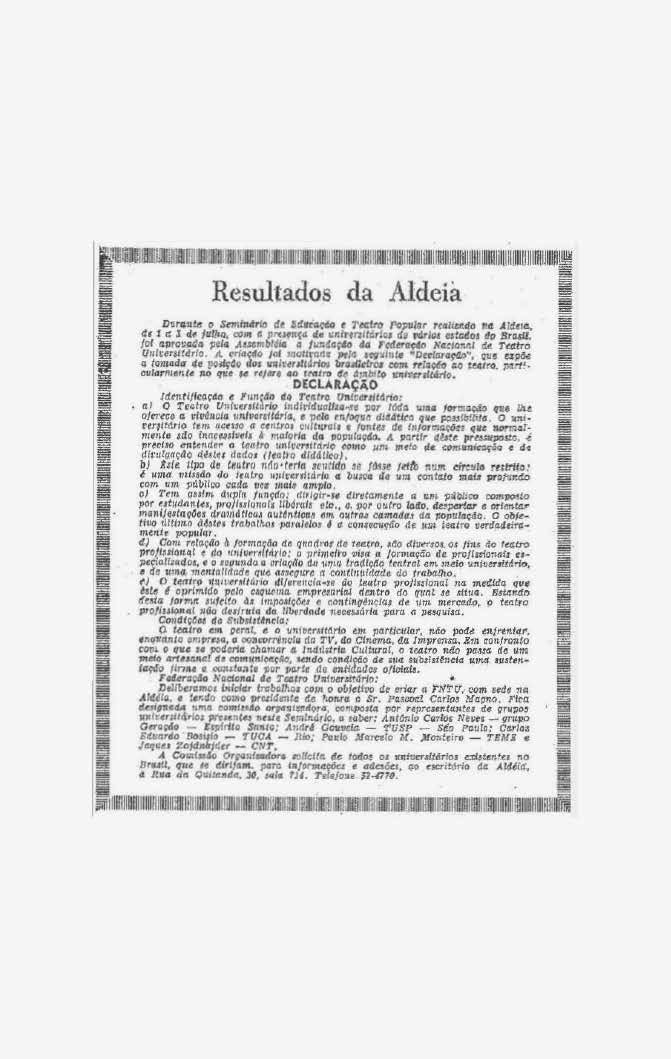
\includegraphics[width=\columnwidth]{./media/IMAGEM5.jpg}
\caption{{[}\textit{O Globo}, Rio de Janeiro, 7 jul. 1967, p. 5{]}}
\end{figure}

\section{Definição de uma estratégia estético-política}

É possível dizer que no intenso primeiro ano de existência do TUSP as
múltiplas atividades tinham ao mesmo tempo objetivos formativos e de
estabelecimento de uma orientação para a pesquisa artística. A
experiência do encontro em Arcozelo parece ter confirmado que o grupo
não teria uma só linha, e sim uma estratégia geral composta de muitas
etapas e ramificações.

Na \textit{Declaração} que expõe a “tomada de posição dos universitários
brasileiros com relação ao teatro”, podemos ler duas ideias muito
próximas das debatidas pelo TUSP, que provavelmente tiveram redação de
membros do grupo. A primeira é a consciência de que “o teatro
universitário diferencia-se do teatro profissional na medida que este é
oprimido pelo esquema empresarial dentro do qual se situa. Estando desta
forma sujeito às imposições e contingências de um mercado, o teatro
profissional não desfruta da liberdade necessária para a pesquisa.” A
pesquisa se apresenta assim, como um compromisso não-mercantil, do qual
o grupo não abriria mão. A segunda ideia é que deveria ser uma missão do
teatro universitário repartir socialmente a vivência de conhecimentos
que a universidade proporciona a seus integrantes:

\begin{quote}
O universitário tem acesso a centros culturais e fontes de informações
que normalmente são inacessíveis à maioria da população. A partir deste
pressuposto, é preciso entender o teatro universitário como um meio de
comunicação e de divulgação destes dados (teatro didático). Esse tipo de
teatro não teria sentido se fosse feito num círculo restrito. É uma
missão do teatro universitário a busca de um contato mais profundo com
um público cada vez mais amplo.
\end{quote}

Essa parte da Declaração enuncia em termos muito diretos o que seria o
primeiro espetáculo do TUSP. Teria que ter um enfoque \textit{didático} e
ao mesmo tempo ser \textit{popular}, não no sentido de uma comunicabilidade
fácil, ou da obrigação de transmitir padrões da arte elevada aos pobres,
mas sim o de estabelecer um diálogo de aprendizagem mútua, capaz de
“despertar” e até mesmo “orientar manifestações dramáticas autênticas em
outras camadas da população”, mas também de modificar os modos de
produção dos artistas-estudantes.

Tudo na história inicial do TUSP parece sugerir um duplo movimento, de
metamorfose e de autonomia. Os encontros com personalidades e grupos de
diferentes espectros políticos e artísticos foram úteis para a
compreensão das linhas de pesquisa artística em torno de um \textit{teatro
épico popular} aberto à cena documental. Os interesses do grupo pelo
teatro documentário, pelo Brasil modernista reinventado na arte
tropicalista, bem como a crítica à indústria cultural continuavam vivos
mesmo numa prática que teria Brecht como guia. Esses encontros foram
também úteis para o estabelecimento de estratégias de sobrevivência -
como as associações e o subsídio da CET aos grupos de teatro estudantil.
Ao mesmo tempo, não impediram que os estudantes mantivessem um
posicionamento político e artístico radical em relação a esses mesmos
interlocutores. O forte sentido de independência do TUSP tem relação
direta com a militância de alguns de seus membros, num momento de
disputa do movimento estudantil com a Ditadura, pela manutenção das
entidades representativas, quando da realização dos primeiros congressos
interrompidos pela polícia. Era necessário uma discussão verdadeira
sobre os rumos da esquerda brasileira.

O teatro universitário que daí surgiria procuraria táticas diferentes.
Ao mesmo tempo que reconheciam a força de seus mestres e modelos, era
necessário negá-los, diante das urgências atuais. Foi por isso que o
TUSP foi capaz de se referir ironicamente a seu professor Augusto Boal
como um “papa da festividade, renovador do teatro catártico”. E tratou
Zé Celso como alguém “devorado pela sociedade de consumo que tanto quis
devorar”.

Também nessa atitude negativa, o TUSP se inspirava neles, sendo incapaz
de se pôr numa posição subserviente. O sentimento do tempo, numa escala
mundial, era de um “estado de guerra”, como disse Régis Debray, o
estudante francês que abandonou seus estudos para se juntar à guerrilha
de Che Guevara na Bolívia, e escreveu em seus diários: “O estudante deve
se suicidar como categoria social para renascer como revolucionário.”

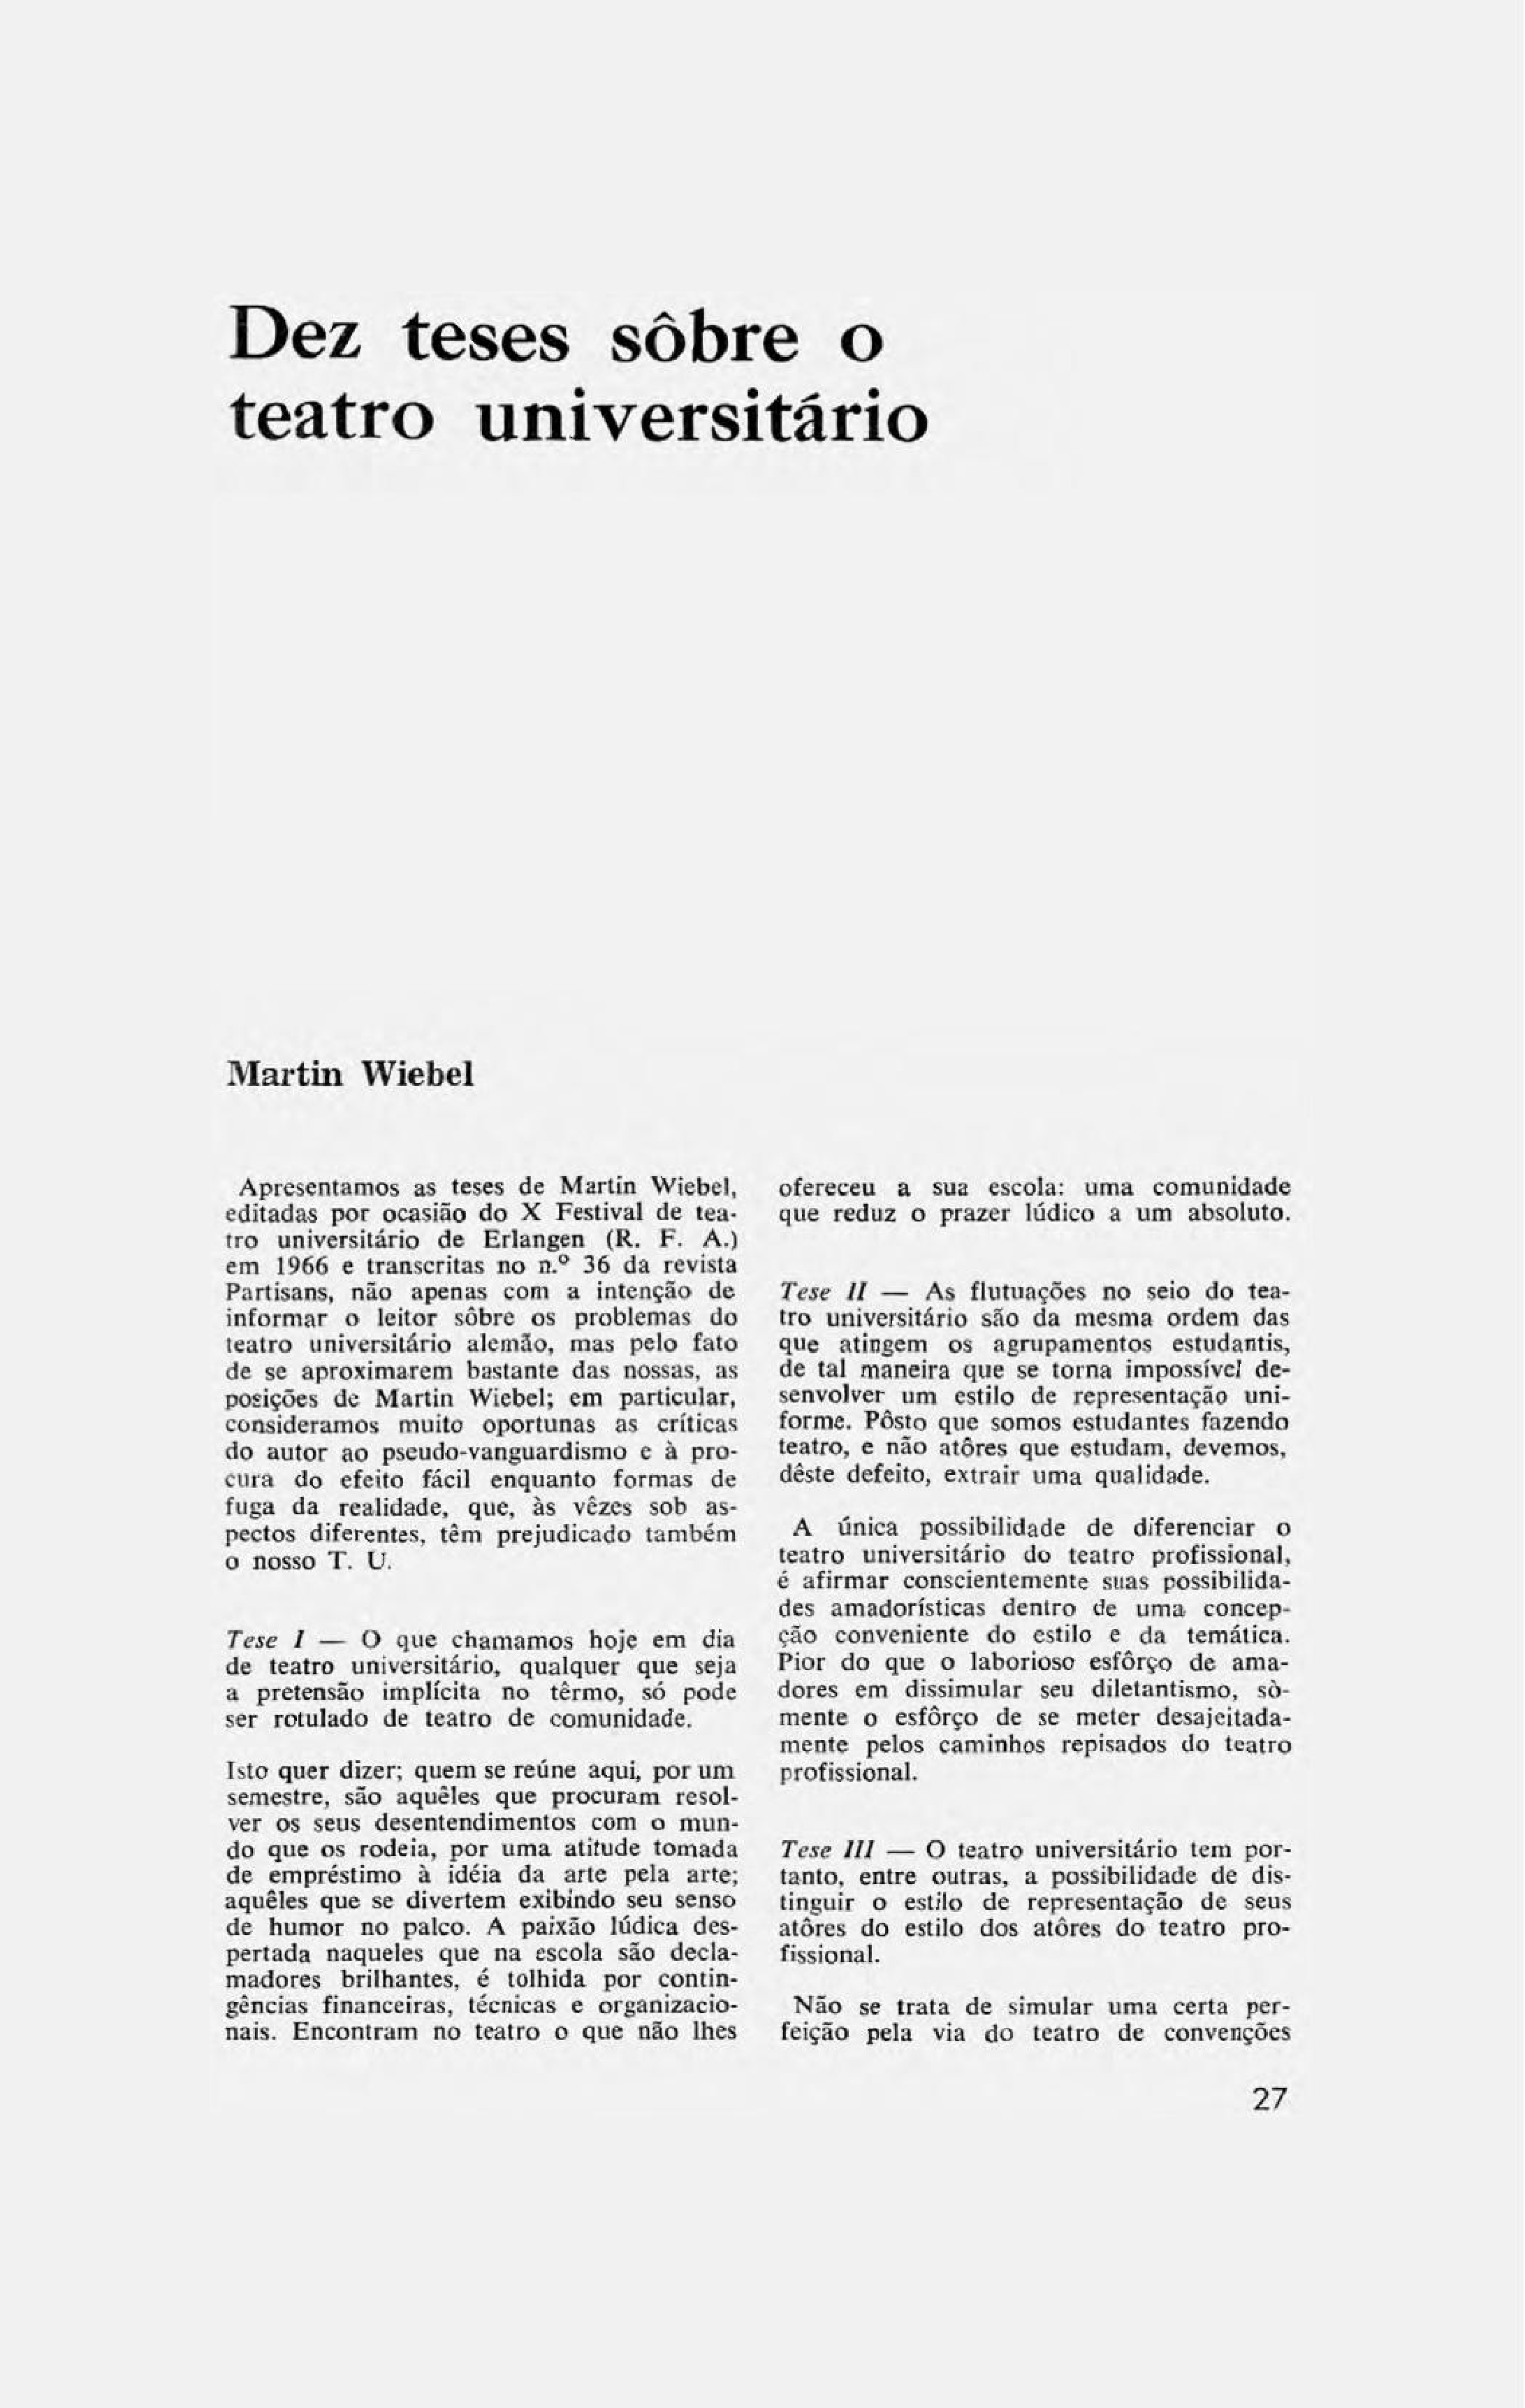
\includegraphics[width=\columnwidth]{media/DOC1.pdf}

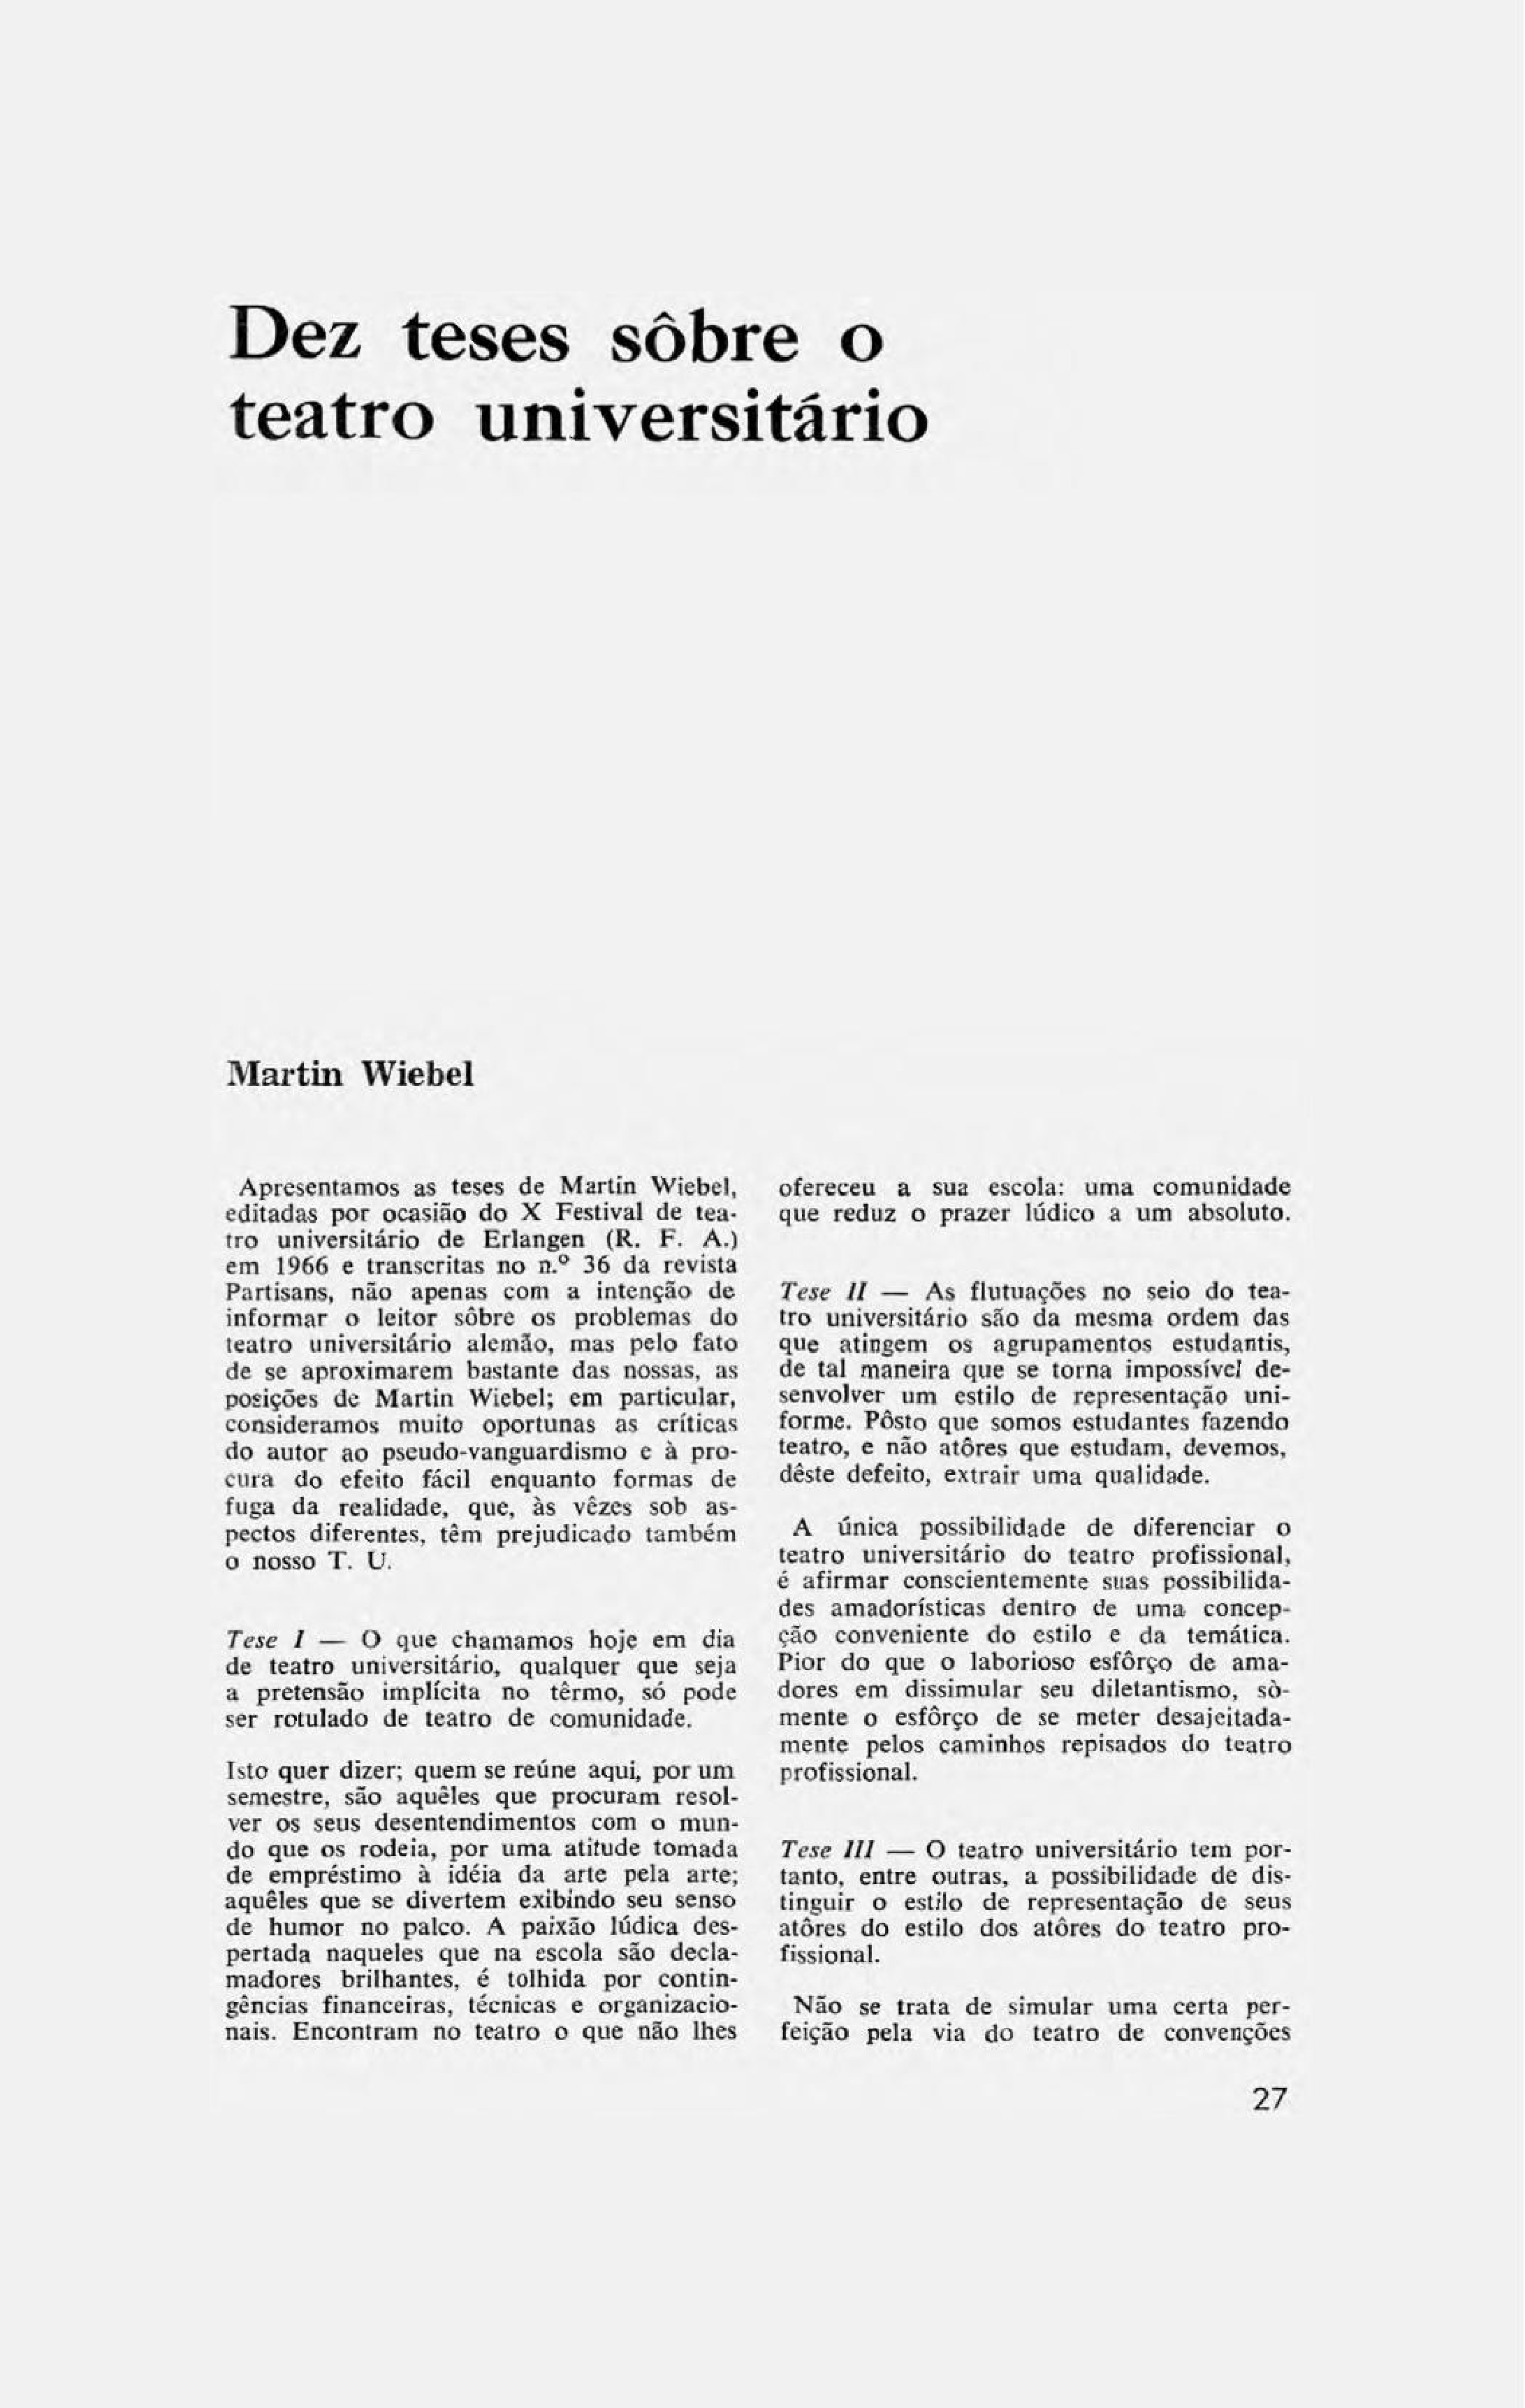
\includegraphics[width=\columnwidth]{media/DOC1.pdf}

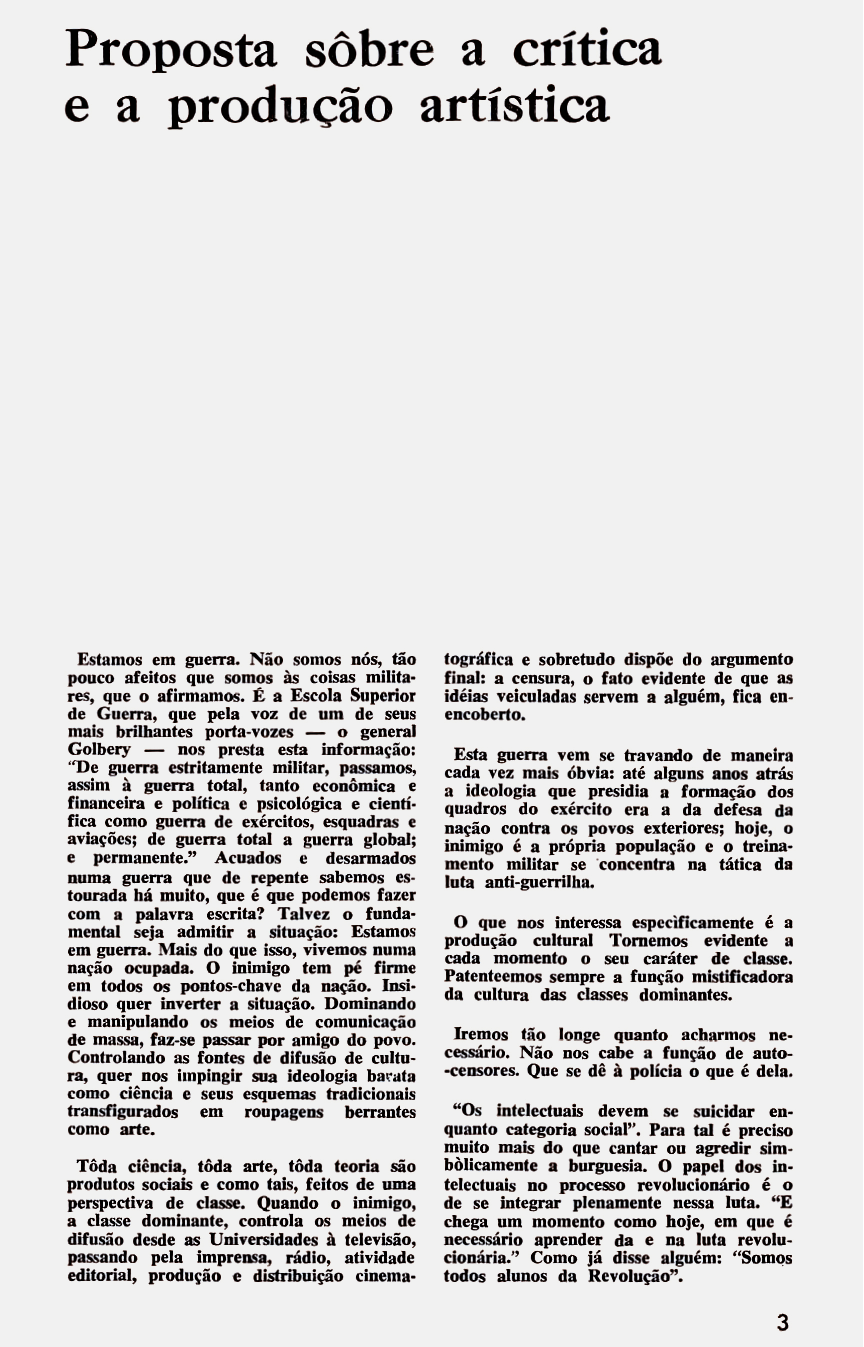
\includegraphics[width=\columnwidth]{media/DOC2.pdf}

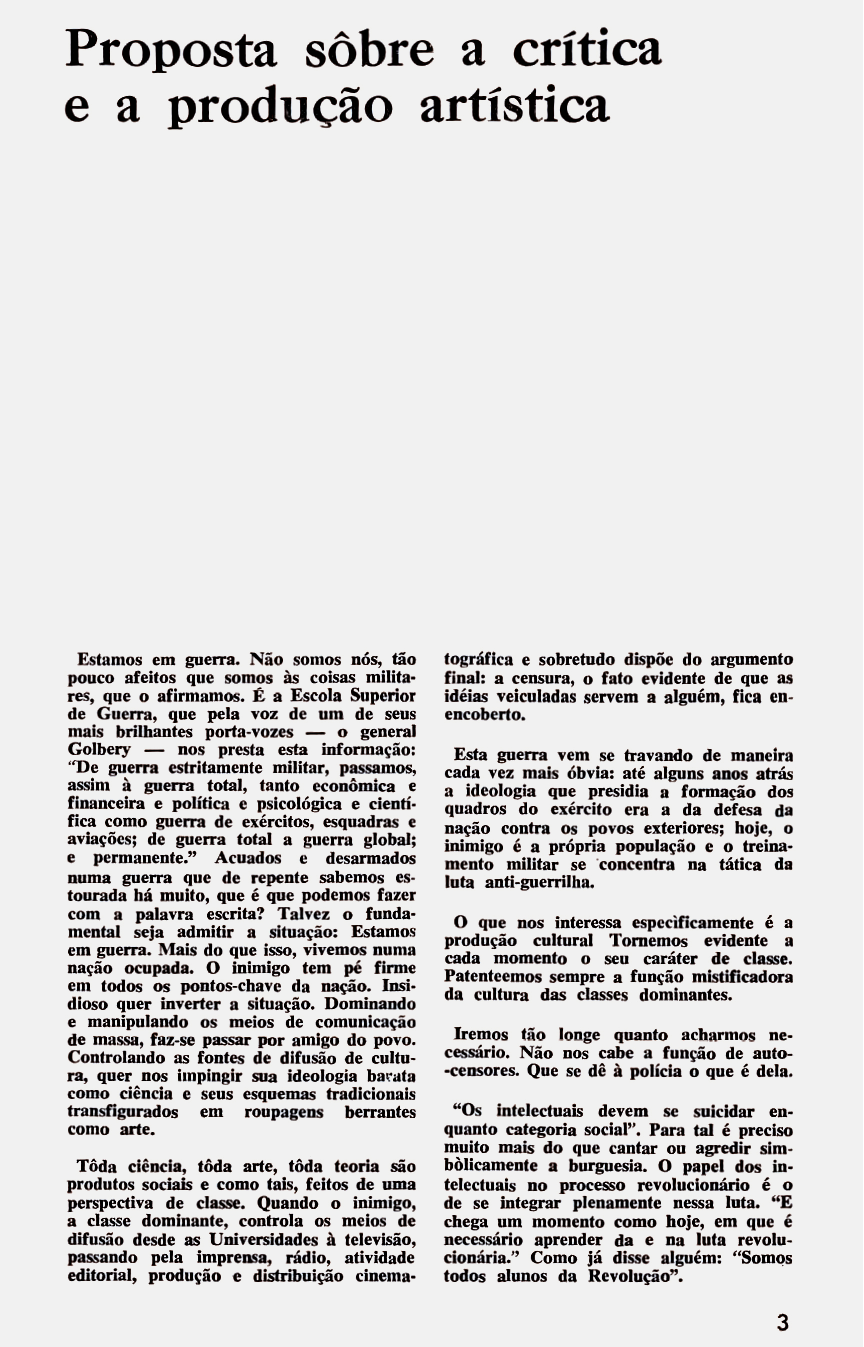
\includegraphics[width=\columnwidth]{media/DOC2.pdf}

\chapter{EXPERIMENTO DE TEATRO VOLANTE: \textit{A EXCEÇÃO E A REGRA}}

A escolha do material de trabalho é decisiva em qualquer processo
artístico. De sua definição dependem os movimentos futuros do projeto. E
se é verdade que um artista não escolhe seu assunto, mas é escolhido por
ele, é também verdade que o “chamado dos materiais” depende de uma
relação de procura anterior, que não se liga só a desejo ou intuição,
mas a uma consciência sobre o lugar de onde se parte. Para “observar é
preciso comparar”, dizia Brecht, “mas para comparar é preciso já ter
observado”.

Na procura dos caminhos de um teatro universitário de qualidade
artística, socialmente comprometido, e de interesse popular, a Comissão
de Dramaturgia decidiu encenar uma peça de \textit{teatro épico}. O texto
escolhido foi \textit{A Santa Joana dos Matadouros}, obra prima de Brecht
sobre o mercado de carnes de Chicago, que mostra uma grande crise
capitalista, com desemprego em massa e uma greve nos matadouros. Em meio
às violências do capital monopolista, ele apresenta o trágico
aprendizado da religiosa Joana, sobre a conciliação impossível na luta
de classes.

Concebida depois da \textit{quebra} da bolsa de 1929, \textit{Santa Joana} é
uma síntese dos estudos de marxismo e dialética que Brecht realizava
desde 1926. E contém um diálogo com o teatro político do tempo, na forma
dos corais irônicos e no interesse pela crítica à \textit{naturalização}
que oculta as causas dos problemas sociais: “a desgraça cai sobre nossas
cabeças de repente e sem explicação, como a chuva que nos molha sem que
ninguém seja culpado”, diz Joana aos trabalhadores. Sua forma literária
e teatral é complexa. A peça parodia versos clássicos da literatura
alemã e alterna diálogos e monólogos contraditórios com coreografias
quase operísticas dos desempregados, o que exige da equipe artística um
trabalho atento e de longo prazo.

A escolha de um texto, motivada pelo assunto, pela abordagem crítica e
pela beleza da forma também deve, entretanto, levar em conta a
capacidade do grupo em lidar com ele de maneira viva, atual e pessoal.
Ainda que na Comissão de Dramaturgia houvesse um tradutor da qualidade
de Roberto Schwarz - que mais tarde publicou sua versão brilhante da
obra de Brecht -, o TUSP, após a experiência de uma leitura pública da
peça, achou por bem adiar o projeto e começar com um texto mais simples:
\textit{A exceção e a regra}.

As razões para a mudança também se explicam por outro objetivo. O
primeiro espetáculo deveria servir para a formação artística da equipe e
ser uma encenação voltada a plateias populares, para apresentações em
salões de sindicatos, em associações de bairros, quadras de escolas e
faculdades, e não em palcos convencionais. O grupo queria mobilizar e
aprender com um público trabalhador e pobre, que raramente frequenta os
espaços culturais do centro da cidade.

\section{Modelos de teatralidade: a cena volante}

É possível dizer que a história da cena política do século XX se
confunde com a da cena móvel, que almeja sair do lugar de classe do
teatro convencional, ainda que no passado um movimento de trabalhadores
alemães tenha construído seu próprio teatro estável, a \textit{Volksbühne},
em Berlim, no padrão dos melhores teatros burgueses, numa época em que
milhares de operários associados foram capazes de sonhar com uma cultura
nova.

A tendência mais comum da cena engajada - quase uma regra estilística do
\textit{agitprop} - é a do espetáculo volante. A montagem é ensaiada como
um \textit{teatro de rua}. Ou ainda como um \textit{teatro na rua}, distinção
que se aplica quando a apresentação ao ar livre se vale de meios
técnicos como a amplificação sonora ou o palco montável, aparatos que
permitem a instalação de um “teatro” provisório num ambiente externo.

Foi como um \textit{teatro na rua}, por exemplo, que na década de 1930, o
poeta Garcia Lorca organizou sua lendária \textit{A Barraca}. O grupo de
artistas universitários levava, num pequeno caminhão, uma estrutura
cênica que permitia, em cada cidade, erguer um palco na praça, adaptável
às condições do espetáculo. O projeto cênico imitava as carroças cênicas
europeias do século XVI e XVII, sobre as quais se apresentavam artistas
ambulantes de grupos inspirados na então recente \textit{Commedia
dell´Arte}. Como acontece nos circos, a própria chegada desses coletivos
à nova localidade e a preparação da estrutura teatral eram
acontecimentos considerados teatrais pelas pessoas que acabavam por
ajudar o grupo, e depois assistiam ao espetáculo. A apresentação se
tornava, assim, uma parte intermediária de um “trabalho coletivo de arte
em processo” que termina após os debates e conversas que se seguem ao
espetáculo.

Lorca foi um dos principais artistas a aproximar a experimentação
modernista das formas e temas populares em seu país. Procurava
compreender as formas que persistem, oriundas da tradição pré-burguesa
do renascimento e do barroco, e ainda existem na cultura festiva ibérica
e dos territórios colonizados por Espanha e Portugal. \textit{A Barraca}
tornou-se legendária para artistas do mundo todo que, interessados numa
teatralidade antiburguesa, reconheciam a beleza integrativa dessas obras
do passado que não separavam do teatro a poesia, a dança e a música.

Seu trabalho inspirou no Brasil o Teatro do Estudante de Pernambuco,
fundado por Hermilo Borba Filho em 1946. E o posterior Teatro Popular do
Nordeste, que também realizaram a sua versão de \textit{A Barraca}, com
espetáculos móveis apresentados nos bairros e periferias de Recife. A
entrada de Ariano Suassuna no mundo da escrita dramatúrgica, com a peça
\textit{Uma mulher vestida de Sol}, é inspirada na cena e no projeto de
Lorca.

Pouco depois, em 1953, o Teatro do Estudante do Brasil produziu 15
caminhões adaptados como palcos que rodaram o país apresentando
espetáculos Essas influências ecoavam ainda no Movimento de Cultura
Popular de Pernambuco, projeto de arte que se conectava às Ligas
Camponesas.

No início dos anos 1960, o CPC da UNE realizou também diversas
intervenções de \textit{teatro na rua.} Eram cenas breves, escritas no
calor da hora, sobre um tema político importante do dia, baseadas em
figurinos e adereços alegóricos, como o do Tio Sam ou do
\textit{capitalista}. Esse grande projeto artístico-cultural reuniu
artistas profissionais e estudantes. Articulava teatro, cinema, música,
literatura e artes visuais. E também ele sonhou com sua carreta própria
que circularia pelo Brasil com o apoio do governo federal, para levar
\textit{autos} politizados a espectadores de todas as classes sociais.

A produtora e atriz Ruth Escobar, depois de 1964, conseguiu obter apoio
público para construir um grande palco volante sobre uma carreta, para
encenações ao ar livre, que chegaram a acontecer na praça da Sé, em
bairros periféricos e prisões. Seu repertório, evidentemente menos
politizado do que o do CPC, incluía obras de Suassuna como \textit{A Pena e
a Lei}. Inspirou-se no ideal de \textit{descentralização} tal como
formulado pelo Teatro Nacional Popular francês.

A cena itinerante pretendida pelo TUSP, em 1967, ainda continha algo
desse espírito modernista nacional-popular. Nas condições da crise da
esquerda comunista posterior ao golpe de 1964, sua perspectiva
socialista era internacionalizante. A forma pretendida deveria estar
mais próxima do \textit{teatro de rua}, em que o público poderia assistir à
montagem cenográfica, e eventualmente atuar como figurante na cena do
julgamento. E os temas não seriam locais, nem a forma teria elementos
reconhecíveis das tradições brasileiras. A peça seria mostrada como uma
parábola sobre a justiça numa sociedade dividida em classes.

\section{Estudo de formas cênico-dramatúrgicas: aprendizagem e agitprop}

O texto agora escolhido pelo TUSP foi uma das chamadas \textit{peças de
aprendizagem} ou \textit{peças didáticas} de Brecht. Em mais de uma
ocasião, o autor define essa modalidade inovadora de seu teatro nos
seguintes termos: é uma peça que “ensina porque é interpretada, não
porque é vista”. A peça se destina à aprendizagem de quem atua, não à
exibição ao espectador, ainda que o grupo possa aprender coisas novas
com as possíveis apresentações. São, portanto, textos-materiais,
imaginados como tentativas de superação ou mesmo de supressão do sistema
ator-espectador. E ao mesmo tempo estão abertas à invenção pessoal da
equipe que, com elas, praticava a \textit{dialética}. Apesar da
simplicidade estrutural, as \textit{peças de aprendizagem} pediam grande
experimentação na atuação e na música. Brecht considerava que apenas
algumas de suas peças podiam ser assim consideradas, aquelas que se
estruturam como estudos das contradições: \textit{A peça didática de Baden
Baden sobre o acordo, A exceção e a regra, Aquele que diz sim, aquele
que diz não, A decisão,} e \textit{Os Horácios e os Curiácios}.

É possível dizer que as \textit{peças de aprendizagem} se relacionam com o
momento de expansão dos grupos de \textit{agitprop} na Alemanha no fim da
década de 1920 como uma espécie de contraponto. Entre os muitos grupos
que orbitavam em torno do teatro político de Piscator, naquele tempo, o
mais importante era o \textit{Megafone Vermelho}, fundado em 1925, por
Maxim Vallentin com artistas da juventude comunista e inspirado no
lendário \textit{Blusa Azul} soviético. Com a turnê alemã do coletivo
soviético, ocorrida no final de 1927, num momento difícil da vida
econômica na República de Weimar, centenas de novos coletivos de
\textit{agitprop} foram formados na Alemanha, e é iniciada a construção de
uma federação europeia de teatro amador comunista.

Brecht, naquele mesmo ano, cria vínculos com essa cena politizada.
Colabora com Piscator e se aproxima da vanguarda musical que fazia
experimentos de arte operária no festivais de música que aconteciam em
Baden Baden, desde 1927. As \textit{peças de aprendizagem}, assim, foram
pensadas como experimentos em que os atores também aprendem ao cantar
aquelas composições notáveis de artistas como Kurt Weill e Hindemith.
Seu propósito fundamental - e assunto não-manifesto - é a prática
dialética. Os artistas aprendem enquanto assumem papeis diferentes nos
ensaios, quando vivem diferenças, e as compreendem de um ponto de vista
coletivo. A “verdade” narrativa não está encerrada numa única posição,
ela depende de um trânsito que não se completa dentro do palco. Baseadas
em parábolas, as \textit{peças de aprendizagem} mostram que os
comportamentos das personagens variam conforme aumenta a pressão de sua
função social. Existem muitos gestos num único gesto. A
\textit{aprendizagem} pela alternância e pela experimentação é sua dinâmica
e material pois tudo se dá sob o signo das contradições. É um teatro de
sentido negativo, radicalmente dialético, em que as oposições dualistas
são insuficientes. Corre o risco, inclusive, de parecer ambíguo demais
quando comparado à cena do \textit{agitprop} convencional, baseada na
denúncia, no reconhecimento ideológico, na definição mais nítida sobre
quem são os opressores e os oprimidos.

\section{Estudo da peça: A exceção e a regra}

A decisão do TUSP pela encenação de \textit{A exceção e a regra} como
alternativa a \textit{Santa Joana dos Matadouros}, trazia, assim, uma
dificuldade inesperada. A forma aparentemente simples do texto supõe uma
atividade cênica e social estabelecida, uma proximidade entre arte de
vanguarda e movimento operário e uma disposição a um teatro paradoxal
que não trabalha sobre identificações políticas diretas.

Uma das razões de sua escolha se ligava ao tema do enfrentamento das
ideologias. Assim como há em \textit{Santa Joana} uma crítica à
\textit{naturalização} das tragédias no mundo capitalista, \textit{A exceção e
a regra} desmonta imagens sociais hegemônicas através de gestos
concretos e simbólicos. Como em outras peças de Brecht, o texto reflete
discussões que estão em \textit{A Ideologia Alemã}, de Marx e Engels, sobre
as formas e os pensamentos dominantes como construções simbólicas que se
pretendem \textit{naturais}, como realizações histórico-culturais que se
afastaram do momento de verdade concreta do passado, e agora assumem a
aparência de uma universalidade abstrata.

O texto de Brecht abre com uma advertência coletiva, feita pelos
intérpretes do elenco. Utilizamos aqui a tradução de Roberto Schwarz
feita para o TUSP:

\begin{quote}
\textit{Observem muito atentamente}

\textit{Dessa gente o comportamento}

\textit{Vejam que é estranhável,}

\textit{embora não estranho}

\textit{Incompreensível, embora de regra}

\textit{Observem com desconfiança}

\textit{Mesmo o menor dos atos}

\textit{Aparentemente simples}

\textit{Verifiquem se ele é necessário}

\textit{Sobretudo se for costumeiro.}

\textit{Não achem por favor natural}

\textit{O que se faça diariamente}

\textit{Que nada seja assim natural}

\textit{Neste tempo de confusão.}
\end{quote}

O que se vê em seguida a esse pedido de \textit{estranhamento}, a essa
convocatória à \textit{desnaturalização}, é o começo da parábola de um
explorador e dois explorados em meio a uma expedição para o registro de
poços de petróleo no deserto. O grupo de viajantes é composto pelo
capitalista ocidental, pelo Guia contratado, e um trabalhador braçal que
suporta o peso da bagagem. Logo na primeira cena entendemos que existem
mediações naquela oposição dualista sugerida. Se a advertência já nos
pedia um olhar “estrangeirizador” sobre tudo, inclusive sobre a oposição
fácil entre os exploradores e os explorados, diante das personagens
percebemos que o movimento será diverso da tradição do \textit{agitprop}. A
exigência do Comerciante de mais violência física sobre o Carregador,
para que se apresse, não é uma ordem violenta de seu caráter, mas
motivada pela luta concorrencial. Existe uma segunda expedição que
pressiona o capitalista. De imediato, o opressor não é mostrado sob a
caricatura do “desumano” perverso: entramos na história através de sua
narrativa, feita no estilo do teatro japonês. O centro dramático da cena
é a hesitação do Guia sindicalizado em obedecer a ordem e punir
fisicamente o Carregador, essa figura pobre de um mundo colonizado, de
recente passado servil. Inesperadamente, é o Carregador quem resolve o
impasse ao pedir ao outro trabalhador que exerça de modo objetivo a
violência: “Bate-me, mas não demais, porque se é para chegar à Estação
Han, eu não posso empregar ainda a minha última força.”

A pancada do Guia hesitante no Carregador é o núcleo gestual da cena e
indica um movimento geral da peça, de sujeição consentida do trabalhador
precarizado, o que vai lhe custar a vida. Toda a primeira parte da peça
aprofunda a dialética inicial promovida pela disputa capitalista, à
custa da dor humana concreta. O avanço do sistema global \textit{high-tech}
repõe as práticas arcaicas do servilismo. Quando as dificuldades
crescem, o Guia sindicalizado não suporta mais seguir na tarefa de
mediar a exploração. A expedição entra, em seguida, numa zona mais
desértica. Não há ali polícia e leis, garantias do funcionamento social
da propriedade privada. No auge das tensões, a imposição da violência
passa a ser uma tarefa pessoal do patrão, que mais e mais teme o
descontentamento de seu Carregador. Este, mesmo com o braço quebrado,
segue no trabalho combinado. No pior momento do trajeto, quando
escasseia a água e a vida de ambos corre perigo, o Carregador oferece
seu cantil reserva ao patrão, num gesto de humanidade. Sem entender o
movimento inesperado, o Comerciante saca a arma e mata o outro.

A segunda parte da peça é o julgamento do crime. Conforme a tradição
recente do teatro político, Brecht mostra os esforços do Juiz para
liberar o Comerciante. Mas esta parcialidade de classe precisa ser
justificada segundo a lógica legal burguesa. O próprio assassino demora
a entender que a única saída será provar que agiu em legítima defesa.
Assim, de modo sinuoso, o Juiz desmonta a linha inicial do réu de se
mostrar como boa pessoa, faz com que venham à tona todos os horrores
promovidos por ele como indivíduo durante a expedição. E demonstra ser
inconcebível uma docilidade tamanha do Carregador, diante daqueles
excessos patronais. A expectativa classista na relação entre ambos
deveria ser óbvia. Entretanto, não foi de acordo com ela que o
Carregador agiu. Seu gesto solidário de dar a água ao seu algoz é
pessoal e inimaginável como comportamento de classe. O patrão só poderia
esperar uma contra-violência, supunha a pedra e não o cantil pois sabia
que estavam numa situação limite. Assim, o Juiz conclui que o
assassinato foi em legítima defesa diante da pedrada suposta, ainda que
não realizada. E o capitalista, na interpretação do Juiz, reagiu de modo
razoável ao supor o ataque nos termos da luta de classes, o que não
ocorreu do lado do trabalhador. Do ponto de vista capcioso do juiz
burguês, o comportamento do Carregador deve ser considerado um humanismo
fora de lugar e excepcional, enquanto o explorador esperava a reação
movida por um mundo desigual. Morto o Carregador e absolvido o
explorador, a família do primeiro fica sem sustento e não tem direito à
indenização.

Depois desse final desolador só resta ao público a reflexão crítica.
Quem tem direito à exceção e quem está obrigado à regra na sociedade de
classes? É uma das perguntas geradas por essa peça contraditória que
convoca o espectador à autocrítica social. Não há nela uma contraposição
dualista entre heroi e vítima, entre opressores e oprimidos. Não há
consciência de classe do lado dos trabalhadores. A maior vítima do
processo, o morto, não é sindicalizado, está distante do mundo dos
direitos básicos. E o Guia só se solidariza com o Carregador morto, não
com o vivo. O Carregador é o precário, o semi-escravizado da
modernidade. Precisa concluir a expedição para receber seu pagamento e
garantir o sustento de sua esposa e de seu filho pequeno. Não tem
condições históricas de rebelião.

A escolha de \textit{A exceção e a regra} como texto para a primeira
montagem do TUSP foi, portanto, das mais interessantes e produtivas. Mas
a rigor, sua simplicidade formal era aparente. Não correspondia a uma
peça política de mobilização, sendo antes uma espécie de falso
\textit{agitprop}. Ela exige um trabalho artístico criativo de atuação e
música, o que só confirmou a importância de mais intercâmbios de
aprendizagem com artistas profissionais.

Os estudantes perceberam que a dialética da peça, a ser realizada fora
do palco, exigia uma abordagem experimental, algo mais do que decorar o
texto e \textit{marcar} movimentos de cena. Porque eles não consideravam o
teatro uma confirmação de identidades, de exposição de vozes pessoais,
tentaram ir atrás do que não sabiam, à procura de aprendizagens que só
podem se dar na prática coletiva.

\section{Formação da equipe: artistas-pesquisadores}

O modo como o TUSP organizou as equipes de trabalho para o espetáculo
teatral reflete o modo como prepararam os estudos de formação do
coletivo artístico.

O elenco era de estudantes dispostos à aprendizagem teatral, de cursos
como arquitetura, medicina, engenharia e filosofia. No extremo oposto da
profissionalização, para a direção, foi convidado Paulo José, ator que
trabalhava com o Teatro de Arena e já havia dirigido uma leitura cênica
de \textit{O homem e o cavalo} com o grupo.

A escolha de Paulo José, artista brilhante, se deveu menos a sua
experiência como diretor, ainda pequena àquela altura, do que ao seu
talento de atuação e ao passado recente com o teatro universitário e
militante em Porto Alegre. Tinha um bom conhecimento da obra de Brecht,
formado nas discussões do Teatro de Equipe, do qual participaram
Fernando Peixoto, que se tornou um dos grandes divulgadores do teatro
épico no Brasil e Luiz Carlos Maciel, organizador da primeira coletânea
brasileira da teoria brechtiana, ambos influenciados por Ruggero
Jacobbi. Em 1961, Paulo José integrou-se ao Teatro de Arena de São
Paulo, onde atuou em montagens como \textit{Testamento de um cangaceiro},
texto de Chico de Assis, e \textit{A Mandrágora}, que fazia parte do
projeto de nacionalização dos clássicos empreendido pelo grupo antes de
1964. Suas atuações no cinema, a partir do sucesso de \textit{O Padre e a
Moça}, de Joaquim Pedro, aproximaram-no ainda mais dos artistas do CPC
que atuavam na cena politizada antes do Golpe, e ao mesmo tempo lhe
abriram caminhos para a televisão.

A aceitação do convite para colaborar com um grupo jovem no mesmo
período em que estreava no cinema \textit{Todas as mulheres do mundo},
filme de Domingos de Oliveira, e \textit{Bebel, Garota Propaganda}, de
Maurice Capovilla, é uma demonstração de sua abertura estética e
política, das conexões possíveis num momento em que a esperança por um
país melhor não era apenas uma expectativa imaginária. E indicava um
reconhecimento da força do movimento estudantil. Muitos anos depois,
quando Paulo José retornou à direção teatral após se aposentar da
televisão, colaborou com o grupo Galpão de Minas Gerais na montagem de
\textit{Um Homem é um Homem}.

Para o trabalho de cenografia e figurinos, o TUSP designou um núcleo da
Faculdade de Arquitetura. Mesmo antes da concepção cênica definida,
imaginaram fazer uso de uma estrutura metálica semelhante a um andaime,
que teria a função de servir como cenário, podendo ser montada e
desmontada rapidamente.

Entre os colaboradores indiretos da cenografia e da arte, havia artistas
como Claudio Tozzi. Em 1967, ano do assassinato de Che Guevara na
Bolívia, ele começou a expor sua bandeiras com as imagens do
guerrilheiro. As apresentações do TUSP levavam algumas dessas obras.
Apesar de não haver relação direta entre o tema da peça e os debates
sobre a luta armada sugeridos pelo artista plástico, esse imaginário
começa a rondar o ambiente de esquerda, e toma a frente do interesse do
grupo.

A própria Comissão de Dramaturgia participou ativamente do processo.
Jovens artistas e intelectuais assistiam aos ensaios do TUSP, que eram
abertos à comunidade de esquerda nos espaços universitários onde
ensaiava. Leituras cênicas abertas fizeram parte do processo. Eram
ocasiões de mostrar trechos e discutir com os presentes. Uma delas foi
feita acompanhada de poemas da peça \textit{Mãe Coragem e seus filhos}, em
tradução de Roberto Schwarz.

Na área musical, a Audimus, produtora de Damiano Cozzella e Rogério
Duprat, grandes maestros da Tropicália, foi convidada para fazer
releituras das composições originais de Paul Dessau, parceiro de Brecht,
que musicou o prólogo da encenação. Cozzella foi responsável pela trilha
sonora em encenações do Teatro de Arena no começo da década, como \textit{A
mandrágora} e \textit{O noviço}, ambas com direção de Boal e cenário de
Paulo José. Trabalhou com materiais de Brecht na montagem de \textit{A
ópera dos três vinténs} dirigida por José Renato em 1964 e, no mesmo
período da encenação do TUSP, colaborou com Duprat e Caetano Veloso na
trilha sonora de \textit{O rei da vela} do Teatro Oficina. Em \textit{A
exceção e a regra}, a ideia era que a música fosse executada ao vivo. E
isso, muitas vezes ocorreu. Sempre que possível havia o acompanhamento
sonoro do piano.

\section{Ensaios e laboratórios}

Não há documentos ou relatos precisos sobre os procedimentos de ensaio
utilizados no TUSP nessa primeira montagem. Paulo José, contudo, vinha
de uma experiência recente no Teatro de Arena em que o estudo do texto
era sempre acompanhado de um conjunto de improvisos conhecidos como
\textit{laboratórios}. Ainda que Boal reivindique para si essa
nomenclatura, associando-a à sua formação em Química, a expressão é
corrente desde o início do século XX para indicar situações de
experimentação teatral diversas de uma simples veiculação do texto pela
cena. A prática do \textit{laboratório} contém uma demanda de invenção
espetacular e cientificidade, aquilo que se poderia chamar de produção
de esboços para uma “escrita cênica”.

No Teatro de Arena, desde 1956, Boal aplicava princípios do realismo
stanislavskiano tal como conheceu em grupos influenciados pelo
\textit{Actors Studio}, em Nova Iorque. Mesmo nas montagens de um texto
pronto, os \textit{ensaios de mesa,} aqueles em que o texto é analisado do
ponto de vista das ações, eram completados por \textit{laboratórios} em que
os atores criavam situações emocionais variadas para suas personagens,
mergulhos vivenciais na ficção preparatórios ou complementares às cenas
escritas.

Num texto famoso em que resume aspectos técnicos da história do teatro
de Arena, Boal resume os procedimentos laboratoriais em operações que
parecem corresponder a uma estrutura de ensaio possível para um grupo
universitário.\footnote{Trata-se de \textit{200 exercícios para o ator e o
  não ator com vontade de dizer algo através do teatro}. (Rio de
  Janeiro: Civilização Brasileira, 1982, p. 36).}

Havia, de início, os \textit{exercícios de desmecanização}, em que o grupo
procura relaxar, soltar e liberar o corpo das tensões de todo tipo,
sociais e psíquicas, que produzem automatismos pouco perceptíveis pela
própria pessoa. O objetivo era “sair de si” para se livrar das próprias
“marcas registradas da atuação”. Dentro da série de
\textit{desmecanização}, Boal descreve os chamados \textit{exercícios de
emoção,} aqueles que acabaram por se tornar sinônimos de “fazer um
laboratório”. Em síntese, porque os procedimentos nessa linha são
muitos, tratava-se de intensificar a vivência emocional do mundo da
personagem com base em recursos variados que poderiam incluir as emoções
pessoais análogas (a famosa “memória emotiva”), mas com o intuito de
racionalizá-las à luz dos interesses da peça.

Boal desenvolveu, assim, uma “estrutura dialética da interpretação” em
que o grupo precisaria criar “rios em movimento dinâmico” e não “lagoas
emocionais” individuais. Era importante compreender que a personagem
surge dos olhos da outra personagem, da relação. Para tanto, era
necessário estudar, também isoladamente, as vontades de cada um e suas
contra-vontades. Cada conflito interno, quando posto numa situação
concreta, gera um movimento “dominante”, uma espécie de síntese
provisória que permite uma concretização da vontade como ideia, nos
termos do Teatro de Arena. Era preciso compreender esses elementos em
luta, suas interações contraditórias, dentro de si e na relação com o
outro, em meio às sucessivas variações (\textit{quantitativas}) do problema
da peça, o que geraria os saltos \textit{qualitativos}.

Sem a certeza exata do quanto esse procedimento foi aplicado em \textit{A
exceção e a regra}, é possível ao menos dizer que os jogos de
\textit{desmecanização} são úteis como ferramentas de liberação das
vergonhas e dos estereótipos que qualquer ator, mesmo os iniciantes,
assumem como máscaras sociais. O ambiente alegre e lúdico tantas vezes
produzido pelos exercícios têm efeitos coletivizadores. E podem
modificar a expectativa sobre a atuação, que costuma ser medida
convencionalmente pela força vocal da enunciação do texto, e pela
expressividade emotiva abstrata, critérios comuns na escala de valores
de um teatro corriqueiro.

\section{Análise social do texto}

Pelo conhecimento que temos do trabalho teatral posterior de Paulo José,
é possível dizer que nos ensaios do TUSP havia um atento esforço de
compreensão crítica do texto de Brecht, do ângulo de suas relações
sociais manifestas na forma.

Não estava em jogo somente a \textit{desmecanização} e preparação musical
do elenco com vistas a uma preparação técnica básica. A compreensão das
vontades, das contra-vontades e emoções numa peça de Brecht não podem se
dar num nível apenas psicológico, pois as figuras correspondem a tipos
sociais em lutas com a própria condição.

Numa peça de Brecht - para quem a menor unidade social é composta por
duas pessoas - é necessário entender qual o centro \textit{gestual} de cada
interação.

Um exemplo de que a dimensão sócio-política foi enfatizada por Paulo
José e pelos artistas do TUSP pode ser localizado na cópia de um texto
que pertenceu ao diretor, em que há poucas anotações, mas uma delas é
muito significativa.

Uma das cenas mais marcantes da peça de Brecht é aquela em que o
Comerciante impõe ao Carregador a travessia de um rio tumultuoso, que
está muito cheio. Mais do que um convencimento a uma tarefa de risco
estúpido, ao fim da qual o Carregador quebra o braço e quase morre,
existe na cena um jogo de linguagem em que a promessa irrealizável do
universalismo burguês é refeita de modo quase inconsciente pelo patrão e
aceita em termos linguísticos pelo trabalhador. Esse detalhe vivo, que
passa tantas vezes despercebido nas montagens, foi destacado no texto do
diretor por uma uma flecha que conduz à palavra “NÓS”, anotada como um
título no verso da cena para dar nome ao seu \textit{gestus} verbal. No
texto estão sublinhados ou grifados todos os momentos decisivos em que a
primeira pessoa do plural é utilizada ou como persuasão, pelo
Comerciante, ou como sinal de capitulação por parte do Carregador, que
só assume seu \textit{eu} quando percebe que será encoberto pelas águas. E
está também sublinhada a associação entre o suposto progresso trazido
pelo petróleo e a violência reprodutora do atraso:

O CARREGADOR: Viemos pelo caminho certo, senhor. O que se vê ali adiante
é o rio Mir. Normalmente, nesta altura do ano, ele não é difícil de
passar, mas no tempo da cheia ele puxa muito e é perigoso. Agora está
cheio.

O COMERCIANTE: \textbf{Nós} temos que atravessar.

O CARREGADOR: Muitas vezes espera-se oito dias, antes de atravessar com
segurança. Agora é perigoso.

O COMERCIANTE : Isso é o que nós vamos ver. \textbf{Nós} não podemos perder
um dia.

O CARREGADOR : Então \textbf{precisamos} achar um barco ou uma canoa.

O COMERCIANTE : Leva muito tempo.

O CARREGADOR : Mas eu nado muito mal.

O COMERCIANTE : A água não está tão alta.

O CARREGADOR: (Mete uma vara dentro da água) Mais alta do que eu.

O COMERCIANTE - Quando tu estiveres dentro da água, nada; porque daí não
tem outro jeito. Confesse, que nisso tu não tinhas pensado. Por que é
que \textbf{temos} que ir para Urga? Idiota, não és capaz de perceber que
\textbf{o petróleo vai ser um benefício para humanidade? Quando houver
petróleo, haverá estradas de ferro e bem-estar para todos.} Haverá pão e
roupas, e Deus sabe mais o que. \textbf{E isso, quem é que vai fazer? Nós}.
Depende tudo da nossa viagem.

\begin{figure}
\includegraphics[width=\columnwidth]{media/IMAGEM6_7.pdf}
\caption{FUNARTE/ Centro de Documentação e Pesquisa.}
\end{figure}

\includegraphics[width=\columnwidth]{media/IMAGEM6_7.pdf}

\section{Concepção em processo: a sala como tribuna}

Durante a criação de um espetáculo teatral, em determinado momento,
anterior ou posterior aos ensaios iniciais, criam-se condições para o
estabelecimento de um plano cênico. Brecht, por exemplo, rejeitava a
antecipação de qualquer concepção de encenação. Desprezava os diretores
que chegam no primeiro dia de ensaio com uma “visão” pronta ou ideia
estabelecida do espetáculo, com o desenho cenográfico ou o plano
espacial traçado, pois sabia da dimensão autoritária que há em impor aos
outros uma realização imaginária, sem verificar as muitas outras
soluções e caminhos possíveis propostos pela equipe. Para ele, ensaiar é
sempre \textit{pôr à prova}, desencadear crises a serem enfrentadas
alegremente. O talento do diretor está em “organizar a atitude de
surpresa” dos atores, em ganhar a confiança dos colaboradores de criação
cênica através da capacidade de indicar o que “não é uma solução”. Mas
mesmo uma concepção \textit{indutiva} da direção pede que algumas hipóteses
cênicas sejam imaginadas e experimentadas.

É difícil dizer de que modo a equipe lidou com a contradição de base de
seu projeto, entre o material dialético de uma \textit{peça de
aprendizagem} e a intenção afirmativa de uma montagem de \textit{agitprop.}

Pelos poucos documentos existentes, podemos supor que foi, entretanto,
na cena do tribunal que se procurou realizar uma síntese das duas
intenções, através da inclusão simbólica do público no debate jurídico.
Se em toda a primeira parte, o grupo parece ter feito uso de um teatro
épico de inspiração piscatoriana, com projeções, estrutura conográfica
aparente, títulos expostos, na segunda parte, a montagem se aproximou da
forma clássica da peça-tribunal, aquela em que o teatro jurídico deixa o
palco e acontece no conjunto da sala, convertida em participante de uma
espécie de drama analítico.

A peça-tribunal pode ser considerada um subgênero do teatro político.
São muitas as peças de Brecht que convergem para um julgamento ou que
têm cenas sobre juízes, sendo as mais célebres \textit{O círculo de giz
caucasiano} e \textit{A alma boa de Setsuan}. Sua forma aparece ou é
sugerida em outras peças de aprendizagem, como a \textit{A decisão} e
\textit{A peça didática de Baden Baden sobre o acordo}.\footnote{Um exemplo
  mais recente de uma peça de teatro político com estrutura de tribunal
  pode ser encontrado em \textit{A farsa da justiça burguesa}, de Sérgio de
  Carvalho. A fábula cria o julgamento de um sobrevivente do massacre de
  Eldorado dos Carajás, episódio em que a Polícia Militar do Estado do
  Pará matou 23 militantes do MST em marcha pela reforma agrária na
  região. A dramaturgia foi publicada no livro organizado pelo Coletivo
  Nacional de Cultura do MST - Brigada Nacional de Teatro Patativa do
  Assaré, \textit{Teatro e transformação social} (São Paulo: Centro de
  Formação e Pesquisa Contestado, 2007, vol. 2, p. 165-174).}

Em \textit{A exceção e a regra}, existe uma dialética temporal produzida
pelas duas partes. Quando chegamos ao momento do tribunal, o tempo da
travessia do deserto, antes observado como um presente dramático, é
rediscutido como passado. E a ação “presente” verdadeira se torna o
julgamento, aquele que interpreta em termos burgueses o que vimos do
ângulo do Carregador. A peça se desobriga, assim, do relato analítico do
passado, das explicações expositivas do caso, ou do recurso épico do
\textit{flashback}. O público pode se concentrar nos malabarismos
ideológicos de uma cena dramática que é “estranhada” pelo conhecimento
anterior da história. Se na primeira parte assistimos ao comportamento
do Carregador de modo distanciado, agora, diante de sua morte, sentimos
- com emoção - a dificuldade de resistir individualmente à lógica da
exploração. A cena-tribunal desse modo constituída, permite um
estranhamento do idealismo, algo que depende, entretanto, da atitude
coletiva produzida na sala.

É impossível dizer o quanto a montagem do TUSP conseguiu realizar suas
várias intenções artísticas e formativas. Mas a radicalidade do projeto
- em sua dimensão de aprendizagem - ainda hoje é modelar.

\section{Cenas de um experimento}

É impossível reconstituir a encenação desse espetáculo que se destinava
a uma primeira pedagogia - dos artistas universitários e de seu público.
O que sabemos é que o projeto se sustentou como esforço de oposição a
uma cena universitária que consideravam alienada do ponto de vista
produtivo; e pelo interesse em promover parcerias com entidades
representativas de trabalhadores, num momento em que elas estavam
enfraquecidas pela perseguição do regime. A história do espetáculo,
assim, vive na memória dos pequenos espaços onde foi representado, que
congregavam a classe trabalhadora. Há notícia de pelo menos uma sessão
no Sindicato dos Gráficos, duas no Sindicato dos Bancários e algumas
tantas no sindicato dos trabalhadores da Companhia de Cimento Portland,
em Perus, onde um grupo, que se autodenomina Queixadas, sustentou uma
mobilização contínua pelo reajuste salarial de 1962 a 1967. A duração do
movimento fez com que o sindicato fosse palco de diversas parcerias com
artistas, intelectuais e outros movimentos sociais. Na história de
teatro volante do TUSP foi talvez a experiência mais próxima daquela
vivida pelos grupos de \textit{agitprop} alemães, o lugar onde ocorreu a
colaboração mais integrada.

Foram realizadas apresentações ainda nos bairros da Lapa, Penha, Mooca,
Santo Amaro e Vila Mariana. Alguns espaços de mobilização estudantil
também receberam a montagem, como a Associação dos Estudantes de Santo
André, o grêmio da faculdade de Medicina da USP, parceiro do grupo, e
outras faculdades. Para chegar em diferentes territórios é fundamental a
parceria com pessoas que vivem e atuam na localidade. E a mobilização
artística do TUSP começou por aí, nos encontros preparatórios que
antecederam os espetáculos.

Do ponto de vista da forma cênica, as poucas imagens existentes de
\textit{A exceção e a regra}, não permitem dizer como se dava a relação com
o público. Mas ao certo era muito diversa daquela que ocorre num palco
italiano, com o apagamento das luzes, e ambientação cenográfica
ilusionista, que produz uma cena de quadro, disposta num espaço cúbico,
com a sugestão de uma relação contemplativa.

A estrutura cenográfica na montagem era, a um só tempo, palco e cenário.
Era montada à vista do público, que podia presenciar as dificuldades de
sua adaptação ao espaço. Os andaimes de construção civil delimitavam o
palco. Presa neles, ao fundo, uma lona branca fazia as vezes de
ciclorama, que servia para receber projeções e, ao mesmo tempo,
representava a infinitude do deserto onde se passa a ação.

Os andaimes são estruturas simples que dizem respeito ao mundo do
trabalho. Estavam ali deslocados de função: além de delimitar a cena e
sustentar a lona, permitiam que alguns refletores de luz fossem
pendurados. Estes eram usados na função tradicional de iluminar a ação,
mas também serviam a um jogo de luz em que se ampliava a silhueta dos
atores, segundo a técnica do teatro de sombras. As estruturas permitiam
elevações dos atores nas ocasiões de má visibilidade, pelo excesso de
público ou pela ausência de arquibancadas.

É também de se imaginar que houvesse um “aquecimento” do elenco
realizado à frente dos espectadores. O que se sabe de concreto é que o
prólogo do espetáculo era realizado com uma canção cantada em coro pelo
elenco. E todos os números cantados eram acompanhados de projeções das
letras, o que anunciava seu caráter narrativo, e permitia que o público
cantasse junto.

Quando tinha início a história do Comerciante, do Guia e do Carregador,
eram suas presenças que determinavam os movimentos da luz e da projeção,
e não o contrário. Apesar da aparência de um canteiro de obras, havia um
cuidado estético nesta cena de tantos arquitetos. Esse modo de projetar
imagens sobre o cenário e os atores ecoava as descrições das encenações
épicas do diretor alemão Erwin Piscator, cujas estruturas cênicas muitas
vezes também se constituíam de andaimes e lonas. Brecht observa que a
genialidade de Piscator na adoção desse elemento se devia ao fato dele
rejeitar o uso convencional de apenas trocar o cenário ilusionista
construído pela projeção. Piscator empregava a projeção como se fosse um
ator a mais, uma imagem transformável pelos agentes humanos da cena.

Paulo José optou por uma concentração artística nesses três elementos
básicos: a atuação, a música, e as projeções e sombras sobre a lona e as
estruturas, na tentativa de pôr em cena a aprendizagem ainda inicial do
grupo. A beleza da montagem e suas eventuais dificuldades na relação com
os espectadores que conheciam pela primeira vez tem a ver com essa
intenção que priorizou o processo sobre o resultado. A politização
produzida pelo primeiro espetáculo do TUSP era gerada pelo próprio
trabalho teatral, no intuito de um sentido novo ao amadorismo e ao
teatro universitário.

Se \textit{A exceção e a regra} fracassou como teatro de mobilização
política, como consideram hoje alguns de seus artistas, talvez não tenha
fracassado como \textit{teatro de aprendizagem}.


\begin{figure}
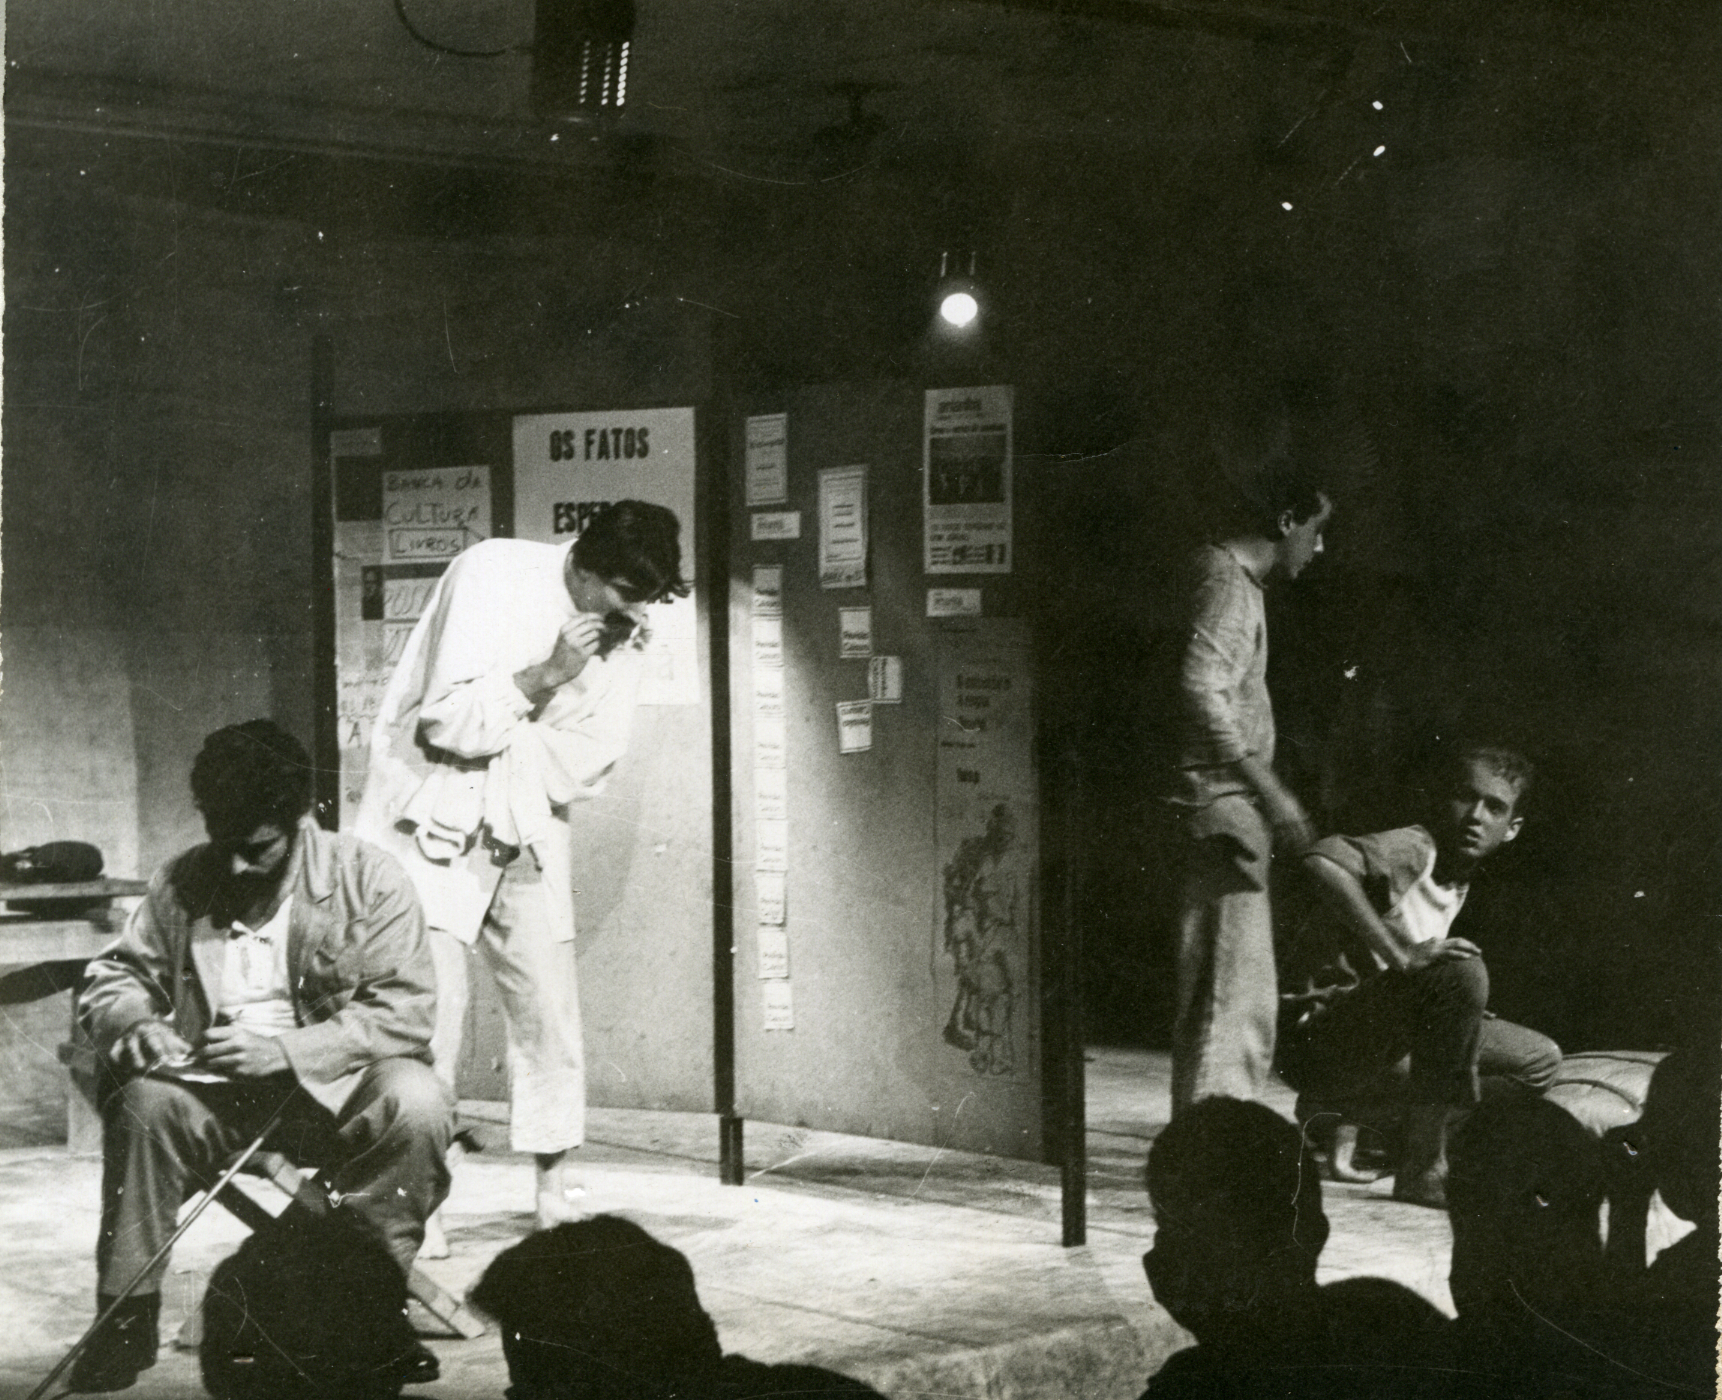
\includegraphics[width=\columnwidth]{./media/IMAGEM8.png}
\caption{Atores antes da apresentação no Sindicato dos Bancários. Sérgio Mindlin
como o Comerciante, André Gouveia como o Guia, ator não identificado e
Rudolf Mayer-Singule como Juiz. Autor desconhecido. Acervo dos Diários
Associados. Arquivo Público do Estado de São Paulo.}
\end{figure}

\begin{figure}
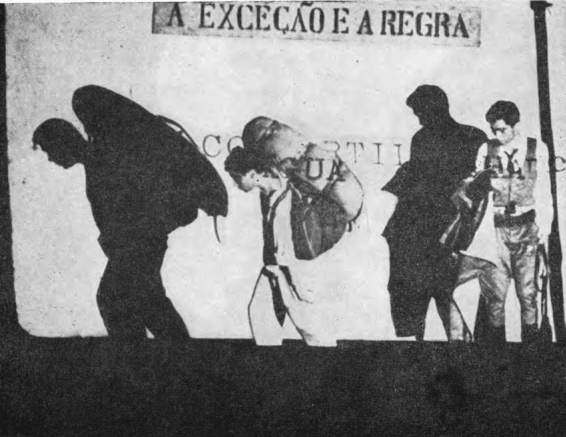
\includegraphics[width=\columnwidth]{media/IMAGEM9.png}
\caption{Projeção e sombras em \textit{A exceção e a regra}. Ator não identificado
como o Carregador e André Gouveia como o Guia. Autor desconhecido.
\textit{aParte}.}
\end{figure}

\chapter{TEATRO DE GUERRILHA COMO IDEIA EM DISPUTA}

O conceito \textit{teatro de guerrilha} - que pode ser associado de modo
apenas indireto ao TUSP - surge da cena radical e independente que
ganhou espaço nos Estados Unidos na segunda metade do século XX, num
momento de crescimento da cultura política, no auge da Guerra Fria,
quando revoluções e guerras de libertação nacional ocorriam no sul
global.

A agitação e propaganda da década de 1960 ainda se inspirava nas
práticas de \textit{agitprop} desenvolvidas nos anos 1920 e 1930, mas
procurava incorporar em seus procedimentos as sugestões extraídas dos
escritos dos revolucionários admirados em sua época, como Che Guevara e
Mao Tse-Tung, líderes que imprimiram às táticas de guerrilha uma
dimensão de politização e convocatória popular.

Os grupos artísticos que num sentido rigoroso praticaram um \textit{teatro
de guerrilha} foram os que estiveram nas frentes de batalha na China, no
Vietnã e na Nicarágua. A divulgação mundial de suas práticas corajosas
foi imediata. O TUSP, por exemplo, publicou na revista \textit{aParte} o
roteiro de \textit{Phin Phong Su}, um filme produzido pela Frente de
Libertação Nacional do Vietnã. O texto de apresentação informa que
“antes de mais nada, um ‘cineasta' vietcong é um guerrilheiro totalmente
integrado na luta contra a agressão americana no Vietnã do Sul.” Além de
suas funções de combate, ele deve produzir vídeos de divulgação do
avanço da guerrilha, ou informativos que ensinam como se maneja uma nova
arma que foi expropriada do exército americano.

O mesmo se dava com os artistas teatrais que se integraram às guerrilhas
nas zonas de combate. Há uma história significativa sobre o período em
que os norte-americanos cercaram as aldeias no Vietnã. Um grupo de
teatro atravessava todas as noites o cerco para apresentar uma peça
repleta de símbolos e sugestões que ensinavam aos agricultores como a
luta deveria ser travada. Certa noite, os agricultores compreenderam a
mensagem codificada e, na manhã seguinte, atacaram e destruíram os
pontos estratégicos da própria aldeia, para dificultar o domínio dos
invasores.\footnote{A história, narrada por Armand Gatti em uma
  entrevista ao periódico alemão \textit{Die Zeit} em julho de 1969, é
  recuperada por Martin Maria Kohtes, que realizou o estudo mais
  sistemático sobre o conceito \textit{teatro de guerrilha} em
  \textit{Guerrilla Theater: theorie und praxis des politischen
  Strassentheaters in den USA (1965-1970)}. (Tübingen: Gunter Narr,
  1990, p. 15).}

\section{Conceito estadunidense de Teatro de guerrilha}

O \textit{teatro de guerrilha} tal como elaborado nos Estados Unidos não se
deu no âmbito do \textit{agitprop} que colabora com uma guerrilha armada
real. A expressão surge antes como uma metáfora, uma orientação poética
para que o teatro de esquerda das grandes cidades do Ocidente se pense
numa relação de analogia com a luta de libertação vietnamita, e também
faça uso da reflexão de revolucionários como Che Guevara, conforme as
proposições do ensaio mais famoso sobre o tema, escrito em 1965 por R.
G. Davis, fundador da \textit{San Francisco Mime Troupe}, e publicado na
revista \textit{Tulane Drama Review}, no verão de 1966.\footnote{O texto de
  Davis foi republicado como apêndice em \textit{The San Francisco Mime
  Troupe: the first ten years}. (Palo Alto: Ramparts Press, 1975, p.
  i-iv).}

Fundada sete anos antes, a \textit{San Francisco Mime Troupe} fazia teatro
em parques públicos ao menos desde 1962. Antes de assumir-se como um
grupo de teatro de guerrilha, vinha influenciando a retomada do teatro
na rua em seu país, sendo um dos mais conhecidos grupos de teatro
politizado do tempo, ao lado do \textit{Living Theatre} (de Judith Malina e
Julian Beck), do \textit{Bread and Puppet} (de Peter Schumann) e do
\textit{Black Revolutionary Theatre} (de Amiri Baraka).\footnote{Entre os
  muitos grupos politizados do período, podemos citar ainda o Open
  Theatre (sob a direção de Joe Chaikin) e o Performance Group (liderado
  por Richard Schechner).} Teve ainda participação direta na criação de
outro coletivo fundamental na crítica anticapitalista, o \textit{El Teatro
Campesino} (fundado por Luis Valdez).

Nos textos e manifestos dessa geração, encontramos imagens que mostram a
radicalidade desses artistas no que se refere à não-conciliação com a
cultura dominante. Amiri Baraka, que então assinava LeRoi Jones, observa
sobre os caminhos do teatro negro fundado por ele:

\begin{quote}
o Teatro Revolucionário, mesmo que seja ocidental, deve ser
antiocidental. Deve mostrar as horríveis atrações futuras de \textit{A
queda do Ocidente}. Assim como Artaud projetou \textit{A conquista do
México}, devemos projetar \textit{A conquista dos olhos brancos} e mostrar
os missionários e os liberais rebeldes morrendo sob explosões de
concreto. Como efeito sonoro, gritos selvagens de alegria de todos os
povos do mundo. O Teatro Revolucionário deve pegar os sonhos e torná-los
realidade.\footnote{Seu manifesto \textit{The Revolutionary Theatre} foi
  publicado em uma das revistas mais radicais da imprensa negra,
  \textit{Liberator} (vol. V, n. 7, july 1965).}
\end{quote}

Se é verdade que o \textit{teatro de guerrilha} tinha menos ímpeto
poético-revolucionário do que o sugerido por Baraka, ele procurava, por
outro lado, constituir uma técnica artístico-política transmissível, de
caráter prático e sentido anti-imperialista.

O ponto de partida do artigo de Davis é uma frase de Che Guevara em
\textit{Guerra de Guerrilhas}, sobre a revolução em Cuba. Contra a
alienação de uma sociedade como a dos Estados Unidos em relação à Guerra
do Vietnã, o teatro deveria assumir um programa triplo: “ensinar,
direcionar para a transformação, e ser um exemplo de transformação”.
Deveria comportar-se, portanto, como um foco de guerrilha na disputa
ideológica, e procurar lugares sociais onde existam desejos reprimidos
de mudanças. Os atores na cidade comportam-se como os guerrilheiros que,
através de seu exemplo, motivam a aldeia a participar da guerra.

A argumentação de Davis espelha o pensamento de Guevara. Também o teatro
deve fazer o reconhecimento prévio do terreno onde será realizada sua
apresentação; manter o princípio de nunca enfrentar o inimigo
reacionário de frente; carregar pouca bagagem, de modo a facilitar a
possível fuga. Deve adotar, enfim, o procedimento do \textit{ataca-e-foge},
também conhecido como o “morde e foge”, valorizado por Che Guevara:

\begin{quote}
‘Morde e foge' diziam algumas pessoas, de modo depreciativo, sobre a
atuação da guerrilha. Mas esta observação é exata: morde e foge; espera,
espreita, volta a morder e fugir. E, assim, sucessivamente, sem dar
descanso ao inimigo.\footnote{Che Guevara precisa a tática em seu
  célebre \textit{Guerrilha} publicado pela primeira vez no Brasil pela
  Editora Base, da ALN (Ação Libertadora Nacional) ({[}São Paulo{]}:
  Editora Base, 1968, p. 51).}
\end{quote}

Davis sublinha a importância de que o espetáculo teatral ajude a
construir uma relação comunitária com o público, assim como Guevara
ressalta a importância do apoio popular ao lutador revolucionário. Não
virá dos dos artistas a força para enfrentar o risco político da
criminalização de sua arte, como aconteceu com a \textit{San Francisco Mime
Troupe} em 1965, quando o grupo teve cassada a autorização para
apresentações públicas em parques da cidade e decidiu realizar, mesmo
assim, o espetáculo ao seu público, que os aguardava. Davis deu início à
encenação e ela durou os momentos necessários para convocar a plateia a
acompanhá-los durante a prisão. Foram os espectadores que evitaram a
violência policial e levantaram fundos para o pagamento da fiança.

Em um texto de 1968, \textit{Cultural Revolution USA}, Davis afirma que
Fidel Castro pretendia a conquista do poder e a posterior eliminação do
exército, enquanto “nós, como guerrilheiros culturais, pretendemos: 1) a
conquista do poder; 2) a eliminação da mentalidade burguesa”.\footnote{O
  texto consta no já citado \textit{The San Francisco Mime Troupe: the
  first ten years}. (Idem, p. vii).}

Richard Schechner, artista que também escreveu sobre o \textit{teatro de
guerrilha} com base no trabalho de seu \textit{Performance Group}, é quem
afirma que esse projeto, nos termos de Davis, é uma \textit{ação
simbólica}. Para ele, o nome viria da adaptação das formas da luta
revolucionária, do aprendizado da luta dos mais fracos contra os grandes
inimigos, o que gera algumas tendências: a simplicidade das táticas, a
mobilidade constante possível a grupos pequenos, a atuação nos pontos de
vulnerabilidade, e o elemento surpresa.

Davis, por sua vez, deu forma a um debate que chegará aos grupos de
teatro politizado fora dos Estados Unidos, e que levou à uma indagação
recorrente: quais as formas eficazes de um teatro engajado na
atualidade, diante do crescimento das indústrias culturais e das
mudanças no imaginário popular?

Sua posição quanto a isso, é a de que o teatro politizado deve
apresentar espetáculos melhores do que aqueles vistos no teatro
comercial, para compensar a falta de publicidade e de equipamentos. Os
artistas precisam sentir-se obrigados a atrair o público pela atuação e
dramaturgia, para além de qualquer expectativa de simpatia ou de
concordância ideológica. Segundo ele, se o conteúdo da peça for muito
fechado, torna-se datado. Se for muito alegórico ou acadêmico, o público
irá rejeitá-lo.

Num tempo em que a cena de vanguarda oscilava entre as posições poéticas
de Brecht e Artaud, que tinham em comum o ideal de uma superação radical
do teatro burguês, um grupo politizado seria inevitavelmente levado
(como disse Amiri Baraka) a fazer uso de suas ideias, mesmo que para
negá-las. Para Davis, Brecht era o teatrólogo mais útil deles quando se
pretendia superar o drama psicológico estadunidense porque evitava o
salto artaudiano de uma recusa fácil da racionalidade burguesa, o que
muitas vezes conduz à “selva” da “improvisação instantânea, criação
instantânea e café instantâneo: todos meio aguados”. Davis afirma que
qualquer coisa capaz de abalar a cultura do \textit{American way of life}
será bem-vinda, mesmo que europeizante. Por outro lado, no que se refere
a uma comunicação artística popular, o teatro deveria procurar
referências nas formas locais: “talvez o beisebol seja a melhor
inspiração”, retomando uma antiga associação entre teatro e esportes.

Na parte final de seu texto, ele propõe um conjunto de observações
práticas: indica o melhor formato e peso de um palco volante e dos
adereços; sugere o uso politizado de formas espetaculares como
\textit{Commedia dell'Arte}, o \textit{vaudeville}, os “menestréis”
estadunidenses; e recomenda o uso de uma banda de \textit{rock}, entre
outras sugestões de como atualizar a peça, de como organizar ensaios e
realizar a produção executiva.

O conjunto de reflexões sobre o \textit{teatro de guerrilha} pode ser
considerado, assim, uma parte de um movimento histórico em que as
universidades se tornaram lugares de disputa política, quando a
politização de esquerda vivia a crise do padrão soviético dos partidos
comunistas, e surgiram novas pautas de reivindicação, num processo
global que tem seu símbolo maior nas ocupações de Paris em maio de 1968.

Na Califórnia, onde a \textit{San Francisco Mime Troupe} atuou, os anos de
1964 e 1965, foram de ebulição política, em torno do Free Speech
Movement (FSM), de Berkeley, pela liberdade de expressão. Os estudantes,
influenciados pelo Movimento pelos Direitos Civis contra o racismo e a
segregação racial e pelas posições da Nova Esquerda, amparada pelos
debates da Escola de Frankfurt, realizaram atos de desobediência civil
dentro do \textit{campus} que foram violentamente reprimidos. Alguns deles
repercutem no estilo de mobilização estudantil até hoje. Começava ali um
momento da política em que pautas até então pouco consideradas pela luta
revolucionária clássica - relativas a raça, gênero, sexualidade,
política de drogas, entre outras - assumiram o centro das mobilizações.

A Mime Troupe colaborou com esse movimento. Quando saíam em turnê, sua
sede era disponibilizada para a New School, um dos primeiros projetos de
“universidade livre” a surgir na esteira do Free Speech Movement.

A luta de classes, entretanto, seguirá sempre em pauta enquanto existir
o capitalismo. Em 1965, ao sul da Califórnia, eclodiram greves de
trabalhadores rurais. Numa cidade marcada pela imigração latina, Delano,
houve um grande enfrentamento. Luis Valdez era filho de imigrantes
mexicanos da região. Acabara de ingressar na \textit{San Francisco Mime
Troupe} e aplicou as técnicas aprendidas no grupo teatral em ações de
\textit{agitprop} para o movimento grevista. Ofereceu aos líderes sindicais
a possibilidade de organizar um grupo artístico, o que foi o começo de
\textit{El Teatro Campesino}, primeiro projeto de teatro \textit{chicano} dos
Estados Unidos, majoritariamente composto por trabalhadores rurais. As
encenações eram bilíngues, repletas de canções em castelhano. O Teatro
Campesino ficou conhecido por seus divertidos \textit{Actos}, com divisão
de personagens indicada por placas. Havia figuras frequentes em suas
apresentações: o Esquirol {[}fura-greve{]}; o Patroncito {[}patrão{]}; o
Contratista {[}capataz{]}; e o Huelguista {[}grevista{]}. O grupo
constituiu, assim, uma obra teatral notável, de atuação integrada ao
cotidiano camponês, com intervenções que informaram os trabalhadores
sobre os movimentos grevistas e o andamento das negociações do
sindicato.

Em pouco tempo, o \textit{teatro de guerrilha} expandiu-se em todo os
Estados Unidos. Em 1966, alguns dissidentes da Mime Troupe fundaram o
coletivo anarquista \textit{Digger}s, que propunha uma direta \textit{atuação
na vida} (“life-acting”). Não queriam representar, mas “atuar”.
Ligavam-se ao movimento \textit{hippie} e criaram atividades públicas: uma
imprensa alternativa, que divulgava notícias pela cidade; um transporte
que levava gratuitamente as pessoas a Berkeley; uma rede de alimentação
gratuita; e espaços de comércio, de serviços médicos, e jurídicos,
oferecidos à população. Além disso, organizaram ações culturais, como
shows de grandes bandas.\footnote{De acordo com Michael William Doyle em
  “Staging the Revolution: Guerrilla Theater as a Countercultural
  Practice, 1965-1968”, a viabilidade desse conjunto de ações se liga a
  uma conjuntura muito específica: o trabalho de uma juventude branca de
  classe média que muitas vezes podia contar com o suporte familiar,
  doações desses artistas musicais e até de traficantes de psicodélicos
  e de proprietários de comércio, que lucravam com a curiosidade
  despertada pela Cidade Livre instituída no bairro de Haight-Ashbury,
  em San Francisco, o grande excedente de bens com o \textit{boom}
  econômico da segunda metade da década de 1960, o dinheiro injetado na
  baía, ponto de saída para o Vietnã, o custo de vida relativamente
  baixo em San Francisco na época e até o clima ameno. O texto foi
  publicado no livro editado por Doyle e Peter Braunstein, \textit{Imagine
  Nation: The American Counterculture of the 1960s and '70s} (New York:
  Routledge, 2002, p. 71-97).}

Pode-se citar em linha semelhante o coletivo \textit{Yippies}, cujo nome
vem do \textit{Youth International Party} (Partido Internacional da
Juventude). Surgiram em 1968, em Nova Iorque, e realizavam
\textit{happenings} escandalosos, para os quais convocavam a mídia
burguesa, no intuito de divulgarem imagens anticapitalistas. Sua
primeira e mais famosa ação foi uma visita à bolsa de valores de Nova
Iorque. Da galeria de visitantes eles jogaram punhados de notas de
dólares sobre os funcionários do pregão, num gesto registrado por
repórteres.\footnote{Suas ações adotaram esse formato de
  \textit{happenings}, sempre contando com a mídia como palco. Seu mais
  ambicioso projeto, a realização do Festival da Vida durante a
  Convenção dos Democratas em Chicago, um grande projeto de divulgação e
  politização da contracultura, foi frustrado por uma violenta
  intervenção policial.}

O \textit{American Playground}, de Marc Estrin, era outro desses grupos que
assumiam o nome \textit{teatro de guerrilha} para suas intervenções
performáticas. Os atores do grupo se misturavam à população em metrôs e
praças e simulavam um acontecimento problemático, de modo a estimular
debates no público, em padrões muitíssimos semelhantes aos do
\textit{Teatro Invisível}, conceituado por Augusto Boal como uma das
técnicas do Teatro do Oprimido.

A difusão do \textit{teatro de guerrilha} pode ser compreendida, ainda,
como parte de uma “moda” num tempo em que a cultura de esquerda dava
lucros. Isso explica a difusão rápida do tema, que deixou as revistas
especializadas como a \textit{Tulane Drama Review} / \textit{The Drama Review}
para os grandes veículos de imprensa, como \textit{New York Times},
\textit{Washington Post}, \textit{Time} e \textit{Vogue}. Quando sua prática era
apenas uma reiteração simbólica - a do elogio de um combate entre Davi e
Golias - ela corria o risco de perder sua dimensão coletivizante,
amparada no seu fundamento maior: a proposta de gerar focos de luta
política, que geram outros focos.

Em maio de 1968, o Teatro do Odéon, em Paris, foi ocupado. Um dia antes,
ocorreu a ocupação da fábrica de aviões Sud-Aviation, em Nantes, em que
operários e estudantes se aliaram na resistência. Muitos artistas se
engajaram nesses processos, com panfletos que traziam a frase lendária:
“1968, a imaginação toma o poder”. A luta política era vivida então como
potência criativa. A atitude de guerrilha estava em toda parte, era uma
imagem do tempo. Por outro lado, crescia a ideia de que a política
deveria se basear na crítica dos discursos, do poder, da
espetacularização, ou seja, em perspectivas contraculturais e
contra-ideológicas. A crítica da linguagem começava a interessar mais à
juventude militante universitária do que a crítica da economia política.
A revolução cultural, sem o desenvolvimento de uma revolução social,
baseada em violenta luta de classes, parecia estar próxima, ainda que
isso soasse, como observou Sartre anos depois, uma ilusão
confortadora.\footnote{Sartre comenta o Maio de 1968 francês na
  entrevista \textit{Sartre par Sartre}, publicada em \textit{Situations}, IX
  -- mélanges (Paris: Gallimard, 1972. p. 99-134).} O anticapitalismo se
tornava, assim, uma categoria ampliada e difusa.

Nos Estados Unidos, o centro intocado do capitalismo global e da
promessa democrática ocidental, alguns dos grupos de teatro de guerrilha
procuravam se conectar, entretanto, às lutas reais de trabalhadores e se
envolveram com sindicatos e partidos. Apenas no movimento negro havia
algo que parecia se aproximar da constituição objetiva de focos de
guerrilha urbana. Davis, em 1968, percebia esses movimentos, ao propor a
questão: “O termo teatro de guerrilha, que descreve a atividade no
\textit{front cultural} nos Estados Unidos, pode realmente se aproximar da
atividade de um foco revolucionário armado?” Para ele, era preciso
lembrar que “o revolucionário cultural, tal como a guerrilha armada,
deve querer e ser capaz de tomar o poder”.\footnote{Trata-se do
  mencionado ensaio \textit{Cultural Revolution USA}, reproduzido em
  \textit{The San Francisco Mime Troupe: the first ten years}. (Idem, p.
  vi).} Ou seja, não haveria revolução cultural que não se ligasse à
socialização dos meios produtivos da cultura.

Henry Lesnick e John Weisman, que refletem sobre o teatro de guerrilha
no início da década de 1970, acreditam ainda na importância mesmo que
apenas cultural dessa atividade. Publicam livros em que recolhem
roteiros de esquetes e de pequenas encenações, realizadas em diversas
regiões dos Estados Unidos.\footnote{John Weisman publica \textit{Guerrilla
  Theater: scenarios for revolution} (New York: Anchor Press, 1973) e
  Henry Lesnick, \textit{Guerrilla Street Theater} (New York: Bard/Avon,
  1973).} Pelas contas de Weisman, os cerca de 50 grupos existentes em
1968 teriam se multiplicado para ao menos 500 entre 1971 e 1972. E esse
conjunto se autodefine como: teatro “de guerrilha, radical, alternativo,
de rua, ou teatro do povo”.

Ao final da década de 1960, o conceito era conhecido em toda parte. O
texto de Davis foi publicado na revista francesa \textit{Partisans}, n. 36,
de 1967. Chegou à Argentina em 1969, no livro \textit{Teatros y Política},
que reunia os artigos do referido número da \textit{Partisans}. E em 1972,
a expressão era usada pelo diretor espanhol Fernando Arrabal, numa
entrevista em que chama suas experiências mais recentes de \textit{théâtre
de guerrilla}, ao invés de \textit{théâtre panique}.\footnote{Théâtre
  Panique foi o movimento fundado por Arrabal com Alejandro Jodorowski,
  .}

Entretanto, o esgotamento da fórmula parecia tão rápido quanto sua
difusão. A crise foi detectada pelo próprio Davis já em 1971, como se lê
no texto \textit{Rethinking Guerrilla Theatre}, publicado após seu
desligamento da San Francisco Mime Troupe.\footnote{Também reproduzido
  no já citado \textit{The San Francisco Mime Troupe: the first ten years}.
  (Idem, p. xiv-xix).} Seu desconforto com algumas das experiências
empreendidas sob o nome de \textit{teatro de guerrilha} se volta à
proximidade excessiva entre esses grupos de esquerda e os meios
midiáticos burgueses dos quais acreditavam se utilizar. Registra o
surgimento de “guerrilheiros” liberais, como Schechner ou Estrin, que se
concentravam numa perspectiva semiótica que os distanciava dos embates
vitais e produzia ações ingênuas, confiantes no poder supostamente
politizante do \textit{corpo em presença}, sem considerar o caráter
individualizante dessa cena. Lamentava os que confundem as esferas de
atividade humana e se esquecem que “cruzar a linha do piquete, socar um
policial, jogar uma bomba, pular uma cerca ou sentar-se em frente a um
caminhão não são teatro”.

Em sua observação contra a insuficiência das ações puramente artísticas,
ele critica inclusive as técnicas do \textit{agitprop}, com sua didática
simplificadora, que só fazem sentido quando estão em conexão direta com
um movimento social que lhes amplia o alcance. Para um grupo de teatro
independente e anticapitalista, ele entende que o melhor caminho é o
dialético, o do retorno aos princípios do marxismo. Para ele, como
observação final de suas reflexões sobre o tema do teatro politizado,
Brecht e o trabalho do Berliner Ensemble ainda eram os modelos mais
úteis e consequentes.

\section{Brasil: A guerrilha no teatro}

No Brasil, o rótulo de teatro de guerrilha não teve especial projeção.
Entretanto, o imaginário da guerrilha e da luta armada ganhou espaço na
segunda metade da década de 1960. Em uma dupla de entrevistas publicada
na revista \textit{aParte} com o título de \textit{Depoimentos sobre o teatro
brasileiro hoje}, os dois principais diretores paulistas interessados em
um teatro radical, Zé Celso e Augusto Boal, usam a guerrilha como imagem
para qualificar algumas experiências de vanguarda.

Boal associa a tática guerrilheira à experiência dos CPCs a partir da
semelhança com ação foquista, empregada em Cuba e voltada para a
multiplicação das células guerrilheiras, algo que naquele momento começa
a inspirar uma de suas mais importantes propostas teatrais, a do
\textit{Teatro Jornal}, conjunto de técnicas de encenação crítica de textos
jornalísticos, que visava estimular a formação rápida de grupos
amadores.

Em termos de assunto, Boal escreveu naquele ano a peça \textit{A lua muito
pequena e a caminhada perigosa}, que pode ser lida como uma dramaturgia
sobre a dimensão trágica da guerrilha e da revolução. É uma colagem
lírica de escritos de Che Guevara, que inclui relatos de testemunhas de
seus últimos dias e poemas, que buscam dar voz coral ao guerrilheiro
pouco tempo após sua morte, num Brasil assombrado pela ditadura. A peça
foi publicada em 1968, na revista \textit{aParte} e estreou naquele mesmo
ano na \textit{Primeira Feira Paulista de Opinião}

A entrevista de Zé Celso tornou-se uma espécie de manifesto sobre um
\textit{teatro da crueldade brasileiro}, inspirado em Artaud, que
traduziria em termos artísticos a violência da guerrilha para confrontar
o público burguês conservador.

O mesmo número traz ainda a tradução de uma terceira entrevista, com
Luis Valdez, do Teatro Campesino, extraída do mesmo número da
\textit{Tulane Drama Review} em que o texto de Davis foi originalmente
publicado.\footnote{Outro artigo traduzido nesse mesmo número da
  \textit{aParte}, “Dez teses sobre o teatro universitário”, de Martin
  Wiebel, foi extraído do mesmo número da revista francesa
  \textit{Partisans} em que foi publicado o texto de Davis, fatores que
  indicam o contato do grupo com as elaborações sobre teatro de
  guerrilha.}

Ainda que o conceito do Teatro de Guerrilha não tenha interessado ao
TUSP, que talvez se desejasse mais próximo das experiências teatrais na
guerrilha vietnamita, o tema do segundo espetáculo do grupo teve relação
direta com isso. A \textit{participação} necessária nos combates do tempo,
a mobilização anti-ditadura, a recusa ao abstencionismo eram as questões
que muito interessavam então ao movimento estudantil. O espetáculo do
grupo terminaria com parte do elenco pegando em armas teatrais e se
encaminhando para as ruas. O gesto, neste caso, não era puramente
ficcional, na medida em que vários daqueles artistas atuavam em
organizações clandestinas.

\chapter{EXPERIMENTO DE MOBILIZAÇÃO TEATRAL: \textit{OS FUZIS DE DONA TEREZA CARRAR}}

Um dos debates clássicos do teatro politizado se refere à relação entre
a origem social dos artistas e a eficácia política de sua arte. A
questão que surge daí costuma ser reduzida a algumas observações
discutíveis. A primeira é de que as classes trabalhadoras manifestam
desconfiança do teatro por seu lugar elitista na sociedade de classes. A
segunda ideia é que grupos teatrais formados por artistas de classe
média têm poucas condições de representar problemas sociais vividos por
grupos sociais desprivilegiados. E há quem chegue a dizer que eles não
têm o direito de representar alguém que não seja seu semelhante de
classe ou de condição, pois não se pode “falar pelos outros”. Não é o
caso de rebater aqui esses lugares-comuns da confusão entre a
representação política e simbolização artística, e nem de comentar essa
identificação discutível entre a origem individual de classe e o lugar
social de classe realmente exercido pelos artistas do ponto de vista
produtivo, problemas que são da esfera sociológica. O fato mais simples
é que todo grupo teatral precisa examinar os acertos e erros de seu
trabalho com base em suas experiências concretas - que se ligam aos
movimentos históricos e às parcerias que estabelece. E deve ser capaz de
avaliar os limites dos caminhos trilhados.

Um outro aspecto, que se conecta aos anteriores, diz respeito ao padrão
estético. A dúvida clássica é se os grupos de \textit{teatro político}
devem se aproximar de estilos reconhecíveis de espetáculos, como o da
cena naturalista, o da comicidade dita “popular” entremeada por músicas,
ou o da alegoria esquemática, e assim procurar uma comunicação mais
direta com o público, assumindo o risco de reproduzirem as visões
ideológicas materializadas nas formas; ou devem se afastar dessas
convenções no intuito de produzirem uma cena mais experimental, de
comunicabilidade menos reconhecível, mais inventiva e arriscada, a fim
de evitar o dualismo simplificador entre opressor e vítima, que costuma
ser moralizante e individualizante.

Parte desses problemas rondou as avaliações feitas pelo TUSP após a
experiência de \textit{A exceção e a regra}. E pode-se dizer que elas
surgem em todo grupo teatral que não é composto apenas por jovens
“burgueses frustrados que querem se liberar das posições intelectuais e
das instituições estáveis a fim de fazerem \textit{outra
coisa}”\footnote{W. Anraths num documento de avaliação do teatro
  político alemão em meados dos anos 1970 publicado \textit{Travail
  Théâtral}, n. 17, oct.-déc. 1974, p. 127.}, pois estes frequentemente
desistem de seguir em frente assim que se esgota o ânimo de seu
intervalo antiburguês da juventude. O TUSP não se confunde com essa
lógica porque pretendia um teatro politizado numa relação com contextos
de ação políticas maiores.

Quando pensamos nos padrões estéticos do teatro politizado, é possível,
de fato, desconfiar dos estereótipos da cena “popular” complementada por
palavras de ordem ou pelos corais cantados sobre a importância da
“organização” e da “solidariedade”. Entretanto, é preciso compreender
que o espetáculo encontra sua forma como parte de um processo de
politização que não se resume a ele.

A questão que surge daí é a da dimensão efetivamente anticapitalista da
atitude estética e das relações extra-estéticas que se estabelecem. Numa
avaliação de 1977 feita por Helga Vormus durante um encontro de teatro
político na Alemanha, por exemplo, ela lamentava que a função das peças
apresentadas no evento era estimular a adesão a grupos ou sindicatos
“geralmente integrados no sistema reinante, com muito reformismo e pouca
agitação revolucionária”.\footnote{Seu texto “Le festival des groupes
  libres de théâtre politique” foi publicado no referido número de
  \textit{Travail Théâtral}, n. 17, oct.-déc. 1974, p. 124.}

Se é verdade que o coletivo teatral que se considera \textit{político} não
pode ser politicamente autônomo, pois precisa se compreender como parte
de tarefas de ativismo anteriores e complementares, é também verdade que
ele pode se integrar e participar da discussão crítica sobre as táticas
e estratégias dos agentes sociais com os quais colabora.\footnote{Veja-se
  como exemplo desse debate a posição do Teatro K de Munique, atuante na
  Alemanha dos anos 1970: “Um grupo de teatro não pode ser uma unidade
  politicamente autônoma. Isto significa que o ponto essencial para um
  teatro de agitação deve ser o trabalho político que se segue à
  representação. Um grupo teatral raramente consegue fazer este trabalho
  sozinho. Por uma razão simples: quanto mais ativo ele é, mais encena e
  menos pode fazer trabalho político pós-representação. É por isso que
  chegamos a este princípio que rege a nossa prática hoje: como teatro
  de agitação, podemos fornecer muita ajuda ao trabalho de massas dentro
  das organizações da classe trabalhadora e em cooperação com elas,
  através da nossa propaganda, através do nosso trabalho de agitação.
  Mas, ao contrário dos grupos de propaganda, cuja tarefa essencial era
  pura propaganda, evitamos limitar-nos a gritar slogans ou instruções
  de propaganda. Pelo contrário, tentamos mostrar as nossas personagens
  a lidar com os seus problemas, e destacar um desenvolvimento que acaba
  por levá-las a sindicalizar-se e a tornarem-se ativas.” A colocação é
  de W. Anraths, integrante do grupo, reproduzida na \textit{Travail
  Théâtral}, n. 17, oct.-déc. 1974, p. 127.} A dialética difícil entre a
instrumentalização política e autonomia artística está na base de
qualquer trabalho de teatro político.

No TUSP, a procura de uma relação mais orgânica com movimentos sociais,
sindicatos e associações comunitárias aconteceu nos primeiros anos após
o golpe de 1964, quando todas as conexões desse tipo estavam sendo
monitoradas. E o processo de deslocamento do lugar social de origem do
grupo, iniciado com \textit{A} \textit{exceção e a regra}, mal teve condições
de se realizar.

A resposta mais imediata a essas incertezas foi preparar um segundo
trabalho voltado à mobilização de uma plateia de “semelhantes”. A
decisão não vinha apenas da autocrítica, mas do sucessivo fechamento do
regime ditatorial no momento em que o movimento estudantil ocupava as
ruas com sua contestação pública. A decisão tática foi se voltar ao
público jovem e procurar um maior vínculo com o movimento social do qual
estavam mais próximos. O TUSP decidiu fazer um teatro \textit{dos
universitários} em busca da mobilização universitária. Acompanhavam aqui
a posição de um artista como R. G. Davis, que entendia que a \textit{San
Francisco Mime Troupe} deveria priorizar os públicos estudantis, dos
quais os artistas do grupo provinham socialmente, caso quisessem verdade
e maior eficácia no processo de mobilização. A escolha do TUSP não
estava, porém, amparada numa generalização contrária ao trânsito de
classe, e sim na verificação de que o movimento estudantil assumia,
naquele momento, o protagonismo no enfrentamento da ditadura e deveria
refletir sobre a possibilidade da luta armada.

Para intervir em uma plateia universitária, era preciso, por outro lado,
escolher o material artístico certo. E o TUSP apostou num texto
diferente da \textit{peça de aprendizagem} anterior. Seu segundo
espetáculo, planejado para 1968, seria uma peça de Brecht que fosse mais
afeita ao propósito de \textit{agitação e propaganda}.

\section{Modelo de teatralidade: a cena de intervenção pelo drama social}

\textit{Os fuzis da Senhora Carrar} é uma peça de 1937, escrita durante a
Guerra Civil Espanhola, que tem por assunto a crítica da neutralidade
frente ao horror da guerra. É, ao certo, a peça mais dramática de
Brecht: acompanha o dilema de consciência de Tereza Carrar, uma mulher
de uma vila da Andaluzia que perdeu o marido na resistência contra as
tropas franquistas e tenta a todo custo preservar a vida dos dois
filhos, impedindo-os de se juntarem ao combate.

Quando a peça começa, o filho mais velho, Juan, está pescando a pedido
da mãe. Os jovens do povoado, naquele dia, sairiam em marcha para se
juntar à Resistência. E a Mãe Carrar não queria ver o filho envolvido
nisso. Em casa, ela discute com o mais novo, José, que insiste em se
juntar às brigadas. A chegada de Pedro Jáqueras, operário irmão de
Tereza, da frente de combate à procura dos fuzis de seu falecido marido
intensifica a discussão. E as visitas feitas por algumas pessoas da
aldeia apresentam outras posições sobre a participação na luta
antifascista.

A peça de Brecht acompanha o desgaste moral dessa mulher diante de cada
evidência de que a guerra a todos envolve. Ela própria foi uma lutadora
do povo no passado. Retraiu-se após a morte do marido e agora se abstem,
por acreditar que isso protegerá a vida dos filhos.

A chegada inesperada de um grupo de vizinhos, com o corpo de Juan,
assassinado pelos franquistas enquanto pescava, pelo simples fato de
usar um boné puído, provoca o colapso final da Mãe Carrar e sua mudança
de atitude. Ela entrega a Pedro os fuzis escondidos e o pão que assava
desde o início da peça. Parte com o irmão e o filho para se juntar às
brigadas.

Quando avaliamos a forma da peça, inspirada em \textit{Riders to the Sea}
{[}\textit{Cavalgadas para o Mar}{]} do poeta irlandês J. M. Synge, estamos
diante de um drama social de sentido naturalista. É uma peça que
acontece no cômodo de uma casa de pescadores, espaço interno, e que se
desenvolve por diálogos com comprometimento emocional. Os processos
sociais chegam à casa através dos relatos, como quando o filho descreve
os movimentos do barco do irmão, observados através da janela dos
fundos. A guerra entra em cena através de sons: ouve-se a fala de um
general fascista através do rádio de vizinhos próximos, que procuram
forçar a família Carrar à participação; escutamos, durante a passagem
dos caminhões de combatentes as canções dos comboios das Brigadas
Internacionais, em sua variedade linguística, a caminho da luta contra
os franquistas; e o espetáculo é pontuado pelo ruído irregular dos tiros
de canhões que começam longínquos, e crescem quando os fascistas furam o
bloqueio. A luta lá fora se mostra, também, em alguns objetos que surgem
na cena: as bandeiras e as armas da luta de resistência republicana.
Mesmo assim, os acontecimentos mais decisivos da peça são de ordem
subjetiva, ocorrem sob a pressão da batalha iminente. É a análise
dramática das motivações de Tereza Carrar e de sua tomada de decisão que
organiza a estrutura.

Em seu diário de trabalho, Brecht comparou a peça a sua \textit{A vida de
Galileu}. Ambas usam um protagonista que gera identificação. E
considerou-as como exemplos de uma regressão, “tecnicamente um grande
passo para trás” diante das conquistas do teatro épico, feito de
elaborações mais gestuais e materialistas. Considerou essa opção pelo
drama de \textit{Os fuzis da Senhora Carrar} como “oportunista
demais”.\footnote{\textit{Diário de trabalho}, 25.02.1939 (Rio de Janeiro:
  Rocco, 2002, vol. I, p. 27).} A ideia de “oportunismo”, aqui, não deve
ser lida como um juízo moral. \textit{Os fuzis da Senhora Carrar} extrai
suas forças do momento histórico ao qual se vincula, de uma intuição
sobre o imediato da luta, da urgência na composição de uma frente
internacional antifascista. Faz parte de um conjunto de manifestações de
artistas e intelectuais que tomaram parte dessa frente e tem como debate
não apenas a neutralidade de uma pescadora pobre, mas das grandes
potências europeias, França e Inglaterra, que adotaram uma política de
não intervenção no conflito. Por outro lado, a opção dramática de Brecht
procurava dialogar com os interesses estilísticos da esquerda do tempo.
Havia uma crítica ao “formalismo” da vanguarda vinda dos grupos
literários de Moscou sob influência stalinista e de uma redução do
pensamento de Lukács, com a proposição de um \textit{realismo socialista}
de interesse popular.

Seria simplificador, de qualquer modo, considerar a peça como um
\textit{drama social} convencional. A forma adotada por Brecht tem em seu
centro o conflito entre o desejo de vida da mãe e a necessidade de sua
comunidade, mediadas por seu passado de lutadora do povo, num processo
descontínuo, até a tomada de uma decisão pessoal de ir à guerra. Algo
que assume feições sacrificiais e, portanto, trágicas. E a pressão
histórica se materializa de fora para dentro na estrutura: vinha do seu
público militante que compreendia com toda a força o lema “não
passarão”.

Para Walter Benjamin, que acompanhou de perto as reflexões de Brecht
nesse momento, peças como \textit{Os fuzis da Senhora Carrar} e
especialmente \textit{Terror e Miséria do Terceiro Reich}, devem ser
consideradas não um retrocesso, mas um recomeço de trabalho sobre as
“novas coisas ruins”, aquilo que Benjamin entende como um \textit{teatro da
emigração}. Exilado da Alemanha desde 1933 e, portanto, afastado do
ambiente que permitiu a criação do teatro épico, Brecht seguia em
diálogo com uma plateia de exilados que refletia sobre a experiência da
contra-revolução. Segundo Benjamin, talvez “apenas esse tipo de drama
permita carregar a atualidade ainda em brasa, de modo a alcançar a
posteridade como um testemunho férreo”.\footnote{“O país em que o
  proletariado não pode ser mencionado”, publicado em \textit{Ensaios sobre
  Brecht} (São Paulo: Boitempo, 2017, p. 46).}

A compreensão da atualidade em brasa, porém, não visa apenas à produção
de mensagens na garrafa. Num texto breve intitulado “Efeitos imediatos
do drama aristotélico”, Brecht conta o caso de uma peça dramática (de
“tipo aristotélico”) que combatia a proibição do aborto. Esse texto deu
início, na República de Weimar, a um movimento de mulheres proletárias
pelo direito social ao próprio corpo. Sobre isso, ele avalia:

\begin{quote}
Este caso, que não é o único, mas é o mais retumbante que conheço,
demonstra que não tem razão quem diz que uma peça de tipo aristotélico
desperta impulsos sociais mas os queima imediatamente. Não devemos negar
a utilidade dos efeitos aristotélicos; ela se confirma quando seus
limites são definidos. Quando uma determinada situação social está muito
madura, uma ação prática pode ser desencadeada graças a uma obra como
essa. Uma peça dessas é a faísca que acende o barril de
pólvora.\footnote{Publicado em \textit{Escritos sobre Teatro} (Barcelona:
  Alba, 2004, p. 28).}
\end{quote}

Brecht considerava que uma peça épica mais sofisticada sobre a
legislação do aborto, aquela que talvez mostrasse que o direito de
\textit{não} dar à luz é um aspecto do direito de dar à luz, ou que
discutisse o importância de que o Estado fornecesse anticoncepcionais,
poderia ter efeitos mobilizadores de longo prazo, mas menor força quando
se tratava de convocar a uma ação coletiva no momento da crise.

A escolha do TUSP em encenar \textit{Os fuzis da Senhora Carrar} deve ser
entendida dentro dessa avaliação sobre a urgência da mobilização. O tema
da \textit{participação} na luta contra a ditadura e o fascismo brasileiro
era central para os jovens universitários de esquerda. A questão
artística seria potencializar nos palco debates dos anos 1930 e
relacioná-los à vida brasileira atual.

\section{Formação da equipe}

Assim como fizeram em \textit{A exceção e a regra}, o TUSP convidou um
artista profissional para colaborar com a equipe universitária. O
cenógrafo e arquiteto Flávio Império assumiu a direção do espetáculo.
Era outro integrante do Teatro de Arena com passado militante. No fim
dos anos 1950, ele atuou junto à Comunidade de Trabalho Cristo Operário,
no Grupo de Arte Dramática da Vila Brasílio Machado, que reunia
operários e intelectuais em aprendizados comuns de arte.

Flávio Império era um mestre da criação espacial, explorou como ninguém
o espaço pequeno do Teatro Arena. Produziu cenografias com força visual
e capazes de estimular a imaginação, combinação rara. Em alguns
espetáculos, foi corresponsável pela concepção cênica. Em \textit{Arena
conta Zumbi} (1965), evidenciou a “coralidade” narrativa da montagem com
o uso de calças \textit{jeans} claras e camisetas coloridas numa peça sobre
o quilombo de Palmares. Colaborou também com Zé Celso e o Oficina
fazendo cenografias de sentido simbólico em montagens realistas de
\textit{Andorra}, de 1964, e \textit{Os Inimigos}, encenada em 1966.
Radicalizou o princípio da unidade contraditória entre realismo e poesia
visual na cenografia de \textit{Depois da Queda}, de 1964, espetáculo em
que Maria Della Costa fez Marilyn Monroe, dirigido por Flávio Rangel. As
cenas dramáticas eram feitas num espaço com diferentes planos,
plataformas sobrepostas que sugeriam degraus desconexos. Mudavam de
aparência com a luz, conforme os movimentos da história de Arthur
Miller.

No ano de 1968 realizou o cenário e os figurinos de \textit{Roda viva}, com
direção de Zé Celso. A encenação fazia uso de um palco nu. As projeções
inseriam as personagens em uma transmissão televisiva para contar a
trajetória de Ben Silver, artista engolido pela indústria fonográfica. A
cenografia simples, completada por elementos que entravam e saíam de
cena, contrastava com a riqueza dos figurinos das personagens centrais.
No mesmo ano, Flávio Império trabalhou em \textit{Jorge Dandin}, dirigido
por Heleny Guariba com o Grupo Teatro da Cidade de Santo André, um grupo
que vinha do ambiente estudantil. Seu cenário tinha inspiração realista.
Reproduzia a fachada de uma casa senhorial da França do século XVII, com
o pátio repleto de ferramentas de trabalho utilizadas pelo coro de
camponeses do espetáculo. Ainda assim, Flávio Império interveio e
cortou, literalmente, o palco ao meio para que os trabalhadores
estivessem no mesmo nível da plateia, composta por operários da cidade
industrial.

\textit{Os fuzis} foi seu primeiro trabalho de direção. E o convite ao
cenógrafo supunha uma relação formativa. O cenógrafo-diretor seria
também orientador de um grupo de estudantes de arquitetura que colaborou
na criação espacial. Já eram seus alunos na FAU, em especial André
Gouveia e Claudio Tozzi, responsável pelas projeções do espetáculo.

De novo o TUSP constituiu um grupo de colaboradores teóricos ao redor da
Comissão de Dramaturgia. Albertina Costa fez parte da equipe de estudos
políticos e históricos. E Anatol Rosenfeld, que deu cursos sobre teatro
épico ao grupo, trazia mais informações sobre o momento em que Brecht
escreveu a peça e sobre o teatro político alemão de vanguarda, a partir
dos caminhos propostos por Max Frisch e Peter Weiss. Integravam essa
comissão informal de teoria e de dramaturgia Walnice Nogueira Galvão,
que trabalhou próxima de Flávio Império na adaptação do texto, e Roberto
Schwarz, convidado a escrever um discurso fascista para ser acrescentado
à peça como um epílogo. Partiu de uma fala do monarquista Calvo Sotelo
que incitou o golpe militar e deu origem à Guerra Civil Espanhola, e
imitou o estilo de Franco.

Ao se basear numa estrutura de empatia, Brecht sabia que a qualidade de
\textit{Os fuzis da Senhora Carrar} dependia da capacidade artística da
atriz que assumisse o papel da protagonista. O texto foi imaginado para
sua companheira, a genial Helene Weigel, que se tornou referência para o
papel. Numa carta a um coletivo amador dinarmarquês, ele observa que
Carrar é um papel cativante e difícil: “na Escandinávia, sem uma atriz
proeminente no papel-título, as produções não-profissionais não tiveram
o menor sucesso, algo essencial para peças sobre este
assunto.”\footnote{Publicada em \textit{Letters 1913-1956,} Skovsbostrand
  to Svendborg (Denmark), march, 26th, 1938, (London: Methuen, 1990).}
Chegou a aconselhar que avaliassem a possibilidade de convidar uma atriz
profissional para se juntar ao jovem elenco.

Tendo consciência das exigências da peça, Flávio Império convidou a
amiga e parceira do Teatro de Arena, Myriam Muniz, que realizava a
preparação de elenco no TUSP desde \textit{A exceção e a regra}, para
colaborar mais de perto, como assistente de direção. Era uma atriz
experiente, excelente professora, e conhecia bem os modos de ensaio
\textit{laboratoriais} propostos por Boal, desenvolvidos pelo grupo no
esforço de abrasileiramento das técnicas de Stanislavski. Mas esse
caminho não pretendia equiparar o elenco estudantil a profissionais. A
opção do TUSP foi no sentido oposto: imaginaram diminuir o peso
artístico a ser carregado pela protagonista através de algumas
estratégias de teatro épico. Uma delas, proposta pela própria Myriam,
foi que o papel fosse ensaiado por duas jovens atrizes
não-profissionais, com perfis diversos: Bety Chachamovitz e Rose
Lacreta.

O primeiro ponto da concepção cênica se formou a partir dessa
dificuldade. O desejo de criar uma alternância no papel a cada dia se
converteu, mais tarde, na ideia de uma multiplicação de Tereza Carrar,
na pesquisa coral.

Decidida a alternância no papel da Senhora Carrar, os outros papeis
couberam a artistas definidos. O filho mais novo, José, foi desempenhado
por André Gouveia; Pedro, o operário irmão de Tereza, por Sérgio
Mindlin; o Padre por Moacyr Villela; Manuela, a namorada de Juan, por
Renata Souza Dantas; a Senhora Perez por Cida Previatti.

As demais funções do espetáculo, como a trilha musical, foram realizadas
pelo conjunto da equipe, com coordenação de Dalton de Luca, outro
estudante de arquitetura. A concepção cênica se formava, assim, sob o
signo do trânsito, à procura do fogo da atualidade.

\section{Ensaios e projeto cênico}

Não há muitos registros ou lembranças que permitam reconstituir o
processo de ensaios da peça, rebatizada de \textit{Os fuzis de Dona Tereza
Carrar}. Tudo indica que os primeiros encontros se desdobraram numa
dupla frente. De um lado, eram realizados exercícios laboratoriais com
elenco em sala de ensaio, originados de leituras coletivas e
improvisações sobre situações da peça. Esse trabalho teve início com uma
fase preparatória, de aproximação ao universo temático, proposta por
Myriam Muniz. O elenco leu poemas e peças curtas de García Lorca,
artista que foi assassinado no começo da Guerra Civil na Espanha. Os
laboratórios com personagens e a estruturação do espetáculo só começaram
quando havia um maior conhecimento do assunto histórico, após o contato
com outros materiais poéticos do tempo.

No que diz respeito à forma de atuação, o grupo procurou de início um
realismo que estivesse de acordo com o projeto sugerido pelo texto de
Brecht. Ele pede verdade emocional e ao mesmo tempo senso de humor para
os detalhes de um texto que nos lembra da dignidade da tarefa política
do palco. Brecht tem razão quando analisa a dificuldade de um papel como
o de Tereza Carrar. A personagem exige uma compreensão materialista e
dialética de quem a interpreta. Não foi escrita segundo uma evolução
dramática convencional.

Um debate ocorrido sobre a peça, quando encenada pela equipe do
\textit{Berliner Ensemble}, com direção de Egon Monk, mostra que a Mãe
Carrar não muda gradativamente de opinião, movida pela sequência de
argumentos de parentes e vizinhos, pois as falas de convencimento não a
sensibilizam. E nem a morte do seu filho pode ser considerada o motivo
absoluto da decisão: para uma pessoa petrificada pela recusa, a visão do
corpo causaria talvez um desmaio. A avaliação do Berliner, e do próprio
Brecht quando acompanhava os novos ensaios do texto, é de que uma
atuação “gradativa”, em que Carrar mostra o enfraquecimento de sua ideia
a cada golpe antes do impacto final enfraqueceria a peça. Carrar, ao
contrário, é alguém que “endurece mais após cada golpe que a sacode” e
sucumbe repentinamente após o último golpe. Quando ouviu essa avaliação,
Helene Weigel disse: “Sim, foi assim que atuei em Copenhagen. E lá ela
estava”.\footnote{O relato desse debate é reproduzido em “A dialética no
  teatro” publicado na coletânea de textos de Brecht em português,
  \textit{Estudos sobre Teatro} (Rio de Janeiro: Civilização Brasileira,
  1967, p. 154-155). O texto reúne uma série de exemplos práticos da
  dialética em textos e encenações extraídos do \textit{Pequeno Organon
  para o Teatro}.}

A opção de Flávio Império foi a de tirar das jovens protagonistas a
responsabilidade individual sobre essa atuação que deveria ser
dialética, e transferi-la para todo o grupo. E ao fazer isso encontrou o
caminho formal do espetáculo que, sem dúvida, foi a mais importante das
versões desse texto de Brecht feita naquela década em São Paulo.

Essa orientação, já sugerida pela duplicação dos papéis da Senhora
Carrar, se radicalizou com a influência crítica de de um núcleo
artístico menor, formado ao redor de Flávio Império, do qual
participavam André Gouveia, Moacyr Villela, Claudio Tozzi, a quem cabia
discutir possibilidades espaciais e visuais. Eles procuravam, por outro
lado, fazer uma reflexão política sobre a experiência brasileira recente
do teatro épico, o que implicava a avaliação dos grupos importantes,
como o Teatro de Arena e o Oficina.

O TUSP tinha interesse em estudar o que acontecia no Teatro de Arena
desde a encenação dos musicais \textit{Arena conta Zumbi,} de 1965, e
\textit{Arena conta Tiradentes}, de 1967. Foram montagens com grande
repercussão no meio estudantil, tinham temática histórica insurrecional
e uma dramaturgia narrada pelo conjunto dos intérpretes. Nesses
espetáculos, os atores transitavam pelas personagens, mediados pelos
comentários do chamado Coringa e por números musicais. Era uma
experiência de cena coral e narrativa, e a partir dela Augusto Boal
propôs um método de encenação chamado \textit{Sistema Coringa}, baseado no
distanciamento entre a cena e o material ficcional, na liberdade de
contar e comentar, e na exposição da atitude laboratorial dos ensaios,
aspectos que podem ser considerados uma contribuição brasileira ao
teatro épico e que serviriam para viabilizar produções rápidas e de
menores custos. As condições econômicas do teatro depois do Golpe se
mostravam cada vez mais adversas, algo que punha em crise as conquistas
recentes da profissionalização. O \textit{Sistema Coringa} surgia como uma
solução ao mesmo tempo poética e econômica. Recusava-se à alegoria da
paralisação histórica (opção artística, por exemplo, de \textit{Terra em
transe}, de Glauber Rocha) e viabilizava uma cena épica possível nas
condições de fechamento histórico para as quais o teatro se encaminhava:

\begin{quote}
Com um elenco de oito atores e três músicos, utilizando-se máscaras e
rituais, pode-se montar qualquer texto {[}...{]}. O importante é mostrar
a realidade como ela verdadeiramente é: transformação
permanente.\footnote{Boal apresentou sua proposta pela primeira vez no
  folheto \textit{O Sistema Coringa: uma experiência de Augusto Boal no
  Teatro de Arena de São Paulo} (São Paulo: Teatro de Arena, 1970).}
\end{quote}

Por seu assunto histórico, a pesquisa recente do Arena ensinava também
ao TUSP a importância das fontes documentais na elaboração do texto. Na
série \textit{Arena conta}, esse material da pesquisa era reproduzido
diretamente nas falas das personagens ou nas narrativas
contextualizadoras do Coringa. Tal estratégia, explorada em sua máxima
potência num estilo que veio a se chamar \textit{teatro documentário},
também se encontrava no teatro de Peter Weiss, e entrou com muita força
nos debates de criação de \textit{Os fuzis}.

Outro ponto importante no que se refere à concepção cênica foi o diálogo
crítico com as posições recentes de Zé Celso, divulgadas a partir da
montagem carioca de \textit{Roda viva}, que estreou em janeiro de 1968, e
da qual Flávio Império participou. O coro daquela peça tornou-se
lendário, com sua agressividade estética, seu estilo sensorialista de
provocar a plateia, sua capacidade de criar tensões com o próprio texto
de Chico Buarque. Sua \textit{performance} foi considerada por Zé Celso
como parte de um movimento integrado à corrente estética que se formava
desde \textit{Terra em transe}, de Glauber Rocha, passando por \textit{O rei
da vela}, do próprio Oficina, e que ganhava consciência de projeto com a
Tropicália. São obras que reinventaram a tradição modernista das imagens
alegóricas sobre a conjunção brasileira entre atraso e moderno. O coro
de \textit{Roda viva} queria-se, porém, mais dionisíaco e menos ficcional.
Seu intuito era performativo: exibir o desempenho e gerar o choque, como
quando invadiu a cena do Carnaval na montagem tradicional do
\textit{Galileu} do Teatro Oficina, causando uma divisão irreparável no
grupo. Dali por diante, Zé Celso passou a defender a ideia, sustentada
pelo pensamento de Antonin Artaud, de um “teatro da crueldade
brasileiro”. Na entrevista que dá à equipe do TUSP, publicada na revista
\textit{aParte}, ele propõe que o atual fascismo brasileiro só podia ser
enfrentado com essa modalidade de violência crítica:

\begin{quote}
A agressividade, a violência que tem a arte é mais forte, no campo do
teatro, que mil manifestos redigidos dentro de toda prudência que a
política exigiria. {[}...{]} É uma relação de luta. Luta entre atores e
público. Metade deste, praticamente, não adere. Ou detesta. Ou não
entende. A peça agride intelectualmente, formalmente, sexualmente,
politicamente. Isto é, chama muitas vezes o espectador de burro,
recalcado e reacionário. E a nós mesmos também.\footnote{“Depoimentos
  sobre o teatro brasileiro hoje: Augusto Boal e José Celso Martinez
  Corrêa”. \textit{aParte}, São Paulo, n.1, mar.-abr. 1968, p. 19-26. O
  assunto é retomado no capítulo sobre a publicação.}
\end{quote}

Há uma brilhante resposta de Anatol Rosenfeld a essa teorização sobre o
\textit{Teatro Agressivo} de Zé Celso.\footnote{O texto, de mesmo nome,
  está publicado em \textit{Texto/Contexto} (São Paulo: Perspectiva, 1976,
  p. 45-57).} O crítico questiona, entre outras coisas, o fato de que
esse pensamento teatral se reserva o direito de dizer quando a relação
entre palco e plateia se mostra ou não estetizada. Sugere que há nela a
manipulação das expectativas da relação ficcional, algo que promove
imposições autoritárias onde se queriam libertárias, pois o palco sempre
se julga superior à plateia “reacionária” e se comporta como autoridade
do desrecalque.

O interesse do TUSP por esses modelos de coralidade era contraditório,
na medida em que o grupo admirava e colaborava com Zé Celso e também com
Rosenfeld. A admiração passava pela identificação dos estudantes com a
rebeldia, com a luta pela liberdade sexual e com a valorização das ações
políticas contraculturais, algo mundializado naquele ano simbólico de
1968, em que o governo militar, de tendências “modernizantes”,
enfrentava com violência a contestação da esquerda nas ruas, e negociava
com as grandes campanhas moralistas da direita pela tradição, família e
propriedade. Como diria Roberto Schwarz, “a sensibilidade tropicalista
não era só dos tropicalistas. A explosão foi causada em parte pela
repressão, em parte pelo nascimento da mídia, televisão, pelos
psicodélicos.”\footnote{Entrevista concedida a Helena Albergaria, Maria
  Lívia Nobre Goes, Natalia Belasalma e Sérgio de Carvalho, São Paulo,
  15 de setembro de 2018.}

Ao lado disso, havia um interesse no tema da indústria cultural tal como
mostrado em \textit{Roda viva}. Em março de 1968, o Teatro de Arena inclui
também o tema em sua \textit{Primeira Feira Paulista de Opinião}. A peça
\textit{Animália}, de Guarnieri, adotava a moldura de uma televisão,
convertida numa entidade dominadora das consciências, algo sugerido
pelos \textit{jingles} e projeções de comerciais publicitários.

Com liberdade para criticar as opções de estilo do Arena e do Oficina, o
TUSP demonstrava, por outro lado, a existência de uma relação de
intercâmbio entre esses coletivos que hoje costumam ser contrapostos. O
maior exemplo era o próprio Flávio Império, que colaborava com ambos os
grupos e encontrava possibilidades artísticas na junção das posições.

A pesquisa cênica do espetáculo se define, assim, pela procura de algo
que não seria o \textit{Sistema Coringa}, nem o coro agressivo de \textit{Roda
viva}. A variante autoral do TUSP deveria surgir da combinação entre a
prática realista e alguns exercícios de coralização sugeridos pelo
próprio texto de Brecht, quando o corpo do filho morto é trazido por um
grupo do qual fazem parte as mulheres do povoado, que rezam uma
Ave-Maria em coro. E por que não pensar, a partir daí, a ampliação desse
coro de mulheres, conferindo a ele funções narrativas? O uso do coro
poderia ampliar o caráter épico do texto, expressar uma heroicidade em
crise, coletivizar o gesto de Tereza de se juntar à comunidade dos
pobres. E essa forma de origem ritual poderia servir ainda para figurar
as ameaças de tipo fascista, que fazem uso da pressão midiática atual e
da cultura capitalista de massa.\footnote{Veja-se o capítulo “Imagens de
  \textit{Os Fuzis}: pesquisa dos gestos”.}

\section{Imaginário guerrilheiro}

O aspecto conceitual decisivo para que o espetáculo encontrasse na
coralização das mulheres sua frente de pesquisa central vinha de uma
reflexão que animou aquela geração, a das relações entre cultura e
\textit{guerrilha}. O TUSP não estava especialmente interessado no
\textit{teatro de guerrilha} como conceito, mas sobretudo na teatralidade
da forma guerrilheira.

Algumas das principais experiências nos processos históricos de
libertação anticolonial do século XX aconteceram através das células de
combate, da implantação de \textit{focos} de luta que ao longo do tempo
conseguiram minar as forças do inimigo mais poderoso. O imaginário da
guerrilha se difundia pela esquerda mundial anticapitalista desde a
Revolução Chinesa, passando pela Guerra de Libertação da Argélia, e se
irradiou de modo quase mítico com a Revolução Cubana. A Guerra do Vietnã
era o exemplo mais vivo e atual, sendo o grande assunto dos jornais
quando a peça foi ensaiada. A ideia de que guerrilheiros vietnamitas com
poucos recursos pudessem enfrentar a maior potência imperialista do
capitalismo global, os Estados Unidos, falava aos corações jovens no
campo da cultura. Che Guevara antes de iniciar a guerrilha na Bolívia
disse que a melhor forma de solidariedade com os vietnamitas era “criar
dois, três... muitos \textit{vietnãs}”. E o cineasta Jean-Luc Godard, na
França, reformulou o pensamento de Guevara propondo a abertura de
\textit{vietnãs} no campo da cultura. O alargamento do campo do possível,
por esses exemplos bem sucedidos de combates contra forças absolutamente
desiguais, gerava um imaginário de atividade social que contagiava a
produção cultural.

O método \textit{foquista} praticado pela guerrilha, nomeado por Régis
Debray num livro célebre chamado \textit{Revolução na revolução}, oferece a
ideia de uma transformação política baseada no contato exemplar. A
proximidade vital entre a vanguarda armada e as populações excluídas,
aquelas que sentem na pele a exploração capitalista, as despertaria para
a luta emancipatória. Tanto esse contágio como a pressão exercida sobre
as forças combatidas dependiam da capacidade de luta demonstrada por
essas vanguardas, o que indicava uma dimensão espetacular na própria
forma guerrilheira. Um jogo em que forças armadas pequenas devem
aparecer como múltiplas ao inimigo, em que o preparo de alguns poucos
para a luta se confunde com a proximidade de muitos lutadores potenciais
do povo oprimido. Em que outros recursos como o conhecimento do terreno
e o elemento surpresa entravam em cena, e por vezes dependiam do contato
com a população local, em um movimento das guerrilhas para se
auto-multiplicarem.

No \textit{Pequeno manual do guerrilheiro urbano}, Carlos Marighella afirma
que “a coordenação das ações da guerrilha urbana, incluindo cada ação
armada, é a principal forma de fazer propaganda armada”. E diz ainda que

\begin{quote}
gravações em fita, a ocupação de estações de rádio, o uso de
alto-falantes, desenhos em paredes e em outros lugares inacessíveis são
outras formas de propaganda. Em usá-las, a guerrilha urbana deve
dar-lhes um caráter de operações armadas.\footnote{Há diversas edições
  do manual de Marighella. Citamos a distribuída livremente pela
  Sabotagem ({[}S. l.{]}: 2003, p. 47).}
\end{quote}

Ao longo dos ensaios de \textit{Os fuzis} pelo TUSP essa teatralidade
guerrilheira passou a ser procurada em todos os níveis. Na cenografia,
ao fundo do palco, depois da casa da família Carrar, fazendo as vezes de
uma parede, mas mantendo o espaço aberto, a equipe de cenografia decidiu
construir uma uma barricada feita de sacos. A casa dos pescadores se
conectaria, assim, a uma imagem da luta. A equipe do TUSP preparou ainda
projeções didáticas que funcionavam como um ensaio visual, com imagens
da cultura tradicional espanhola, retratos da brutalidade do exército
americano na Guerra do Vietnã e \textit{flashes} de gravuras de Che Guevara
em \textit{pop arte}. A trilha sonora gravada tinha áudios alusivos às
guerras atuais, com locuções reproduzidas em \textit{off} por alto-falantes
que descreviam os efeitos terríveis do \textit{napalm}, apresentavam
informações sobre a Guerra Civil Espanhola. E havia no fim um um
discurso adaptado do monarquista Calvo Sotelo em que era sublinhada a
dimensão econômica da ditadura, o vínculo entre a ultra-direita e as
finanças. Em contraponto, o horror mortuário da guerra era mediado por
músicas reconhecíveis, como \textit{Missa em Si Menor} de Bach,
\textit{Carmina Burana} de Orff, ou o \textit{hit} do período \textit{A Whiter
Shade of Pale}, de Procol Harum. E haveria em cena uma reprodução da
camisa ensanguentada de Edson Luís de Lima Souto, secundarista
assassinado em manifestação no Rio de Janeiro, na maior e mais direta
alusão aos conflitos trágicos da atualidade.

O espetáculo que estreou 3 de maio de 1968 se conectava, assim, a muitas
guerras: a Civil Espanhola, a das guerrilhas do Vietnã e da América
Latina, e a do Brasil de 1968, todas realizadas contra um capitalismo
que lança mão do fascismo quando os processos da acumulação liberal
entram em crise.

\section{Coro das mulheres em armas}

A memória maior da encenação do TUSP, sua intervenção autoral mais livre
e criativa, foi a aparição do \textit{coro de mulheres}. No momento de
crise da Mãe Carrar, quando ela se sente traída e amaldiçoa sua família,
antes de saber que seu filho está morto, um grupo de mulheres se ergue
do fundo da plateia para multiplicar o sentimento da mãe. Tocam matracas
barulhentas que lembram tiros.

O recurso coreográfico servia para indicar que a dor que antecede a
decisão sobre a luta política não é individual, ela se conecta a uma
comunidade maior. A coralidade aí pretendida não é nem exortativa nem
agressiva, nem puramente épica ou dramática, ela expressa ao mesmo tempo
o ímpeto ativista e a dimensão trágica de uma luta revolucionária:

\begin{quote}
A montagem invade a plateia, rompe o drama, mistura linguagem épica e
linguagem dramática, máximo de empatia com máximo de afastamento
didatizante. O drama transferido para a plateia transforma as
personagens em porta-vozes da sua problemática: a neutralidade e seus
fatores condicionantes, e a participação, o envolvimento na
ação\textit{.}\footnote{Declaração para Yan Michalski reproduzida em “Os
  universitários apontam ‘os fuzis'”. \textit{Jornal do Brasil}, Rio de
  Janeiro, 5 jul. 1968. Caderno B, p. 5.}.
\end{quote}

Havia inserções épicas anteriores no drama, os recursos sonoros, os
elementos do teatro documental (como documentos projetados), ou a
interlocução direta com a plateia. O coro das Senhoras Carrar faz algo
mais. Ele se põe em movimento com o grito da Mãe Carrar e assume uma
atitude guerrilheira. Faz uso de uma tática que surpreende os
espectadores (ao surgir no meio do público) e suas matracas de semana
santa servem para espantar o inimigo, pois se parece ao som das armas,
como se fazia no Vietnã. Antes de deixarem o teatro, essas mulheres
erguem fuzis que estão ocultos em meio à plateia. É nesse gesto de
combate que “a personagem de Dona Tereza Carrar é desdobrada em dez mães
Carrar no palco e na plateia, e em mil no público.”\footnote{Idem.} Sua
atitude procura aquilo que Bernard Dort observou na peça:

\begin{quote}
Ao escolher a luta, Mãe Carrar escapa ao que se pode chamar o Terror.
Decide-se a fazer, conscientemente, a história, a fazê-la com os seus.
Pouco importa que o consiga, que a sua causa triunfe, pelo menos
imediatamente {[}...{]}. Porque fazer a história, tomá-la a cargo,
tornar-se responsável, é precisamente escapar ao terror de uma história
feita pelos outros e cujas formas são a guerra, o culto do heroi e as
mentiras dos poderosos.\footnote{\textit{Leitura de Brecht}. Beira Douro
  {[}Portugal{]}: Forja, 1980, p. 133-134.}
\end{quote}

Não há heroísmo na coreografia final. A Senhora Carrar e seus dez duplos
se movem como que “fatalizadas”, na expressão de Mário de Andrade. Elas
compreendem, ao se mover, o aspecto trágico da luta realizada em nome
dos mortos da revolução - Juan, Che, Edson. E a necessidade desse gesto
que conecta passado e futuro.

O final efetivo da peça é o da conversão do movimento coral numa espécie
de missa fúnebre. Com a aparição de um bispo grotesco e a maior
estilização religiosa, se destaca a ironia dos figurinos coloridos e da
cruz de plástico. O fascismo também tem sua teatralidade, mais antiga do
que a da guerrilha. O cortejo fúnebre suspende a possível identificação
catártica do público com as lutadoras do povo. A realidade vigente ainda
é a do discurso fascista, de sua indústria transitória, de um
capitalismo que não será magicamente derrotado pela participação de
Tereza. De qualquer modo, apesar do final ambíguo, a teatralidade da
guerrilha ainda manifesta sua força nesse deslocamento ritualizado,
feito como um chamado da arte para a política. No programa do
espetáculo, entremeado por imagens de uma criança vietnamita queimada
pelo exército dos Estados Unidos e dos corpos assassinados de Che
Guevara e Edson Luís, uma frase impressa sobre uma fotografia de
soldados registra um apelo de Tereza Carrar: “Eles são uma lepra e é
preciso queimá-los com um ferro em brasa como se queima uma lepra.”

\textit{Os Fuzis} foi um espetáculo com uma atenção sincera e comovida à
tragédia de existir e mudar as coisas no Brasil. Ao encarar essa
dimensão, o TUSP recusou o “canto” e o “escândalo”. Seu caminho próprio
foi o da \textit{mobilização}.

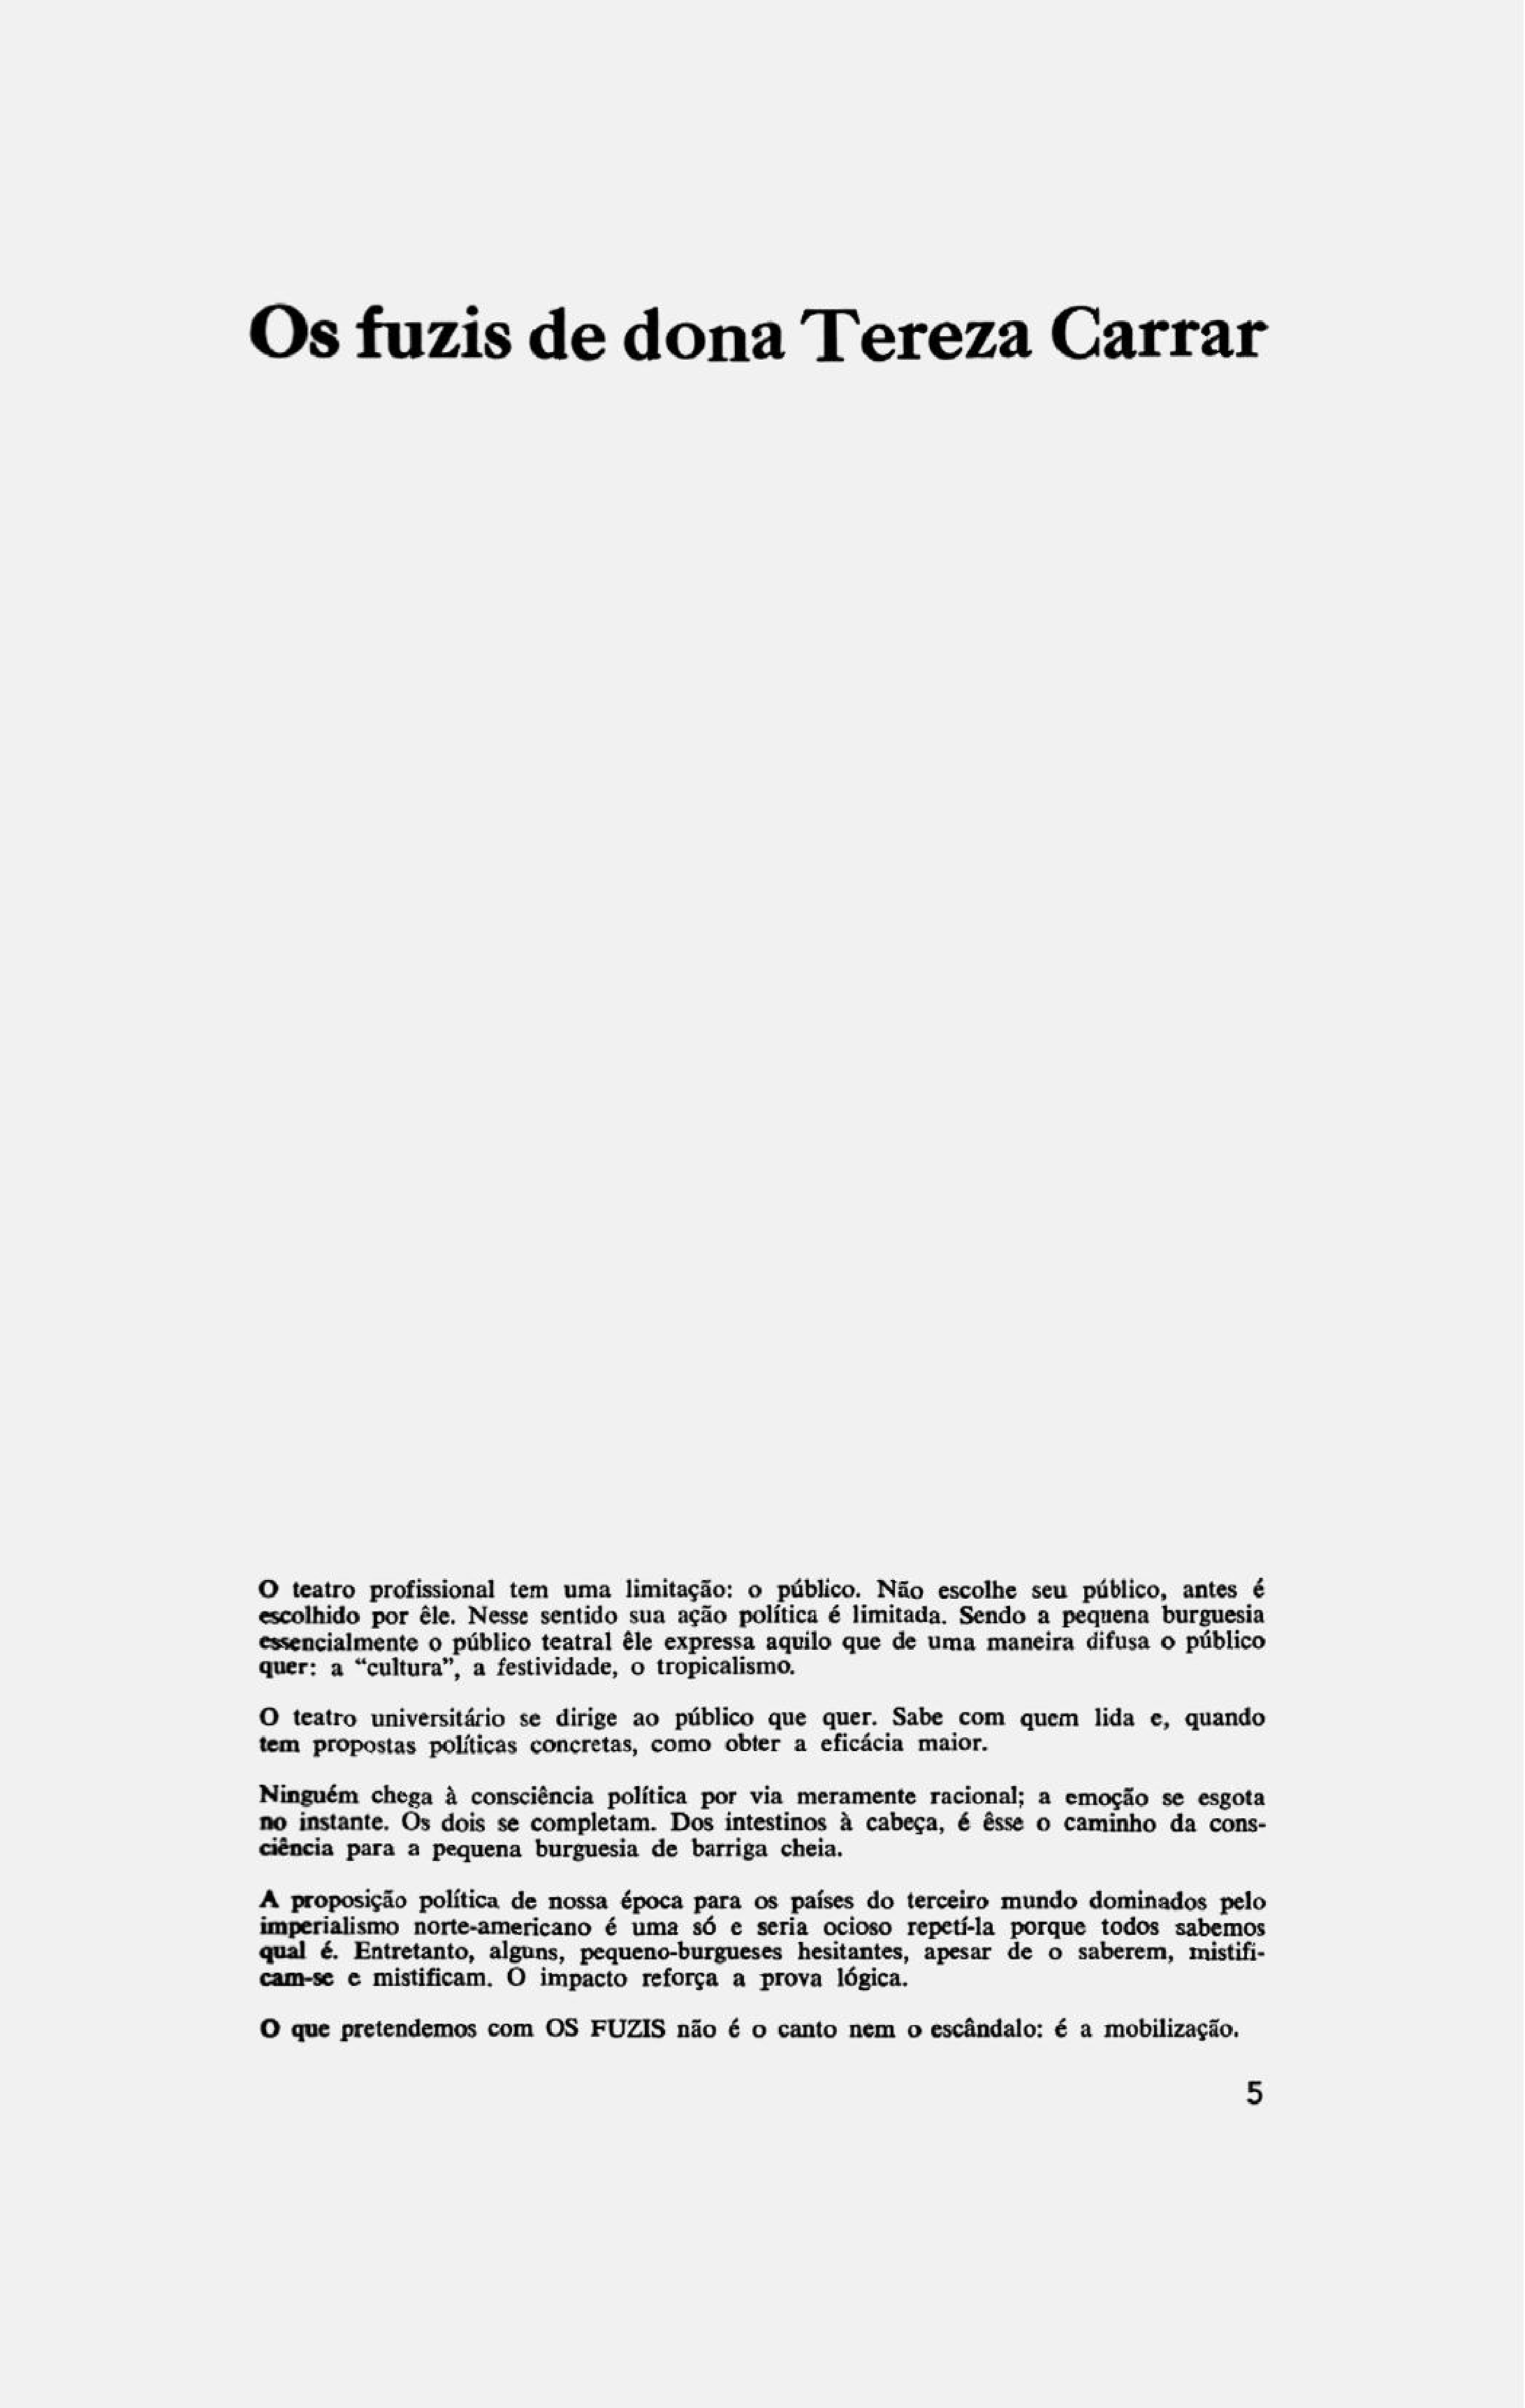
\includegraphics[width=\columnwidth]{./media/DOC3.pdf}

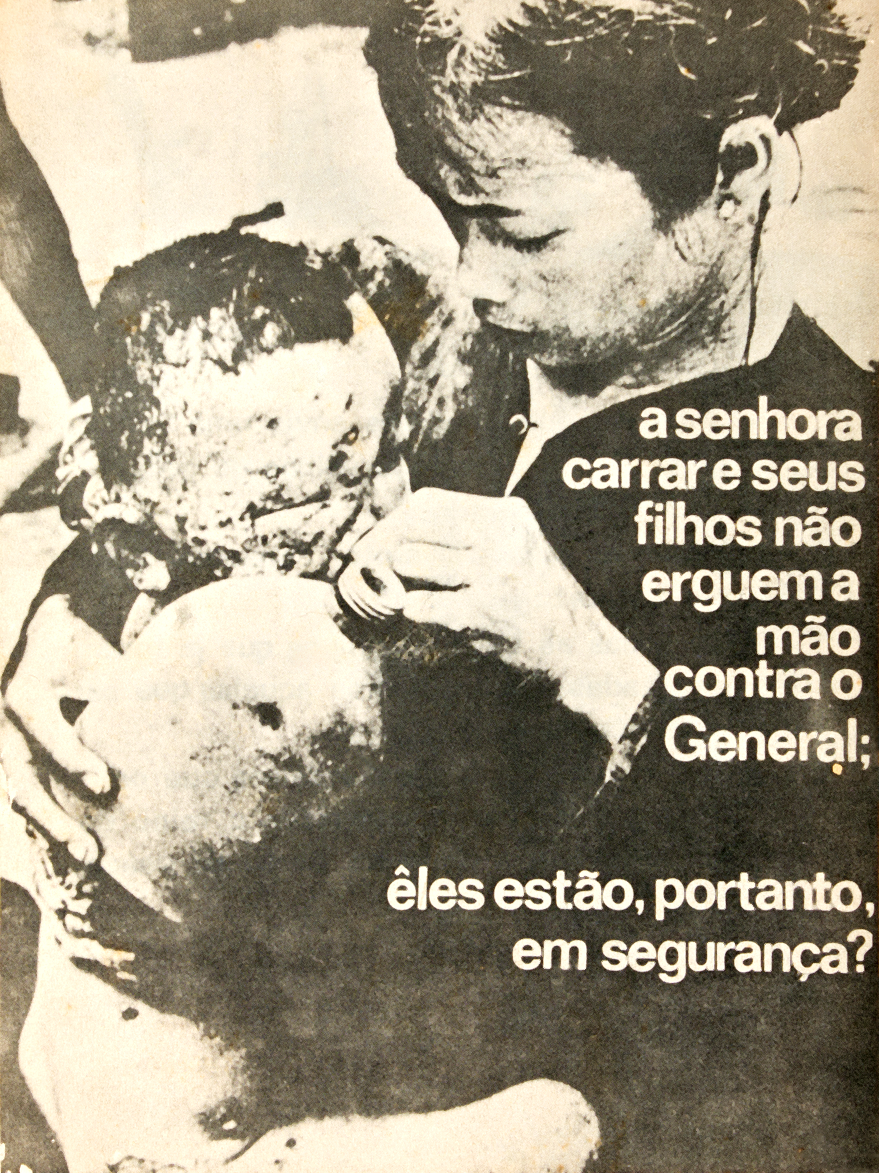
\includegraphics[width=\columnwidth]{./media/IMAGEM10.png}

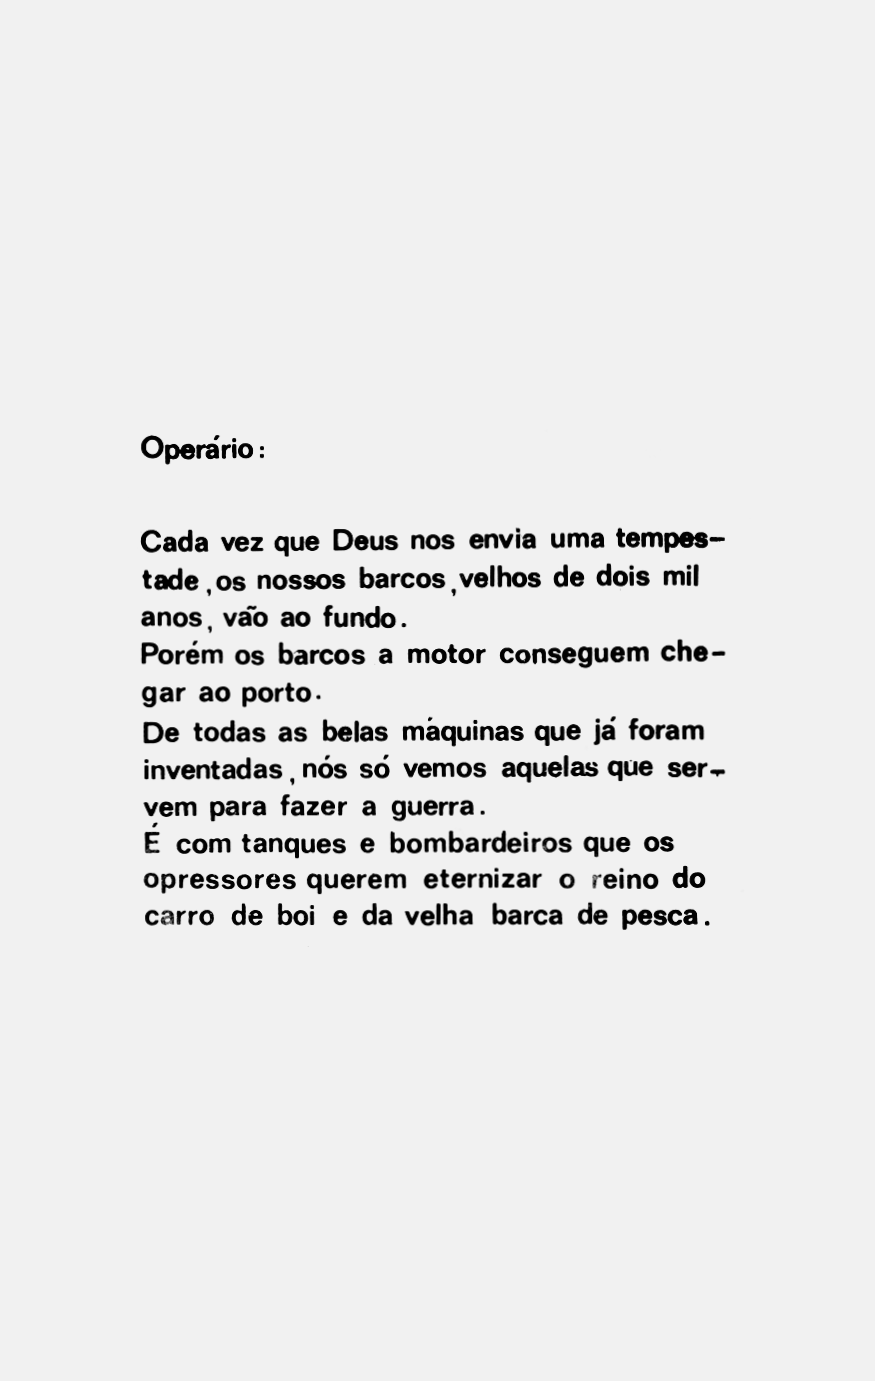
\includegraphics[width=\columnwidth]{./media/IMAGEM11.png}

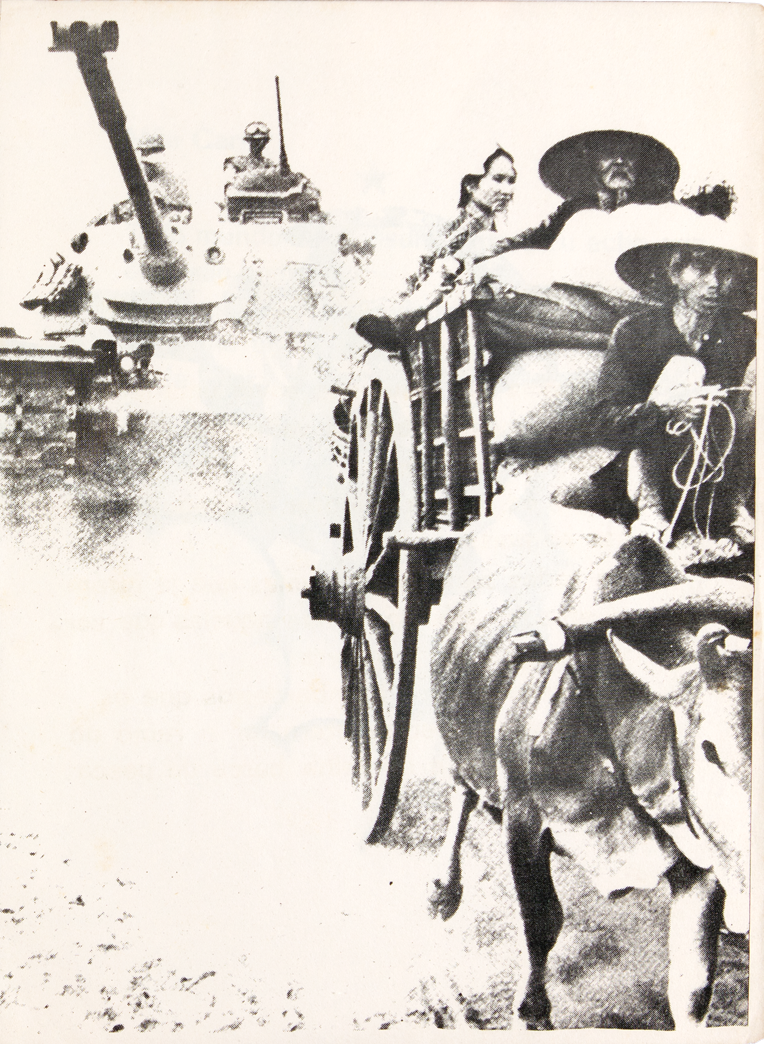
\includegraphics[width=\columnwidth]{./media/IMAGEM12.png}

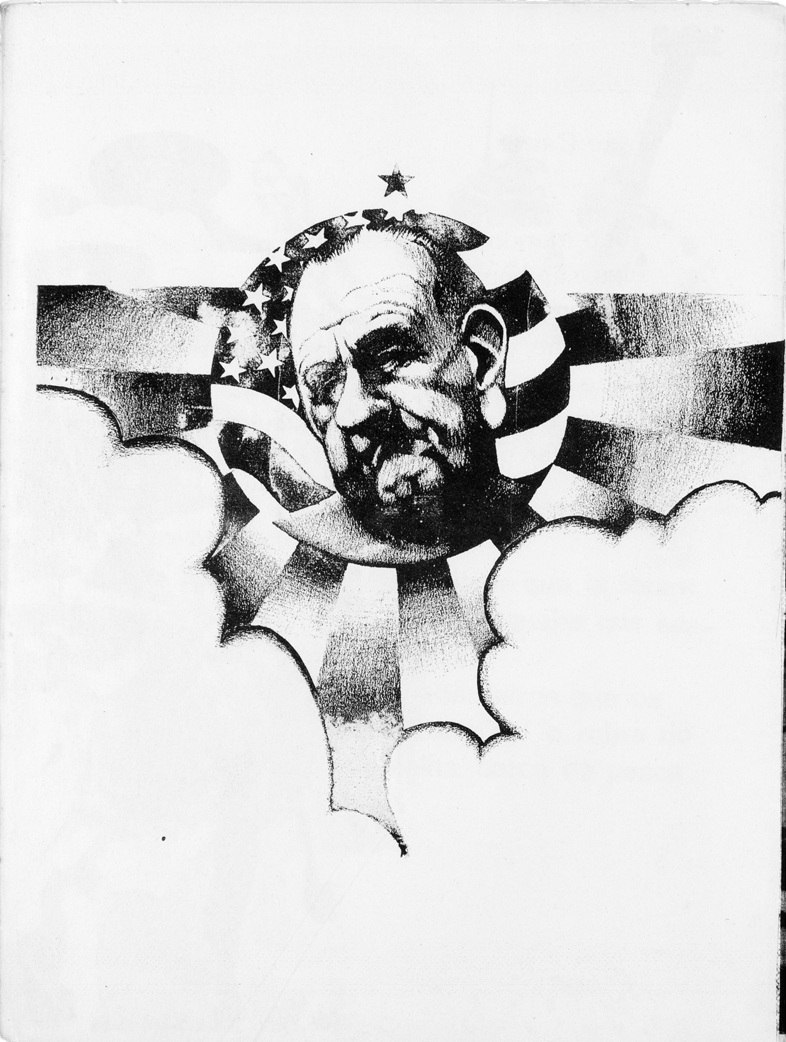
\includegraphics[width=\columnwidth]{./media/IMAGEM13.png}

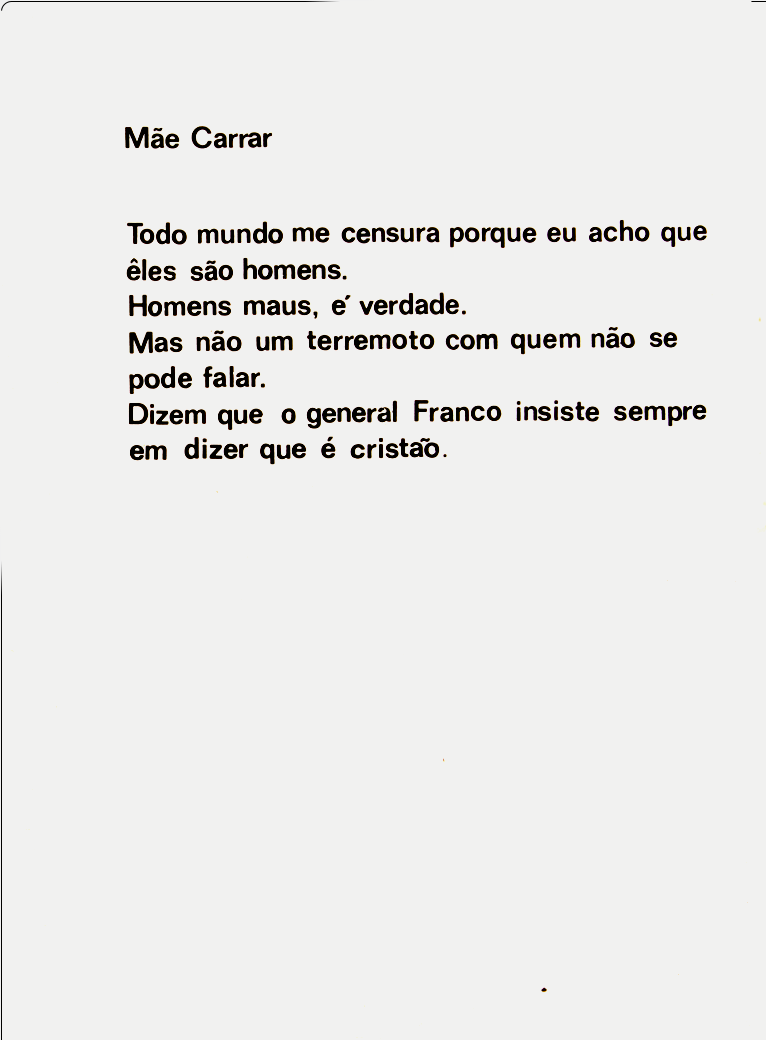
\includegraphics[width=\columnwidth]{./media/IMAGEM14.png}

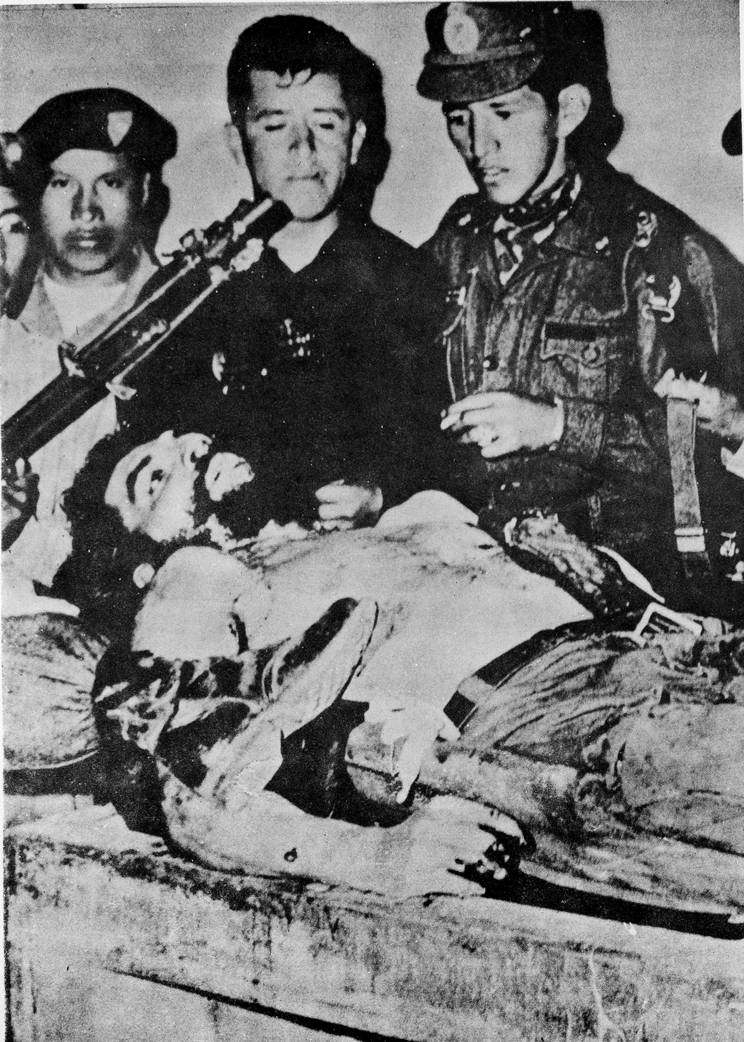
\includegraphics[width=\columnwidth]{./media/IMAGEM15.png}

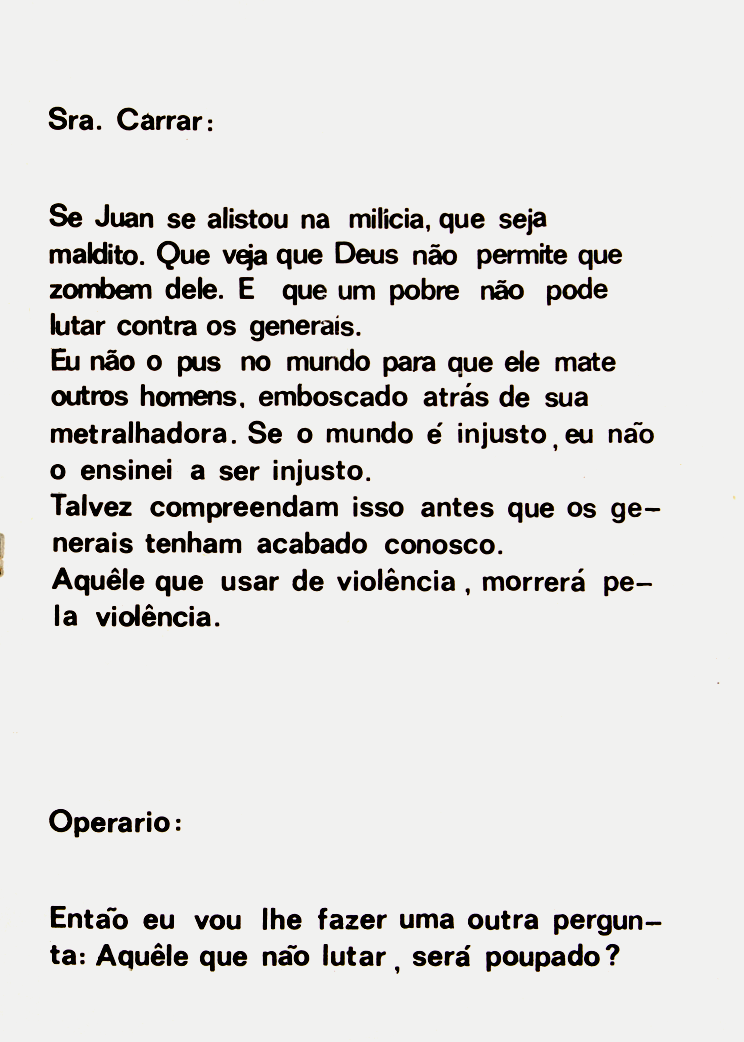
\includegraphics[width=\columnwidth]{./media/IMAGEM16.png}

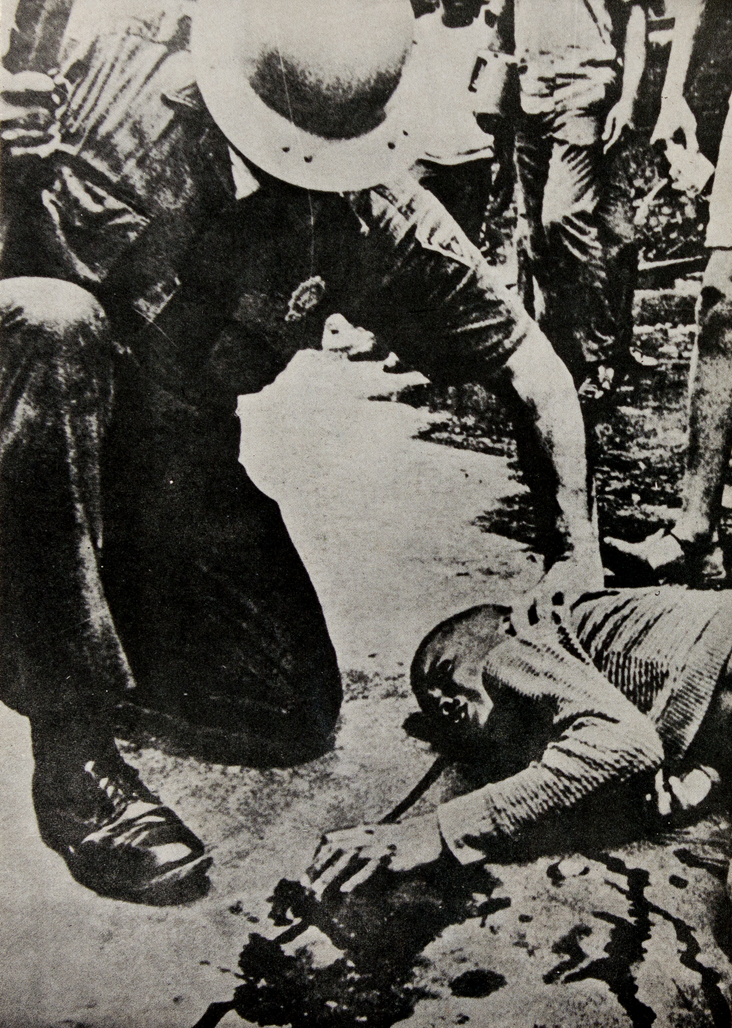
\includegraphics[width=\columnwidth]{./media/IMAGEM17.png}

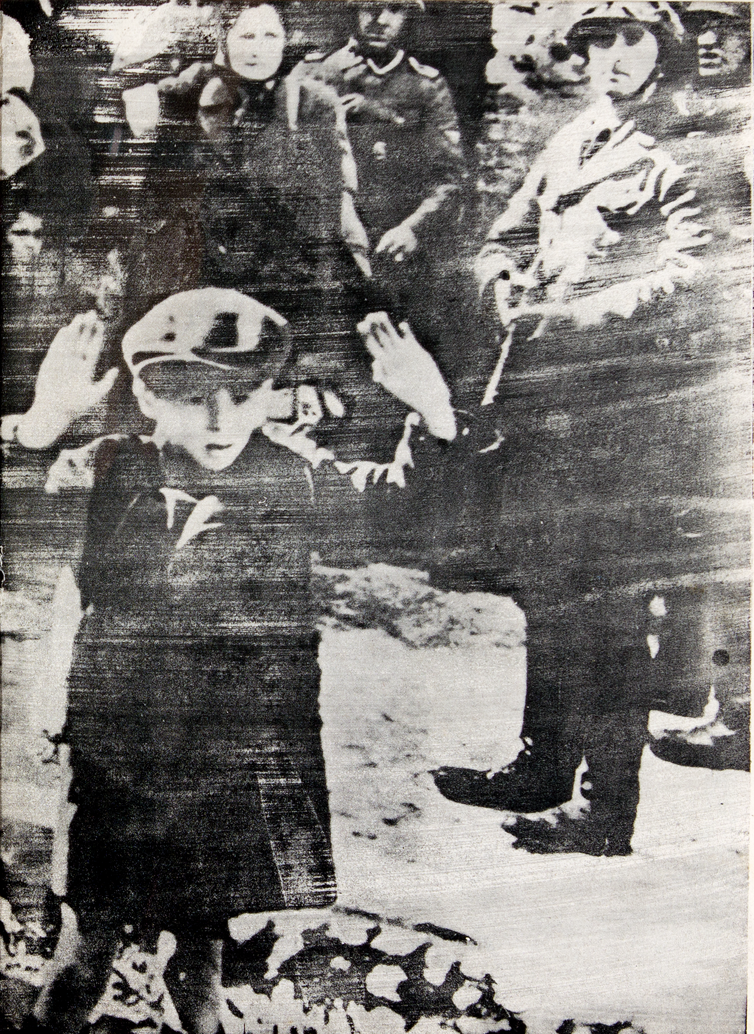
\includegraphics[width=\columnwidth]{./media/IMAGEM18.png}

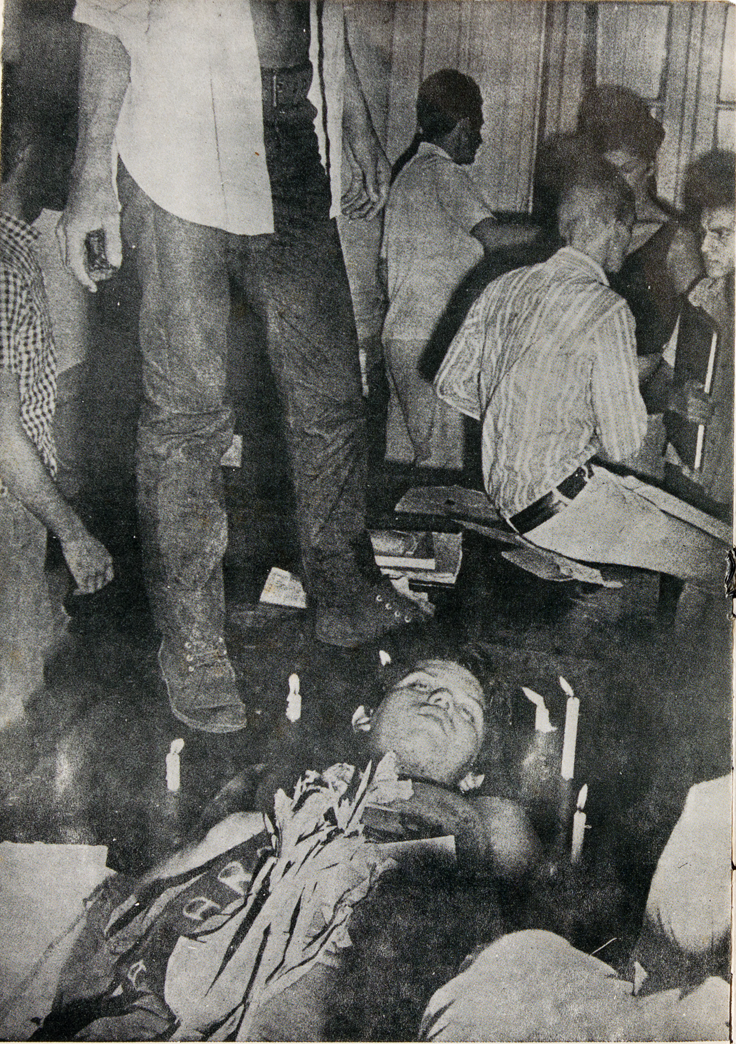
\includegraphics[width=\columnwidth]{./media/IMAGEM19.png}

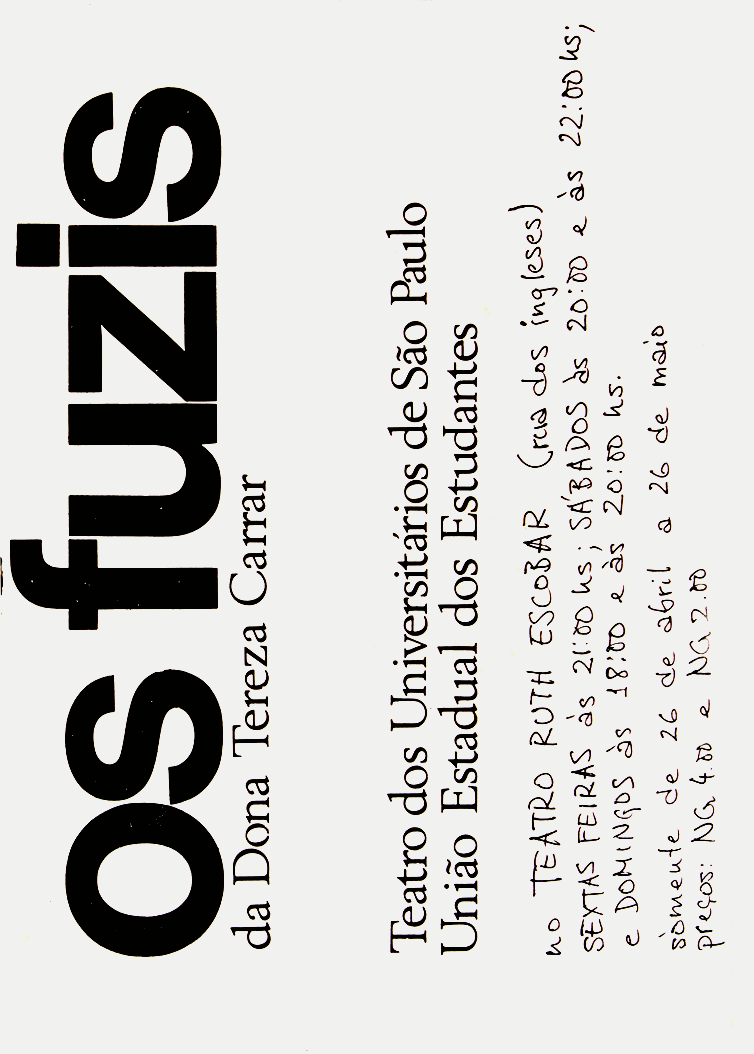
\includegraphics[width=\columnwidth]{./media/IMAGEM20.png}

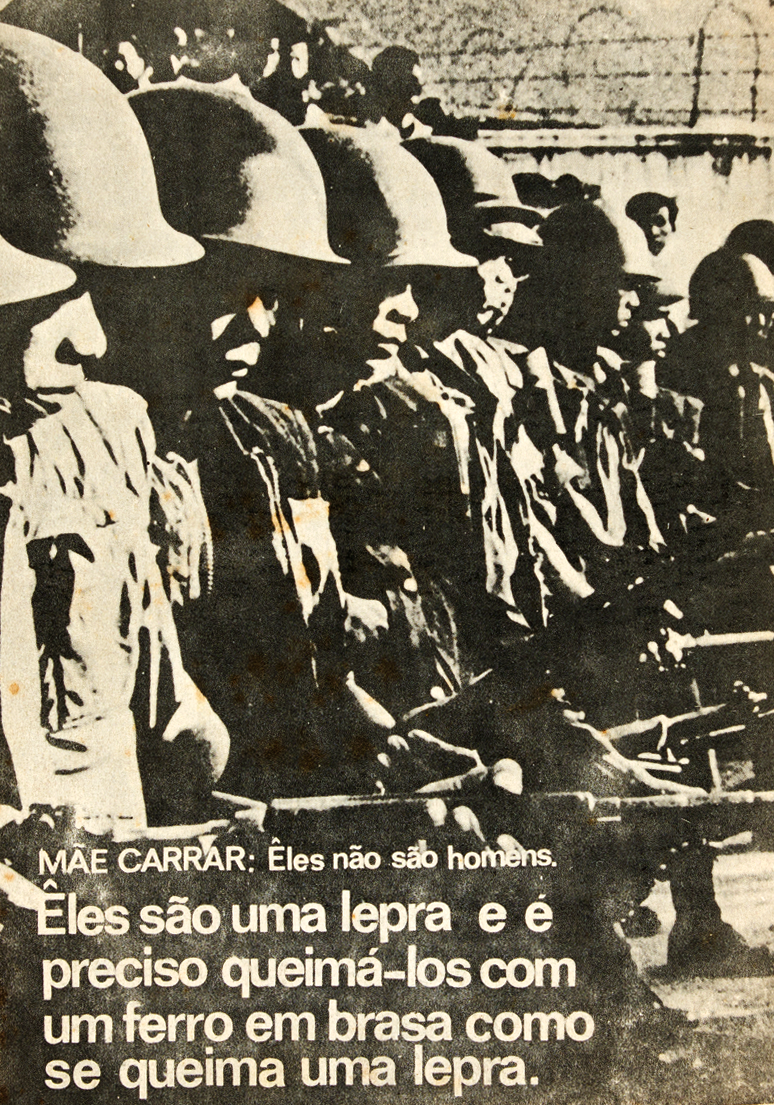
\includegraphics[width=\columnwidth]{./media/IMAGEM21.png}


\begin{figure}
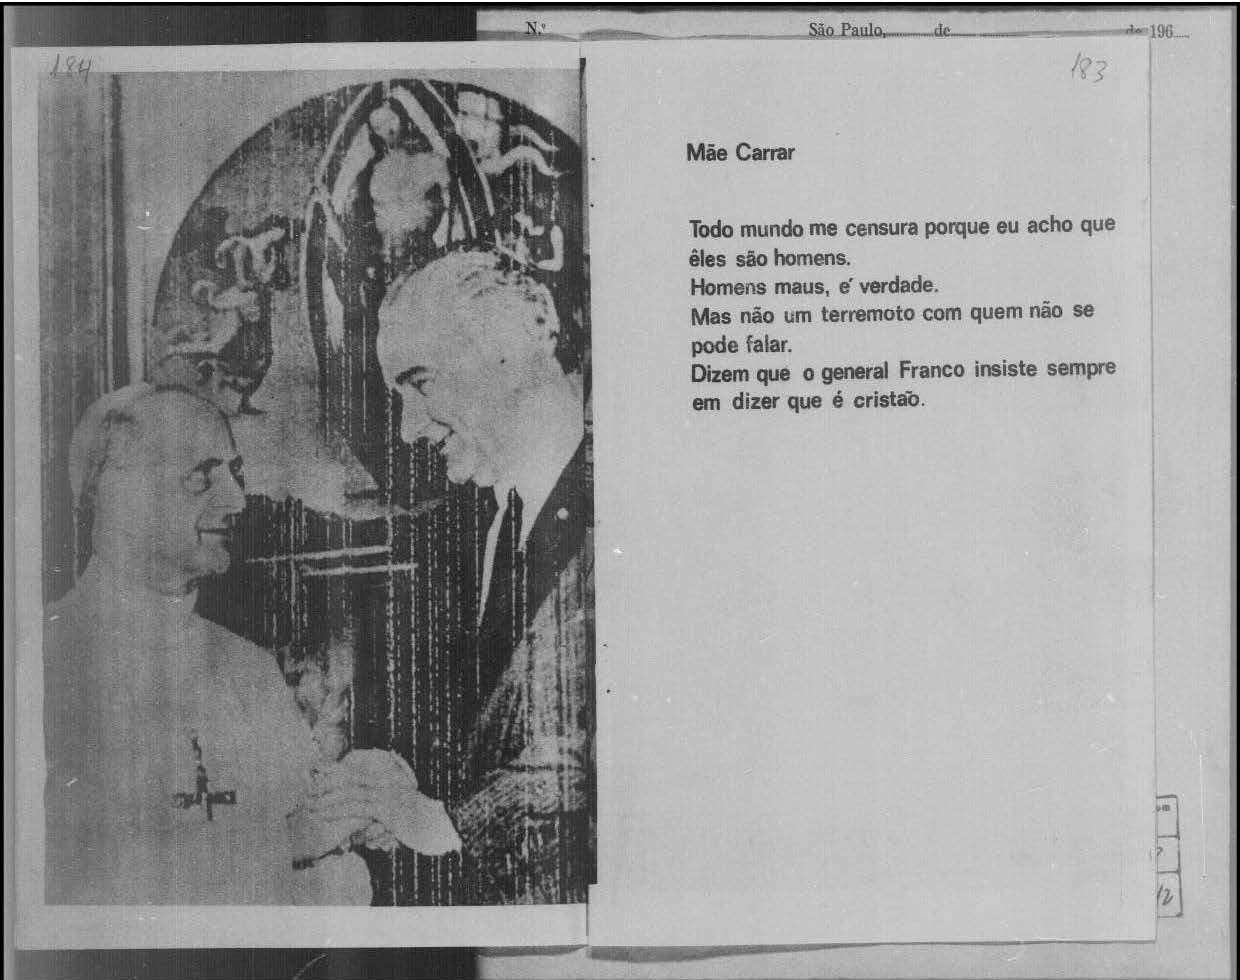
\includegraphics[width=\columnwidth]{./media/IMAGEM22.jpg}
\caption{Um
programa do espetáculo apreendido pela polícia política trazia essa
página, que não consta na versão do programa presente no Acervo Flávio
Império. Arquivo do Estado.}
\end{figure}

\begin{figure}
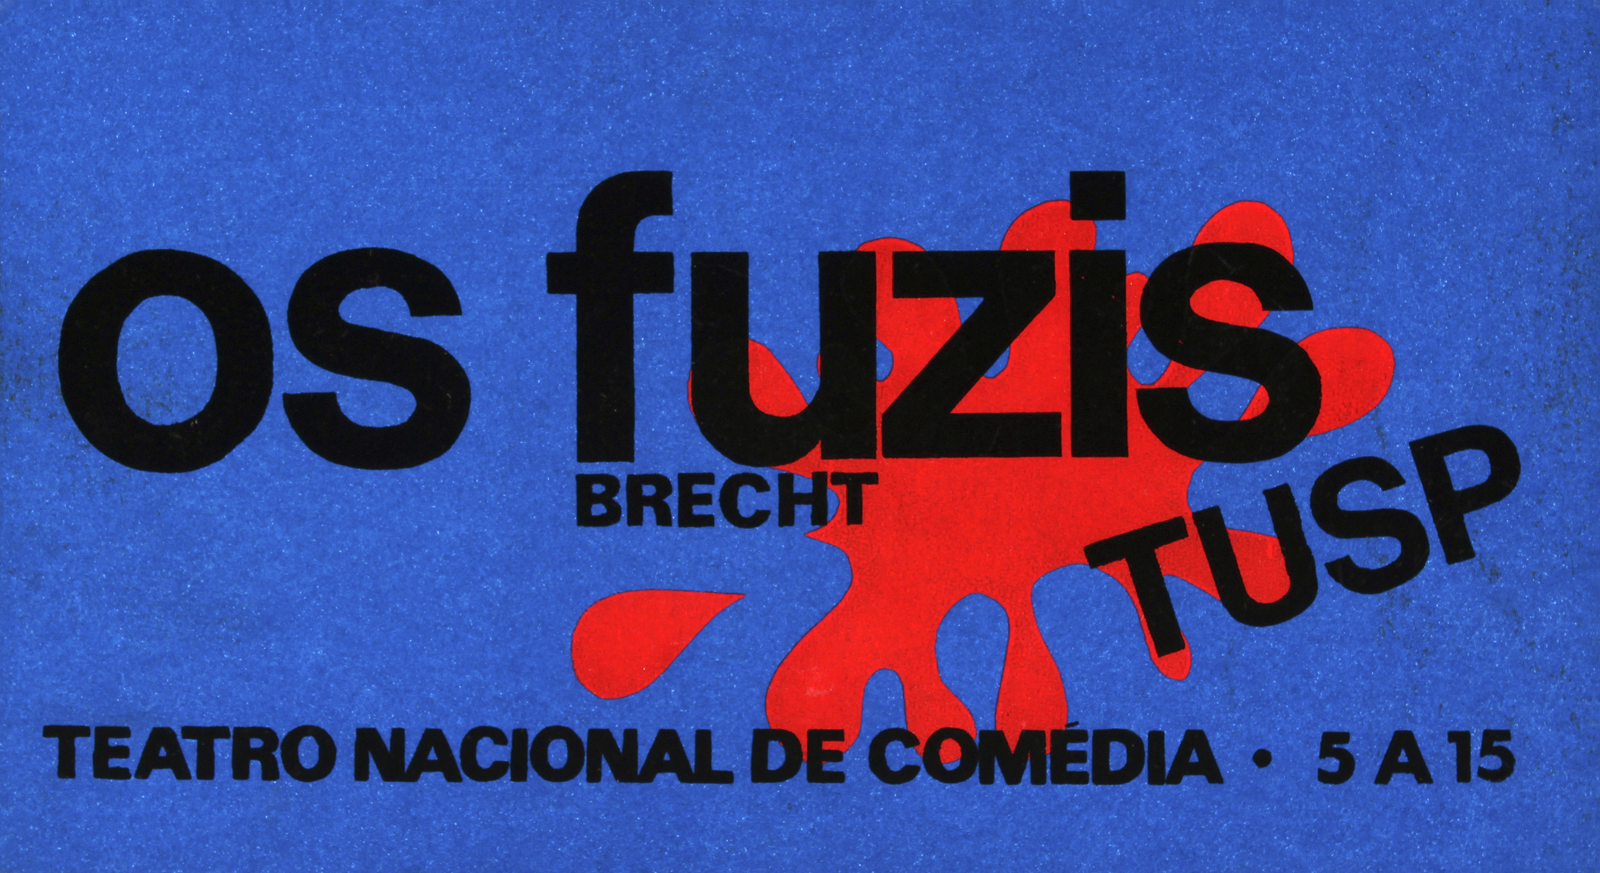
\includegraphics[width=\columnwidth]{./media/IMAGEM23.png}
\caption{Convite do espetáculo no Rio de Janeiro. Acervo Flávio Império.}
\end{figure}

\chapter{IMAGENS DE \textit{OS FUZIS}: PESQUISA DOS GESTOS}

Quando o TUSP realizava os últimos ensaios de \textit{Os fuzis}, no início
de 1968, Victor Knoll, professor de Estética na Faculdade de Filosofia,
registrou, em mais de uma sessão fotográfica, o trabalho do grupo. Suas
imagens, somadas a algumas outras que circularam entre os jornais da
época e a \textit{frames} de um pequeno trecho gravado em vídeo no Festival
de Nancy de 1969, permitem que se veja algumas das formas com que o TUSP
procurou interpretar ou deslocar os sentidos do material do texto de
Brecht.

Existe um artigo do crítico Roland Barthes, escrito para a revista
\textit{Théâtre Populaire}, em que ele analisa a montagem de \textit{Mãe
Coragem} apresentada pelo Berliner Ensemble em Paris, em 1957, a partir
de fotos de Roger Pic. Intitulado “Sete Fotos-Modelo de \textit{Mãe
Coragem}”, ali, Barthes observa:

\begin{quote}
Aquilo que a fotografia revela é exatamente o que é ofuscado pela
representação, o detalhe. Ora, o detalhe é o lugar privilegiado da
significação, e é porque o teatro de Brecht é um teatro da significação
que o detalhe nele é tão importante.\footnote{Publicado em \textit{Escritos
  sobre teatro} (São Paulo: Martins Fontes, p. 239-260).}
\end{quote}

Procuramos seguir seu exemplo e destacar, nos comentários que se seguem,
alguns dos detalhes do espetáculo do TUSP em seu esforço de atualizar a
peça de Brecht e torná-la viva. Registramos, ao lado deles, o uso de
colagens, forma que dialoga com tendências artísticas do tempo, como a
Tropicália, e a opção por uma teatralidade exposta e baseada no
contraste com imagens realistas e dramáticas. Descrevemos, ainda, formas
de uma “atitude de guerrilha” que extravasa do assunto da peça de Brecht
para a relação com a plateia universitária.

\begin{figure}
\includegraphics[width=\columnwidth]{./media/IMAGEM24.png}
\caption{Fotógrafo: L. Pinto. 1968. Acervo Última Hora. Arquivo Público do Estado de São Paulo.}
\end{figure}

\begin{itemize}
\item
  Ícones mortuários
\end{itemize}

Na peça de Brecht, a ação se passa na sala de uma casa de pescadores.
Paredes caiadas, um crucifixo preto. Há uma janela, de onde a Mãe Carrar
observa seu filho, Juan. Ele pesca ao longe, no mar. Ela assa o pão em
um forno de barro. José, seu outro filho, entalha um artefato pesqueiro.
Canhões são escutados ao longe.

Flávio Império constrói uma sala sem paredes. O espaço da família é
indicado pelo palco de tábuas largas, levemente inclinado. Um forno de
assar pão está perto de uma mesa rústica de madeira. Pedaços da rede de
pesca indicam o ofício familiar. Ao fundo, um crucifixo suspenso,
desproporcional.

Anos antes, na montagem do Arena de 1962, com direção de José Renato, o
cenógrafo Flávio Império se manteve mais próximo do realismo dramático
do original. Agora seu espaço é narrativo: colado ao tablado, no fundo,
se ergue uma trincheira com sacos de areia, como a dizer “estamos em
guerra”. 1968, o ano eternizado na imagem das \textit{barricadas do
desejo}\footnote{A expressão dá nome ao livro da filósofa Olgária Matos,
  \textit{Paris 1968: as barricadas do desejo} (São Paulo: Brasiliense,
  1998).}.

Um estandarte flutua no alto com um tecido manchado de vermelho,
sugerindo sangue, próximo à plateia. Nele se lê: “Guanabara, 28 de março
de 1968”. O local e data são os do assassinato do estudante
secundarista, Edson Luís de Lima Souto, morto em um confronto com a
polícia na ocupação do restaurante universitário Calabouço, no Rio de
Janeiro. A memória de sua morte recente diz respeito a todos os
artistas, num ano em que os estudantes ocuparam o centro da cidade de
São paulo, a Faculdade de Filosofia, e enfrentaram o Comando de Caça aos
Comunistas, na Batalha da Maria Antonia, quando a faculdade foi
incendiada e foi assassinado o também secundarista José Carlos
Guimarães.

No conjunto cenográfico, a guerra iminente: o tablado conduz à
trincheira. A nota dissonante é a enorme cruz. Anuncia a aliança entre a
Igreja e o fascismo apontada no texto de Brecht, com uma ambiguidade
nova. O cuidado com que foi construída por Flávio Império, a partir de
objetos plásticos encontrados em armarinhos pelo centro da cidade,
contém também outra força, a da fabricação industrial em série, a dos
restos do mundo petroquímico que apoiava a contrarrevolução brasileira.
É um objeto conforme o imaginário tropicalista, síntese do atraso
conservador e do avanço mercantil. Sua composição sugere ainda uma coroa
de flores, dessas que se enviam aos velórios. Está à mesma altura do
estandarte mortuário de Edson Luís, segundo uma linha diagonal
imaginária. A religião dos fascistas está decorada pela divindade
cambiante do consumo, com suas quinquilharias multicoloridas de
barroquismo mercantil. A perspectiva da morte sobrevoa a cena.

\begin{figure}

\includegraphics[width=\columnwidth]{./media/IMAGEM25.png}
\caption{Bety Chachamovitz como Senhora Carrar. 1968. Fotógrafo: Victor Knoll.
Acervo pessoal.}
\end{figure}

\begin{itemize}
\item
  Rede trágica
\end{itemize}

Quando as portas do teatro se abrem, Tereza Carrar e seu filho mais
jovem, José realizam pequenos gestos de trabalho. Tereza desembaraça ou
costura a rede de pesca. Ela observa - com o olho da alma - a morte do
marido na frente de batalha, de passado recente. A posição é reflexiva,
como sugere o cotovelo apoiado no joelho, e o tronco tombado à frente.
Ela fará de tudo para manter a família afastada da luta, está empenhada
em que a guerra - que ela um dia apoiou - não leve seus filhos.

A rede de pesca envolve seus pés e joelhos. Caso se erga, para levar a
massa de pão ao forno, ou para ver o barco do filho que pesca no mar, ao
largo, terá dificuldades. A rede a envolve. A consciência cindida entre
o desejo de preservação dos filhos e a pressão da comunidade para que
participe da luta, cria uma estaticidade que não é paralisia, em meio à
tragicidade alegorizada no enredamento do corpo. Como outras mães de
Brecht, seu esforço resistente de não deixar o filho partir para a
guerra se mostrará como parte de uma catástrofe maior.

O público da montagem do TUSP é recebido no teatro por uma gravação
sonora, vinda dos alto-falantes. Em lugar do som dos canhões da Guerra
Civil Espanhola proposto por Brecht, ouvimos um discurso científico
sobre o \textit{napalm}, enunciado em tom monótono. Os espectadores são
informados sobre a composição e os efeitos nefastos das bombas químicas
usadas pelos Estados Unidos na Guerra do Vietnã. Antes que toda a gente
esteja sentada, têm início a projeção em \textit{slide} pelas superfícies
do espaço cênico ou pelas paredes da sala. Nas imagens brutais, ao som
do discurso, são justapostas duas guerras irracionais de épocas
diferentes, com suas ciências próprias, uma de tipo fascista, outra
justificada pela razão liberal.

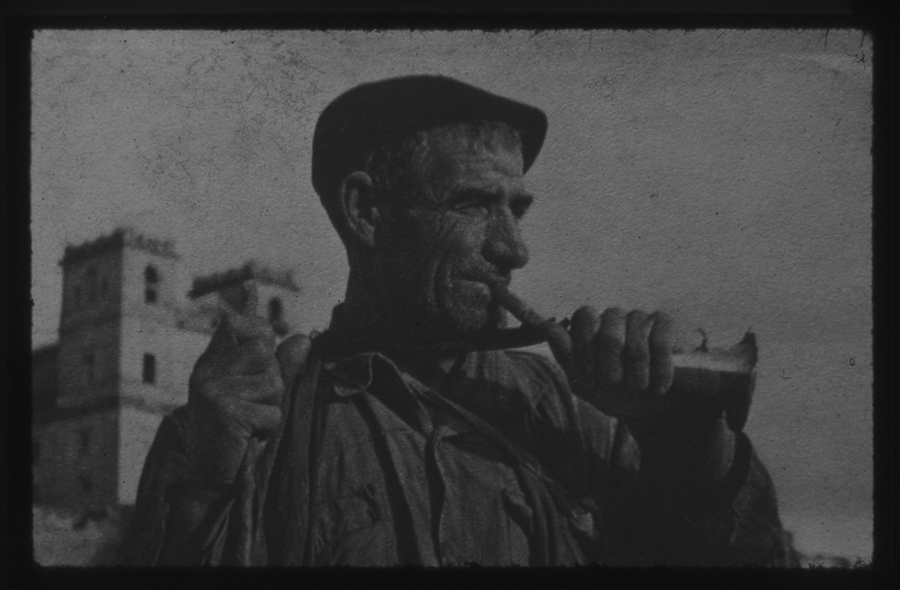
\includegraphics[width=\columnwidth]{media/IMAGEM26.jpg}
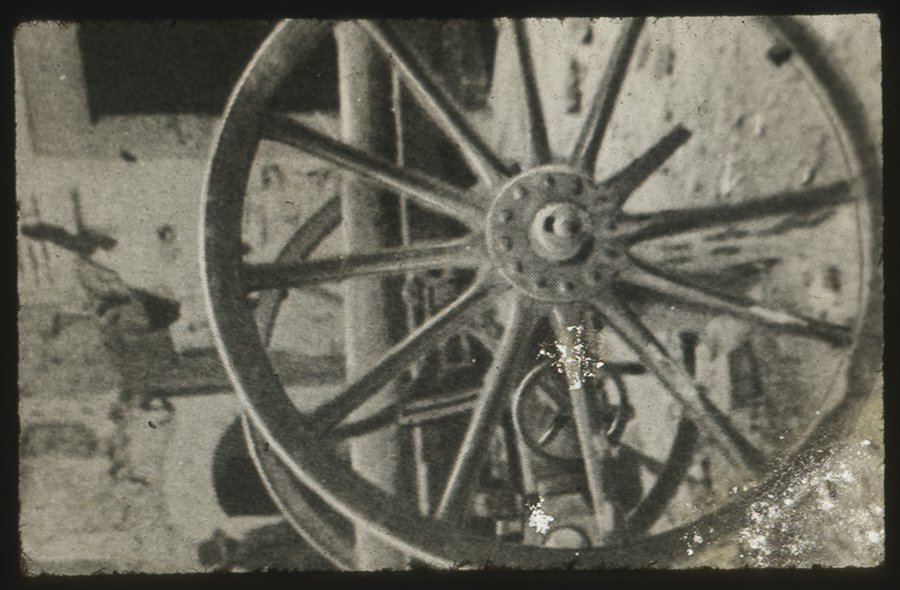
\includegraphics[width=\columnwidth]{media/IMAGEM27.jpg}
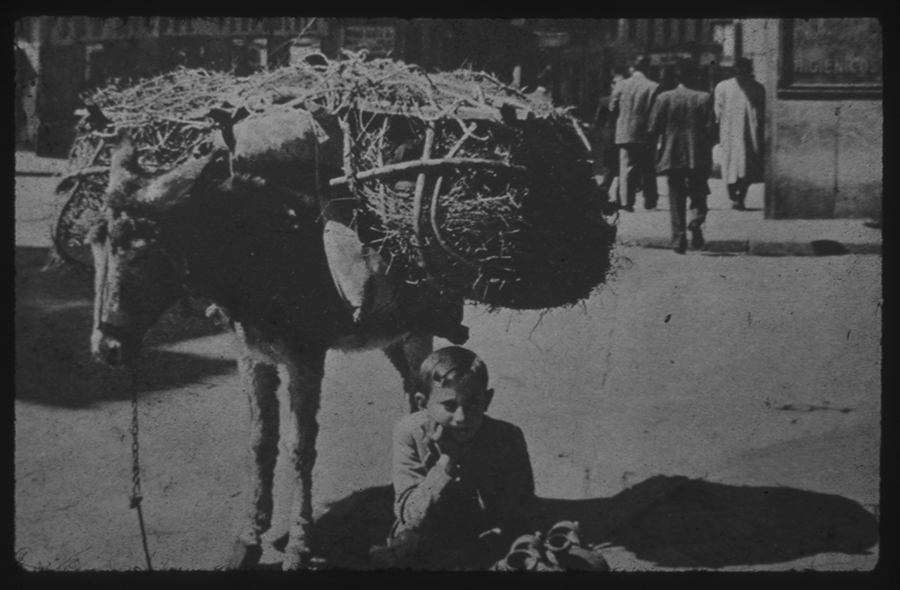
\includegraphics[width=\columnwidth]{media/IMAGEM28.jpg}
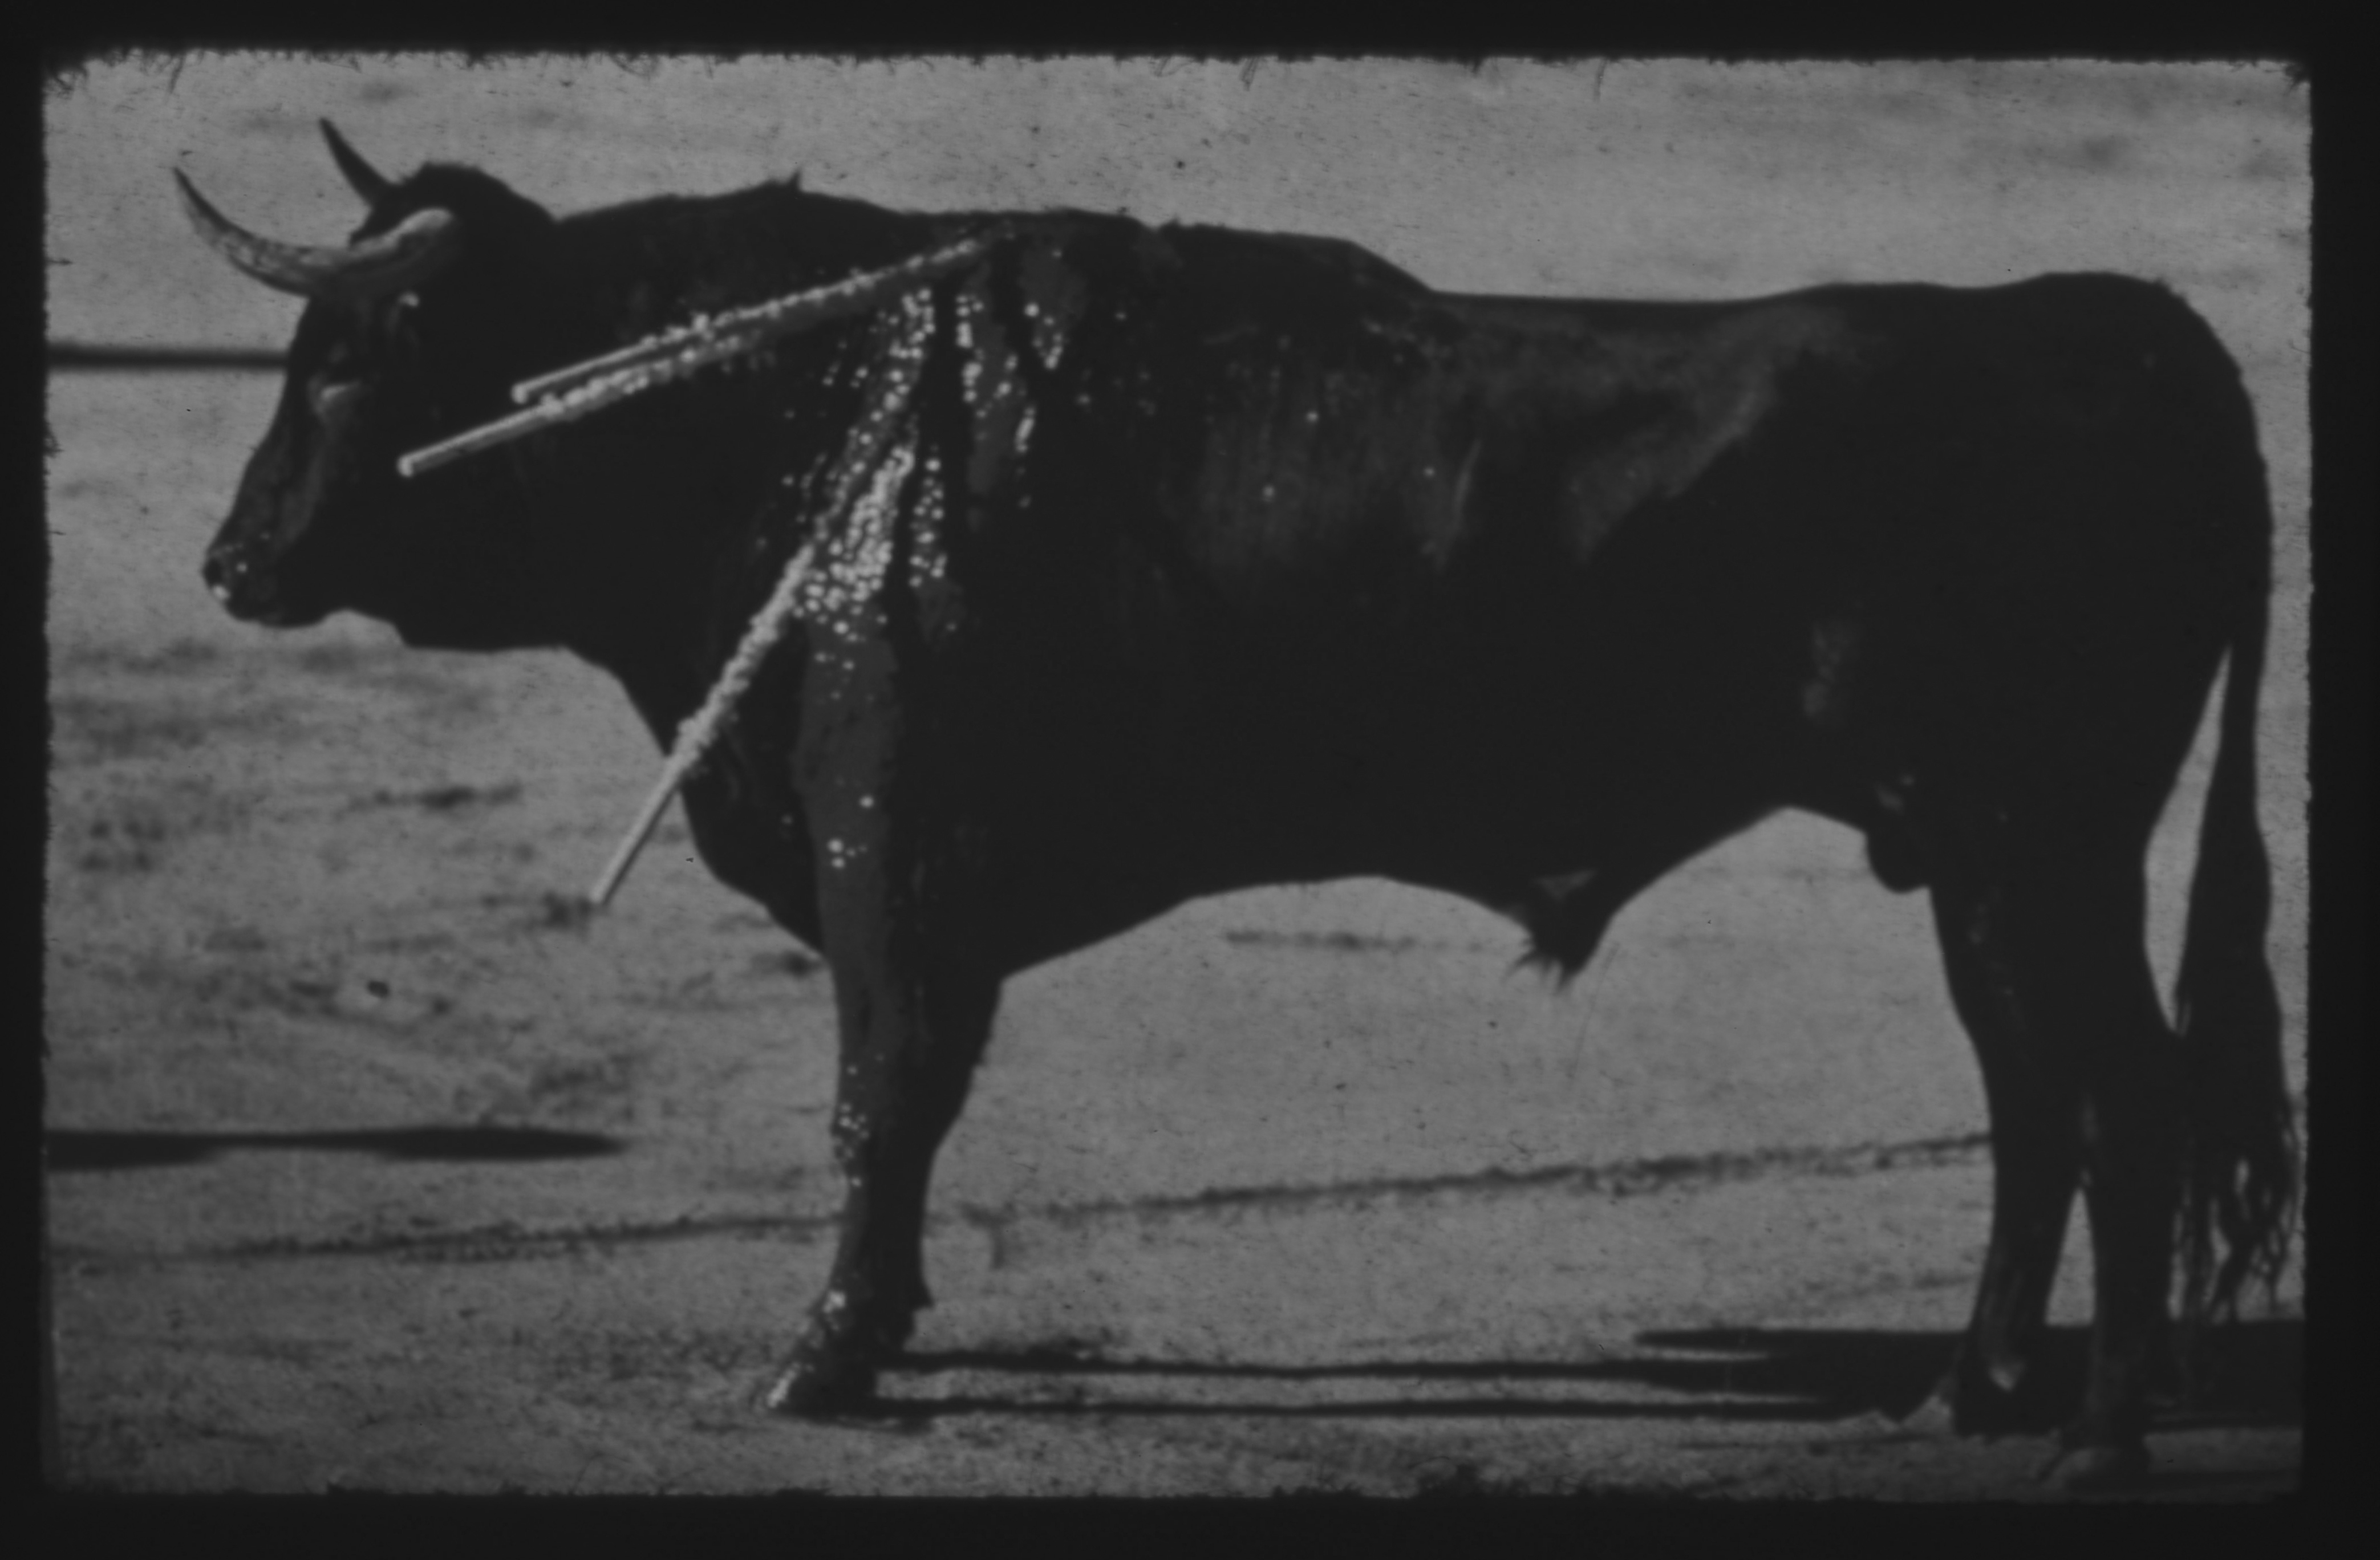
\includegraphics[width=\columnwidth]{media/IMAGEM29.jpg}
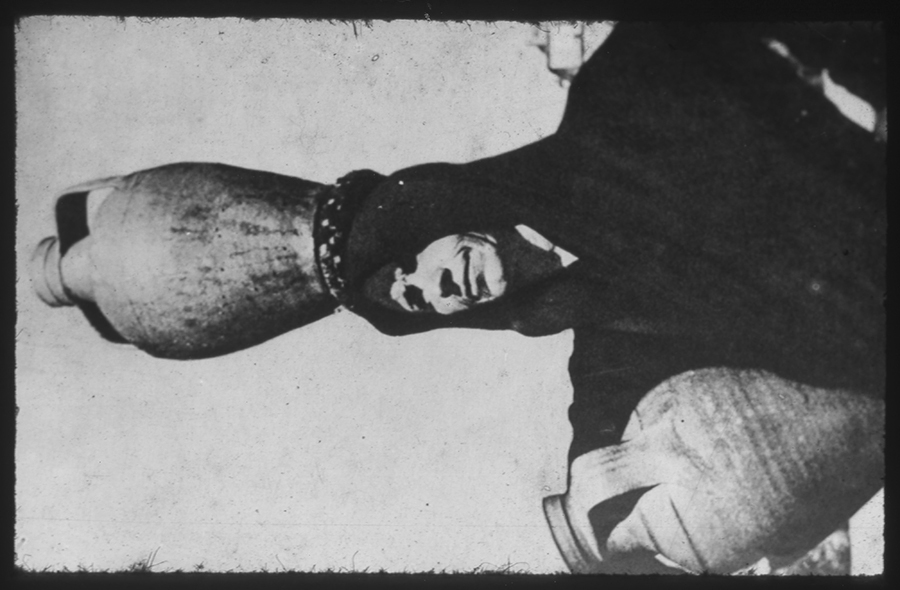
\includegraphics[width=\columnwidth]{media/IMAGEM30.jpg}
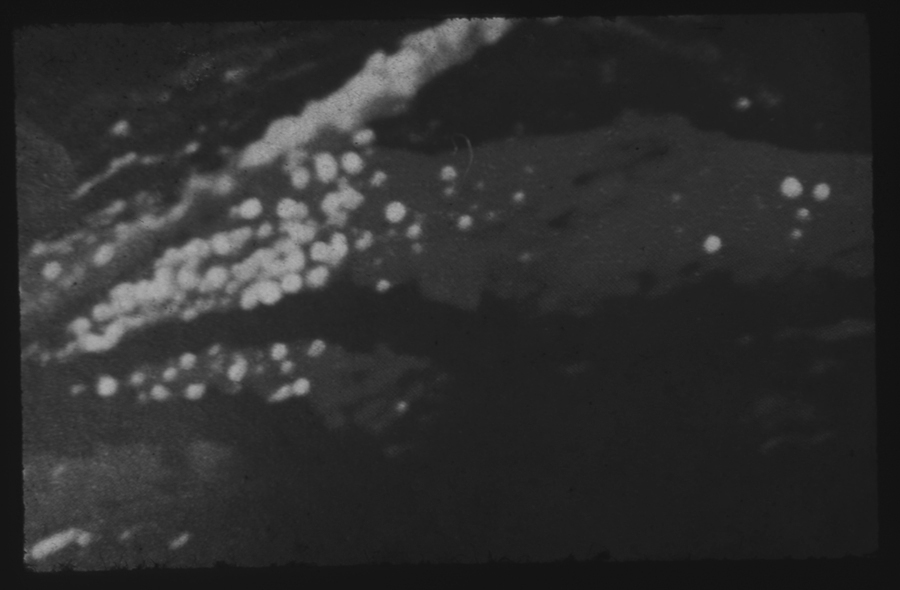
\includegraphics[width=\columnwidth]{media/IMAGEM31.jpg}
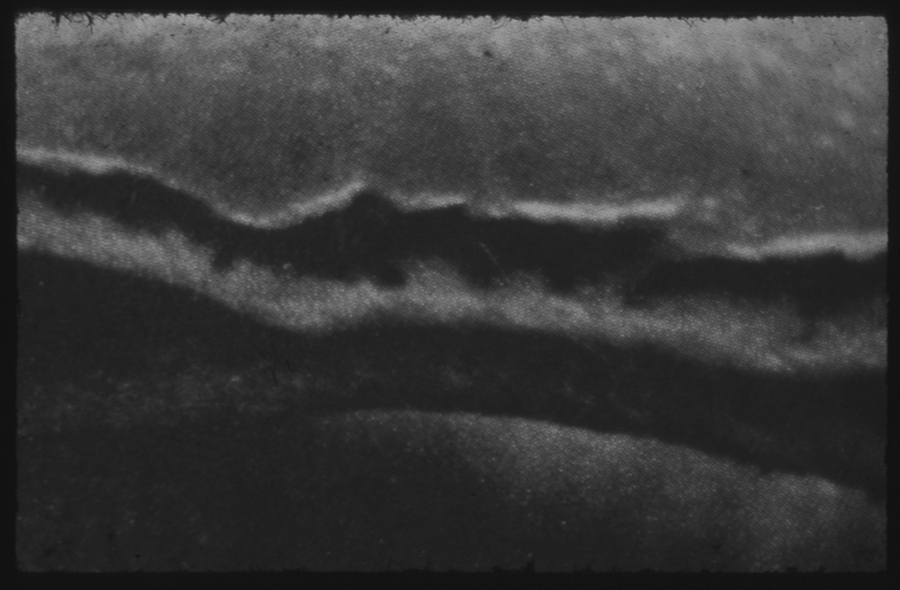
\includegraphics[width=\columnwidth]{media/IMAGEM32.jpg}
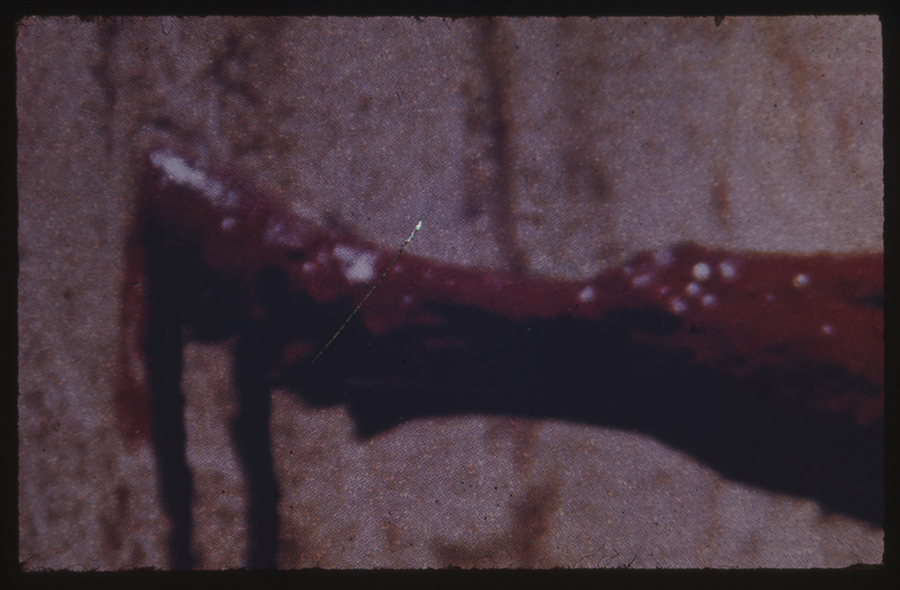
\includegraphics[width=\columnwidth]{media/IMAGEM33.jpg}
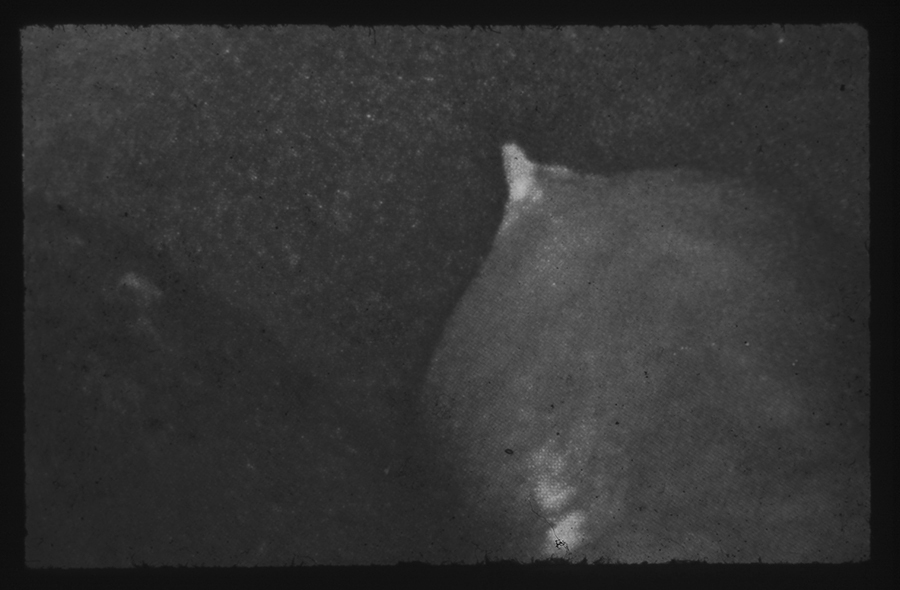
\includegraphics[width=\columnwidth]{media/IMAGEM34.jpg}
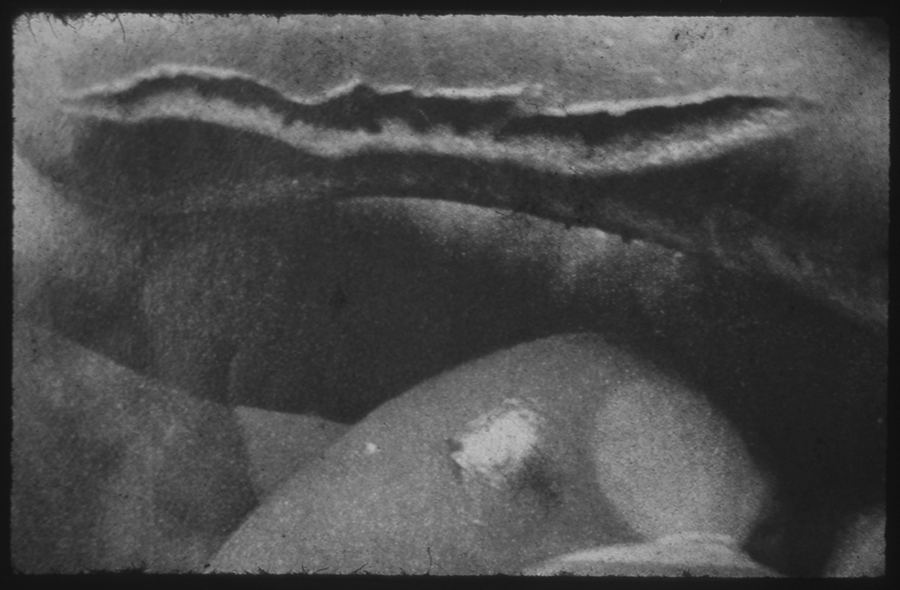
\includegraphics[width=\columnwidth]{media/IMAGEM35.jpg}
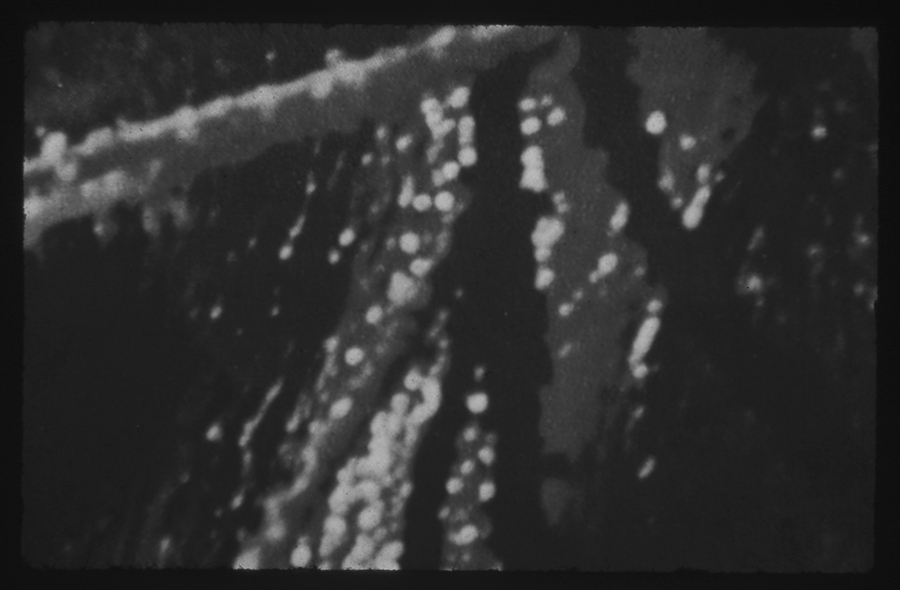
\includegraphics[width=\columnwidth]{media/IMAGEM36.jpg}
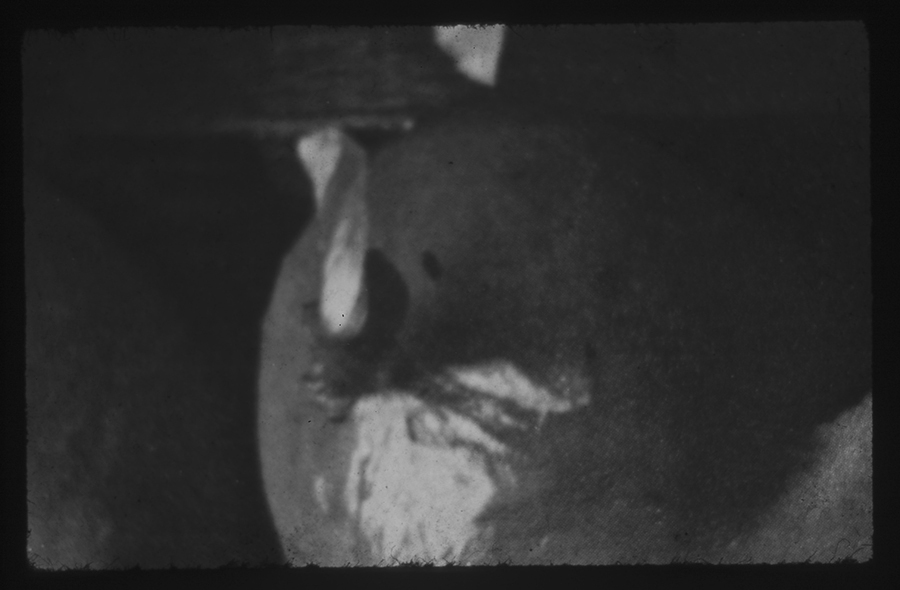
\includegraphics[width=\columnwidth]{media/IMAGEM37.jpg}

\textit{Slides}. Acervo Flávio Império.

\begin{itemize}
\item
  Sangue audiovisual
\end{itemize}

O áudio sobre o \textit{napalm} é substituído pela gravação de uma
conferência didática sobre a história da Guerra Civil Espanhola
inspirada pelo livro de Hugh Thomas, recém traduzido no
Brasil.\footnote{\textit{A Guerra Civil Espanhola} (Rio de Janeiro:
  Civilização Brasileira, 1964).} Começamos a ser levados ao tempo da
peça de Brecht. O tecido ensanguentado com o local e data do assassinato
de Edson Luís, entrentanto, paira iluminado, e é sustentado por um
fuzil. A bandeira nos acompanha como um lembrete sobre a violência do
país atual. \footnote{Como o espetáculo era permeável a transformações
  durante as temporadas e conforme o momento que se vivia (e por vezes,
  a pressão da censura), a referência ao assassinato de Edson Luís foi
  intensificada na temporada carioca, em julho de 1968. As apresentações
  no Rio se iniciaram no dia seguinte à Passeata dos 50 Mil, a última da
  série de grandes manifestações estudantis.}

Os \textit{slides} agora exibem imagens da Espanha, de pequenos vilarejos e
uma longa sequência de uma tourada. Um touro embandeirado sangra. A
projeção, elaborada por Claudio Tozzi, em parceria com Flavio Império,
não é linear. Em rápidos \textit{flashes} aparecem também retratos
coloridos de Che Guevara que Tozzi produzia desde 1967, ano do
assassinato do guerrilheiro. As imagens já tinham acompanhado o TUSP em
exposições feitas durante as apresentações de \textit{A exceção e a regra},
e agora voltam à cena. Vietnã, Bolívia, Espanha, Brasil: a guerrilha em
meio ao sangue.

Já se passaram cerca de 20 minutos desde a entrada do público na sala de
espetáculos. O tom monótono e cientificista das gravações, inspirado
pela abordagem de \textit{O interrogatório} de Peter Weiss, sugere a
normalização do horror. A sequência dos \textit{slides} culmina na foto de
uma salsicha. Acordes \textit{jazzísticos} de Dave Brubeck comentam a
mutação do touro em carne industrializada em tom de escárnio, como
anunciando que a encenação não se restringirá à fábula dramática. Há
sangue de guerra na produção mercantil.

\begin{figure}
\includegraphics[width=\columnwidth]{./media/IMAGEM38.png}
\caption{Bety Chachamovitz como Senhora Carrar. 1968. Fotógrafo: Victor Knoll.
Acervo pessoal}
\end{figure}

\begin{itemize}
\item
  O mar dos pobres
\end{itemize}

O diálogo entre mãe e filho se inicia após o prólogo audiovisual, e
expõe o conflito central da peça. José, o filho mais novo, insiste na
possibilidade de contribuírem na resistência, sua mãe defende que se
mantenham neutros. O tema da participação provém de um olhar de ambos
para fora de cena, para algo que o drama sozinho não enxerga:

MÃE - Ainda está vendo o barco de Juan?

FILHO - Estou.

MÃE - E a lanterna continua acesa?

FILHO - Continua. {[}...{]} Estou com fome.

MÃE - E ainda não quer que seu irmão vá pescar!

FILHO - Isso é uma coisa que eu posso fazer. O lugar de Juan é na linha
de frente.

{[}...{]}

MÃE - Nós não somos revoltosos e não estamos fazendo frente a ninguém.
Se dependesse de vocês, talvez fizéssemos: você e seu irmão são
irresponsáveis por natureza. Nisso saíram a seu pai, e talvez eu nem
gostasse que fossem diferentes. Mas o que está aí não é brincadeira: não
escutam os canhões deles? Nós somos gente pobre, e gente pobre não pode
meter-se em guerra.\footnote{Os trechos aqui reproduzidos foram
  extraídos da tradução de Antonio Bulhões publicada na reunião do
  teatro de Brecht, \textit{Teatro completo} (Rio de Janeiro: Paz e Terra,
  1991. v. 6, p. 11-50). Não foi possível determinar a tradução
  utilizada pelo TUSP.}

Carrar está com as mãos sobre os joelhos, pressionada pela posição do
argumento do filho. Teria condições de se levantar, mas ainda não o faz.
Ela também se protege com a rede.

\begin{figure}
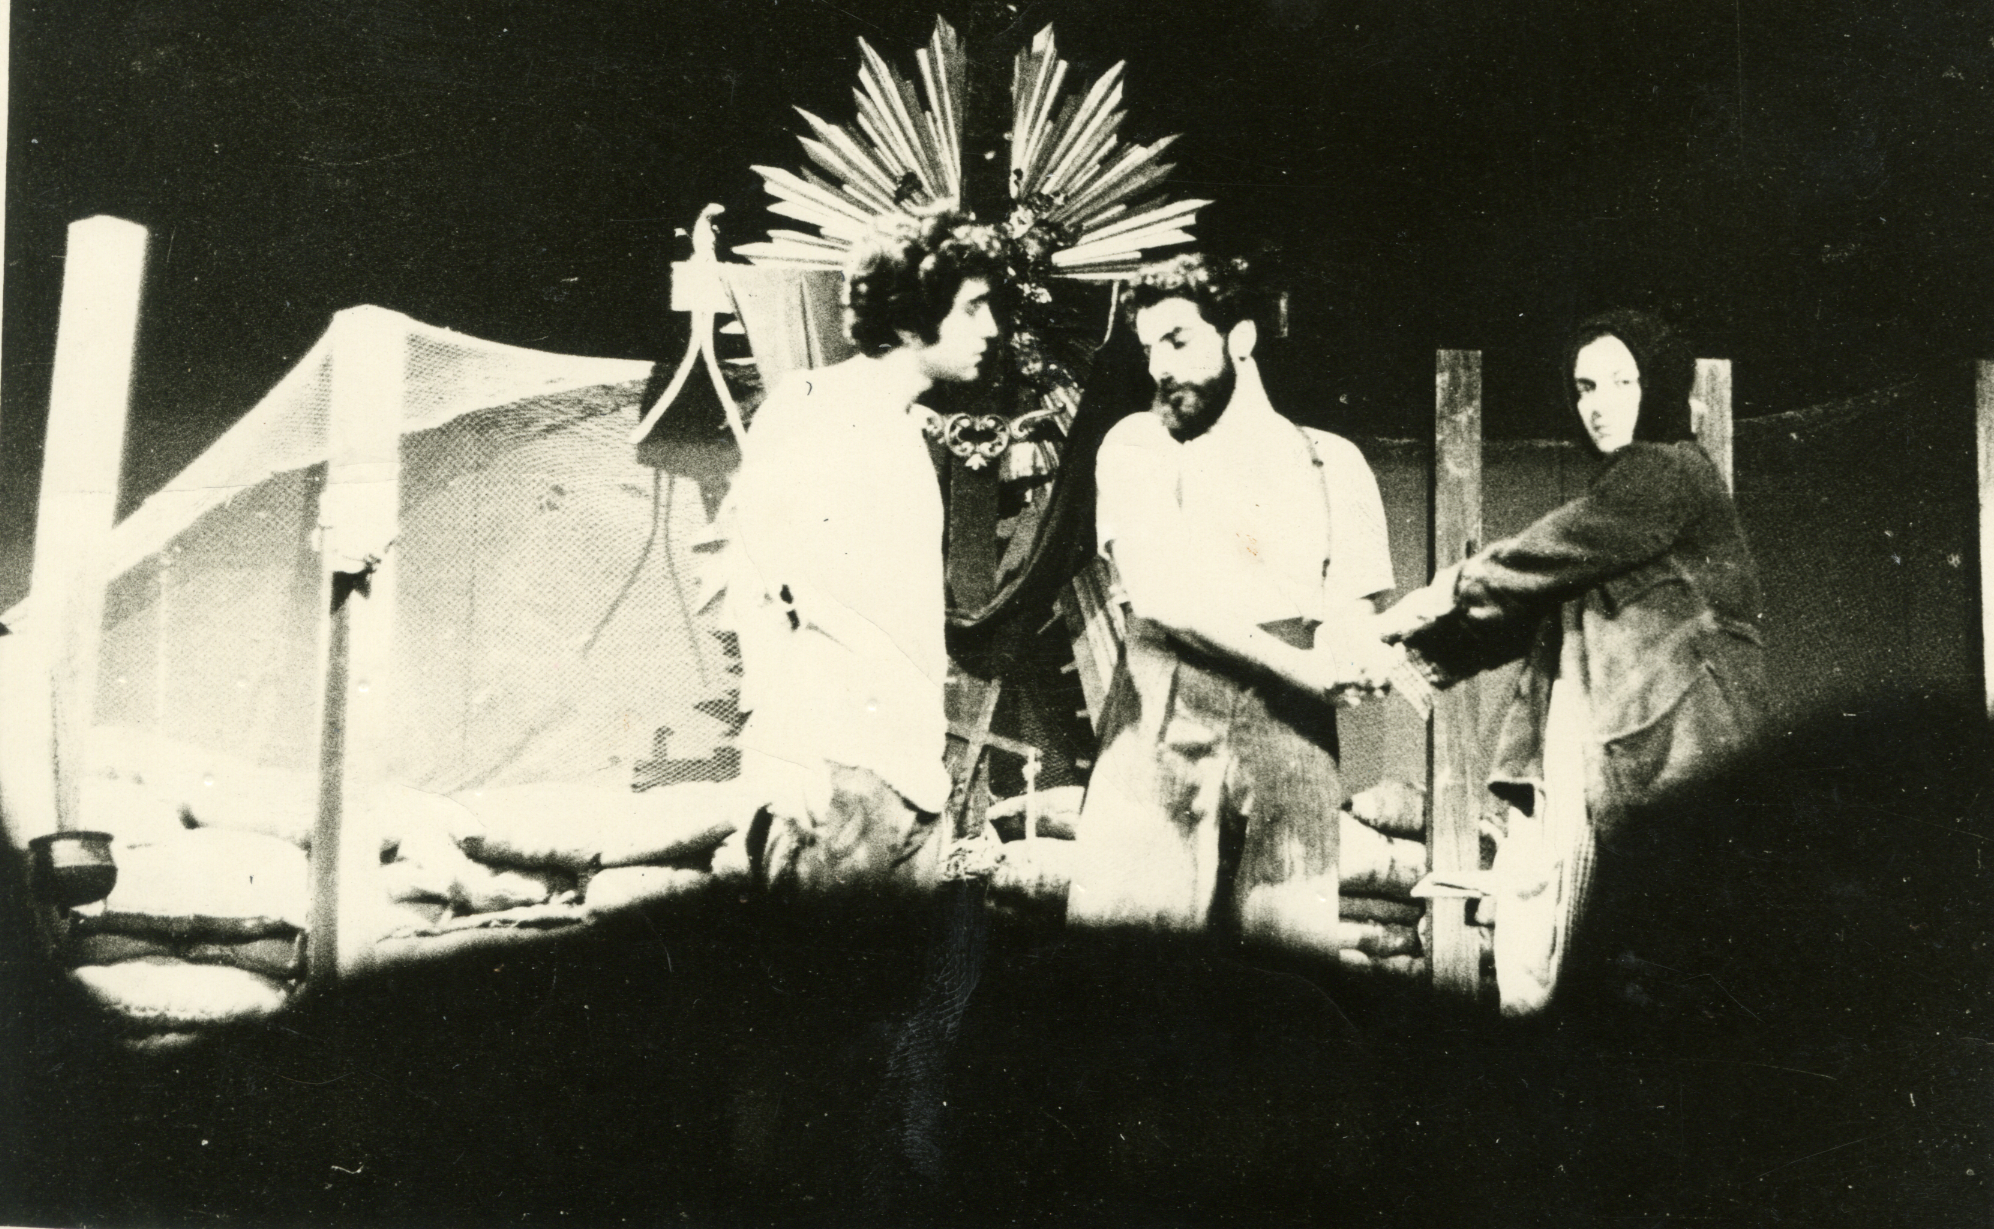
\includegraphics[width=\columnwidth]{./media/IMAGEM39.png}
\caption{André Gouveia como José, Sérgio Mindlin como o operário Pedro Jáqueras e Bety Chachamovitz como Senhora Carrar. 1968. Autor desconhecido. Acervo
Diários Associados. Arquivo Público do Estado de São Paulo.}
\end{figure}

\begin{itemize}
\item
  Irmão e combatente
\end{itemize}

A chegada do irmão de Tereza da frente de batalha aumenta a pressão
sobre ela. O operário Pedro Jáqueras é um lutador da resistência. Ele
veio visitá-la para recuperar os fuzis que foram guardados pelo cunhado.
Precisa levá-los para os combatentes, o momento da guerra é crítico. Ele
sabe que Tereza, depois da morte do marido, procurou refúgio na igreja e
que não vai facilitar a entrega das armas. Ao mesmo tempo, reconhece a
simpatia do sobrinho pela resistência quando o rapaz se põe a seu lado:

OPERÁRIO - Os fuzis são o que mais fazem falta no momento. Aqui no
povoado vocês não têm fuzis?

MÃE \textit{cortando a conversa} - Não!

JOSÉ - Algumas pessoas esconderam os que tinham: enterraram no chão como
se fossem batatas.

Tereza evita seguir no assunto da guerra. A atriz, na montagem do TUSP,
segura o irmão pelas mãos e encara o público. Há carinho entre eles, mas
a atenção dele está no sobrinho, que aproxima seu corpo como alguém
disponível. Em seguida haverá um jogo de cartas entre ambos, que se
transforma em oportunidade de aprendizado sobre a luta:

OPERÁRIO - Trapaceando sempre?

JOSÉ \textit{rindo} - Eu já trapaceei alguma vez?

OPERÁRIO - Me parecia. Então eu vou cortar todas as vezes: assim, vale
tudo. Na guerra todos os truques são válidos, é ou não é?

\textit{A Mãe olha com desconfiança.}

JOSÉ - Esse é o pior dos trunfos.

OPERÁRIO - Ainda bem que você diz isso... Ah, e sai logo de ás! Você
blefou, mas não foi um pouquinho caro? Desfez a sua artilharia pesada, e
agora eu entro com minhas bombinhas. (\textit{Recolhe a vaza}.) Venha a
nós! Audácia é uma coisa muito boa, meu filho, e audácia você tem, mas
não é prevenido.

\begin{figure}
\includegraphics[width=\columnwidth]{./media/IMAGEM40.png}
\caption{André
Gouveia como José Carrar. 1968. Fotógrafo: Victor Knoll. Acervo pessoal}
\end{figure}

\begin{figure}
\includegraphics[width=\columnwidth]{./media/IMAGEM41.png}
\caption{À esquerda, ator não identificado. À direita, Renata Souza Dantas como
Manuela. 1968. Fotógrafo: L. Pinto. Acervo Última Hora. Arquivo Público
do Estado de São Paulo.}
\end{figure}

\begin{figure}
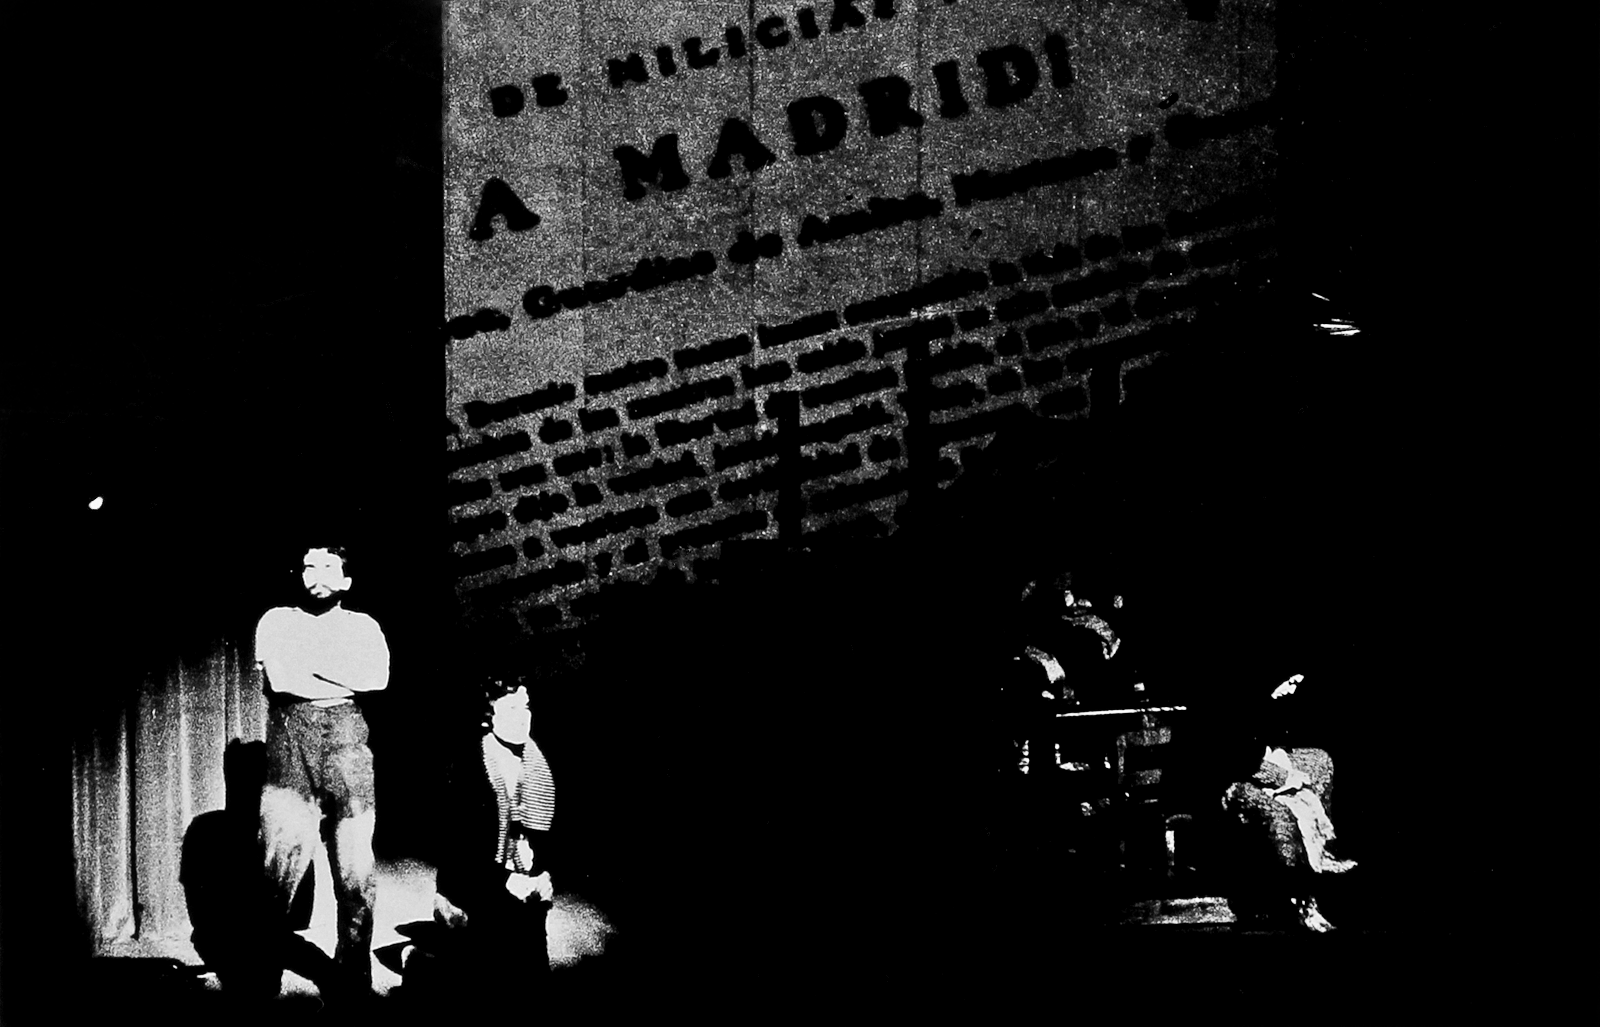
\includegraphics[width=\columnwidth]{./media/IMAGEM42.png}
\caption{Sérgio Mindlin como o operário Pedro Jáqueras, ator não identificado e
Bety Chachamovitz como Senhora Carrar. 1968. Fotógrafo: Victor Knoll.
Acervo Flávio Império.}
\end{figure}

\begin{itemize}
\item
  Passagem épica
\end{itemize}

A ação da peça acontece na Andaluzia, região de histórico revolucionário
anarquista, mas que desde o golpe de estado dos generais em julho de
1936 tinha a presença de forças nacionalistas. Ainda assim, cidades
importantes como Málaga, onde o irmão de Tereza combate pelos
republicanos, só vieram a cair no ano de 1937, quando Brecht escreveu o
texto. A casa dos Carrar está próxima a uma zona de conflito, o que é
indicado pelo constante som de bombardeios. O aposento dramático vibra
pelos ruídos da guerra.

O maior dos momentos “épicos” produzido pela sonoridade é o desfile das
brigadas internacionais antifascistas. Após a chegada do irmão, Tereza
recebe também a visita de Pablo, um ferido com a cabeça enfaixada e o
braço na tipóia. Ela cuida do rapaz e com sua saída se escutam os sons
dos motores dos caminhões que indicam a passagem dos combatentes,
transportados para a frente de batalha em Motril. Trechos do cancioneiro
revolucionário são cantados em línguas diversas, como se viessem dos
carros de transporte, o que indica as nacionalidades dos brigadistas
explicitadas pelos comentários do irmão operário. A montagem do TUSP,
além das canções indicadas por Brecht, como \textit{Bandiera Rossa,}
destaca a \textit{Marcha de las Brigadas Internacionales}. O espetáculo faz
uso nesse momento da projeção novamente: exibe fotos de jornais de época
que noticiam a campanha dos resistentes. Ocorre aí um momento gestual
não previsto pelo texto, talvez no trecho que convoca à defesa dos
filhos por meio da luta:

\begin{quote}
Camaradas, cubrid los parapetos,

que la vida no es vida sin la paz.

Defended con el pecho vuestros hijos,

os ayuda la solidaridad;
\end{quote}

José, o filho mais novo, empunha por um instante o fuzil do tio, para
saudar os combatentes que passam lá fora. O gesto de “pegar em armas” se
dá na relação com a imagem audiovisual. O espetáculo amplia a
interrupção épica da ação dramática. O comentário gestual antecede o
retorno à ficção, com a entrada em cena de Manuela.

\begin{figure}
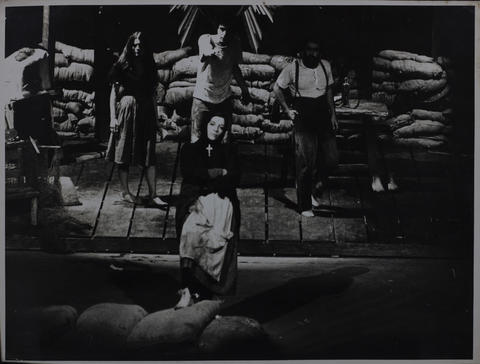
\includegraphics[width=\columnwidth]{./media/IMAGEM43.jpg}
\caption{Renata Souza Dantas como Manuela, André Gouveia como José, Sérgio
Mindlin como o operário Pedro Jáqueras e Bety Chachamovitz como Senhora
Carrar. 1968. FUNARTE/ Centro de Documentação e Pesquisa.}
\end{figure}

\begin{figure}
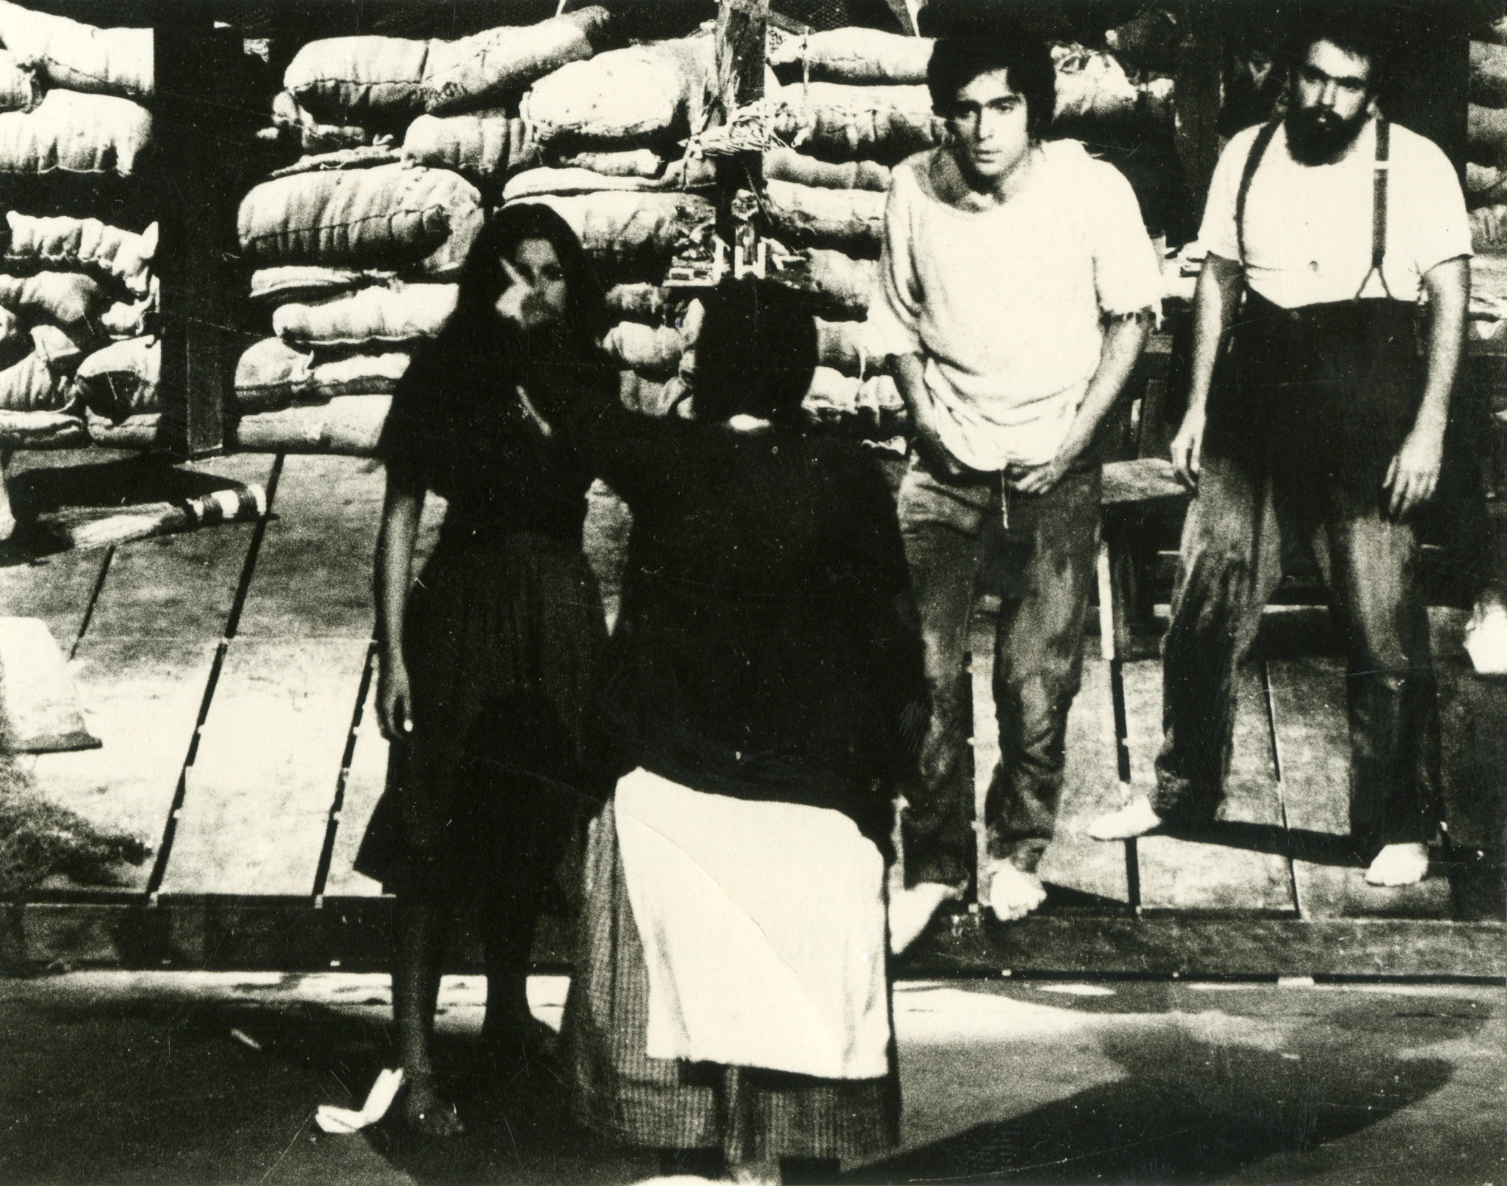
\includegraphics[width=\columnwidth]{./media/IMAGEM44.png}
\caption{Renata Souza Dantas como Manuela, André Gouveia como José, Sérgio
Mindlin como o operário Pedro Jáqueras e (de costas) Bety Chachamovitz
como Senhora Carrar. 1968. Fotógrafo: Victor Knoll. Acervo Flávio Império.}
\end{figure}

% \textit{ou}

% Autor desconhecido. Acervo Diários Associados. Arquivo Público do Estado
% de São Paulo.

\begin{figure}
\includegraphics[width=\columnwidth]{./media/IMAGEM45.png}
\caption{Renata Souza Dantas como Manuela. 1968. Fotógrafo: Victor Knoll. Acervo
pessoal.}
\end{figure}


\begin{figure}
\includegraphics[width=\columnwidth]{./media/IMAGEM46.png}
\caption{Renata Souza Dantas como Manuela, André Gouveia como José, Sérgio
Mindlin como o operário Pedro Jáqueras e Bety Chachamovitz como Senhora
Carrar. 1968. Fotógrafo: Victor Knoll. Acervo Flávio Império}
\end{figure}

% \textit{ou} Autor desconhecido. Acervo Diários Associados. Arquivo Público
% do Estado de São Paulo.

\begin{itemize}
\item Acusação de Manuela
\end{itemize}

Ainda se escutam ao longe as brigadas quando Manuela, namorada de Juan,
aparece na casa dos Carrar: está revoltada com a omissão da família.
Nesse dia havia se acertado que todos os homens da comunidade em
condições de combater se juntariam às barricadas e Juan não compareceu.
Descobre-se neste momento a razão pela qual a mãe mandou o jovem pescar:
para que ele não soubesse do movimento coletivo.

O debate é direto. Manuela sobe o tom contra Tereza, chegando a acusá-la
de apoiar os generais franquistas. A Senhora Carrar, por sua vez, se
apega às tarefas do cotidiano: cuida do pão no forno, argumenta que a
pesca é o ofício da família. Quando o confronto chega ao ápice, há uma
estilização das marcações da cena do TUSP: Manuela, José e Pedro se põem
lado a lado, alinhados no confronto a Tereza. Ela se vira ao público.
Está irredutível. À frente dela, a plateia também recebe a acusação.
Mesmo os comentários moralistas e pessoais de Manuela, quando diz que
deixará Juan por sua covardia, não encontram resposta de Tereza.

\begin{figure}
\includegraphics[width=\columnwidth]{./media/IMAGEM47.png}
\caption{Moacyr Urbano Villela como o Padre, Sérgio Mindlin como o operário Pedro Jáqueras e Bety Chachamovitz como Senhora Carrar. 1968. Fotógrafo:
Victor Knoll. Acervo Flávio Império.}
\end{figure}


\begin{figure}
\includegraphics[width=\columnwidth]{./media/IMAGEM48.png}
\caption{Sérgio Mindlin como o operário Pedro Jáqueras, Moacyr Urbano Villela
como o Padre e Rose Lacreta como Senhora Carrar. 1968. Autor
desconhecido. Acervo Última Hora. Arquivo Público do Estado de São
Paulo.}
\end{figure}

\begin{itemize}
\item
  Defesa do padre
\end{itemize}

A aparição do Padre dá corpo a um tema anunciado pela grande cruz. Logo
após sua entrada e a oferta de vinho por Tereza, escutam-se nos
auto-falantes as palavras do General Queipo de Llano. Elas provêm do
rádio do vizinhos da família Carrar, os Perez. Eles sobem o volume do
instrumento para que Tereza escute, para que ela não se aliene dos
horrores do tempo. Toda a vizinhança apoia a resistência, e a emissão
sonora, já ocorrida na primeira cena de Brecht, vem agora como como
acusação à neutralidade do sacerdote. A voz do general reproduz mentiras
fascistas sobre o assassinato de padres pelos comunistas, e critica a
posição de parte da igreja internacional. Tereza apresenta o sacerdote a
seu irmão como alguém que a ajudou quando seu marido morreu, alguém que
acolhe os órfãos dos pais combatentes. O Padre apoia a decisão de
Tereza. O Operário o questiona sobre sua posição política:

OPERÁRIO - E o senhor também é neutro?

PADRE - Que quer dizer?

OPERÁRIO - É isto mesmo: partidário da não-intervenção. E sendo pela
não-intervenção, admite, no fundo, todo esse banho de sangue em que os
senhores generais vêm mergulhando o povo espanhol.

PADRE \textit{(levando as mãos à altura da cabeça, num gesto defensivo)} -
Isso eu não admito!

OPERÁRIO (\textit{fitando-o com os olhos semicerrados)} - Fique um instante
assim com as mãos para o alto: nessa mesma posição, cinco mil dos nossos
homens tiveram de sair de casa, durante o cerco de Badajoz, e nessa
mesma posição foram abatidos a tiros.

No espetáculo do TUSP, o irmão conversa com o Padre apoiado em Tereza: o
Operário põe as duas mãos sobre o ombro da irmã, como quem tenta
acordá-la ou apenas se conectar a ela. Ele tenta fazê-la entender, pelo
gesto, que a abstenção não implica proteção, pois queira ou não ela é
uma parte daquele povoado, não da igreja, numa luta promovida pelo
capital. No momento de maior confronto entre os dois, o Operário
questiona diretamente a plateia, e o Padre responde de costas para ele:

OPERÁRIO - A senhora Carrar e os filhos não levantam um dedo contra o
General Franco. Sendo assim, a senhora Carrar e os filhos estão em
segurança?

PADRE - A julgar com a humanidade ...

OPERÁRIO - A julgar com a humanidade, como?

PADRE - Que garantia o senhor quer que eu lhe dê?

OPERÁRIO - Nenhuma. Eu quero apenas a sua opinião: a senhora Carrar e os
filhos dela estão em segurança?

\textit{O Padre silencia.}

OPERÁRIO - Acho que já respondeu. O senhor é honesto.

\begin{figure}
\includegraphics[width=\columnwidth]{./media/IMAGEM49.png}
\caption{Sérgio Mindlin como o operário Pedro Jáqueras, Cida Previatti como
Senhora Perez, André Gouveia como José e (à frente) Bety Chachamovitz
como Senhora Carrar. 1968. Fotógrafo: Victor Knoll. Acervo Flávio
Império.}
\end{figure}

\begin{itemize}
\item
  Julgamento da Senhora Perez
\end{itemize}

Enquanto Tereza acompanha a saída do Padre, seu irmão procura os fuzis.
Está decidido a levá-los. Tereza volta antes que ele possa sair. Tira as
armas das mãos do irmão e passa a vigiá-las. Pedro ameaça chamar o
sobrinho pescador Juan para partir com ele. Chega, então, a Senhora
Perez, a vizinha da casa que liga o rádio para provocar a família
Carrar. Ela acaba de perder uma filha no \textit{front}, é capaz de
compreender a dor de Tereza. Dirige-se a ela sem agressividade. Tenta se
desculpar pelas importunações à família.

De novo, o espetáculo dirige a argumentação às costas da Mãe Carrar,
agora sentada num plano mais baixo, no proscênio. Na imagem, a senhora
Perez está sentada no centro do palco. Ladeada pelo tio e filho de
Tereza, sua posição é a de uma testemunha ou mesmo uma juíza portadora
da voz do povoado. Apela à consciência mais íntima e ao mesmo tempo
social da vizinha, a da pobreza: “Andam dizendo por aí que a senhora é
do outro lado, mas eu desminto isso sempre. Nós sabemos muito bem qual é
a diferença que existe entre ricos e pobres.”

Tereza está inabalável na decisão de que seus filhos não serão soldados
porque “não são gado para matadouro”, mas se vê obrigada a uma defesa
sem sentido do bom senso dos generais. Haveria nos generais fascistas
uma capacidade qualquer de escuta, dada por sua humanidade, pois eles
não são “nenhum terremoto com quem não se pode argumentar.” Acuada, ela
contra-ataca a vizinha de modo pessoal e desonesto, não aceita ser
julgada:

MÃE - {[}...{]} E a Senhora Perez, por que é que fica aí sentada em
minha sala a me dizer uma porção de coisas? Está pensando que eu não sei
de tudo o que vem me dizer? Se a sua filha está morta, agora é a vez dos
meus: não é isso o que a senhora quer? A senhora invade a minha casa,
como se fosse um cobrador de impostos: mas eu já paguei a minha cota.

Na imagem fotográfica, a posição de Tereza é tranquila, resolvida. Seus
olhos, porém, procuram os do público e se voltam várias vezes aos fuzis,
dispostos no chão, à sua frente.

\begin{figure}
\includegraphics[width=\columnwidth]{./media/IMAGEM50.png}
\caption{André Gouveia como José e Bety Chachamovitz como Senhora Carrar. 1968.
Fotógrafo: Victor Knoll. Acervo pessoal.}
\end{figure}

\begin{figure}
\includegraphics[width=\columnwidth]{./media/IMAGEM51.png}
\caption{Bety Chachamovitz como Senhora Carrar e André Gouveia como José. 1968.
Fotógrafo: Victor Knoll. Acervo Flávio Império.}
\end{figure}

\begin{itemize}
\item
  Luta pelas armas
\end{itemize}

A partida da Senhora Perez reacende o conflito. O irmão está furioso com
a impassividade de Tereza diante dos apelos. O filho José decide partir
com o tio, à revelia da mãe.

No texto de Brecht, ela se senta sobre a caixa de armas. Quando José faz
menção de sair, ela corre até ele e o abraça fortemente, momento em que
o filho grita ao tio para que pegue as armas. A reação de Tereza no
original é divertida: ela finge ter se machucado na corrida, e começa a
mancar, vitimizando-se, num teatrinho que lhe permita retomar o controle
das armas, o que dura até o momento em que tem o pressentimento que algo
muito ruim e triste aconteceu lá fora.

Na montagem do TUSP, de modo diverso, ocorre um confronto físico com seu
filho mais novo pela posse das armas. Quando o rapaz tenta pegá-las,
esgueirando-se no chão, a mãe se põe sobre ele, de pé. Por baixo das
pernas de Tereza, o deslocamento do filho sugere um parto, numa
estilização intencional. Em seguida, o rapaz mexe no nariz em sinal de
desprezo ostensivo pela mãe, e se afasta com uma das armas para o fundo
do palco. Ela o segue, e se ajoelha diante do filho, que ergue o fuzil
muito perto da grande cruz. É neste ponto que Tereza percebe que o barco
de Juan não está mais visível no mar, desapareceu do horizonte. Sua
explicação inicial e descabida é que Juan fugiu para se engajar na luta,
que as importunações e visitas durante o dia acobertaram sua partida.
Seu discurso é duro, enunciado como uma praga:

MÃE - Se Juan se alistou na milícia, que seja maldito. Que veja que Deus
não permite que zombem dele. E que um pobre não pode lutar contra os
generais. {[}...{]} E se ele me aparecer de volta {[}...{]} digo a ele
que não quero em minha casa ninguém manchado de sangue. Eu o arrancarei
de meu coração como se arranca um pé gangrenado! {[}...{]} Talvez vocês
aprendam isso antes que os generais tenham acabado conosco: aquele que
usar de violência morrerá pela violência.

\begin{figure}
\includegraphics[width=\columnwidth]{./media/IMAGEM52.png}
\caption{Atrizes não identificadas. 1969. \textit{Frame} do documentário
\textit{Festival Mondial du Théâtre de Nancy} (1999).}
\end{figure}

\begin{itemize}
\item
  Coro de Senhoras Carrar
\end{itemize}

Na peça de Brecht, a última frase em fúria de Carrar - “quem com ferro
fere, com ferro será ferido” - é interrompida por um burburinho de vozes
de três mulheres que rezam uma Ave-Maria. Elas precedem a entrada de
dois pescadores que trazem o corpo de Juan Carrar, morto pelos
fascistas, e uma vela manchada de sangue. O drama trágico se consuma na
evidência maior, a morte.

Na montagem do TUSP, a raiva da Mãe gera um movimento formal inesperado,
que surge da plateia. É a surpresa maior do espetáculo: um coro de dez
mulheres, até então oculto, surge por trás do público. Seu figurino
estilizado se diferencia dos trajes realistas das demais personagens.
Elas se movem ritmicamente, usam meias-máscaras e túnicas pretas com
apliques dourados, portam incensos e manipulam barulhentas matracas de
semana santa, que produzem um som de metralhadoras. Deslocam-se
hieráticas, mas seus ruídos sugerem os tiros que mataram Juan.

Seu aparecimento é anunciado com grandiloquência, ao som de \textit{Carmina
Burana}, de Carl Off, compositor estimado por Goebbels e pelos nazistas.
Na atmosfera litúrgica do ambiente agora incensado, elas se aproximam do
palco, se viram para o público e recitam em coro trechos da maldição de
Tereza sobre Juan, assumindo-se como ecos da Mãe. O debate do espetáculo
ganha forma nova: não há neutralidade possível. Há ruído, fúria, e o
anúncio da morte.

\begin{figure}
\includegraphics[width=\columnwidth]{./media/IMAGEM53.png}
\caption{Atores não identificados. 1969. \textit{Frame} do documentário
\textit{Festival Mondial du Théâtre de Nancy} (1999).}
\end{figure}

\begin{itemize}
\item
  \textit{Mater Dolorosa}
\end{itemize}

Tereza se multiplica, assim, nas mulheres do coro. Sua fala dura, porém,
não corresponde a seu sentimento real. A entrada em cena do corpo de seu
filho Juan tudo muda: a dor da mãe agora é imensa, ela desaba, sem que
nada antes tenha anunciado esse colapso. Sua dor é a de todas as
mulheres do coro. O TUSP fez uso, nessa coreografia do colapso, de uma
musicalidade religiosa, da polifonia gregoriana. O quadro cênico se
converte em seguida na imagem de uma \textit{Mater Dolorosa} coletiva. Uma
das atrizes se destaca do coro e assume a cena da \textit{Pietà}: o corpo
do filho é deitado sobre as pernas dela, que ampara o cadáver. Há algo
de \textit{kitsch} na religiosidade assim exposta, que combina com a cruz
em cacarecos. Em algumas apresentações, a camisa de Juan contém o mesmo
desenho do sangue na camisa de Edson Luís. Em outras, baixou-se a
bandeira com a referência ao assassinato, para que fosse usada como
mortalha. A ambiguidade irônica se amplia com a entrada da música \textit{A
whiter shade of pale}, sucesso \textit{pop} de Procol Harum. A imagem expõe
agora seu lado de redenção mistificadora, de consumo religioso, de
santificação mercantil do próprio guerrilheiro.

\begin{figure}
\includegraphics[width=\columnwidth]{./media/IMAGEM54.png}
\caption{Bety Chachamovitz como Senhora Carrar. 1968. Fotógrafo: Victor Knoll.
Acervo Flávio Império.}
\end{figure}

\begin{itemize}
\item
  Decisão das Terezas
\end{itemize}

O texto de Brecht cria pressões trágicas sobre o drama de Tereza Carrar.
Seu filho foi assassinado gratuitamente. Os franquistas atiraram assim
que avistaram o barco de Juan. A mãe compreende de imediato:

MÃE \textit{com simplicidade} - A culpa foi do boné.

PESCADOR 1 - Como assim?

MÃE - Todo puído: um homem decente não usa um boné assim.

PESCADOR 1 - Então eles podem ir atirando em qualquer um que esteja com
o boné puído?

MÃE- Eles podem, sim. Eles não são homens. Eles são uma lepra e é
preciso queimá-los com um ferro em brasa como se queima uma lepra.

\textit{Os fuzis da Senhora Carrar} é uma peça estruturalmente dramática,
com breves aberturas épicas. Entretanto, a hesitação da Mãe Carrar entre
a neutralidade e a resistência não se liga a seu caráter ou consciência:
o que se mostra em cena é a pressão da realidade social e política, uma
recusa idealista feita em nome da preservação da vida, que é destruída
com a presença da morte. A trajetória de Tereza é a da impossibilidade
de uma decisão autônoma. Sua tragicidade resulta da condição de mulher
pobre, pescadora e mãe. É uma pessoa que supõe, por algum tempo, que a
humanidade deveria ser a transformabilidade razoável de todas as
relações, sobretudo em contextos em que tudo tende ao inumano.

Quando a montagem do TUSP foi apresentada, alguns grupos de mães de
jovens militantes que atuavam politicamente se organizavam para garantir
que as manifestações estudantis fossem realizadas de forma pacífica. Em
um momento de limite de paciência no trato com a violência de estado,
uma dessas mulheres teria dito “esta mão de mãe que espalha as lágrimas
também pega em fuzil”.\footnote{Quem narra o acontecimento é Daniel
  Aarão Reis Filho em \textit{68: a paixão de uma utopia}, livro que
  combina fotografias de Pedro de Moraes aos textos de Reis Filho (Rio
  de Janeiro: Editora Fundação Getulio Vargas, 1998, p. 152).}

É nesse contexto que a multiplicação de mães Carrar em meio à plateia
ganha um sentido de metáfora da participação. Quando Tereza decide pela
luta, é o coro que o faz. O coletivo é quem pega os fuzis espalhados
pela plateia, sob os assentos dos espectadores. Seu gesto coral de
mostrar as armas, em seguida, é um exemplo, uma incitação a que o
público participe na luta contra a ditadura. A tragicidade ganha
expressão formal na coreografia que se encaminha da ficção para a vida.

\begin{figure}
\includegraphics[width=\columnwidth]{./media/IMAGEM55.png}
\caption{Moacyr Urbano Villela como Bispo acompanhado de ator não identificado.
1968. Fotógrafo: Victor Knoll. Acervo pessoal.}
\end{figure}

\begin{itemize}
\item
  Guerra capitalista
\end{itemize}

Quando Brecht escreveu sua dramaturgia, em 1937, a Guerra Civil
Espanhola estava ainda em curso. A Espanha estava dividida pelos
combates, os republicanos ainda controlavam regiões estratégicas como
Madrid, Valência e a Catalunha. Durante toda a peça, se escutam os
bombardeios na frente de batalha, que se intensificam na cena final,
indicando que os franquistas romperam o bloqueio. É para esse combate
derradeiro que as personagens partem apressadas. Quando o TUSP encenou
seu espetáculo, a ditadura franquista, com sua história de genocídio,
seguia no poder, como um dos últimos regimes fascistas da Europa. Era um
assunto da atualidade brasileira.

A cena final do espetáculo do TUSP foi organizada como uma procissão
trágica. Com as armas empunhadas, o coro acompanha a saída da Mãe
Carrar. O corpo do filho é deixado no palco, como um Cristo abandonado.

A montagem não parece ter ilusões sobre as dificuldades da passagem da
decisão ao ato político, ao ressaltar seu caráter mortuário. O TUSP cria
um epílogo que não existe no texto de Brecht: enquanto o coro deixa a
sala, o proscênio é ocupado por uma figura eclesiástica. O Padre da peça
é paramentado como um bispo grotesco, veste um manto de borracha preta,
coloca no rosto uma máscara contra gases e, sobre sua cabeça, uma mitra
dourada. O \textit{napalm} mencionado no início parece ressurgir no
figurino. Com as mãos banhadas de sangue, o bispo animalizado oficia uma
missa mortuária. O gesto teatral se baseia numa fala do Operário que
alude ao mais famoso de Pilatos: “as pessoas que não querem assumir
nenhuma culpa acabam lavando as mãos em bacias de sangue. E esse sangue,
depois bem que se vê nas mãos!”

A figura episcopal não surge, porém, sozinha. Vem ao proscênio
acompanhada por um homúnculo cabeçudo, alegoria do militarismo, uma
criatura do capitalismo bélico. Ele se junta ao bispo para tripudiar
sobre qualquer visão da humanidade fundada na igualdade. Seu discurso
faz uso de frases do monarquista Calvo Sotelo e de Franco, entre outras,
para explicitar a relação entre fascismo, capitalismo e religião: “Pelas
brechas abertas por nossos canhões penetrarão o Evangelho e o lucro!”. A
fala inclui comentários sarcásticos sobre a importância da virgindade
das moças. Na montagem do espetáculo no Festival de Nancy, o TUSP
procurou conectar o texto à situação local. Na locução gravada, ouvia-se
o discurso traduzido em francês, com um sotaque que se assemelhava a De
Gaulle. Ele enfrentava naqueles dias um revés eleitoral que levou à sua
renúncia. Não se tratava de acusar De Gaulle de fascista, mas de apontar
semelhanças na opção pelo capital contra os comunistas e socialistas. A
alusão ao líder francês incendiou a plateia francesa, que depois da peça
se reuniu para cantar a \textit{Internacional}.

Após o discurso fascista, os alto-falantes voltam a enunciar a descrição
monótona dos efeitos do \textit{napalm}. O espetáculo do TUSP se encerra
com essa celebração grotesca da guerra capitalista, que diz respeito à
Espanha, ao Vietnã e ao Brasil. A plateia não sabe como se comportar, se
deve aplaudir ou não.

\chapter{MOBILIZAÇÃO CULTURAL ALÉM DO ESPETÁCULO: A REVISTA \textit{APARTE}}

\begin{figure}
\includegraphics[width=\columnwidth]{./media/IMAGEM56.png}
\caption{Renata Souza Dantas e André Gouveia com camisetas que anunciavam o
espetáculo \textit{Os fuzis} no Rio de Janeiro. julho de 1968. Autor
desconhecido. Acervo Última Hora. Arquivo Público do Estado de São
Paulo.}
\end{figure}

Não é incomum que um grupo de teatro complemente sua atuação cênica com
publicações em que possa divulgar as sínteses de seus estudos e suas
pesquisas artísticas. Essa tradição de longa duração na literatura
ocidental se expandiu no período do modernismo, do início do século XX,
quando a arte de vanguarda se pensava como uma elaboração
artístico-crítica, ligada a \textit{manifestos} de tipos variados, o que
exigia uma rede de articulações teóricas. A revista se oferecia, assim,
como um lugar de trabalho comum, um ponto de aglutinação entre dimensões
locais e internacionais.

No momento de maior expansão do teatro de \textit{agitprop}, por exemplo,
nos primeiros anos da União Soviética, o coletivo Blusa Azul teve um
veículo impresso ligado a atividades formativas, como a escola de
preparação de agitadores. A publicação ajudou a multiplicar a
experiência do coletivo pelo país, e contribuiu para a formação de quase
cinco mil brigadas pela Europa.

Na Alemanha, país que teve grande influência do grupo soviético, os
coletivos de \textit{agitprop} também mantiveram revistas. A
\textit{Arbeiterbühne und Film} {[}\textit{Teatro e Cinema dos
Trabalhadores}{]} era destinada ao debate teórico. E o grupo Megafone
Vermelho manteve uma publicação própria, com difusão de repertório para
as encenações.\footnote{Sobre os grupos de \textit{agitprop} na União
  Soviética e na Alemanha, veja-se “A Arma do Teatro” de Eugenia Casini
  Ropa, em seu \textit{A Dança e o Agitprop} (São Paulo: Perspectiva, 2014,
  p. 111-158).}

No Brasil foram muitos os casos semelhantes. O Teatro de Arena de São
Paulo, por exemplo, depois do golpe de 1964, publicou as formulações
teóricas de Augusto Boal em torno do chamado \textit{Sistema Coringa.} E o
mesmo foi feito mais tarde, com as técnicas do \textit{Teatro Jornal} e com
as \textit{Categorias de Teatro Popular}.\footnote{Alguns desses materiais
  foram traduzidos e publicados em revistas teatrais internacionais no
  período, como a cubana \textit{Conjunto} e a francesa \textit{Travail
  Théâtral}, e deram origem a livros futuros.}

Anos antes, o processo de formação do CPC teve avaliação teórica no
ensaio famoso de Vianinha \textit{Do Arena ao CPC}, publicado na revista
\textit{Movimento} da UNE, reflexão que antecedeu a criação de um setor de
publicações do coletivo, em que o carro chefe seriam os \textit{Cadernos do
Povo Brasileiro}, que tratavam de assuntos culturais e sociais variados.
O contemporâneo Movimento de Cultura Popular, de Pernambuco, produziu
\textit{Livros de Alfabetização} e boletins mensais sobre teatro.

Ainda mais cedo, temos notícia do jornal \textit{Quilombo}, editado pelo
Teatro Experimental do Negro a partir de 1948, das \textit{Edições TEP}, do
Teatro do Estudante de Pernambuco, que reuniam a produção de seus
integrantes, e da \textit{Revista do Teatro Amador}, seguida pela
\textit{Revista de Estudos Teatrais}, ambas do Federação Paulista de
Amadores Teatrais na década de 1950.

Os primeiros trabalhos do TUSP em torno do I Congresso Nacional de
Teatro Universitário e dos cursos e leituras dramáticas trouxeram, de
pronto, a necessidade de um registro e de uma maior difusão dos estudos
realizados.

A Comissão de Dramaturgia se empenhava na tradução de textos e de
documentos inéditos. Gerava materiais para uma atividade maior de
sentido literário, que poderia ir além do trabalho teatral em curso. O
TUSP passou a publicar apostilas, a fazer cópias de suas traduções, a
mimeografar transcrições de peças antigas. Esses textos corriam de mão
em mão, em circulação restrita. São documentos hoje praticamente
desaparecidos. Uma peça então pouco lida da cena teatral brasileira,
\textit{O homem e o cavalo}, de Oswald de Andrade, tornou-se conhecida no
meio universitário paulistano por ações como essas.

Antes mesmo da organização de um setor de publicações, o TUSP
experimentava parcerias com jornalistas amigos, colaboradores da grande
imprensa da época, como forma de publicização e convocação dos
estudantes.

O jornalismo, num momento em que isso era possível, foi muito utilizado
para a difusão do projeto do grupo, como se vê numa matéria não assinada
em \textit{O Globo} que tem ares de um manifesto, composta a partir de uma
uma fala enunciada por um integrantes do grupo:

\begin{quote}
“No caso de \textit{A Exceção}, escolhemos primeiro o público - na época,
achamos necessário atingir os operários -, e depois o tipo de mensagem.
A luta de classes, analisada do ponto de vista científico numa estrutura
social, rompendo com a estrutura, ou seja, tornando-se uma sociedade sem
classe, precisava ser abordada. Encontramos em Brecht, didático e
aberto, um diálogo compreensível para o operário, havia elementos de
teatro revista, musicado por Rogério Duprat e Damiano Cozzella.

Quando os estudantes começaram a se manifestar, escolhemos \textit{Os
fuzis}, de acordo com suas ideias ativas e imediatas: eles sabem que não
vão mudar a sociedade, isso é tarefa do operário, mas sabem que são o
estopim. Procuramos uma mensagem, considerando o universo como é,
quietista e neutro. A própria neutralidade é falsa: ao nos omitirmos,
concordamos com o status, a tomada de posição é necessária. Importante
definir qual o tipo de participação e escolhemos Brecht pela discussão
de neutralidade em dois níveis e a indefinição do texto. Esta peça é
muito particular, foi escrita por encomenda, solicita da plateia uma
cumplicidade. Trata da Guerra Civil Espanhola e do envolvimento de
franceses e alemães.

Diferimos da linha de Marcuse, porque ela apresenta uma solução a longo
prazo, nós pretendemos resolver antes, através do estudante, que voltará
às suas classes depois de cumprir o seu papel. Ninguém trai sua origem.
Poucos permanecerão na luta. O teatro, para nós, é uma discussão em
torno de alguns problemas considerados importantes e tem uma função
política acentuada.”\footnote{“Gente nova em teatro novo”, \textit{O
  Globo}, Rio de Janeiro, 10 jul. 1968, p. 4.}
\end{quote}

A decisão de editar uma revista própria tem muitas razões, sendo a mais
evidente delas a vontade de encontrar um lugar de debates que não está
dado na grande imprensa e que também não se encaixa no mundo acadêmico,
com sua exigência de cientificidade e referenciamento que muitas vezes é
refratária ao debate livre e ao ensaísmo.

O interesse pela “função política acentuada” estava, também, na origem
da \textit{aParte}, essa revista de curta duração que foi um dos grandes
trabalhos do TUSP. Seu objetivo era apresentar alguns dos mais
importantes debates da época sobre a relação entre estética e política,
interligando as áreas do teatro, cinema, literatura e artes visuais. Sua
perspectiva editorial era criteriosa e as excelentes traduções,
realizadas pelos próprios integrantes do grupo.

\textit{aParte} foi impressa pela editora \textit{Teoria e Prática}, do
arquiteto Sérgio Ferro, que também era responsável por uma revista de
esquerda com o mesmo nome. A Comissão de Publicação da \textit{aParte}
tinha autonomia em relação à editora e ao próprio grupo teatral. A
diretora responsável era Betty Milan e o programador visual, Ricardo
Ohtake.

Planejada para ser bimestral, ela teve colaborações regulares de pessoas
que acompanhavam os ensaios teatrais do TUSP de perto. Embora não
estivessem em cena nos espetáculos, eram interlocutores da Comissão de
Dramaturgia. É o caso de Albertina Costa, Oswaldo C. Louzada Filho e
Jean-Claude Bernardet, presentes também no Congresso e nos cursos do
grupo, Cláudio Torres Vouga, companheiro de Albertina, Walnice Nogueira
Galvão, que trabalhou na adaptação do texto da montagem de \textit{Os
fuzis} com Flávio Império, e da própria Betty Milan.

Além desse núcleo, que se dedicou em especial às reflexões e à crítica
de cinema, a Comissão de Publicação realizou entrevistas, convidou
intelectuais a escreverem artigos sobre temas de interesse do grupo,
traduziu entrevistas, roteiros e textos de intervenção. A revista teve
apenas três números, todos de 1968, sendo que o terceiro foi apreendido
na gráfica antes que qualquer exemplar pudesse ser recuperado.

Quando observamos os dois notáveis números remanescentes, é possível
intuir que o primeiro, lançado em seguida à estreia de \textit{Os fuzis},
busca sistematizar e aprofundar os estudos de formação do grupo e do
espetáculo, enquanto o segundo documenta as primeiras realizações
artísticas e demarca o posicionamento estético do próprio TUSP em
relação ao teatro paulistano, com debates que seriam aprofundados nos
números seguintes.

\begin{figure}
\includegraphics[width=\columnwidth]{./media/IMAGEM57.pdf}
\caption{\textit{aParte} número 1, como se vê na capa, tem como questão orientadora
a luta antiimperialista. A guerrilha é discutida como forma praticada na
Guerra do Vietnã, como técnica do teatro de intervenção.}
\end{figure}

A revista abre com uma entrevista de Luiz Valdez, ex-integrante da San
Francisco Mime Troupe que fundou \textit{El Teatro Campesino}, o primeiro
grupo de teatro latino dos Estados Unidos. Ele discute a criação do
grupo, em 1965, e seu objetivo de agitação dos trabalhadores imigrantes
latinos que organizaram uma grande greve no sul da Califórnia. Valdez
narra como foram estabelecidas as relações com os sindicatos aos quais o
grupo se vinculou, e os expedientes de que adotaram para criar suas
intervenções, conhecidas como \textit{Actos}. Descreve uma experiência de
trânsito entre a produção artística, o meio estudantil, e o mundo dos
trabalhadores com o qual Valdez tinha contato por ser filho de
imigrantes.

No mesmo número, outra tradução procura sugerir caminhos para o teatro
engajado universitário. As \textit{Dez teses sobre o teatro universitário},
do dramaturgo alemão Martin Wiebel, interessaram ao TUSP por sua recusa
ao esteticismo autorreferente da cena universitária, como se lê na nota
introdutória da revista ao texto:

\begin{quote}
consideramos muito oportunas as críticas do autor ao pseudo-vanguardismo
e à procura do efeito fácil enquanto formas de fuga da realidade, que,
às vezes sob aspectos diferentes, têm prejudicado também o nosso TU
{[}teatro universitário{]}.\footnote{\textit{aParte}, São Paulo, n. 1,
  mar.-abr. 1968, p. 27.}
\end{quote}

Não é certo que haja aí uma crítica às proposta de grupos universitários
como o Tese ou o Tuca, mas o fato é que a tradução visava lembrar a cena
artística estudantil de que seu compromisso crítico e político deveria
dar forma a uma qualidade estética igualmente radical, em torno de uma
experimentação socialmente consequente, conforme propõe Wiebel em sua
última tese:

\begin{quote}
\textit{Tese X} - A independência que caracteriza o teatro universitário
nos oferece a possibilidade da experiência, no sentido estrito da
palavra, isto é, a realização de um projeto anterior. Dois caminhos se
abrem aqui:

a) a experiência estilístico-artesanal com os meios teatrais, buscando a
mais alta perfeição.

b) o comprometimento no nível da crítica social com suas possibilidades
de trabalho em equipe.\footnote{Idem, p. 28.}
\end{quote}

Este debate sobre vanguardismo e possibilidade de uma intervenção
política no teatro assume outra dimensão quando o grupo convida como
interlocutores os principais diretores do teatro profissional de São
Paulo (e talvez do Brasil) àquele tempo, Augusto Boal e Zé Celso, para
entrevistas polêmicas. Publicadas juntas, como um díptico, numa seção
intitulada \textit{Depoimentos sobre o teatro brasileiro hoje}, as
entrevistas são da maior importância pela reflexão que trazem sobre a
mudança dos tempos da cena politizada brasileira.

Augusto Boal, na esteira da autocrítica da esquerda ao possível
populismo do teatro político do pré-64, resguarda a força do teatro
político de agitação e propaganda tal como feito nos centros populares
de cultura e comenta a violência gerada pelo golpe contra aquelas
experiências. Zé Celso, por sua vez, critica a tradição da cena
politizada no estilo do Teatro de Arena, com seu suposto propósito de
“imitação do povo”, e defende um modelo mais agressivo de atuação, que
tenha a cultura e a moralidade da plateia pequeno-burguesa como alvo.
Ele formula, assim, a ideia de um teatro da crueldade brasileiro. Ambos
recorrem à imagem da guerrilha para defender suas posições. Para Zé
Celso, interessa a dimensão de ruptura da guerrilha:

\begin{quote}
A eficácia do teatro político hoje é {[}...{]} uma guerra contra a
cultura oficial, a cultura de consumo fácil. Pois com o consumo não só
se vende o produto, mas também se compra a consciência do consumidor. O
sentido da eficácia do teatro hoje é o sentido da guerrilha teatral. Da
anticultura, do rompimento com todas grandes linhas do pensamento
humanista.\footnote{“Depoimentos sobre o teatro brasileiro hoje: Augusto
  Boal e José Celso Martinez Corrêa”. \textit{aParte}, São Paulo, n. 1,
  mar.-abr. 1968, p. 20-21.}
\end{quote}

Para Boal, sua agilidade, a capacidade de se expandir e multiplicar na
relação com uma população oprimida:

\begin{quote}
Dezenas de CPCs respondiam quase que imediatamente às variações da
política nacional e internacional. Nunca o teatro foi tão contemporâneo
dos acontecimentos representados. {[}...{]} Eu estou certo de que nunca,
em nenhuma parte do mundo, o teatro foi tão guerrilheiro. Nesse tempo,
companhias profissionais se deslocavam pelo Brasil, especialmente pelo
Nordeste, levando espetáculos nas ruas, circos, igrejas. E quando a peça
escolhida exigia condições especiais, atores se reuniam e montavam, eles
próprios, o texto.\footnote{Idem, p. 17}
\end{quote}

Zé Celso e Boal, o Oficina e o Arena, eram as grandes referências do
TUSP para seu trabalho. Havia, porém, críticas dos estudantes a suas
posições. O confronto do pensamento de ambos visava abrir espaços para
que uma outra via surgisse.

A pesquisa de caminhos novos era, de qualquer modo, uma necessidade do
momento. O próprio Augusto Boal vinha refletindo sobre os rumos da arte
de esquerda. E tentava realizações práticas baseadas nessa avaliação
crítica. Um exemplo teatral disso, de simbolismos contraditórios, é a
peça \textit{A lua muito pequena e a caminhada perigosa}, também publicada
na revista \textit{aParte}, e que integraria depois o espetáculo
\textit{Primeira Feira Paulista de Opinião}.\footnote{O livro organizado
  pelo LITS, \textit{Primeira Feira Paulista de Opinião} reúne pela
  primeira vez o conjunto das dramaturgias que integrava o espetáculo em
  uma edição crítica. Nela, são comparadas as diversas versões de cada
  texto. No caso de \textit{A lua muito pequena}, são comparadas as versões
  de três roteiros do espetáculo com o texto publicado em vida pelo
  autor e o texto publicado na \textit{aParte} (São Paulo: Expressão
  Popular, 2016, p. 177-197).} O texto é um relato lírico-coral sobre os
últimos momentos de Che Guevara na Bolívia, até sua captura e
assassinato pelo exército dos Estados Unidos. Publicado ao lado de
fotografias de Che, a peça encerra o conjunto de referências à guerrilha
que aparecem na revista.

A \textit{aParte 1} tem ainda um ensaio visual sobre a Guerra do Vietnã,
cujas imagens ressurgem em cena no prólogo do espetáculo \textit{Os fuzis},
e o relato de uma impressionante experiência de cinema produzida pelos
guerrilheiros vietnamitas. Trechos do roteiro de um filme produzido pela
Frente de Libertação Nacional do Vietnã do Sul, \textit{Phin Phong Su},
colocam lado a lado a descrição da força bélica, os ruídos de bombas, as
rajadas de metralhadoras, as armadilhas, e imagens de união da
população, crianças dançando e jovens estudando, ao som de músicas
alegres. Na apresentação dessa atividade guerrilheira de propaganda, o
texto afirma:

\begin{quote}
Glauber Rocha disse que fazer cinema é ter uma ideia na cabeça e uma
câmera na mão. Qualquer guerrilheiro-cineasta vietcong avançou muito
além disso: uma ideologia na cabeça, um fuzil na mão direita, uma câmera
na mão esquerda.\footnote{“Um fuzil na mão direita, uma câmera na mão
  esquerda”. \textit{aParte}, São Paulo, n. 1, mar.-abr. 1968, p. 50.}
\end{quote}

Como contraponto à sequência vietnamita, são reproduzidos trechos de
outro filme de propaganda, \textit{Enquanto homens corajosos morrem}, do
conservador americano Fulton Lewis III, que defende a atuação dos
Estados Unidos na Guerra do Vietnã. A obra combina imagens do conflito a
discursos abstratos sobre a posição do país, em defesa da “paz e da
liberdade”, com \textit{flashes} de manifestações contra a guerra em que há
acusações aos militantes pacifistas por seus supostos vínculos com o
comunismo e falta de patriotismo. Em seguida a esse roteiro patético, um
anúncio do espetáculo \textit{Os fuzis} questiona em caixa-alta:

\textit{Mas que espécie de gente somos nós?}

Flávio Império, diretor do espetáculo, também assina um texto nesse
número inicial da \textit{aParte}. Ele comenta o filme \textit{O Evangelho
segundo São Mateus}, de Pasolini, de quem também é traduzida uma
entrevista. O cineasta italiano comenta seu processo criativo, o
trabalho de composição minuciosa dos planos, de montagem, e a
preferência por colaborar com não-atores, aspectos que rondam a
experiência de \textit{Os fuzis}.

Completam o volume outros textos sobre cinema: a crítica de Jean-Claude
Bernardet a \textit{Todas as mulheres do mundo}, exibido em pré-estreia
pelo TUSP, e a resenha de seu livro \textit{Brasil em tempo de cinema},
feita por Betty Milan.

O livro polêmico de Bernardet, àquele tempo na contramão da esquerda
convencional, contribuiria para o crescimento da onda crítica que reduz
toda arte politizada da época a uma atitude supostamente paternalista na
relação com o povo. O núcleo do argumento de Bernardet é que em alguns
filmes do Cinema Novo a classe média tenta produzir cultura para o povo,
mas se distancia da realidade de sua própria classe. Por isso, o Cinema
Novo acaba por gerar um cinema teoricamente feito para classes
populares, mas incapaz formalmente de chegar até elas, e que perde a
chance de um diálogo mais real com a classe média que frequenta as salas
de cinema.

Milan reconstrói o ponto de vista do livro, elogia a disposição crítica
do autor, mas não deixa de apontar suas fragilidades: faltaria à obra
uma especificação desse ente abstrato chamado “classe média”, além a
vontade real de entender se não há caminho possível para o cinema além
da “classe média”. Suas palavras parecem expressar a visão do TUSP sobre
a questão:

\begin{quote}
E o público que mais interessava aos cineastas, o dos sindicalistas por
ex.? No horizonte da única perspectiva apontada pelo A., não se situa o
cinema que elabore propostas revolucionárias e atue nos setores
revolucionários mais consequentes.\footnote{“Brasil em tempo de cinema”.
  \textit{aParte}, São Paulo, n. 1, mar.-abr. 1968, p 81.}
\end{quote}

Na última seção da revista do TUSP, intitulada Infra Vermelho,
Jean-Claude Bernardet é um dos colaboradores. É composta de pequenos
artigos críticos sobre filmes e espetáculos do Brasil e do mundo. Entre
os vários textos está uma dura crítica de Flávio Império a duas
montagens dirigidas por Adhemar Guerra, \textit{Marat-Sade} e \textit{Oh!, que
delícia de guerra,} exemplos de subserviência cultural a centros
estrangeiro e de normalização dos conflitos. Na visão de ambas, segundo
o crítico-cenógrafo, “a guerra é folclórica, os loucos são figuras de
cera”.

\includegraphics[width=\columnwidth]{./media/IMAGEM58.jpg}

O segundo número da revista \textit{aParte} abre com um manifesto, uma
\textit{Proposta sobre a crítica e a produção artística}. Numa refutação
aberta às entrevistas de Zé Celso e de Augusto Boal divulgadas no número
anterior, os artistas do TUSP esboçam uma poética de ordem negativa: não
querem ser o antropófago José Celso, que ao fim das contas será
“devorado pela sociedade de consumo que tanto quis devorar”; e nem
Augusto Boal, homem de outro teatro que procura uma eficácia política,
mas que recaiu no estilo “de pé!, povo!” mostrado nas montagens
Zumbi-Tiradentes, e assim se converteu num “papa da festividade e
renovador do teatro catártico”.

A opção deliberada por “pichar unilateralmente os dois melhores, mais
brilhantes, e mais responsáveis profissionais do nosso teatro” era uma
incitação a que o teatro universitário do tempo percebesse a
insuficiência política de projetos de arte que, em tempo de fechamento
social, pareciam condenados ao naufrágio.

Sem certeza sobre a própria linha estética-política, o TUSP se inspirava
num caminho “apenas indicado” por uma citação de Régis Debray, extraída
de seu livro sobre a guerrilha, \textit{Revolução na Revolução}: “O
intelectual deve se suicidar como categoria social, para renascer como
revolucionário.”\footnote{“Proposta sobre a crítica e a produção
  artística”. \textit{aParte}, São Paulo, n. 2, mai.-jun. 1968, p. 4.}

A autocrítica da condição de intelectual não implicava, porém, uma
recusa à aprendizagem. Mas ela deveria vir como práxis, pois fosse o que
fosse, o grupo deveria procurar uma atitude de “alunos da Revolução”.

O brevíssimo texto que vem em seguida ao manifesto trata de \textit{Os
fuzis de Dona Tereza Carrar}. Ali os artistas reafirmam sua busca de uma
nova forma para o teatro universitário, que combine gestos de sentimento
e reflexão, no que parecem querer conjugar aspectos dos projetos
poéticos do Arena e do Oficina:

\begin{quote}
Ninguém chega à consciência política por via meramente racional; a
emoção se esgota no instante. Os dois se completam. Dos intestinos à
cabeça, é esse o caminho da consciência para a pequena burguesia de
barriga cheia.\footnote{“Os fuzis de Dona Tereza Carrar”. \textit{aParte},
  São Paulo, n.2, mai.-jun. 1968, p. 5.}
\end{quote}

Complementa essa espécie de segundo “editorial” da revista um ensaio
visual com imagens de Victor Knoll do espetáculo \textit{Os fuzis,} ao lado
de uma única imagem de \textit{A exceção e a regra}.

A obra de Peter Weiss, autor de Marat-Sade, segue discutida pelo grupo
com a publicação de seu artigo \textit{10 hipóteses de um autor neste mundo
dividido}, em que ele avalia as dificuldades e a importância de
“escolher um lado” no planeta cindido pela Guerra Fria, pois se há
dogmatismo no bloco oriental, existe também o esforço positivo de
equiparações. Como artista oriundo de um mundo burguês, ele constata que

\begin{quote}
a arte sem amarras atinge a arrogância, já que naqueles países em que as
diferenças raciais e oposições de classe são mantidas pela força, as
prisões estão repletas de torturados que lutam pela mudança.\footnote{“10
  hipóteses de um autor neste mundo dividido”. \textit{aParte}, São Paulo,
  n. 2, mai.-jun. 1968, p. 15.}
\end{quote}

Alguns dos debates da \textit{aParte} 1 reaparecem no segundo número. O
Cinema Novo volta a ser discutido em sua realidade produtiva. E o tema
da dialética possível entre arte de vanguarda e intervenção social, das
entrevistas de Zé Celso e Boal, é reposto no estudo de Walnice Nogueira
Galvão, \textit{A Moderna Música Popular Brasileira: uma análise
ideológica}. Ela ali ecoa também parte das posições de Bernadet, ao
sugerir que a denúncia das mazelas brasileiras posta ao lado de imagens
da beleza da vida no morro, da simplicidade no sertão, cria uma
mistificação, uma zona de conforto ideológico, que atrai o público
intelectualizado mas o exime da necessidade de agir politicamente. Seu
ensaio recorre a canções de autores como Caetano Veloso, Chico Buarque,
Edu Lobo, Geraldo Vandré e Gilberto Gil. A autora finaliza sua análise
com critérios ativistas:

\begin{quote}
Em circunstâncias muito mais difíceis foi lançado o \textit{Carcará}, que
está aí, solitário, para pôr em xeque a afirmação de que não há nenhuma
canção brasileira que proponha a ação. Não há nenhuma, de fato. Exceto
\textit{Carcará}. Que foi um sucesso extraordinário de público, donde
também não se pode alegar prudência comercial. A única dúvida cabível é
achar insuficiente como proposta o refrão: “Pega, mata e
come.”\footnote{“MMPB: uma análise ideológica”. \textit{aParte}, São Paulo,
  n.2, mai.-jun. 1968, p. 31.}
\end{quote}

Ainda no campo da música, Oswaldo C. Louzada Filho escreve \textit{O
Contexto Tropical}, em que analisa a forma de representação do
imaginário brasileiro expressa no disco \textit{Tropicália}, com particular
atenção à canção título, de Caetano Veloso:

\begin{quote}
Na verdade, toda a música se realiza numa alternância de festa e
proposta de luta, degradação e louvação, brasileirismo lírico e miséria.
{[}...{]} As imagens, referências e situações que compõem a Tropicália
acabam configurando um \textit{kitsch} particular.\footnote{\textit{aParte},
  São Paulo, n.2, mai.-jun. 1968, p. 69.}.
\end{quote}

Seu argumento parece preparar a observação célebre de Roberto Schwarz no
ensaio \textit{Cultura e Política} sobre a imagem tropicalista em sua
capacidade de “encerrar o passado na forma de males ativos ou
ressucitáveis”, sugerindo que “são nosso destino, razão pela qual não
cansamos de olhá-la.”\footnote{“Cultura e Política, 1964-1969", de
  Roberto Schwarz, publicado em \textit{O pai de família e outros estudos}
  (São Paulo: Companhia das Letras, 2008, p. 92).} Em ambos os casos, a
análise - verdadeira no que se refere à opção por uma alegoria
estabilizadora -, parece desconsiderar os aspectos musicais
mobilizadores e inventivos, sem os quais essa obra não teria a força que
tem.

A perspectiva guerrilheira - o grande assunto do TUSP naquele momento -
reaparece no comentário crítico de Sérgio Muniz aos filmes \textit{Le 17ème
Paralele}, de Joris Ivens, e \textit{Loin du Vietnam}, de Chris Marker, no
que é complementada pelo debate em torno das guerras de libertação das
antigas colônias portuguesas, em especial Guiné Bissau, na carta de
Valentino Orsini, traduzida com o título \textit{Hipótese ideológica aberta
pela explosão da bomba H}. O documento registra um momento de origem, em
que a crítica ao “eurocentrismo” ainda não era feita em termos puramente
culturais.

A revista conta com um caderno especial dedicado ao debate sobre uma das
grandes armas ideológicas da ditadura, a censura. Destacado em páginas
pardas no centro da publicação, o dossiê analisa o problema geral,
reproduz um discurso do chefe do Departamento Federal de Segurança
Pública em homenagem à censura, expõe os critérios dos censores naquele
momento da ditadura, faz uma lista de filmes censurados, e ainda torna
pública a opinião do governo sobre o perigo da influência comunista,
questão materializada em análises reacionárias de obras como o filme
\textit{Os fuzis} feitas por funcionários ligados ao Ministério da Justiça
e dos Negócios Interiores.

O procedimento de compilação desses materiais lembra os recursos de
teatro documentário utilizados em \textit{Os fuzis de Dona Tereza Carrar}.
Os textos são expostos de modo a que um entre em atrito com o outro, a
que se contradigam. No final do caderno, uma nota anuncia o projeto do
TUSP de mapear os atos de censura e divulgar denúncias encaminhadas à
revista.

Por fim, o tema da comunicação de massa é discutido por Gabriel Cohn em
\textit{McLuhan e o ecumenismo controlado}, um artigo em que discute um
livro que se tornou referência para a época, \textit{Understanding Media}.
Crítico em relação à ênfase formal e técnica de McLuhan quando descreve
o poder dos \textit{media}, o autor percebe aí um movimento de
deslocamento: ao invés de debater o controle produtivo dos meios de
comunicação, Mcluhan prefere discutir a força dos meios e das
programações no controle das pessoas, com uma postura quase fatalista
quanto à possível controlabilidade dos sistemas midiáticos. Cohn
contrapõe a essa visão uma perspectiva mais histórica, como a de Walter
Benjamin em seu \textit{A obra de arte na era de sua reprodutibilidade
técnica}:

\begin{quote}
Ao pôr ênfase no caráter histórico dos modos de percepção, é possível a
um autor como W. Benjamin ir muito além de McLuhan apesar de partir de
proposições mais modestas, e mostrar como a crise da própria produção e
recepção da obra artística na época da produção em massa tem raízes
sociais que implicam em alterar a própria função da arte, num sentido
que torna suscetível de ser suporte de uma ação política, de expansão da
consciência social.\footnote{“McLuhan e o ecumenismo controlado”.
  \textit{aParte}, São Paulo, n. 2, mai.-jun. 1968, p. 55.}
\end{quote}

O debate é complementado pelo ensaio de Betty Milan, que vem a seguir,
sobre o filme \textit{Privilégio}. A obra trata do poder capitalista dos
veículos de comunicação, com base na história de um astro da música
\textit{pop} que se torna uma marionete dos setores conservadores do Reino
Unido quando sua imagem e popularidade são convertidas em instrumento do
fundamentalismo religioso e do nacionalismo fascista. O TUSP ilustra o
ensaio com \textit{frames} de uma celebração religiosa mostrada no filme, e
com a reprodução de uma carta do arcebispo de São Paulo - Agnelo Cardeal
Rossi - ao Vaticano solicitando a admissão de Roberto Carlos ao
beija-mão do Papa Paulo VI. No documento, usado como ilustração, o
arcebispo metropolitano argumenta que sua “amizade com este jovem,
expoente da música popular chamada Iê-iê-iê, tem sido benéfica para a
mocidade em geral”.\footnote{\textit{aParte}, São Paulo, n. 2, mai.-jun.
  1968, p. 61.}

O interesse pela indústria cultural segue uma análise de Ângela Mendes
de Almeida intitulada \textit{Mistificação e Realidade}, sobre a revista
\textit{Realidade}. A publicação, de alto nível para a imprensa da época,
tinha começado a circular em abril de 1966. Em seu número especial de
setembro de 1967, ela se dispôs a traçar um “retrato da juventude
brasileira de hoje”, baseado em entrevistas de múltipla escolha. A
autora descreve as várias falhas sociológicas da pesquisa, que não expõe
seus métodos e que caracteriza seus entrevistados segundo classificações
a-históricas como “o jovem universitário”, “o jovem bancário”, “o jovem
camponês”, “o jovem interiorano”, sem qualquer menção a aspectos de
classe, gênero, raça. Mesmo considerando que “\textit{Realidade} não é, nem
de longe, uma revista retrógrada” por tratar de “teses avançadas” como
“divórcio e liberdade sexual”, o que está em jogo para a autora é uma
visão ideológica confortadora sobre o mundo estabelecido, e a proposição
dessa visão como “modelo educativo”:

\begin{quote}
O modelo proposto enquadra as inovações nos limites da inocuidade e
omite o que possa lançar problemas na cabeça da juventude. Os frutos
desse investimento, a Abril os colherá a médio e a longo prazo. Serão os
frutos da passividade política e da subjugação do indivíduo à ideologia
difundida pelos meios de comunicação de massa.\footnote{“Mistificação e
  realidade”. \textit{aParte}, São Paulo, n. 2, mai.-jun. 1968, p. 67.}
\end{quote}

Apesar da variedade de assuntos, a segunda edição de \textit{aParte}
encontra unidade na crítica à facilitação artística, na procura da
atitude guerrilheira e revolucionária, na continuidade do desejo de
aproximar mundos populares e de pesquisa crítica avançada. O maior
símbolo disso é a escolha de traduzir o roteiro completo de um grande
filme como \textit{Subversivos}, dos irmãos Taviani, que ocupa uma boa
parte da revista. Em contraste com uma obra fílmica admirada, a
publicação - que foi a última que chegou aos leitores - se encerrava com
a seção Infra Vermelho, feita de comentários breves ao cinema feito na
época por artistas como Buñuel, Arthur Penn, Alain Resnais e o
brasileiro Leon Hirszman.

\includegraphics[width=\columnwidth]{./media/IMAGEM59.jpg}


\includegraphics[width=\columnwidth]{./media/IMAGEM60.pdf}

Antes mesmo da decretação do Ato Institucional número 5, em dezembro de
1968, a revista \textit{aParte} foi perseguida pela polícia da ditadura
devido à suspeita, sugerida por seu nome, de ser um veículo da
organização Ação Popular (AP). A associação era equivocada. Os
integrantes do TUSP que estavam engajados na atividade política
pertenciam a outras organizações. Em agosto de 1968 foi expedido um
mandado de busca e apreensão que resultou no recolhimento de todos os
exemplares do terceiro número da revista, referente ao bimestre
julho-agosto, ainda na gráfica.

Do terceiro número destruído sobrou apenas o registro da capa: o rosto
de Che Guevara numa releitura \textit{pop} de Claudio Tozzi da famosa
fotografia de Alberto Korda ilustrava a publicação. Três textos eram
anunciados: \textit{Arte e revolução em Havana}, \textit{França de maio} e a
peça de Guarnieri, \textit{Animália}, apresentada naquele ano no espetáculo
\textit{Primeira Feira Paulista de Opinião}, da qual a peça de Boal sobre
Che também fazia parte.

A \textit{aParte} foi uma revista tão incomum e inspirada quanto as obras
teatrais do grupo. Seu compromisso era com o aprendizado livre, com a
crítica alegre, com a procura de movimentos independentes. O número não
divulgado talvez contivesse estudos sobre a nova arte teatral,
cinematográfica e musical que se fazia na América Latina, inspirada pela
revolução de Cuba, nos anos anteriores ao fechamento de ciclo promovido
pelos Estados Unidos com os muitos golpes militares patrocinados pelo
continente.

\chapter{IMPROVISAÇÕES DO TEATRO ÉPICO NO BRASIL}

\textit{Os fuzis de Dona Tereza Carrar} foi a maior realização da breve
história do TUSP. Estreou em 3 de maio de 1968 no Teatro Ruth Escobar,
em São Paulo. Foi apresentada ainda no Teatro Maria Della Costa, no TUCA
e no Teatro Oficina. Fora da capital, foi exibida no Teatro de Alumínio,
em Santo André, então ocupado pelo grupo Teatro da Cidade, de Heleny
Guariba. Circulou pelo interior e foi mostrada em Santos e Curitiba. Fez
uma breve temporada de grande repercussão no Rio de Janeiro, entre o
Teatro Nacional de Comédia e o Teatro Miguel Lemos.

Em 1969, o espetáculo foi convidado ao Festival Mundial de Teatro
Universitário de Nancy, na França. Era o mais politizado e influente dos
festivais europeus no que se refere à cena jovem mundial.
Apresentaram-se ali nomes centrais da vanguarda teatral como Peter
Brook, Pina Bausch, Jerzy Grotowski, Tadeusz Kantor, ao lado de
coletivos anticapitalistas como El Teatro Campesino e o Teatro
Experimental de Cali, da Colômbia. Havia ainda grupos de vanguarda de
países como Zaire e Japão. O Teatro de Arena, o Oficina e o grupo do
TUCA mostraram seus trabalhos no festival.

A versão de Brecht encenada pelo TUSP foi saudada com entusiasmo pelo
público e pela crítica em Nancy, num momento de debates sobre o teatro
épico e o teatro popular, quando a cena experimental francesa refletia
sobre a renovação do teatro politizado tendo como base a experiência de
grupos como o Théâtre du Soleil. Havia um certo esgotamento da
representação social convencional, e havia aqueles que propunham uma
dramaturgia íntima que fosse capaz de mostrar os estragos subjetivos do
capitalismo.

Pela qualidade do espetáculo mostrado e pela sintonia com as questões da
época, o TUSP foi convidado a se reapresentar no encerramento do
festival - num ano em que já não havia mais premiação para o melhor
espetáculo. Na volta a São Paulo, realizou uma última e breve temporada
de \textit{Os fuzis} no Theatro São Pedro como contrapartida ao patrocínio
público recebido para financiar parte da viagem.\footnote{Há uma grande
  dose de contradição, mas a concorrência entre o patrocínio público por
  alguns órgãos e perseguição por outros durante a ditadura é mais comum
  do que se imagina.}

Naquele ano de 1969, depois de Nancy, aproximava-se o fim de um ciclo de
trabalhos notáveis. O momento político era dos mais difíceis. O Ato
Institucional número 5 instaurou uma onda de violências maiores do
aparelho repressivo. Boa parte do elenco estava na mira da perseguição
política. Diante disso, alguns atores permaneceram na Europa, escolhendo
o exílio, e não participaram das apresentações no Theatro São Pedro.

Era recente a lembrança do violento ataque do Comando de Caça aos
Comunistas ao \textit{Roda viva} no Teatro Ruth Escobar. E por terem
participado das vigílias de proteção ao teatro atacado, corriam o risco
de estarem sendo monitorados. A repercussão de \textit{Os fuzis}, por sua
vez, atraiu a atenção policial sobre o grupo. Os rumores do teor
revolucionário da encenação tinham chegado aos ouvidos da repressão após
o sucesso da temporada carioca. Em 1968, Carlos Swan, denunciou, na
coluna social do jornal \textit{O Globo,} o caráter revolucionário da
montagem. Ele afirma: “o texto brechtiano é pretexto para um comício
político, em que distúrbios recentemente ocorridos na Guanabara são
inseridos no contexto da guerra civil espanhola”.\footnote{“Uma salada”,
  \textit{O Globo}, Rio de Janeiro, 9 jul. 1968, p. 4.} A nota ensejou uma
manifestação da censura federal, que começava a operar naquele ano. A
censora se viu obrigada a observar que a montagem do TUSP foi liberada
anteriormente pela Seção de Censura regional de São Paulo. Num texto com
ares de crítica jornalística, a funcionária destaca as qualidades do
conjunto do elenco e da direção, mencionando o aplauso “sem restrições”
dos críticos profissionais. E procura afastar as acusações mais graves
ao dizer que

\begin{quote}
não aparecia o cadáver do estudante Nelson Luiz {[}sic{]} nem sua camisa
manchada de sangue cobria o cadáver de um personagem, nem tampouco,
foram ouvidos comentários pelo microfone, fora de cena, sobre os
incidentes de março de 1968.\footnote{“Informação” por Marina de Mello
  Ferreira. Rio de Janeiro, 10 de julho de 1968. Processo de censura da
  peça \textit{Os fuzis da Senhora Carrar}, de Bertolt Brecht. BR DFANBSB
  NS.CPR.TEA, PTE.370.}
\end{quote}

Menos reacionária do que o colunista, ela comenta a leviandade do
comentário de Swan, ao citar outro episódio, quando ele elogiou um
espetáculo de dança sequer realizado. Contudo, sobre \textit{Os fuzis},
registra a possibilidade de ser um trabalho de fato instrumentalizado
por organizações de luta armada, e afirma:

\begin{quote}
Constituindo a encenação um desafio às estruturas sociais, políticas e
religiosas, poderiam ser investigadas as verdadeiras causas de tal
atitude, partindo de um grupo de jovens estudantes. Urge saber quem os
lidera e qual a extensão dos focos de insurreição.\footnote{Idem.}
\end{quote}

Parte da atenção também se devia a uma associação com dois outros
espetáculos de grande repercussão naquele ano de 1968: a \textit{Primeira
Feira Paulista de Opinião}, do Teatro de Arena, sobre a obra de seis
dramaturgos convidados, que estreou como ato de desobediência civil à
censura; e \textit{Roda viva}, montagem de Zé Celso a partir da peça de
Chico Buarque. Ambas estiveram em cartaz ao mesmo tempo no Teatro Ruth
Escobar e encarnaram, nos dizeres do crítico João Apolinário, os dois
caminhos teatrais que correspondiam ao “momento histórico”: “Parece
evidente que teatro popular significa teatro de agressão ou teatro
didático.”\footnote{A crítica foi reproduzida na edição crítica da
  \textit{Primeira Feira Paulista de Opinião} (São Paulo: Expressão
  Popular, 2016, p. 351).}

A qualidade estética do TUSP, na procura de um caminho próprio em
relação às influências do Teatro de Arena e do Oficina, era o que
conferia à sua posição política uma intensidade vibrante. Não há dúvida
que a contribuição de Flávio Império neste processo de mediações com os
modelos foi decisiva. Oriundo do Teatro de Arena, ele era cenógrafo de
\textit{Roda viva}, como já observado neste livro, enquanto dirigia \textit{Os
fuzis}. Utilizou procedimentos de visualidade semelhantes nos dois
espetáculos: uma grande cruz no cenário, como indicação alegórica do
conluio entre fascismo, religião e capitalismo. As encenações ainda
tinham em comum a presença do coro que ocupa a plateia e desloca a
narrativa. O de \textit{Roda viva}, porém, descia do palco numa provocação
acusatória aos espectadores, enquanto o coro das mães de \textit{Os fuzis},
formava-se na plateia e no mesmo plano convocava o público a se unir aos
artistas numa luta fora do teatro. O sentido épico da cena do TUSP
procurava um modo próprio, para além da agressividade e do didatismo, no
intuito de evitar a acusação punitiva e a confirmação ideológica fácil.
Sua proposta era mais ambígua, não havia unidade na lição produzida no
palco nem suposição de que havia algo pronto a ser transmitido. O
eventual chamado à violência em \textit{Os fuzis} - desestabilizador do
idealismo pacifista do espectador - não era estetizado, devia se
realizar contra um inimigo comum, fora da ficção. O crítico Yan
Michalski expressa algo dessa percepção ao comparar os espetáculos em
que Flávio Império colaborou:

\begin{quote}
Tudo aquilo que José Celso Martinez Corrêa tentou e -- na minha opinião
-- não conseguiu inteiramente em \textit{Roda viva} está realizado, com
perfeita coerência, na parte final de \textit{Os fuzis}. O espetáculo
estoura os limites do palco com a sua violência, alastra-se pela
plateia, agride o espectador com o seu ódio, conquista-o com o seu amor.
Tudo isto sem qualquer apelo à gratuidade, sem qualquer concessão à
facilidade.\footnote{“Os fuzis de D. Tereza Carrar”. \textit{Jornal do
  Brasil}, Rio de Janeiro, p. 10, 6 jul. 1968.}
\end{quote}

\includegraphics[width=\columnwidth]{./media/IMAGEM61.jpg}

Michalski fazia parte da equipe do \textit{Jornal do Brasil}, um dos
principais periódicos do país na época. \textit{Os fuzis} foi escolhido
pelo jornal como o melhor espetáculo do ano de 1968, à frente de
encenações célebres como \textit{O rei da vela}. Naquele mesmo ano, o
Teatro Oficina montou seu primeiro Brecht, \textit{Galileu, Galilei}. Zé
Celso teve como assistente de direção Bety Chachamovitz, do TUSP. O coro
de \textit{Roda viva} participou da cena do carnaval, onde travava uma
espécie de combate estético com o conjunto mais realistas da montagem,
que acompanhava a narrativa de Brecht, algo que mudou o projeto
artístico do grupo.

Esses fatores parecem ter influído no rumo de futuras encenações do TUSP
e da sequência de apresentações de \textit{Os fuzis}. Determinaram a pouca
divulgação e a curta duração das apresentações no Theatro São Pedro, em
1969, que contaram com a proteção de militantes de grupos armados - como
aconteceu com outros espetáculos do período. O teatro politizado do
tempo estava cercado.

É praticamente impossível imaginar hoje quais seriam os desenvolvimentos
dessa interação entre teatralidades épicas, dramáticas e performativas à
procura de uma cena politizada brasileira que tinha como interesse comum
a crítica ao capitalismo e aos fascismos que perpetuam a miséria
nacional.

O TUSP, mais conectado com as possibilidades não-exploradas da cena
épica de atitude dialética, pretendia encenar uma terceira peça de
Brecht, \textit{Um Homem é um Homem}, rebatizada de \textit{Um Homem é um
Homem, desde que tenha comprador}. A montagem deveria tratar também da
relação entre forma-mercadoria e meios de comunicação de massa. A peça
de Brecht se passa durante a guerra de ocupação de um exército ocidental
em um longínquo país do Oriente. Conta o caso de Galy Gay, um estivador
que sai para comprar um peixe e acaba por se transformar numa máquina de
guerra, num processo de desumanização que paradoxalmente o torna mais
forte como função do capital.

A encenação apenas imaginada se construiria em torno de um único
dispositivo cenográfico: uma cantina sobre rodas que se transformaria
ora num cabaré, ora num templo oriental, até se converter em tanque de
guerra. O dispositivo acompanharia as metamorfoses mercantis da
personagem central e procuraria aludir aos procedimentos manipuladores
da indústria cultural. A direção continuaria a cargo de Flávio Império,
e Tônia Carreiro faria o papel da viúva Begbick, reforçando os laços
entre o grupo amador e artistas profissionais. Rogério Duprat foi outra
vez convidado para realizar a trilha sonora, o que indicava o interesse
em seguir no diálogo com o melhor da arte tropicalista. O projeto
sofisticado de encenar a associação entre violência e mercantilização
traduz uma questão visível no tempo, o papel do governo ditatorial na
modernização capitalista excludente. Após alguns ensaios e encontros de
trabalho, o projeto, porém, foi interrompido. Disperso, condenado à
clandestinidade e ao esquecimento, o trabalho do TUSP se encerrava ali.
E com sua dissolução, terminava uma época luminosa do teatro épico no
Brasil.

No prefácio de um livro brilhante de 1996, escrito por Iná Camargo
Costa, \textit{A hora do teatro épico no Brasil}, o crítico Roberto Schwarz
diz que “há bastante para aprender sobre nós mesmos com a feição meio
inventiva e meio rala tomada pelo teatro épico nestas
bandas”.\footnote{\textit{A hora do teatro épico no Brasil} (São Paulo: Paz
  e Terra, 1996, p. 14).}

As razões dessa rarefação se devem às diferenças históricas entre o
Brasil e os contextos revolucionários onde a teatralidade épica foi
formulada, com seu acúmulo dramático anterior, sua história burguesa
específica, sua cultura proletária avançada. Iná Camargo Costa mostra
que no Brasil o reconhecimento crítico dado à emergência de um novo
drama social brasileiro (simbolizado em peças como \textit{Eles não usam
black-tie}, de Guarnieri) foi acompanhado de uma incompreensão, que
inclui a própria classe artística, sobre as possibilidades populares do
teatro épico. O desenvolvimento interno de uma cena brasileira
interessada em ritmos sociais, desviante das linhas culturais
dominantes, encontrou o limite da força bruta antes de ter a chance de
se formar, de mudar e se reinventar.

Se é mais fácil entender as razões internas e externas da rarefação,
mais difícil é explicar suas feições inventivas. Num Simpósio da década
de 1980, intitulado Brecht no Brasil, Yan Michalski arrisca uma hipótese
formal:

\begin{quote}
Os grandes momentos de Brecht no Brasil deram-se geralmente através de
montagens que se preocupavam menos com a obediência aos preceitos
teóricos da representação brechtiana do que com o potencial de
teatralidade, poesia, humor, inteligência e humanismo contido nas suas
obras.\footnote{O depoimento foi publicado no livro do simpósio,
  \textit{Brecht no Brasil: experiências e influências} (Rio de Janeiro:
  Paz e Terra, 1987, p. 227).}
\end{quote}

Ainda que essa crença “humanista” não corresponda à verdade de uma
prática dialética formada no marxismo, no interesse pela desmontagem
ideológica, na confiança no conhecimento possível, é certo, por outro
lado, que a obra de Brecht extrai suas forças de uma atenção móvel à
vida. Ela exige uma teatralidade livre e independente.

Em 1997, o crítico literário Roberto Schwarz foi convidado a comentar a
leitura pública da peça \textit{A Santa Joana dos Matadouros}, de Brecht,
que a Companhia do Latão realizou a partir de sua tradução, como ato de
abertura das atividades do grupo no Teatro de Arena.

Sua fala, depois editada pelo autor e publicada com o título de
\textit{Altos e baixos da atualidade de Brecht},\footnote{Publicado em
  \textit{Sequências Brasileiras} (São Paulo: Companhia das Letras, 1999,
  p. 137-181).} abria com a leitura do prólogo de \textit{A exceção e a
regra}, traduzida cerca de 30 anos antes para a montagem do TUSP.

O eixo de seu argumento era que a ideia de \textit{distanciamento} (ou
\textit{estranhamento}) se aproximava da ideia marxista de
\textit{desnaturalização} e constituía o núcleo da poética de Brecht. A
crítica da ideologia daí decorrente pede, como em Marx e Engels, um
movimento de historicização, de compreensão de que as imagens sociais
são formadas pela ação humana, o que - na hipótese poética atribuída a
Brecht - levaria à disposição para uma atividade de transformação
social. Na avaliação de Roberto Schwarz, porém, o capitalismo incorporou
sua própria crítica, assumindo-se como motor dinâmico da transformação,
o que torna qualquer estratégia de desmascaramento um chover no molhado.
Não é o caso aqui de discutir essa avaliação polêmica e brilhante, cujo
limite é desconsiderar o conjunto dos procedimentos dialéticos de Brecht
que não são da ordem do “esclarecimento”, algo já feito no livro
\textit{Introdução ao Teatro Dialético}, da Companhia do Latão.\footnote{Em
  especial, Sérgio de Carvalho dialoga diretamente com Schwarz no ensaio
  “Questões sobre a atualidade de Brecht” (São Paulo: Expressão Popular,
  2009, p. 39-54).}

Importa destacar que quando revê o texto para seu livro, Roberto Schwarz
parece ter como referência seu contato pessoal com uma experiência que,
assim como a da Companhia do Latão, foi capaz de inventar seu próprio
Brecht de acordo com seus pressupostos marxistas.

No ensaio, ele afirma, por exemplo, que se plateias do nosso teatro
épico nos anos 1960 eram muito diferentes das do teatro político alemão
na década de 1920, por outro lado, vivia-se uma transformação “um pouco
na realidade e muito na imaginação” que era capaz, apesar de tudo, de
abrir espaço a um novo modelo de relação artística e
cultural.\footnote{Roberto Schwarz, “Altos e baixos da atualidade de
  Brecht”, em \textit{Sequências Brasileiras} (São Paulo: Companhia das
  Letras, 1999, p. 144).}

Ao descrever a “radicalização histórica em curso, que abria um canal
decisivo entre a experimentação artística e a transformação do mundo
contemporâneo”, Schwarz cita algumas tentativas de diálogos críticos com
esse processo. Ao contrário da maioria dos livros de história do teatro,
ele recorda o exemplo do TUSP. É como testemunha ocular que ele sugere
que as resistências são possíveis, que a atualidade se produz a si
própria, que a mobilização artística ocorre em níveis nem sempre
evidentes, como aconteceu com nosso ralo teatro épico naquele “momento
de iniciativas e improvisações notáveis, sempre a meio caminho entre o
genial e a estudantada”.\footnote{Idem, p. 148-9.}

\chapter{LUGAR CERTO}

Moacyr Urbano Villela

Nasci pouco antes do final da segunda guerra. Completei um ano, três
meses depois da rendição da Alemanha e poucos dias após a rendição do
Japão. Escapei de uma pneumonia aos 6 meses porque um tio médico
chegando da Guerra trazia um remédio revolucionário: \textit{Penicilina}.
Foram anos de esperança no Brasil. Marcados pela construção de Brasília
e pela industrialização. No entanto, sem as reformas de base e em
primeiro lugar a Reforma Agrária, essas esperanças ficaram truncadas e o
enfrentamento das oligarquias que se opunham às Reformas se extremou no
início da década de 1960 terminando no Golpe Militar de 1964 e seus
desdobramentos. Passei toda a infância no interior: Sul de Minas Gerais
e Norte de São Paulo. Criança inquieta logo que fiz cinco anos, já
alfabetizado em casa, fui para a escola. Não havia então pré-escola e as
crianças menores entravam direto no primeiro ano, então chamado
primário.

As leituras desde cedo me atraiam, mas a fantasia também tinha outras
fontes: As festas religiosas do calendário de uma religião pouco
rigorosa - Festiva e popular. Na Chácara da família onde eu ia todos os
dias depois da aula, Dona Isabel, uma Negra filha, ou neta, de escravos,
punha os pequenos no joelho e acendendo uma e outra vez seu cachimbo de
barro, contava intermináveis histórias de reis, que misturavam
Cavaleiros Medievais e Reis do Congo. Dona Isabel era casada com um
italiano que com seu irmão cuidavam da chácara junto com um Caboclo meio
índio que aos 70 anos estava em seu terceiro casamento e tinha um filho
recém-nascido. Esse caboclo morava junto a reserva florestal e passava
muitos dias caçando no mato.

Vizinho, uma família de japoneses que mantinha todas as suas tradições
familiares e hábitos camponeses de origem eram nossos amigos e nos
convidavam para suas comemorações festivas. Era um microcosmo da nossa
mistura de povos e culturas.

Meu pai vinha de uma família do Sul de Minas que foi pioneira na
industrialização de manteiga no país (desde o século XIX). Quase todos
os parentes próximos participavam das pequenas indústrias, que eram
espalhadas pelo território desde o chamado Sertão do Rio Preto em SP até
Lavras e São João Del-Rei em Minas.

Santa Fé do Sul, local da luta camponesa liderada por Jofre Correa (da
peça de Nélson Xavier) fica logo adiante nas terras que na década de
1950 estavam sendo ocupadas pelos “grileiros” às margens do Rio Grande.

Desde pequeno eu esperava ansioso as férias escolares para viajar com
meu pai por longas distâncias em um Ford ano 40, em estradas poeirentas
que eram percorridas no máximo uns 100 km por dia, visitando os primos e
tios e conhecendo toda a região onde ele supervisionava as fábricas de
manteiga e queijos. Desde o rio Turvo em SP ate os rios Grande e
Aiuruoca em Minas. Mais tarde lendo Caio Prado eu associei suas análises
históricas sobre a nossa formação como sociedade, ao que eu conhecia no
terreno.

Os mineiros são parte de uma sociedade que o historiador Sérgio Buarque
de Holanda chamou de aluvional. Certamente pela razão de que as lavras
minerais nos ribeiros se esgotavam e os mineradores iam buscar novas
lavras. Mas não somente o ouro se esgotava. Também a terra em pouco
tempo se tornava imprópria para a agricultura pela forma como era
cultivada e os agricultores iam em busca de novas terras virgens. Em um
sistema complexo de ocupação marcada pelo trabalho escravo e seus
corolários a desclassificação dos homens livres pobres e o monopólio das
terras. A cada mudança no mercado de produtos de exportação os
fazendeiros se transferiam para outras regiões mais favoráveis deixando
atrás a miséria sem alterar a posse das terras

Na década de 1950 na região onde eu vivia começava uma transformação na
agricultura. Uma modernização das técnicas que depois foi chamada de
“industrialização da agricultura”. Primeiro a cana-de-açúcar mas logo
outras culturas começaram a se desenvolver como foi o caso do plantio de
cítricos. Todo o Norte de São Paulo e parte de Minas se envolveu nesse
processo. Os pequenos agricultores e os sem-terra ficaram à margem. O
êxodo rural não só dos camponeses do Nordeste mas também de outras
regiões do Sudeste, encontraram trabalho nas indústrias e nas obras
públicas.

Foi nesse momento que eu com 17 anos fui para a cidade de São Paulo
estudar na Universidade. Na cidade do interior esperava ansioso o jornal
do sábado para ler o suplemento literário onde encontrava as análises de
Florestan Fernandes, Sérgio Buarque, Anatol Rosenfeld, Paulo Emilio
Salles Gomes e tantos outros que queria conhecer e participar das
transformações que se avizinhavam ao lado dos progressistas pelas
Reformas de Base que em primeiro lugar fariam a Reforma Agrária
distribuindo a terra aos camponeses junto com a Reforma Universitária e
a Reforma Urbana que transformaria as cidades de acordo com as propostas
da Arquitetura que estavam sendo experimentadas na construção de
Brasília. Foi com esse espírito que escolhi entrar na Faculdade de
Arquitetura mudando para São Paulo no ano de 1962.

\section{São Paulo e a FAU}

Na cidade de São Paulo o ano de 1962 passou rápido. Morei numa pensão de
estudantes na rua Abolição, a poucos passos do Teatro Brasileiro de
Comédia, próximo ao Oficina e um pouco adiante do Teatro de Arena em
frente ao bar Redondo. Todos os cinemas na região central.

Passei o ano estudando no cursinho para o vestibular e a noite cursando
o terceiro colegial. Fiz amizades com estudantes veteranos que gostavam
de literatura e não perdi nenhum espetáculo teatral ou estreias
cinematográficas. Tinha ate uma gravata para poder frequentar alguns dos
cinemas do centro e o Teatro Municipal, com sua orquestra ainda um pouco
capenga. Uma vida tradicional de estudante naqueles tempos.

Ao entrar no curso de arquitetura da USP os horizontes se ampliaram.
Logo no primeiro ano do curso uma aula impactava os calouros: História
da Arte, sob a direção do professor Flávio Mota acompanhado por Sérgio
Ferro e Rodrigo Lefèvre, jovens arquitetos recém-formados que logo
passaram a professores; Como centro, o livro de Arnold
Hauser-“Maneirismo”,visto como uma revolução, que levou à Arte Moderna;
Os educandos tinham como tarefa exercitar a leitura visual analisando
uma obra que cada um escolhia no Museu de Arte de São Paulo que na época
funcionava no Centro da Cidade.

A FAU USP era uma escola peculiar - de certa forma era vista dentro da
Universidade como algo excêntrica. Tinha sido desmembrada da Politécnica
em 1948 e chamava a si várias atividades na área das artes que ainda
eram lacunas na Universidade. A ECA começou em 1967 como escola de
Comunicação e só em 1969 passou a ter presença nas Artes.

Na FAU em suas atividades específicas de escola de Arquitetura e
Urbanismo havia dois setores bastante distintos: As matérias técnicas
eram dominadas pelos velhos catedráticos da Politécnica e os Arquitetos
liderados por Villanova Artigas tinham feito uma reforma do currículo,
influenciada pelas propostas da Bauhaus. Quatro áreas: Arquitetura,
Planejamento Urbano, Desenho Industrial e Comunicação Visual.

Os catedráticos Politécnicos dividiam o poder na USP com os catedráticos
da escola de Direito. Muitos eram recrutados para altos cargos de
governo e depois do Golpe de 1964 ainda mais se fortaleceram. Figueiredo
Ferraz foi nomeado Prefeito “biônico” da Cidade de São Paulo. Cintra do
Prado assumiu o órgão que era responsável pela Energia Nuclear. Lucas
Nogueira Garcez tinha sido Governador do Estado nos anos 50.

A escola absorvente está instalada na rua Maranhão, em uma casa Art
nouveau. Uma Universidade elitista. Parte do grupo que entrou em 1763-um
neto do arquiteto que tinha projetado a casa 80 anos antes (logo recebeu
o apelido de “Barão”) além de filhos de industriais paulistanos, mas já
começam a dividir os espaços com os caipiras vindos do interior

Eram 8 horas de aula por dia e nos intervalos e domingos, atividades
culturais extracurriculares: música com grupos de câmara e grupos
tradicionais que vinham do interior do Estado; exposições de artes
plásticas, fotografia e o cine clube. Essas atividades eram sobretudo
feitas pelo Grêmio Estudantil. Ao chegar na escola em 1963 os
responsáveis do Grêmio chamaram os calouros para participar dessas
atividades e passaram a bola aos recém-chegados como era de praxe

Logo ao mostrar interesse pelo Cine Clube recebi tarefas que já estavam
sendo feitas: Publicações, programações de ciclos de filmes, etc. Assim
caiu nas minhas mãos um texto do crítico italiano Guido Aristarco sobre
cinema que era uma preciosidade, já preparado para impressão faltando
somente alguns detalhes. Procurei mais material sobre o tema na Livraria
Italiana e segui em frente na atividade que gostava.

Envolvido intensamente nos temas que mobilizavam o corpo de estudantes e
professores, só me dei conta da dimensão do Golpe quando o Professor
Artigas passou a ser procurado pela polícia e se exilou no Uruguai. Até
então as marchadeiras que desfilavam de terço nas mãos exorcizando o
“comunismo” não passavam de curiosidades exóticas.

\section{O Golpe}

Consumado o Golpe Militar começou a caça às bruxas. Vários professores
foram perseguidos e um “inquérito político” foi instalado. Perante um
Coronel do Exército fui convocado para explicar as atividades do Cine
Clube da FAU. Nem vale a pena detalhar o ridículo da situação.

Logo mudou o foco da nossa militância. Agora adaptada aos
acontecimentos. O movimento estudantil se reorganiza para enfrentar a
reação. Um clima de desânimo pela pouca reação dos progressistas que se
mostraram despreparados para o enfrentamento tomou conta das
organizações políticas. Desde os Trabalhistas passando pelos Católicos
de Esquerda ate os Comunistas. Os setores mais atingidos foram os mais
vulneráveis. Em primeiro lugar as organizações e movimentos dos
camponeses duramente reprimidos. Nas cidades os trabalhadores
industriais e a intelectualidade tinham mais fôlego e mesmo sob pressão
ainda resistiam como dava.

As promessas dos golpistas de chamarem eleições logo fracassam e durante
4 anos um clima de confronto se estabelece entre as forças políticas.
Até que em 1968 com o Ato Institucional número 5,os militares fecham as
instituições que ainda tinham permanecido abertas e começa o longo
período de repressão implacável a qualquer oposição séria. Até então os
setores progressistas em São Paulo tinham presença. O vice-reitor da USP
Hélio Lourenço um progressista assume a reitoria substituindo o efetivo
Gama e Silva que assume o ministério da Justiça no governo dos Generais.
Na FAU Lourival Gomes Machado respeitado sociólogo que logo foi
substituído por um catedrático direitista.

Naqueles anos toda a esquerda universitária sentia a necessidade de
estudar o marxismo mais a fundo, estudávamos a Estética de Lukács e
participávamos de seminários de leitura sistemática de “O Capital”,
inspirados em um seminário que ficou famoso na USP naqueles anos.

Benetazzo dava aulas de História da Arte no curso preparatório da Poli e
me convidou para fazer um estudo da pintura de Cândido Portinari para um
documentário sobre o pintor que estava sendo preparado por um grupo de
cinema dos estudantes daquela escola. Esse Grupo liderado por João
Batista de Andrade nos convidou a participar de um daqueles seminários
de leitura do \textit{Capital} que tinha a orientação do professor Octávio
Ianni. Durante uns meses no ano de 1965 toda semana nos reuníamos na
casa do cineasta Geraldo Sarno para esse estudo. Depois as mobilizações
estudantis se intensificaram e me afastei. Em 1966 comecei, junto com
outros, a pensar e implementar o novo grupo de teatro que tínhamos em
mente. Naqueles anos a questão do êxodo rural ocupa um grande espaço nas
análises sobre os movimentos dos trabalhadores e vários filmes trataram
do tema entre eles o documentário de Geraldo Sarno, \textit{Viramundo}.

Entre o Golpe e o Ato 5 o movimento estudantil assumiu um papel de
primeiro plano na política e foi nessa brecha que nasceu e se
desenvolveu o TUSP -- Teatro dos Universitários de São Paulo. Como
ferramenta de intervenção cultural nas lutas e enfrentamentos com a
repressão e a direita que tinha usurpado o governo. Muitos estudantes da
FAU tiveram uma grande participação nesse projeto cultural junto com
muitos outros de várias escolas da USP, da PUC e do Mackenzie.

\section{O TUSP}

Esses anos foram marcados na cultura por obras que se tornaram clássicas
do cinema nacional. \textit{Vidas secas}; \textit{Deus e o Diabo da Terra do
Sol} e \textit{Os fuzis} não por coincidência as três tratam de temas
camponeses nordestinos. Os impasses resultantes do desmonte pela
repressão ao movimento camponês trouxe uma onda de solidariedade nas
cidades por parte dos intelectuais e estudantes. Em 1965 a peça
\textit{Morte e vida Severina} montada pelo TUCA -- Teatro da Universidade
Católica de São Paulo teve grande repercussão pela sua qualidade. Foi um
estímulo para montar o novo grupo do TUSP, mas somente a solidariedade
parecia pouco. Tínhamos a intenção de investir em uma ação cultural que
em vez de falar dos trabalhadores, queria falar com e para os
trabalhadores.

Em 1964 uma nova turma de calouros entra na FAU. Entre eles Antonio
Benetazzo, Ricardo Ohtake, Dalton de Lucca, Claudio Tozzi. Um grupo que
teve participação muito significativa na trajetória do TUSP.

No primeiro dia de aula do ano de 1966 logo que cheguei na escola vi um
animado grupo de calouros e entre eles Ermínia Maricato, Tonico Ferreira
e André Gouveia. André sempre uma presença animada e alegre. Desde então
me cativou e logo ficamos amigos. Ele foi o motor que concebeu e moveu o
TUSP. Meu melhor amigo e meu irmão. Trazia uma experiência de Teatro
desde a infância que aliada a sua energia foi decisiva para a montagem
do grupo de teatro.

Nas muitas atividades do movimento estudantil sempre sobrava tempo para
ir ao cinema, jantar fora e pensar projetos novos. O ano de 1966 foi
muito agitado. Foi naquele ano que os estudantes organizaram grandes
passeatas contra a Ditadura, pichações (DITADURA NÃO era a palavra de
ordem, simplesmente e era o que aparecia em todos os muros)

Em Setembro o Movimento Estudantil anunciou uma grande passeata para
exigir a Reforma Universitária Democrática contra o chamado “Acordo Mec
Usaid”, um acordo que fechava todas as entidades estudantis livres e
obrigava a introdução de uma representação estudantil controlada pelo
Ministério. Parte da interferência dos USA na Universidade Brasileira
visando uma reforma nos moldes Ianques. Mesmo proibida, com a polícia na
rua para impedir a passeata estourou em vários pontos da cidade que
ficou paralisada. A partir dai os protestos dos estudantes não pararam
mais. Ainda reforçado quando em 1968 eclodiu o Maio francês com todos os
desdobramentos conhecidos.

Logo os aprovados no Vestibular da USP que não conseguiam entrar na
Universidade pelas poucas vagas disponíveis se mobilizaram e foram
montados acampamentos em várias unidades reivindicando a abertura de
mais vagas, A mobilização se tornou permanente.

O TUSP tinha iniciado suas atividades criando um centro cultural próprio
em um casarão na rua Haddock Lobo, mas que também atuava nas escolas e
outros locais para discutir que teatro queríamos fazer. Os intelectuais
seja da Universidade seja do Teatro e mesmo de outras artes mostraram
uma grande disposição de discutir os temas que envolviam o caminho a
tomar e houve bastante receptividade de estudantes para esse debate
público. Nosso grupo teatral estava integrado ao movimento estudantil
mas não estava atrelado a nenhuma entidade. Era um espaço cultural
Ecumênico e autônomo.

Como instrumento de divulgação e debates sentimos a necessidade de uma
revista periódica e passamos a editar a revista \textit{aParte} que só teve
duas edições já que a terceira foi sequestrada pela Polícia Federal.
Ricardo Ohtake e Claudio Tozzi contribuíram com a boa qualidade gráfica
e a revista passou a ser uma publicação onde expressamos nossas posições
sobre o Teatro e eram divulgadas análises, criticas e notícias sobre
artes em geral.

Recentemente o arquiteto Sérgio Ferro ao dar uma entrevista declarou que
naqueles anos tudo se fazia com prazer e liberdade sem igual. É o
sentimento que também tenho. Os nossos professores se reuniam com seus
alunos de igual para igual e participavam com o mesmo entusiasmo das
atividades, fossem culturais ou políticas. Havia um clima de
fraternidade entre todos. A resistência nos unia independentemente das
opções partidárias ou de crenças.

Agora o foco da ação política estudantil estava na Faculdade de
Filosofia Ciências e Letras, mais precisamente no prédio da Maria
Antônia. Ali eram feitas as reuniões e assembleias que reuniam as
lideranças estudantis, seja da USP seja do Mackenzie logo em frente, que
embora dominado pela direita tinha um combativo grupo de esquerda.

A procura de aprofundamento das questões teóricas levou vários
estudantes a frequentarem aulas livres de filosofia. Foi o caso de
Benetazzo em seguida se transferiu formalmente para o curso de Filosofia
deixando a FAU.

Quanto às opções de teatro que se apresentaram ao TUSP, depois de
discutirmos amplamente em uma espécie de Congresso o que fazer,
predominou uma proposta que parecia mais adequada a um teatro para e com
os trabalhadores (em nosso caso, trabalhadores urbanos já que não
tínhamos condição de fazer teatro com camponeses naquele momento)

Paulo José que vinha de experiência do Teatro de Arena e creio que ao
menos tangencialmente das experiências do CPC, se dispôs a dirigir uma
montagem de \textit{A exceção e a regra}. Ele era um entusiasta de Brecht e
de Piscator e creio que foi por sua participação que fizemos a bela
montagem que levamos para toda parte e apresentávamos nos mais variados
espaços, em sindicatos (poucos estavam ativos), associações de bairro e
escolas. Quase todas as apresentações foram no Estado de São Paulo, a
maior parte na região Metropolitana, mas também em várias cidades do
interior. Pouco sabíamos sobre o CPC e o pouco que sabíamos vinha do
Paulo José -- nas discussões que antecederam a nossa montagem faltou uma
análise daquela experiência. No entanto, a mim parece que a postura não
era diferente, somente as contingências eram outras.

Era como imaginávamos que teriam sido as caravanas de \textit{agitprop} da
Revolução Russa. Em qualquer lugar poderia ser montada e não era
mambembe. Tinha sua sofisticação: iluminação de teatro profissional,
projeções de Slides e música muito boa era o que mais me agradava: As
canções de Hanns Eisler adaptadas pelo maestro Damiano Cozzella faziam a
diferença. A montagem do cenário com suas estruturas de andaimes era
prática e se fazia em qualquer lugar onde houvesse tomadas para ligar a
luz. Se tivesse um piano então\ldots{}

\section{Montagem dos Fuzis de Tereza Carrar}

A montagem de \textit{Os fuzis} nasceu de outra proposta: era dirigida ao
público estudantil e intelectual que vivia um período cada vez mais
intenso de efervescência política. O clima político se radicalizava
francamente e a Ditadura já não conseguia manter o controle com a
brandura que dizia ter. Cada vez mais ficava claro para todos que
haveria um endurecimento por parte da repressão política e a decisão de
agir era o tema da peça de Brecht. É uma obra mais tradicional, que
Brecht foi buscar adaptando uma obra realista do autor Irlandês John
Millington Synge {[}\textit{Cavaleiros ao Mar}{]}. Desde o princípio, não
era nossa intenção respeitar a “quarta parede”. O que nos levou à
escolha foi a temática.

Nossa primeira montagem era destinada ao público operário e foi nos
sindicatos que privilegiamos as apresentações mas nossa atuação junto ao
movimento estudantil estava exigindo dialogar com nosso público mais
imediato (os estudantes e intelectuais -- de origem social classe média
na sua maioria) e isso nos levou a mudar a forma. Estava se ~iniciando
uma verdadeira onda cultural nos festivais de música, nas peças musicais
de esquerda e quisemos intervir nesse processo da maneira que
considerávamos mais forte e eficiente do ponto de vista político e de
conscientização. Não se tratava de politizar o público mas de fazer a
critica dele mesmo e das opções anteriores que tinham deixado os
~movimentos sociais de esquerda indefesos e fragilizados frente aos
golpistas (de sempre). Em resumo, era um chamado à luta com todos os
ônus.

Ao contrário do que diz, Pasolini não era ao público de elite que nos
dirigíamos, mas aos~ estudantes pouco cultos e pouco politizados que
viviam os impasses e as frustrações do~ momento. As elites culturais
estavam ali, com certeza, mas naquele momento, caladas e~ perplexas.
Tinha surgido um novo público de classe média ávido por intervir e
intervindo~ atabalhoadamente. Quisemos dar nosso recado nesse contexto.

Flávio Império entrou logo sabendo qual era nossa maneira de construir
um espetáculo e era o que ele queria. No TUSP, todos faziam de tudo (não
havia quase especialização no grupo) e logo a direção de Flávio se
impôs. Ele foi construindo o espetáculo passo a passo, discutindo com o
grupo, cenários, figurinos, som, interpretação, em longos ensaios que
terminavam invariavelmente pela madrugada. André Gouveia tinha maiores
conhecimentos práticos das lides teatrais (desde criança os pais tinham
posto ele em cena no \textit{Sítio do Picapau Amarelo} na TV Tupi) e ele e
Flávio ficavam horas mergulhados nos detalhes e opções da montagem. Já
não tínhamos a casa da Haddock Lobo, cujo aluguel ficou fora das nossas
possibilidades econômicas, mas conseguimos um apartamento vazio de um
amigo que depois “sofreu” para ter de volta o imóvel. Depois fomos
ensaiar na casa de André.

Mesmo com sua estrutura mais tradicional de drama, \textit{Os fuzis} era
quase uma fábula e acho que o Flávio percebeu isso porque o foco dele já
era levar elementos da cultura de massas para o teatro reutilizados de
maneira erudita, como no cenário e figurinos de \textit{Roda viva}, que
criou enquanto ensaiávamos \textit{Os fuzis}. Ele tinha a capacidade de
refletir e teorizar sobre o seu trabalho, mas era antes de tudo um
artesão. Saía a campo percorrendo a rua 25 de março ou alguma rua do
Brás e trazia soluções de objetos do cenário. Tinha amizade com
marceneiros que se dedicavam a fabricar móveis “antigos” para
antiquários e conseguia coisas incríveis. Às vezes, íamos a algum teatro
resgatar alguma coisa da qual ele se lembrava que poderia ser útil. O
teatro Maria Della Costa era um desses locais onde haviam coisas que
poderiam ser reutilizadas. De repente ele pegava um tecido qualquer,
cortava de maneira aparentemente casual e aquilo se transformava em um
figurino requintado. Ao mesmo tempo era capaz de ficar horas montando
algum cenário (uma vez ficou desidratado e teve que ser medicado de
tanto passar a língua em fita colante para fazer não sei o que em um
cenário).

A música e a sonorização em geral tinham um papel essencial. A proposta
era de um espetáculo audiovisual em que a música não fosse somente
acompanhamento. Nós éramos leitores atentos de Theodor Adorno e de sua
ojeriza à música de fundo. Não deixamos de usar música para criar um
clima emocional -- como no caso do \textit{Hino das Brigadas},
\textit{Bandiera Rossa} etc. -- mas a música mais forte eram os trechos de
\textit{jazz}, \textit{Missa em Si} de Bach e a \textit{Carmina Burana}. Pouco
depois eu passei a me incomodar com essa colagem extravagante mas já
estava feito. Na prática, usamos as músicas que achamos mais
apropriadas. Creio que o melhor do som ainda foi a locução técnica sobre
o Napalm (inspirada em \textit{O interrogatório}, de Peter Weiss), que
começava quando o público entrava no teatro e em tom monocórdico ia
impregnando o ambiente e era no mesmo ritmo que os espectadores saiam do
teatro.

As matracas de semana santa substituindo as metralhadoras também eram um
som produzido ali mesmo muito mais forte do que qualquer gravação, por
mais grandiloquente que fosse. Na minha opinião, nada substitui o músico
fazendo a música. No TUSP, nós tínhamos essa concepção desde \textit{A
exceção e a regra}, mas em \textit{Os fuzis}, pelo que me lembro, não
cogitamos de fazer.

A escolha do {[}Sérgio{]} Mindlin para fazer o operário foi pensada
exatamente para garantir o “estranhamento”. Um burguês (ou melhor, um
filho de burguês culto) teria mais condições de sair do personagem para
criticá-lo. Era um pouco como enxergávamos meio intuitivamente a
proposta do Brecht. Eu fiz a maior parte do tempo o papel do Padre por
acaso e não porque tinha condições para isso. Minha única vantagem sobre
os demais candidatos era que estava me acostumando a fazer discursos em
assembleias estudantis cheio de convicções que eu achava convincentes.
Na verdade eu me sentia mais à vontade na “Missa Negra” do final,
vestido com uma batina de bispo feita de borracha preta com uma máscara
contra gases e uma mitra dourada.

Como era uma performance que estava inserida numa realidade dinâmica,
era natural que sofresse todo o tempo as influências do que se passava
fora do teatro. Um exemplo: no dia da estreia no Rio de Janeiro nós
interrompemos o ensaio para participar daquela que foi na época chamada
“Passeata dos 50 Mil”, e ela se dava bem na frente do teatro na avenida
Rio Branco. A inclusão da camisa ensanguentada do Edson Luís foi feita
na comoção do momento. Tivemos outras ocorrências menos dramáticas mas
que igualmente mudaram coisas no espetáculo como o incêndio do cenário
(por um acidente) no teatro de Santos que nos obrigou a construir de
novo tudo e ao refazer mudamos o que nos parecia mais eficiente para
nossos objetivos artísticos. Acho que o principal foi que com o tempo
fomos eliminando os detalhes naturalistas e dando ênfase nos objetos e
figurinos que realmente tinham força expressiva e eram necessários para
construir sentido à cena.

O clima após a morte do Che Guevara ficou muito pesado. O Brasil tinha
sido o primeiro experimento de Golpe sob a proteção dos EUA que depois
se espalhou por todo o Cone Sul da América e a repressão ainda cresceu
nos anos seguintes.

Lendo hoje o texto da peça de Guarnieri -- \textit{Animália} escrita para a
\textit{Feira Paulista de Opinião} de 1968 é que se sente o clima lúgubre
do período, cheio de gritos de indignação e horror, que tomou conta
daqueles que tinham sonhado um mundo melhor ainda há tão poucos anos.

Em 1969 com a repressão crescendo de intensidade fomos convidados a
participar do Festival de Teatro de Nancy do qual participamos a partir
de abril. Levamos só alguns objetos essenciais: parte da cruz, alguns
figurinos mais elaborados e pouca coisa mais, o resto foi feito por lá
mesmo. André, que tinha ido para a França há alguns meses onde estava
refugiado e que conhecia o espetáculo como ninguém, foi providenciando
os materiais e quando chegamos foi fácil montar a cena. Na minha memória
o espetáculo em Nancy acabou saindo reforçado porque se concentrou no
que era essencial. Algumas imagens fortes e significativas (barrocas,
como gostavam de dizer os críticos da época) em geral incluindo os
figurinos e o ritual do final. Não o corpo dos atores como em Grotowski,
mas os atores como agentes ativos de suas representações. Celebrantes,
poderíamos dizer para continuar usando a metáfora de ritual. Esse, por
assim dizer, enxugamento trouxe maior impacto e cumpria melhor o papel
que ao desbastar a cena dos detalhes naturalistas que o texto e a
estrutura dramática tradicional da peça pediam o tempo todo e que em
alguns momentos eu suspeito que nós embarcamos.

Ainda em Nancy, o discurso final do General Franquista foi dito em
francês por um locutor que imitava a voz de De Gaulle, então empenhado
em se manter a qualquer custo no Governo exatamente naqueles dias do
Festival. A ideia era aproximar o tema exposto na parafernália de sons,
imagens, gestos ritualizados, trazer aquilo para mais perto da realidade
do espectador (De Gaulle era o atraso naquele momento mas nunca tivemos
a ridícula pretensão de associá-lo ao Fascismo). Era um jogo teatral
somente.

Ao final da última apresentação no Festival parte do público e também os
atores foram, como quase todos os dias, ao bar em frente ao teatro.
Entrou no bar um desses músicos que vão de bar em bar para ganhar uns
trocados e os ~franceses pediram para ele tocar a \textit{Internacional} e
nos juntamos ao canto. Foi como uma espécie de efeito Agit-Prop. Quem
começou a cantoria foram os franceses. Naquele dia, De Gaulle tinha
perdido a votação do referendo e se desligava do Governo.

Uma mudança que foi feita nas apresentações em Nancy se refere a
movimentação do Coro da Mulheres. Pela disposição do palco, que tinha um
fosso de orquestra. Se não estou enganado, as máscaras das mulheres do
Coro foram feitas de novo com modificações que Flávio Império quis
fazer. Inspiradas em máscaras de Flávio de Carvalho.

Eu teria dificuldade de elencar todas as mudanças que fizemos desde os
ensaios até as várias apresentações e locais diferentes e em momentos
diferentes. A dinâmica do teatro impõe isso, que nem sempre fica
explícito quando tudo corre no ritmo de um cotidiano calmo. Uma mudança
ficou invisível aos olhos da plateia, mas teve forte presença entre nós
que estávamos no palco. As últimas apresentações da peça no Brasil foram
no Theatro São Pedro depois do Ato Institucional n. 5 e um grupo de
militantes que estavam se organizando para a luta armada ocupou pontos
estratégicos do teatro para reagir a um possível ataque de provocadores
da polícia e do CCC. Não entraram em ação porque não foi preciso, mas
estavam lá decididos a entrar em cena.

Como nossa proposta era de um grupo amador, nós dispensávamos registros,
divulgações sobre atores, técnicos ou patrocínio. Flávio, que era um
profissional de teatro, ainda conseguiu guardar alguma coisa, mas o
pessoal do TUSP tinha certa repugnância até em apresentar uma “ficha
técnica” do espetáculo. Eu me lembro de ter lido o que escreveu o
teórico Bernard Dort sobre \textit{Os fuzis} ressaltando as características
novas que assumia o teatro na relação entre o palco e a plateia em
geral, usando o exemplo de nossa montagem, mas éramos bastante
desatentos, e passou sem muitos comentários. A menos que fosse alguma
contribuição que pudesse ser imediatamente incorporada, seguíamos em
frente sem cuidar muito com o que se dizia. Acho que está um pouco aí a
diferença entre as apresentações em São Paulo e no Rio de Janeiro. No
Rio, \textit{Os fuzis} entraram como uma peça em cartaz de forma quase
tradicional e a crítica avaliou com os critérios que usava para qualquer
espetáculo em cartaz. Na realidade, quem capitaneou a recepção muito
favorável da crítica foi o Yan Michalski que acabou pautando os outros
críticos. Houve até um do \textit{Globo} que censurou a forma como tratamos
a dignidade da Igreja {[}sic{]}.

Em São Paulo era diferente. O espetáculo do TUSP não era uma estrela
solitária. Fazia parte de uma constelação de eventos culturais e
políticos que se sucediam às vezes no mesmo dia. Apesar de ter sido
montada no Teatro Ruth Escobar, a grande maioria do público não era
assíduo nas temporadas tradicionais. No dia da estreia alguns estudantes
secundaristas se alteraram nas manifestações e foram presos pelos
agentes do DEOPS na porta do teatro, o que fez com que antes mesmo do
público entrar no teatro, de certa forma o evento já tivesse começado
com a pauta ~que era discutida em cena. A agitação cultural e política
daqueles meses era multifacetada e dinâmica. Houve muitos dias em que
nós participamos das assembleias da “classe teatral” que eram sempre no
Teatro Cacilda Becker e ali estavam produtores, atores, críticos,
professores, querendo opinar sobre teatro mas também sobre a
Universidade, sobre as liberdades de expressão. O TUSP tinha sua
inserção no meio teatral mas era recém-chegado e nós não levávamos a
sério uma inserção de tipo profissional. Pode ser que com o tempo isso
viesse a se alterar, mas não foi o caso. Dispersou antes.

\begin{quote}
\textit{A montagem truncada de “Mann ist Mann”}
\end{quote}

Essa montagem que ficou só nos primeiros passos -- uns poucos esboços de
cenário e ensaios incompletos -- foi nossa última proposta. O texto é de
Brecht de novo, uma fábula em uma mítica Índia ocupada pelos britânicos,
Punjab, Caxemira\ldots{}

De novo, um texto que não estava afinado com as grandes obras
Brechtianas. Era da fase “expressionista”. O TUSP vinha namorando o
texto há tempos e quando fomos para o Rio de Janeiro apresentar \textit{Os
fuzis} fomos recebidos calorosamente por Tônia Carrero que detinha os
direitos sobre a peça. A personagem principal -- a viúva Begbick
personagem que depois volta em muitas peças do Brecht -- estava nas
ambições de várias grandes atrizes. Em \textit{Um Homem é um Homem}, ela é
ainda somente a mulher que acompanhava o exército, explorando o lazer
dos soldados em seu \textit{cabaret} improvisado numa carroça, com as
canções típicas da Berlim dos anos 1920.

Fizemos um acordo com a Tônia, Flávio dirigiria o grupo do TUSP e ela
seria a atriz principal, ao menos na montagem carioca. A partir de uma
tradução que já tinha sido encomendada por Tônia, André e eu fizemos
várias adaptações. Estudamos longamente uma gravação da peça na montagem
inglesa com interpretação antológica de Charles Laughton.

Resumindo o enredo: um homem comum cheio de falsos pudores e autoestima
sai de casa para uma atividade corriqueira e se mete num imbróglio entre
os soldados britânicos arruaceiros de folga. Metido a esperto cada vez
mais se enreda e termina acuado pelos soldados. Ao final de um longo
discurso se justificando e que termina com o mote da peça “Para que ser
um homem se eu posso ser um sucesso” tinha se transformado em mais um
valoroso soldado do Exército Britânico.

Resumindo a concepção que adotamos: a montagem se articulava em torno da
Cantina sobre rodas, que seria praticamente a única peça do cenário e
que se transformava sempre. Ora era um \textit{Cabaret}, ora um templo
Hindu, e assim por diante até se transformar no final em um tanque de
guerra alinhado com as tropas, agora em marcha contra os rebeldes do
Punjab. Tudo ao ritmo de um programa de auditório. O som que
pretendíamos era algum \textit{rock} psicodélico, com música ao vivo.
Ensaiávamos ao som de "I read the news today, oh boy..." dos Beatles.
Como sempre fizemos no grupo, desenvolvemos livremente muitas variantes
experimentando qual poderia ser mais eficaz do ponto de vista da
comunicação e da participação do público, alterando o texto onde
realmente fosse necessário. O tema era a comunicação de massa e a
relação com o espectador. A alienação e a sociedade de consumo
atropelando o discurso humanista em crise.

\begin{quote}
\textit{Repressão política e fim do TUSP}

Em 1969, André foi obrigado a viajar às pressas para a Europa para não
ser preso, por dar refúgio a perseguidos e a partir daí cada um por sua
vez foi tendo seus problemas. Isso ocorreu antes da ida do grupo a
Nancy, o festival foi nosso canto de cisne literalmente. Logo que
terminou, Betty, André e eu fizemos uma verdadeira viagem de formação em
poucos meses pela Itália e França nos velhos moldes de antigamente. Na
Normandia fomos até Deauville (porque lá se passam muitas páginas de
Proust) O balneário não era mais do que uma ruína naquele momento. Mais
parecia a nossa \textit{Praia Grande}. Em compensação, ao
lado,“descobrimos” o porto medieval de Honfleur onde aportaram os
primeiros indígenas levados da Ilha de Santa Catarina que foram citados
por Montaigne. Aqueles índios que o comandante levou para a Europa
prometendo devolvê-los nunca mais retornaram às suas terras. Viagens
sempre valem.... Depois de passar no Festival de Cannes onde um filme de
Glauber foi premiado e assistir \textit{O Espantalho Lusitano} de Peter
Weiss em Milão, visitamos Jean Pierre Léaud e o mestre Guido Aristarco.
Sempre pegando carona na beira das estradas.

André Gouveia foi meu amigo dileto e Deus sabe o que me custou sua
ausência. Tinha uma energia intensa e uma gana para fazer as coisas como
poucas vezes vi igual. Ele ficou na Europa primeiro envolvido no
processo de retomada da escola de cinema de Roberto Rossellini. Fez
teatro com atores italianos, com Gláuber na África foi assistente de
direção em \textit{O Leão das Sete Cabeças} e sabe se lá o que mais. Ele
era um foguete.

No início dos anos 70 (1971 ou 1972) André sofreu um acidente em Roma.
Eu estava passando pelo Chile e quando chegou a notícia por lá, não me
contaram que ele tinha falecido. Para me preservar! Um dia me chegou às
mãos um jornal brasileiro, já velho e li uma notinha anunciando seu
sepultamento em São Paulo. A primeira reação, andando pela rua, foi
bater de cabeça em um poste, atordoado.

Só recuperei a calma quando em seguida, conforme estava já planejado, me
dediquei aos preparativos de retornar à luta no Brasil com outros
companheiros. Fiz o longo percurso pelas rotas que começando nos Andes
terminavam no interior do Brasil. Fomos juntos eu e Sônia Maria Angel
Jones. Ela tinha perdido seu companheiro trucidado na Base Aérea do
Galeão no Rio de Janeiro.

Muitos, naqueles dias, achavam que era uma atitude suicida retornar à
luta no Brasil, levando em conta a situação catastrófica da guerrilha.
Para nós dois era uma questão de fidelidade e compromisso. Respeito a
nós mesmos. Ela era uma “garota de Ipanema”, eu como soldado era mais um
recruta bisonho mas sabia escrever, fazer ilustrações e imprimir no
mimeógrafo nossos jornais clandestinos \textit{Povo Livre} e \textit{O
Martelo}.

Criança que vivia mergulhada nos livros eu criei um cacoete, que nunca
perdi, de associar lugares, circunstancias e ações às referências
literárias. Um cacoete pedante de caipira. Nessa época da volta ao
Brasil eu repetia para mim mesmo uns versos de Jorge de Lima:

\textit{Sou exilado, ou um ser que foi, Agora para onde ia?}

\textit{Nem sei, pois meu cavalo foi e não voltou e eu perdi a escolta que
me protegia}

Também uma advertência de Brecht, desde o exílio na Escandinávia, que
dizia mais ou menos assim:

\textit{Nunca diga que o pior já passou.}

\textit{Os que suportam a carga voltarão a renovar suas queixas.}

\textit{\ldots{}Nem pergunte quem caiu. Tuas próprias cicatrizes te
avisarão.}
\end{quote}

Ainda naqueles anos, mas já quase no final da década de 1970, o clima
repressivo tinha ficado mais amenizado mas eu ainda não podia sair da
clandestinidade o que só ocorreu em 1979 (e ainda tenho dúvidas se
consegui deixar um dia de ser um clandestino tal a força com que se
intromete em nós o comportamento da clandestinidade). Um dia eu tinha
ido a São Paulo por algum motivo do qual não me recordo e estava próximo
à rua Marquês de Paranaguá onde morava o Flávio, me arrisquei a chegar
até lá. Ele me recebeu afetuosamente e conversamos como se nunca
tivéssemos deixado de estar próximos. Os temas corriqueiros -- os
cenários que estava fazendo, as pinturas, a astrologia que era uma
obsessão dele nesse período. Ele quis saber qual o meu signo e falamos a
respeito. Mas alguma tensão havia no encontro. Muito além do receio de
se encontrar com alguém que poderia ser procurado e que poderia
complicar a vida dele. Ao final ele me disse que achava que minha visita
tinha algum objetivo prático de pedir algo que poderia envolvê-lo
politicamente. E insistia em dizer que ele não militava na resistência
porque tinha muito medo. Isso ele já me tinha dito muitas vezes e eu
achava absolutamente natural. Sai dali cabisbaixo e frustrado. Minha
visita para matar as saudades por uns minutos, tinha sido, afinal, um
fracasso e só vim a reencontrá-lo depois da Anistia e nunca falamos
daquele encontro depois.

Flávio Império foi para mim sempre o mestre. No dia em que a repressão
estreitou o cerco contra mim ele ainda me levou até um esconderijo de
onde eu saí para quase 10 anos de clandestinidade sem quase nenhum
contato com as pessoas mais próximas. Enquanto André estava vivo ainda
conseguíamos trocar cartas que faziam longos trajetos até chegar.

Eu sempre enxerguei um paralelismo entre o Flávio e o Pasolini. Nós
amávamos Pasolini e ele tocava nas feridas que tínhamos dificuldade de
tocar. Era contraditório como Flávio também era. Capaz de escrever um
texto “ortodoxo” como O que foi publicado na revista \textit{aParte} sobre
o \textit{Evangelho segundo São Mateus} e ao mesmo tempo se aproximar de
nós, os jovens rebelados e apressados para avançar nas propostas
artísticas.

Na clandestinidade eu estava ainda antenado com o cinema e no fim da
década participei de um cineclube numa favela do Rio de Janeiro,
\textit{Chapéu Mangueira, onde} atuava um grupo do PCB. Foi assim que
assisti \textit{Zabriskie Point}. Voltei a ser o cinéfilo que tinha sido na
adolescência no interior. O filme de Antonioni e Sam Shepard vê o mito
de Ícaro do ponto de vista do próprio Ícaro. Sem heroísmo quer chegar
até o céu sem ter condições para tanto. Que mais posso dizer a respeito,
senão lembrar que o lema "É proibido proibir" era levado muito a sério
em 68 mas o fato de afirmar a liberdade total só dava permissão para as
muitas possibilidades e junto trazia à tona todas as limitações reais?

\begin{quote}
1968 tão emblemático por toda parte cristalizou um tempo mais do que de
transformações, um tempo de rupturas.
\end{quote}

Em 1999 quando a \textit{Via Campesina} e o \textit{MST} me convidaram para ir
à Conferência da OMC em Seattle tive a oportunidade de ver e participar
de grupos de jovens americanos que usavam o teatro nas manifestações que
melaram a Conferência do Neoliberalismo, que se achava triunfante --
usando técnicas e linguagens que muitos anos antes eu tinha visto em
Nancy com o \textit{Bread and Puppet\textbf{. }}Pensei comigo mesmo: estou de
novo no lugar certo.

\section{***}

Ao ler pela primeira vez algumas peças, em especial a \textit{Ópera dos
Vivos} da Companhia do Latão que resume esses 50 anos da cena teatral
brasileira, outras relendo depois de muito tempo, fui rever depois
alguns filmes que me parecem ser marcos no período (aos quais vou me
referir em seguida). Fiquei pensando que a experiência do TUSP dos anos
60 se encaixa em um momento de transição que estourou logo após o Golpe
Militar. De certa forma tentamos recuperar a experiência de um teatro
colado e a serviço dos movimentos dos trabalhadores com as novas
demandas artísticas que então se apresentavam com força e que tomavam
forma seja no chamado Tropicalismo seja na avalanche da cultura de
massas, em especial as novas demandas de relações entre o palco e a
plateia, que já existia, agora com uma força maior. Essas transformações
nas artes cênicas (incluindo também o cinema) não foram lineares.

Tentando explicar melhor minha opinião: nos anos 50 as várias
manifestações artísticas pareciam bem delimitadas. Um moleque no
interior do Brasil, por muito inquieto que fosse, de longe podia
observar um teatro “erudito” que emulava os grandes centros europeus e
não fazia feio embora fosse ainda modesto: Do tamanho de nossa burguesia
industrial em formação. Separadamente uma cultura de entretenimento
tinha seus espaços: A cultura popular (os Circos entre outros meios)
existiam e atuavam mas o cinema e o rádio eram dominantes (televisão
ainda era uma novidade das Capitais). Novelas radiofônicas eram o
entretenimento preferido das mulheres -- Paulo Gracindo a frente,
seguido de Mário Lago que fazia sempre o vilão.

O grupo de adolescentes, no final da tarde, nos reuníamos para
sintonizar uma estação de rádio de ondas curtas da Capital para escutar
um programa que transmitia a “Bossa Nova”. Era mesmo uma ótima novidade
e nos colocava na modernidade sem importação. Era nosso projeto
cultural. Cultura brasileira de qualidade em um país que progredia
econômica e socialmente pelo olhar de um adolescente curioso;

Não eram sonhos de adolescentes somente. Também as esquerdas apostavam
todas as fichas nesse Brasil do Progresso e da “Frente Ampla” contra o
atraso. Foi esse sonho que desmoronou em 1964. Colar os cacos era o
desafio ou rever os caminhos que vinham sendo trilhados.

O TUSP dos estudantes entrou nessa disputa com os meios que tinha e
encontrou espaço para realizar seus propósitos junto a muitos
intelectuais e artistas que também viviam os dilemas difíceis do
momento. Essa colaboração foi o grande trunfo do grupo de teatro.

Nos anos que antecedem o Golpe nas artes já se davam transformações
significativas. O Cinema Novo estava nascendo e \textit{Cinco vezes favela}
no espaço do CPC criou raízes que prosperaram mesmo depois. No teatro
logo após o Golpe aparecem novas demandas: O Teatro de Arena mas também
outras iniciativas como \textit{Liberdade, liberdade} só para citar um
espetáculo fora de São Paulo. Foram anos de muitas iniciativas no campo
das artes e não só do Teatro e Cinema.

Ao mesmo tempo, a televisão logo hegemonizada pela Rede Globo como
instrumento da Cultura do Golpe do qual aqui só vou lembrar das novelas
que migram do rádio para a TV mesmo no período de crise. Não mais o
teatro filmado dos primórdios da TV. Agora começa o tempo do “Brasil
Grande” dos militares. Para isso são cooptados dramaturgos, atores,
artistas com bons salários e oportunidades de realizarem seus sonhos de
se tornarem populares e atingirem um grande público. Vão criar a
dramaturgia que fez fama. A mesma origem do folhetim mas agora com temas
nacionais, brasileiros “da Gema”, Anos a fio vemos desfilar todo o
repertório já existente de Barões do Café, Fazendeiros bons e maus,
dramas burgueses e até favelados e suas escolas de samba que ganham um
espaço agora digno do \textit{Show Biz}.

Guardei ainda na memória um pequeno episódio ainda durante a montagem de
\textit{A Exceção e a Regra} do TUSP. A Bety Cacha do TUSP e Dina Sfat
dividiam um apartamento. Dina estava fazendo um papel de vilã em uma
novela, não me lembro em que canal; Mas o fato é que ela passou a ser
importunada por espectadores que vinham até o apartamento abordar a
atriz cobrando as maldades que o personagem dela fazia no ar. Sinal dos
tempos\ldots{}

Para as ambições estéticas e sociais dos artistas, um receituário
amargo. A primeira reação de quase desespero e falta de saídas. O ato
número 5 de dezembro de 1968 só fez consagrar o fechamento e o brete em
que estávamos todos metidos.

Ao ler os primeiros dois Atos da \textit{Ópera dos Vivos} logo me
identifiquei com o primeiro e segundo que representam para mim o antes e
o depois do Golpe. Lembro bem a reação ao filme \textit{Terra em transe} de
Glauber Rocha com toda aquela retórica espalhafatosa. Um grito de raiva
e impotência ao mesmo tempo. No entanto, a minha experiência mais
pessoal a respeito do mal estar que predominava quero lembrar do filme
\textit{Os herdeiros} de Caca Diegues. O mesmo tema, em outra leitura, das
mesmas condições que levaram ao Golpe e suas consequências: Durante a
filmagem O TUSP prolongou a sua temporada no Rio de Janeiro com um outro
elenco já que os atores-estudantes do elenco original tiveram que
retornar a SP e eu administrava a nova situação com um elenco substituto
com atores do Tablado da Maria Clara Machado. Ao mesmo tempo André
Gouveia se empenhava em um papel nas filmagens do filme de Caca Diegues
e tinha uma visão muito crítica a respeito das marcações do Diretor.
Aquele era de fato um momento de baixa e desorientação geral. O
resultado foi decepcionante apesar de todos os recursos da produção e
dói ver o filme de novo agora.

Toquei nesse assunto porque na minha opinião em seguida o cenário só
ficou mais lúgubre. Com o fechamento e as perseguições que se seguiram.
Muitos artistas se exilaram ou se calaram. Nos primeiros meses de 1970
eu ainda tinha tentado voltar para a FAU, agora instalada, isolada, na
Cidade Universitária. Logo depois tive que entrar na clandestinidade. Os
estudantes tentavam se manifestar. Assisti a Happenings cheios de
referências à repressão e a tortura e ate uma apresentação improvisada
de uma peça da Comédia DellArte tentando driblar a censura. Durante toda
a década de 1970 os estudantes da USP fizeram o que conseguiram para
resistir e alguns pagaram com suas vidas.

Ao começar a ler o terceiro ato da \textit{Ópera dos Vivos} confesso que me
deu um “branco”. Fiquei pensando: Que será essa tal de música “de
protesto”? Na minha cabeça, descontado Roberto Carlos toda a música que
se fez desde então até os anos 80 foi música de protesto. Até os
roqueiros surfistas dos anos 80 fizeram música de protesto nem que seja
para reivindicar a liberação da maconha. Confesso que ao perder os
vínculos com o processo de produção artística incluído aí a Arquitetura
fiquei sem parâmetros de análise.

Fiquei motivado e fui rever três filmes que para mim marcaram esse
epílogo dos anos 60. Logo em 1970 \textit{Os Deuses e os Mortos} dirigido
por Ruy Guerra. Fiquei até surpreso porque tinha esquecido que os
remanescentes do TUSP ainda em cena estão quase todos lá: Flávio
Império, Rose Lacreta, Dina Sfat, Paulo José. Um filme soturno. Buscando
saídas no escuro. Telúricas poderia dizer. Pouco mais restava que se
refugiar em Arembepe para uma vida alternativa levando os filhos que
vinham nascendo. Depois, por 1978, Ruy Guerra de novo tentou com \textit{A
Queda} retomar o caminho que tinha ficado para trás.(são fascinantes as
tomadas extraídas de \textit{Os fuzis} como \textit{flashback}.) Quando vi na
época fiquei emocionado mas não fez o milagre que eu esperava.

Muitos anos depois eu vi \textit{O Leão de Sete Cabeças} ali sim, Glauber
conseguiu no meu entender, dar um fecho ao ciclo pós Golpe. Muito além
da retórica e gestualidade espalhafatosa, ele conseguiu mostrar em
imagens a arte e o povo africanos e suas paisagens em soberbos
\textit{plano sequência}. Com serenidade, apesar da dor dos assassinatos.
Eu associo a tomada final do filme com uma cena ao avesso da famosa cena
de Chaplin em que “Carlitos”, no final da noite, caminha em direção ao
amanhecer de esperança. No filme da Glauber, a coluna meio capenga de
guerrilheiros caminha ao contrário em direção a câmera fazendo perguntas
(mudas) aos espectadores.

\textit{Tanto falei de política e cultura mutuamente se condicionando no
curto período do pós-64 que sinto a necessidade de fazer um balanço
ainda que precário levando em conta o que vivemos hoje. Peço perdão
pelos ecos dos anos em que mais estive envolvido no espaço público.}

Penso que Brecht, assim como Marx e Lenin, tinha uma visão otimista a
respeito do progresso social. Esses mestres do socialismo viram todas as
potencialidades do avanço das forças produtivas na superação dos
entraves que as contradições capitalistas opunham ao desenvolvimento. No
tempo de Brecht já nem tudo estava muito claro. As dificuldades do
socialismo na Europa tinham deixado marcas -- Sinal dos tempos: O grande
arquiteto soviético Tatlin quando percebeu as travas que se antepunham
às conquistas da vanguarda artística, para se manter útil ao projeto dos
Sovietes levou seus conhecimentos de desenho para contribuir na
construção de aviões. Preparação para os Tempos de Guerra que se
avizinhavam. Outros foram para o Ocidente e enriqueceram as Artes (do
Ocidente).

Ainda assim, a vitória dos aliados contra o nazismo com a decisiva
participação da União Soviética trouxe uma janela de otimismo. Para nós,
aqui nesse“\textit{Extremo Ocidente}” durou pouco. Logo as potências
capitalistas fecharam o cerco aos socialistas que avançavam
principalmente nos países ainda coloniais ou semicoloniais. E a América
Latina sofreu especialmente. A manutenção da exploração dos povos
periféricos garantiu um sucesso das economias ocidentais, melhorando a
situação econômica e os benefícios à classe trabalhadora daqueles países
centrais com o “welfare state”. Hoje sendo liquidado.

1968 não foi somente um tempo da revolta estudantil foi também o tempo
da Primavera de Praga e da Revolução Cultural Chinesa. A
autossuficiência do Partido Comunista da União Soviética, logo extremada
pela arrogância da direção de Gorbachov, só fez agravar um confronto
cujo desenlace conhecemos: O torniquete que foi aplicado aos povos da
antiga União Soviética.

Em nossa América Latina a intervenção de Guevara tentando construir o
internacionalismo da Tricontinental acabou fazendo dele um mártir. Às
vezes esquecemos o mártir Allende porque seu intento de uma Revolução
Pacífica não parou o avanço do Imperialismo. O povo chileno pagou um
preço tão grande que até recentemente vinha sendo apresentado como o
sucesso do neoliberalismo (sabe bem a que preço, o Povo Mapuche).

A sucessão das guerras de “Libertação Nacional” seguiu pelas décadas de
1950/1960/1970. Em nossa América Latina a revolução Cubana surgia como
uma luz que logo teve que enfrentar a resistência da hegemonia USA.

Nosso Brasil estava despreparado para essa etapa dura e sangrenta. Desde
os anos da Semana da Arte de 1922 foi se constituindo uma massa crítica
de propostas de avanço civilizacional com conquistas reais após a
Revolução de 30. No embate que se deu a partir dos anos 50 entre o
pensamento até então hegemônico das oligarquias e os progressistas estes
estavam ainda pouco preparados, apesar dos avanços reais.

Como exemplo em um setor do qual tenho mais elementos: os estudos
clássicos sobre a formação do Povo Brasileiro se nutriam de um
conhecimento importante mas escasso. Algumas poucas formulações dos
Jesuítas no período propriamente colonial e já no período da
Independência politica relatos de viajantes europeus. Nossos mestres que
se debruçaram sobre o Brasil e os Brasileiros trabalharam em um deserto
de conhecimentos empíricos. Território ocupado há 500 anos por europeus,
a população que vivia na terra foi exterminada passo a passo mas deixou
marcas de sua cultura em nossa formação, embora pouco explícitas. A
enorme maioria da população de imigrantes de muitas partes. A principal
imigração forçada dos africanos. Em seguida a política de branqueamento
com a vinda de imigrantes europeus.

Nossos arquivos guardam fantásticas informações sobre exportações de
mercadorias e chegada, preços e quantidades de escravos vindos das
costas africanas e também chegadas de navios com imigrantes europeus
para a lavoura. Sobre os Caboclos pouco mais do que os combates dos
exércitos contra sua resistência em Canudos ou no Contestado mas um
silêncio sepulcral sobre a vida material e cultural dos povos pobres de
nosso imenso interior hoje tangidos para as periferias urbanas Sem esse
conhecimento amplamente escrutinado nunca saberemos o que é nosso povo e
nunca seremos uma Civilização em sua inteireza.

A cultura oficial letrada hegemônica dos Miguel Reale e Gama de Silva
(só para citar paulistas), nos anos pós 1964 foi dando lugar ao modelo
Norte-Americano que se não conseguiu afogar o conhecimento progressista
acumulado ao menos travou seu desenvolvimento. Ou empobreceu, perdendo
espaço na sociedade. Agora, o capitalismo periférico se apresenta como
inevitável e só resta se adequar a ele. Agronegócio à frente. Foi sempre
o sonho de Roberto Campos.

Nossas artes e com elas o Teatro eram expressões dessa situação. Uma
grande ânsia de falar do povo, acompanhada de um precário conhecimento
sobre esse mesmo povo -- Nosso ufanismo crônico era só a outra face de
uma mesquinha cultura espiritual que perdurou e cresceu no período da
Ditadura Militar enquanto o “Brasil Grande” dos milicos obscureceu as
travas ao desenvolvimento material e cultural do povo. Com certeza
simplificando excessivamente: A produção cultural da resistência pós
golpe que avançou desde os embates dos anos ainda perplexos entre 1964 e
1868 e se prolongou depois com maior ênfase na Música Popular se esgotou
em seguida e logo em 1989 o neoliberalismo “decretava” que não havia
espaço para todos no desenvolvimento nacional.

Cuba seguiu resistindo nesses mais de 60 anos, como um paradoxal pequeno
Gigante que na atual crise mostra lampejos de caminhos que todos buscam
frente ao recrudescimento da crise agora anunciada como catástrofe
humanitária e não somente de classes(\textit{Mas ainda sempre de classes}).
Fidel Castro era visto como um romântico e anacrônico visionário porque
de sua pobre Ilha isolada se preocupava com povos a milhares de
quilômetros de distância como se fossem seus conterrâneos. Chê Guevara
antes de ser elevado a mártir já exercia esse direito ao
internacionalismo.

\begin{quote}
Agosto 2024

Moacyr Urbano Villela
\end{quote}

\chapter{POSFÁCIO}

\section{Caminhos do teatro estudantil no Brasil do século XX}

Sara Mello Neiva

Na história do teatro do Brasil, como em muitos outros países da
periferia do capitalismo, não apenas o que pode se chamar de um
\textit{teatro de arte}, mas também o \textit{teatro político}, se desenvolveu
a partir de impulsos vindos dos movimentos amadores e estudantis.

No início da década de 1960, por exemplo, os centros populares de
cultura (CPCs) e o Movimento de Cultura Popular (MCP), talvez os maiores
movimentos de democratização artística já vistos no Brasil, estiveram
ligados a entidades estudantis como a União Nacional dos Estudantes
(UNE). Após o golpe militar de 1964, tais experiências foram reprimidas
com violência. Ainda assim, durante a ditadura, o teatro estudantil
tomou a dianteira nas formas de resistência e de protesto artístico.

A história do Teatro dos Universitários de São Paulo (TUSP) - tema deste
livro - está completamente imbricada com a das movimentações estudantis
politizadas da época.

O grupo surgiu em 1966, no ano seguinte à estreia de \textit{Morte e vida
severina} pelo Teatro da Universidade Católica de São Paulo (TUCA). Esta
montagem, baseada no poema dramático de João Cabral de Mello Neto e na
música de Chico Buarque, teve reconhecimento internacional, e mostrava
ser possível uma combinação de qualidade entre artistas amadores e
profissionais, no recente campo do musical politizado de temática
social. Ela refletia algo de um imaginário socialista cristão que
entrava com força na experiência política brasileira. O TUSP nasceu,
assim, inspirado pelo TUCA, à procura de caminhos diferentes.

Além disso, dois dos mais importantes grupos teatrais do período, o
Teatro de Arena e o Teatro Oficina, também tiveram origens no ambiente
do teatro estudantil. O Oficina foi formado por universitários da
Faculdade de Direito da USP. E as configurações mais conhecidas do
Teatro de Arena, nos anos 1960, se dão a partir da fusão do grupo com os
jovens engajados do Teatro Paulista do Estudante (TPE).

Com efeito, tal profusão de teatro politizado nos anos 1960 não nasce do
nada. Ao contrário, é uma inflexão dentro de um amplo arco histórico do
teatro estudantil, cujas origens datam do final dos anos 1930 no Brasil.

Embora o que chamamos aqui de teatro estudantil esteja rigorosamente
ligado aos ciclos bem documentados do teatro amador brasileiro desde
aquela década, pode-se dizer também que são experiências com feições
bastante singulares, ligadas a formas coletivas de trabalho criativo e a
um acentuado interesse de pensar o teatro em suas formas de interação
com a sociedade. Tais configurações estudantis do amadorismo resultaram,
muitas vezes, em um ambiente ricamente experimental de criação
artística.

Os ciclos históricos do teatro estudantil brasileiro são, portanto, de
grande importância para compreender o andamento moderno do teatro
nacional e, sobretudo, o momento de maior intensidade política da cena
nacional.

\textbf{Pedra angular - Teatro do Estudante do Brasil}

O principal marco de início dos ciclos históricos do teatro estudantil é
a criação, em 1938, do Teatro do Estudante do Brasil, no Rio de Janeiro,
liderado por Paschoal Carlos Magno. Ali teve início um projeto
organizado de teatro estudantil, que se estendeu até pelo menos o final
dos anos 1970.

Esse surgimento ocorreu em paralelo à crescente organização dos
estudantes como categoria no Brasil, acompanhando a fundação da UNE e
outras entidades estaduais. Logo ao assumir o poder, em 1930, Getúlio
Vargas criou o Ministério da Educação e Saúde Pública, com Francisco
Campos como ministro. Em 1931, foi implementada a Reforma do Ensino
Secundário e Superior para atender às demandas das crescentes massas
urbanas. Desde o início dos anos 1930, já havia reivindicações pela
criação de um órgão nacional que representasse os estudantes. No
entanto, foi apenas com o I Congresso Nacional dos Estudantes, em agosto
de 1937, convocado pelo ministro Gustavo Capanema, que a UNE foi
fundada. O reconhecimento oficial da entidade ocorreu no II Congresso
Nacional dos Estudantes, em dezembro de 1938, no Teatro Municipal do Rio
de Janeiro. As teses elaboradas em assembleia iam desde a permanência
estudantil até a responsabilidade da Universidade perante a sociedade.

Esse período marca o início das atividades do Teatro do Estudante do
Brasil (TEB), que inclusive apresentou seu espetáculo de estreia,
\textit{Romeu e Julieta}, no encerramento do II Congresso Nacional dos
Estudantes. Naquela ocasião, a UNE estabeleceu uma rede de associações e
entidades federativas, responsáveis por incentivar produções artísticas
e teatrais. Entre essas associações, a Casa do Estudante do Brasil, no
Rio de Janeiro, desempenhou um papel crucial.\footnote{Paschoal Carlos
  Magno, fundador do TEB, era secretário da Casa do Estudante, criada
  por Anna Amélia de Queiroz Carneiro de Mendonça e por ele em 1929,
  quando ainda era estudante de direito. Durante um período, o TEB
  dividiu a sede da Casa do Estudante com a UNE.} As proposições sociais
da UNE certamente ressoavam nos caminhos artísticos do grupo.

Uma forte referência para que Paschoal Carlos Magno criasse o TEB foi o
período em que ele viveu na Inglaterra, exercendo função diplomática,
entre 1933 e 1946, tempo marcado por traumas de guerra e medo de colapso
global. O diplomata brasileiro ficou profundamente impressionado com os
teatros universitários de Oxford e Cambridge, e com movimentos que
procuravam levar o teatro para além dos circuitos culturais
tradicionais, em direção a localidades distantes dos grandes centros
urbanos e habitadas por trabalhadores e frações empobrecidas da
sociedade. Em 1940, por exemplo, foi estabelecido o \textit{Council for the
Encouragement of Music and the Arts (CEMA),} uma colaboração entre o
Pilgrim Trust, uma fundação privada do milionário americano Edward
Harkness, e o Ministério da Educação britânico, cujo lema inicial era:
“The best for the most”.

No Brasil, o TEB se espelha neste modelo produtivo alavancado pela
participação do Estado. Desde o início, Paschoal busca, com sucesso,
criar uma ligação do projeto estudantil com as estruturas
governamentais. Facilitado pela influência política do diplomata, o
grupo recebeu apoio financeiro significativo do Estado, o que
possibilitou produções de grande escala, caravanas pelo Brasil,
organização de Festivais, ciclos de estudos, debates etc.

Além disso, Paschoal Carlos Magno também toma a obra de Shakespeare como
referência para os trabalhos do grupo e para o desenvolvimento de uma
cena moderna no Brasil. Dentre as 15 montagens realizadas pelo grupo,
oito eram textos do autor inglês. Entre elas, a icônica encenação de
Hamlet em 1948, que foi uma verdadeira sensação no Rio de Janeiro e
revelou o talento de Sérgio Cardoso.\footnote{Em uma conferência
  proferida por Paschoal Carlos Magno, em 10 de novembro de 1937, no
  Salão Nobre da Escola de Belas Artes, no Rio de Janeiro, a respeito de
  sua experiência na Inglaterra, ele fez questão de trazer ao chão e de
  desmistificar a ideia de luxo e realeza que compõe certo imaginário
  sobre Shakespeare. Em sua fala estavam justapostas a Londres “das
  torres e palácios” com as “habitações coletivas, de mulheres quase
  esfarrapadas, de criancinhas de mãos e rostos sujos”; a placa de
  bronze exaltando a glória do poeta deveria ser vista em contraste com
  “uma carroça puxada por dois burricos tristes” a passar lentamente ao
  lado do muro (Magno, 1937 apud Fontana, 2009, p. 202).}

Do ponto de vista da circulação, o TEB queria ir além do circuito
tradicional das artes cênicas do período. Em 1953, por exemplo, o TEB
produziu 15 caminhões adaptados como teatros ambulantes para inúmeras
cidades do interior do Brasil. Naqueles palcos móveis foram apresentados
cerca de 500 espetáculos.

\textbf{Constituição de uma cena estudantil no teatro brasileiro dos anos
1940 e 1950}

O desejo de expandir as fronteiras da arte teatral também se reflete no
poder de multiplicação que a ideia de teatro estudantil mobilizou. Em
pouco tempo, diversos grupos, com características singulares e bastante
diversas, começaram a surgir por todo o Brasil. Em 1948, uma nota no
Diário de Notícias, do Rio de Janeiro, já mencionava a existência e a
atividade de 52 grupos estudantis no país. Um exemplo emblemático é o
Teatro do Estudante do Rio Grande do Sul, fundado em 1940 em Porto
Alegre. O grupo reuniu lideranças do movimento estudantil e desenvolveu
formas teatrais modernas com marca política, influenciando, anos depois,
a criação do Teatro Universitário do Rio Grande do Sul, sendo por
Antônio Abujamra e Fernando Peixoto. O grupo, que incluía Paulo José e
Luiz Carlos Maciel, teve início com um ciclo de palestras ministradas
por Ruggero Jacobbi em 1955. O italiano se mudou em 1958 para Porto
Alegre e contribuiu para a fundação do Curso de Artes Dramáticas, nos
moldes daquele que havia na Bahia, dirigido por Martim Gonçalves.

Um outro grande exemplo é o Teatro do Estudante de Pernambuco (TEP),
liderado por Hermilo Borba Filho a partir de 1946, e que organizou uma
sofisticada discussão e experimentação prática em torno da ideia de um
teatro moderno e popular no Nordeste\footnote{O Teatro do Estudante de
  Pernambuco, junto com o Teatro do Estudante do Brasil e o Grupo
  Universitário de São Paulo foram os assuntos da minha tese de
  doutorado: \textit{Movimentos do Teatro Estudantil no Brasil}: as
  experiências do Teatro do Estudante do Brasil (TEB), do Grupo
  Universitário de Teatro (GUT) e do Teatro do Estudante de Pernambuco
  (TEP), Universidade de São Paulo, São Paulo, 2023. Ver ainda sobre o
  Teatro do Estudante do Brasil FONTANA, 2016; sobre o GUT, BERNSTEIN,
  2005 e sobre o TEP, CARVALHEIRA, 2012}. No TEP, formou-se uma rede
interdisciplinar rica entre as artes, transcendendo o espetáculo ao
articular estudantes e artistas com interesses diversos, porém
convergentes. O grupo organizou mesas redondas de discussão entre
artistas populares e eruditos, lançou as Edições TEP com textos de
membros do grupo e pesquisas sobre artes tradicionais brasileiras, e
idealizou um projeto de teatro ambulante. Além disso, foi no TEP que
Ariano Suassuna se desenvolveu como dramaturgo

A ideia de um Teatro do Estudante do Brasil ajuda também a impulsionar,
por exemplo, uma experiência artística e social de enorme importância, o
Teatro Experimental do Negro (TEN). Embora o grupo não possa ser
entendido como “estudantil”, uma vez que seus fundadores já não eram
mais estudantes nem reivindicavam essa identidade, o trabalho do TEN
nasce conjugado ao ambiente político e artístico dos estudantes..
Pode-se dizer que a pré-estreia cênica do TEN, fundado por Abdias do
Nascimento, ocorreu na peça \textit{Palmares,} realizada pelo Teatro do
Estudante do Brasil em 1944. Na montagem, 80 atores negros ligados ao
projeto inicial do TEN são mobilizados por Nascimento para atuar na cena
da República de Palmares do espetáculo. O TEN foi muito além das
finalidades artísticas e se envolveu em atividades voltadas para uma
transformação social profunda. Só a primeira edição do curso de
alfabetização, teve mais de 600 pessoas inscritas. Lançaram o jornal
Quilombo, que logo figurou entre os principais da proeminente imprensa
negra, além de diversos outros cursos de sociologia e arte. Seu
trabalho, que combina modernidade, experimentação e crítica social, faz
do TEN uma das experiências mais importantes do teatro brasileiro no
século XX.\footnote{Sobre o Teatro Experimental do Negro ver DINIZ,
  2022.}

No final da década de 1950 já é possível notar a amplitude e a
sistematização de uma cena estudantil regular e atuante no Brasil todo,
em grande parte derivada do empenho do TEB. Uma imagem deste ambiente é
verificável, a partir de 1958, na dimensão das várias edições do
Festival Nacional de Teatro Estudantil, organizados por Paschoal e
inspirados em eventos semelhantes aos que o diplomata testemunhara na
Inglaterra.

A primeira edição, em 1959, ocorreu em Recife. Nesse Festival foram
lançados artistas e obras que vieram a ter forte relevância nas artes no
Brasil, como foi o caso de \textit{Morte e vida severina}, de João Cabral
de Melo Neto, apresentada pelo Grupo da Universidade do Pará; ou a
estreia do Teatro Oficina, com texto escrito pelo ainda estudante de
direito José Celso Martinez Correa, \textit{Vento forte para papagaio
subir}, e dirigido por Amir Haddad. Os prêmios para os destaques do
Festival foram entregues pelo próprio Presidente da República, Juscelino
Kubitschek, o que mostra a importância que a cena estudantil possuía
naquele momento. Antonio Abujamra ficou em segundo lugar na categoria de
diretor por \textit{A cantora careca}, de Eugene Ionesco, com o Teatro
Universitário do Rio Grande do Sul, ganhando 10 mil cruzeiros e uma
bolsa de estudos na França, com passagem paga pelo governo brasileiro. O
II Festival ocorreu em Santos, em 1959. Ali Plinio Marcos estreou no
teatro com sua primeira peça, \textit{Barrela;} e o Teatro Oficina seguiu
sua trajetória artística com \textit{A incubadeira.} O III Festival ocorreu
em Brasília, recém-inaugurada, em 1961, com abertura pelo Presidente
Juscelino Kubitschek. Em 1962, o IV Festival foi realizado em Porto
Alegre. Depois de um hiato de seis anos, o V Festival aconteceu em 1968,
no Rio de Janeiro. Paschoal Carlos Magno organizou apenas mais duas
edições do festival.

\textbf{Estudantes e a ideia de nacional-popular - Teatro Paulista do
Estudante}

Nesse processo de irradiação do teatro estudantil houve muitos grupos
importantes além dos mencionados.\footnote{Cite-se, por exemplo, o Grupo
  Universitário de Teatro (GUT), ligado a um grupo de intelectuais da
  USP interessados em pensar o Brasil e fundado em 1943 por Décio de
  Almeida Prado e Lourival Machado, e o Teatro do Estudante da Paraíba
  (TEPb), criado em 1944 por iniciativa do professor Afonso Pereira da
  Silva, originalmente com sede no Teatro Santa Roza, em João Pessoa. O
  TEPb teve forte influência do teatro pernambucano, em especial do TEP,
  assumindo uma trajetória mais autoral após a entrada de Elpídio
  Navarro, em 1954. No II Festival Nacional de Teatro Estudantil,
  receberam o prêmio de Melhor Espetáculo pela encenação de \textit{João
  Gabriel Borkman}, de Henrik Ibsen. O dramaturgo Paulo Pontes, que mais
  tarde veio a participar da fundação do CPC da UNE e teve papel
  significativo no estabelecimento de uma dramaturgia paraibana, também
  teve passagem pelo grupo.} Um que teve ligação mais direta com a
história do TUSP foi o Teatro Paulista do Estudante, fundado em 1955 por
jovens ligados à Juventude Comunista, num contexto em que o Partido
Comunista buscava alianças com outras forças progressistas. Seu núcleo
central incluía Vera Gertel, Vianinha e Guarnieri, que começaram a se
interessar pela vida política através da participação ativa no movimento
estudantil secundarista.

Em sua origem, o grupo contou com a orientação decisiva de Ruggero
Jacobbi, que ajudou a redigir o programa do grupo. A visão de Ruggero
Jacobbi sobre o teatro moderno articulava um campo crítico e poético
denominado nacional-popular, inspirado no pensamento de Antonio Gramsci.
Jacobbi, inclusive nunca fora associado ao PCB ou ao PCI e rejeitava a
ideia de instrumentalização da arte.

A primeira peça encenada pelo TPE em abril de 1955, orientada por
Ruggero Jacobbi, foi \textit{Na Rua da Igreja} de Lennox Robinson, escrita
em 1934. A peça era metateatral, lembrando Pirandello, e explorava de
forma quase didática o papel do artista na representação ficcional da
realidade, enfatizando a importância de se tratar das questões locais
para alcançar o universal.

A montagem foi marcada por discussões e debates acalorados. É provável
que o desejo de atuar sobre a realidade, somado à expectativa de um
drama social tenha contribuído para que, após uma única apresentação,
\textit{Na Rua da Igreja} fosse suspensa por Guarnieri e Vianinha. Eles
consideraram que o texto não dialogava com o contexto brasileiro. A
interrupção causou uma cisão no grupo. Nesse período, reafirmaram as
teses do programa original na Revista do Teatro Amador, defendendo uma
cultura alinhada aos anseios populares e criticando a arte desvinculada
das questões políticas e econômicas.

Após sua estreia, o TPE participou do II Festival de Teatro Amador com a
peça \textit{Um Inspetor nos Procura}, de J.B. Priestley. Durante o evento,
o grupo apresentou um programa para a articulação nacional do teatro
amador, sugerindo uma aliança entre amadores e profissionais para
fortalecer o papel político da arte e desenvolver um teatro nacional com
perspectiva popular. Argumentaram que, sem as obrigações comerciais do
teatro profissional, o teatro amador estava melhor posicionado para se
aproximar de plateias mais amplas, abordar questões sociais e políticas,
e criar um teatro novo, a partir da matéria local.

Não apenas teorizaram sobre a necessidade de uma dramaturgia
nacional-popular, mas também deram os primeiros passos nesta direção ao
escreverem \textit{A Pipa de Diógenes} (publicada em 2022), uma peça
atribuída ao TPE e muito provavelmente escrita antes de \textit{Eles não
usam black-tie}. A trama de \textit{A Pipa de Diógenes} aborda uma greve,
porém no contexto estudantil, refletindo os interesses e preocupações do
grupo na época.

No final de 1955, os mais ativos participantes do TPE, como Vianinha,
Guarnieri, Vera Gertel e Flávio Migliaccio, juntaram-se ao Teatro de
Arena. Antes disso, firmaram um acordo de fusão com objetivos claros:
criar um teatro nacional-popular em São Paulo, estabelecer vínculos com
entidades estudantis e oferecer cursos de formação teatral e em outras
áreas para estudantes e o público em geral. Esse acordo marcou o início
de um programa de reformulação da prática teatral, visando ampliar o
público e formar novas gerações. Inicialmente, planejavam manter uma
célula estudantil paralela ao grupo profissional, mas acabaram se
fundindo ao Teatro de Arena, transformando o modo produtivo do
grupo\footnote{Ruggero Jacobbi foi quem apresentou José Renato, diretor
  do Teatro de Arena ao TPE, que de início utilizou a sede do grupo
  profissional como espaço para ensaio. O repertório inicial do Teatro
  de Arena (que surge como experimento de José Renato enquanto ainda era
  estudante na EAD), desde sua criação até a fusão com membros do TPE,
  consistia principalmente em comédias leves para atrair o público
  pagante, intercaladas ocasionalmente com peças de ambições culturais
  mais amplas. O grupo adotava um estilo eclético, apresentando tanto
  obras nacionais quanto estrangeiras. As primeiras críticas ressaltaram
  as dificuldades da companhia em se adaptar ao formato de arena,
  buscando criar elementos como vãos de paredes e janelas para separar
  os espaços cênicos e manter uma distância simbólica do público,
  semelhante a uma "quarta parede”. Logo após a fusão do núcleo do TPE
  ao Teatro de Arena, Augusto Boal, que retornava do Estados Unidos, foi
  contratado por José Renato para dividir a direção dos espetáculos. Foi
  com a chegada dele que os atores do TPE foram incorporados ao elenco
  principal, passaram a ganhar o mesmo que o restante do elenco e teve
  início uma nova fase de teatro engajado no teatro em São Paulo. Sobre
  o Teatro de Arena ver CAMPOS, 1988.}.

\textbf{Efervescência política e cultural dos anos 1960}

Parte da capacidade do TEB de estimular a criação de outras experiências
teatrais estudantis se explica pelo trabalho pedagógico sempre presente
em seu cotidiano, com diversos cursos abertos ao público geral,
conferências e mesmo experiências de formação para atrizes e atores
(além de interpretação, estudavam dramaturgia, história do teatro,
noções de estética etc.). Paschoal Carlos Magno empenhou-se com paixão
por um programa de dinamização cultural estudantil.

No campo da cultura, os anos que antecederam o golpe de 1964 foram
marcados pelo trabalho em torno de grandes movimentos de democratização
da arte, como o Centro Popular de Cultura (CPC) que surgiu no Rio de
Janeiro em 1961, após a montagem de \textit{A Mais-Valia Vai Acabar, Seu
Edgar}, de Oduvaldo Vianna Filho, por estudantes da Faculdade de
Arquitetura da Universidade do Brasil (atual UFRJ) e do Teatro Jovem,
com direção de Chico de Assis.

Os ensaios abertos e debates sobre a realidade brasileira mobilizaram
muitos universitários, levando Chico de Assis e Vianinha a buscar uma
associação com a UNE. O então nomeado CPC da UNE logo se expandiu,
incorporando outros artistas e intelectuais de diversos campos da arte e
das ciências humanas, como Carlos Estevam na sociologia, Leon Hirszman,
Eduardo Coutinho, Cacá Diegues e Alex Viany no cinema, Ferreira Gullar
na poesia, Carlos Lyra e Sérgio Ricardo na música, e Ênio Silveira,
presidente da editora Civilização Brasileira, que confiou ao CPC a
distribuição dos \textit{Cadernos ao Povo Brasileiro} e 50\%
do preço de venda, além da publicação de \textit{Violão de Rua}, uma
antologia de poesia engajada na transformação da realidade brasileira
(BARCELLOS, 1994).

Em 1962 o CPC participou ativamente das UNE-Volantes\footnote{Aldo
  Arantes, que era então presidente da UNE - aluno da PUC e membro da
  JUC -, teve a ideia de incluir 20 integrantes do CPC nas caravanas,
  que deveriam após os debates realizar apresentações artísticas, como a
  peça \textit{O Auto dos 99\%}, além de exibir o filme
  \textit{Cinco Vezes Favela}. Isso acontece durante uma fase de intensa
  mobilização estudantil, com a reforma universitária como foco central.
  A UNE criticava o elitismo das universidades brasileiras, que, segundo
  eles, buscavam manter a ordem social existente, estavam desconectadas
  da realidade nacional e eram pouco receptivas à participação
  estudantil. Em 1960, no I Seminário Nacional de Reforma Universitária
  em Salvador, os estudantes defendiam que a universidade deveria se
  tornar um “instrumento da Revolução Brasileira”. Eles promoviam a
  democratização do ensino, o acesso universal à educação e a abertura
  das universidades ao povo (SILVEIRA, Ênio, Prefácio. IN: BARCELLOS,
  1994).}, criadas com o intuito de debater a reforma universitária no
Brasil, em diálogo com a base de estudantes universitários. A
experiência instaurou um processo notável de multiplicação, que culminou
com a criação de dezenas de CPCs, fundados por estudantes em todo o
país. As apresentações ocorriam em ruas, comunidades e sindicatos,
muitas vezes em ambientes improvisados, como carrocerias de caminhões.

A vontade de descentralização popular do teatro, contudo, não é uma
invenção daquele momento. Já o Teatro do Estudante do Brasil fez
diversas experiências do tipo, inclusive enormes caravanas com
espetáculos de teatro apresentados em caminhões. No Nordeste, o Teatro
do Estudante de Pernambuco, do final da década de 1940 até meados dos
anos 1950, promoveu avançado debate sobre o popular nas artes e
organizou ações de descentralização da cultura - um modelo importante
para o trabalho teatral do grupo, aliás, foi o projeto La Barraca Teatro
Universitário de Federico Garcia Lorca, na Espanha dos anos 1930, que
viajava para os rincões mais pobres do país ibérico com uma carroça que
se transformava em palco.

As dinâmicas populares de um movimento como o CPC, portanto, podem ser
vistas como desdobramentos radicais do ambiente coletivo, experimental e
socialmente interessado do teatro estudantil.

Tais conexões são visíveis também no Movimento de Cultura Popular (MCP),
movimento que serviu de inspiração para os CPCs e foi fundado em 1960,
durante o primeiro mandato de Miguel Arraes como prefeito de Recife.
Entre as principais iniciativas do MCP estavam as escolas de
alfabetização para adultos, lideradas por estudantes e, notavelmente,
por Paulo Freire e Germano Coelho. Paralelamente, ações culturais
associadas ao Teatro de Cultura Popular (TCP) ampliavam o alcance do
teatro e exploravam novas formas de interação criativa com lavradores e
trabalhadores pobres.

Hermilo Borba Filho e Ariano Suassuna, figuras chave do Teatro do
Estudante de Pernambuco, participaram inicialmente do Movimento de
Cultura Popular (MCP), embora tenham deixado o movimento logo depois.

O Movimento via-se como um grande espaço popular de criação e
aprendizagem. Com efeito, o teatro no MCP era pensado como instrumento
aberto para tratar de questões sociais. Os participantes do setor de
teatro do Movimento se informavam sobre as questões político-sociais do
momento, criavam pequenas cenas-problema sobre elas e apresentavam para
os camponeses. O Teatro de Cultura Popular do MCP atuou nos Centros e
Praças de Cultura e nos Centros Educativos Operários\footnote{O MCP
  criou diversos espaços teatrais, incluindo o Teatro do Arraial Velho
  ao ar livre, o Teatro do Povo ambulante, o Teatro de Cultura Popular,
  e clubes de teatro nos Centros Educativos Operários e Sindicatos. Em
  Casa Amarela, foi fundado o Teatro do Povo, um espaço com capacidade
  para 500 pessoas, e a Concha Acústica, que podia receber de 3 a 5 mil
  espectadores. Para expandir suas atividades, o grupo se dividiu em
  quatro setores: um para espetáculos na capital, um para núcleos
  operários, e dois para as zonas da mata sul e norte do estado. No
  entanto, essa expansão foi interrompida pelo golpe de 1º de abril de
  1964, que encerrou o projeto.}. Paulo Freire, que encabeçou o setor de
alfabetização de adultos do MCP, pediu ao setor de teatro do Movimento
que realizasse esquetes para ilustrar conferências, baseadas em
pesquisas locais sobre temas de interesse do povo. Isso levou à formação
de oito grupos de teatro compostos por alunos e filhos de operários,
realizando o ideal de que o próprio povo criasse e encenasse suas peças.

Nesse processo, a autoria e o aprendizado se tornavam coletivos,
alterando temas, materiais e a estrutura da produção cultural conforme o
público mudava. A prática do MCP envolvia a coletivização do processo
teatral, onde estudantes participavam de todas as etapas, desde a
escrita até a montagem do palco. Além disso, o MCP fomentava estudos,
conferências e mesas-redondas, promovendo o contato entre estudantes,
intelectuais e artistas, tanto eruditos quanto populares. A circulação
das peças se expandia para fora dos teatros tradicionais, levando
apresentações a praças, escolas e portas de fábricas, onde o público
real estava.

Em muitos sentidos, o MCP radicalizava o projeto do Teatro do Estudante
de Pernambuco, que buscou unir povo, juventude e intelectuais. Luiz
Mendonça, em seu depoimento para “Arte em Revista”, traça a evolução do
teatro no MCP, desde o Teatro do Estudante do Brasil e de Pernambuco até
o Teatro Universitário de Pernambuco, culminando no Teatro de Cultura
Popular do MCP.

\textbf{Arco histórico}

Apesar das diferenças contextuais e de interesse entre os grupos de
teatro estudantis, é possível identificar similaridades estruturais que
sugerem um arco histórico que vai dos anos 1930 até pelo menos a década
de 1970, englobando importantes experiências do teatro brasileiro.

Esses grupos foram marcados pela dinâmica criativa e coletiva, com uma
forte identidade estudantil. Embora figuras como Paschoal Carlos Magno,
Décio de Almeida Prado, Hermilo Borba Filho, Antônio Abujamra, Ruggero
Jacobbi etc. tenham desempenhado papéis importantes, a energia
experimental desses grupos residia na colaboração e no espírito de
equipe.

Durante as décadas de 1930 e 1940, o ambiente estudantil brasileiro
vivenciou uma intensa atividade, com estudantes de diferentes níveis se
unindo e influenciando debates políticos e culturais. Intelectuais e
artistas desses grupos participaram desse movimento, compartilhando o
objetivo de repensar a nação, conforme descrito por Carlos Guilherme
Mota como o “Redescobrimento do Brasil”.

Esses grupos estavam inseridos nesse contexto de inovação, buscando
novas formas de interação com a vida social e cultural, rompendo com o
teatro elitista e comercial. A preocupação era criar um teatro mais
aberto e interativo, explorando formas não-dramáticas e desafiando os
métodos tradicionais de produção e circulação teatral, para alcançar um
público mais amplo.

A partir de meados da década de 1950, surge um novo elemento decisivo: o
desejo de transformar o teatro em um espaço de atuação política,
conscientização e mobilização das camadas populares. Em São Paulo, com a
fusão do Teatro Paulista do Estudante ao Teatro Arena e a chegada de
Augusto Boal ao grupo, esse desejo que ainda era difuso na organização
estudantil encontrou os meios necessários para ser concretizado. Na
década de 1960, exemplos subsequentes ganharam em engajamento,
alcançando camadas mais amplas e estabelecendo intercâmbio entre as
várias artes e linguagens. O Movimento de Cultura Popular (MCP) e os
Centros Populares de Cultura (CPCs) foram verdadeiras experiências de
agit-prop no Brasil, abruptamente interrompidas pelo golpe de 1964.
Mesmo assim, como vimos, o teatro estudantil continuou ativo. Por
exemplo, a estreia do TUSP, em São Paulo, com \textit{A exceção e a regra}
de Bertolt Brecht, apresentada em fábricas e sindicatos, foi traduzida
por Roberto Schwarz e dirigida por Paulo José, que por sua vez vinha da
experiência do Teatro Universitário em Porto Alegre.

Todas essas experiências tiveram origem no dinamismo e na determinação
da juventude estudantil, que, com engenho e inventividade, elaborou
formas de exercícios de alteridade, extrapolando (por vezes) barreiras
de classes e permitindo a imaginação de um outro mundo, mais justo e
partilhado.

\chapter{ANEXO}

\section{BRECHT NO BRASIL ATÉ 1968}

Quando o TUSP encenou \textit{Os fuzis da Senhora Carrar}, a peça já era
vista com desconfiança no Brasil por sua temática antifascista. Depois
da repercussão da montagem do Teatro dos Universitários de São Paulo, a
censura da Ditadura passou a acompanhar de perto os pedidos de encenação
do texto. Em 1969, enquanto o caso ainda não era de conhecimento
nacional, o Grupo Independente do Teatro de Arena de Porto Alegre ainda
conseguiu uma liberação com a classificação de impróprio para menores de
14 anos. A partir do ano seguinte, isso se tornou impossível.

Entre 1970 e 1975, os sucessivos pedidos de liberação da peça passaram a
ser negados em todo território nacional com argumentos de que o texto
incitaria à vingança, à subversão, ao desrespeito à ordem militar e à
hierarquia religiosa. Apenas em 1976 há registro de liberação, com a
classificação imprópria para menores de 18 anos e condicionada ao exame
do ensaio geral - como era de praxe -, algo reincidente nos 16 pedidos
até 1983. Em 1984, quando \textit{Os fuzis da Senhora Carrar} já tinha sido
publicada em livro, foi registrada uma redução da classificação para 16
anos, que perdura até o último pedido de liberação - e o fim da censura
prévia de espetáculos -, em 1988.

A primeira notícia que se tem de uma encenação de \textit{Os fuzis da
Senhora Carrar} no Brasil é de 1961 e refere-se a uma montagem de José
Renato no Rio de Janeiro que tinha Tereza Raquel no papel da Mãe Carrar.
No ano seguinte, ele voltou a dirigir a peça em São Paulo, com o Teatro
de Arena. Em cena, Dina Lisboa, Paulo José, Lima Duarte, entre outros. O
espetáculo tinha caráter realista, cenários de Flávio Império e
estabeleceu um paralelo entre o dilema da Mãe Carrar sobre o engajamento
na guerrilha antifranquista e a questão que se colocava ao grupo sobre o
engajamento em novas experiências teatrais em busca de públicos
populares. Foi um marco divisório na história do Arena, que depois dela
foi reestruturado e a diretoria passou a ser composta por Augusto Boal,
Flávio Império, Gianfrancesco Guarnieri, Juca de Oliveira e Paulo José.

Ainda em 1962, a Sociedade Teatro dos Novos, formada por estudantes
dissidentes da Escola de Teatro da Bahia, também encenou \textit{Os fuzis},
num ciclo de montagens de Brecht que contou com \textit{Os Cabeças Redondas
e os Cabeças Pontudas} e \textit{Terror e miséria do Terceiro Reich}. O
grupo se mobilizava para o estabelecimento do Teatro Vila Velha.

O Teatro Popular da Bahia apresentou sua versão de \textit{Os fuzis da
Senhora Carrar} em 1963, ano em que se fundiu ao Centro Popular de
Cultura da Bahia. No mesmo ano, grupos estudantis também montaram a
peça. A Escola de Teatro da Universidade do Pará contou com direção de
Amir Haddad, e o Teatro do Estudante Israelita de Pernambuco (TEIP), com
Samuel Hulak. A montagem do TEIP realizou apresentações em parceria com
o Coral do Movimento de Cultura Popular, que cantava as músicas das
Brigadas Internacionais.

O Teatro Quarta Parede, de Belo Horizonte, também estreou sua montagem
em 1963, com direção de Jonas Bloch. Para a segunda temporada, realizada
após o Golpe de 1964, a autorização oficial foi condicionada a um
anúncio, antes de cada apresentação, de que a representação \textit{não}
teria a ver com o governo, em uma inusitada e imprevista forma de
sugerir a relação.

Ainda em 1963, ano de sua fundação, o grupo Decisão de Antônio Abujamra
encenou o \textit{Os fuzis} com direção de Antonio Ghigonetto. A montagem
circulou por bairros periféricos de São Paulo como parte de um
repertório voltado à mobilização política do qual também fazia parte
\textit{Terror e miséria do Terceiro Reich}, dirigida por Abujamra. O
elenco incluía Bertha Zemmel, Emílio Di Biasi e Sérgio Mamberti, entre
outros.

Mais tarde, em 1967, Dilma de Melo Silva, estudante da Escola de Arte
Dramática, dirigiu uma versão de \textit{Os fuzis da Senhora Carrar} como
atividade extracurricular. No ano seguinte, a aluna seria assistente de
Heleny Guariba no recém-fundado Grupo Teatro da Cidade, em Santo André.
Sua encenação na EAD tinha um cenário de inspiração realista que lembra
o da montagem do Arena e se aproxima do aspecto realista da casa da
família Carrar na montagem do TUSP. O mais interessante dela é uma
projeção de 26 \textit{slides} acompanhados da narrativa dos acontecimentos
da Guerra Civil Espanhola como tentativa de epicizar o espetáculo,
procedimento que será repetido na encenação do TUSP, com o acréscimo de
imagens alheias à Guerra Civil para estabelecer trânsitos entre temas.

Entre 1961 e 1984, foram realizadas pelo menos 30 montagens de \textit{Os
fuzis da Senhora Carrar} no Brasil, excluídos os cinco anos entre 1970 e
1975, período em que a peça foi totalmente censurada.

\section{Brecht dos amadores}

A difícil documentação da história das montagens de Brecht no Brasil se
liga ao fato de ser um autor comunista cuja obra dialoga, por sua vez,
com um marxismo livre, que não acompanhava os padrões de certo realismo
socialista que ainda sobrevivia no imaginário artístico de alguns
membros do Partido Comunista e da esquerda brasileira.

Coube à encenação profissional de \textit{A alma boa de Setsuan}, realizada
em 1958 pelo Teatro Maria Della Costa, com direção de Flaminio Bollini,
o crédito pela entrada de Brecht nos palcos profissionais do Brasil.
Entretanto, antes disso, houve experimentos em espaços amadores, que
perduraram enquanto as encenações profissionais não se estabeleciam. De
modo incompleto, mencionamos os primeiros deles, antes de uma listagem
que procura sistematizar algumas das primeiras montagens de Brecht entre
nós, boa parte pouco conhecida.

Há indicativos de uma primeira leitura cênica de Brecht realizada em
ambiente fechado, ainda na década de 1940. Mas há pouquíssima informação
sobre esse evento, mencionado apenas por Wolfgang Bader na relação de
montagens de Brecht que estabelece em seu \textit{Brecht no Brasil:
experiências e influências}. A sigla mencionada por ele faz supor que
foi organizada pelos os profissionais de imprensa de São Paulo, mas não
há certeza.

Na EAD, Alfredo Mesquita dirigiu \textit{A exceção e a regra} em 1951,
apenas um ano após a publicação do texto em alemão. Sua encenação
experimentou alguma aproximação com a realidade nacional ao inserir a
\textit{Canção do Tamoio} de Dias Gomes na peça, e recorreu a recursos
formais em voga como a \textit{marche sur place} {[}caminhada no lugar{]},
recém apresentada por Marcel Marceau em uma demonstração de mímica
trazida ao Brasil, para dar conta do extenso caminho percorrido pelo
deserto. Depois dela, duas montagens dirigidas por estudantes da escola
trabalharam com cenas extraídas de \textit{Terror e miséria do Terceiro
Reich}, ambas em 1957. Nelson Xavier dirigiu \textit{À procura do direito}
e Cecília Carneiro uma provável adaptação, \textit{Ariana, minha irmã}.
\textit{Terror e miséria} serviu ainda de base para a montagem de \textit{O
delator}, dirigida por Paulo Mendonça com alunos da EAD em 1963.

No início da década de 1960, diversas foram as encenações amadoras de
outros espetáculos, em especial \textit{Os fuzis} e \textit{Terror e miséria}.
Cabe destaque também à montagem de \textit{A ópera dos três tostões} por
Eros Martins Gonçalves, diretor da Escola de Teatro da Bahia, em 1960. A
encenação foi realizada nos escombros do Teatro Castro Alves, em
Salvador, após o incêndio que atingiu o prédio, e quem concebeu a
cenografia sobre as ruínas foi Lina Bo Bardi. Parece haver uma tradição
de encenações baianas, que se irradiam da experiência da Escola de
Teatro para jovens grupos como a Sociedade Teatro dos Novos e o Teatro
Popular da Bahia e, depois, seu sucessor, o Teatro de Arena da Bahia.

Entre 1951, quando a EAD encenou \textit{A exceção e a regra}, e 1968, ano
da estreia de \textit{Os fuzis} pelo TUSP, foi possível rastrear 49
montagens de Brecht no Brasil, sendo 22 realizadas por grupos amadores e
estudantis, isso sem contar a grande quantidade de encenações por grupos
jovens.

A compilação é resultado do confronto da pesquisa em arquivos como o
Museu Lasar Segall e o Idart/Arquivo Multimeios/CCSP, em livros de
críticos como Décio de Almeida Prado e João Apolinário, a listagem da
Enciclopédia Itaú Cultural (virtual) e a relação organizada por Wolfgang
Bader no citado Brecht no Brasil. O conjunto está organizado de acordo
com a data de estreia.

\textbf{1945}

\textit{Terror e miséria do Terceiro Reich}

Direção: Walter Casamayer e Henrique Bertelli

Salão de Festas da APISP

São Paulo-SP

\textbf{1951}

\textit{A exceção e a regra}

Escola de Arte Dramática

Direção: Alfredo Mesquita

Teatro Brasileiro de Comédia

São Paulo-SP

\textbf{1957}

\textit{À procura do direito} (cena de \textit{Terror e miséria do Terceiro
Reich})

Escola de Arte Dramática

Direção: Nelson Xavier (estudante)

São Paulo-SP

\textit{Ariana, minha irmã} (cena adaptada de \textit{Terror e miséria do
Terceiro Reich})

Escola de Arte Dramática

Direção: Cecília Carneiro (estudante)

São Paulo-SP

\textbf{1958}

\textit{A alma boa de Setsuan}

Teatro Popular de Arte

Direção: Flamínio Bollini

Teatro Maria Della Costa

São Paulo-SP

\textbf{1959}

\textit{A exceção e a regra}

Companhia Tentativa

Direção: Clemente Portella

Santos-SP

\textbf{1960}

\textit{A exceção e a regra}

Centro Popular de Cultural do Sindicato dos Metalúrgicos de Santo André

Direção: Augusto Boal

Santo André-SP

\textit{Aquele que diz sim}

Orquestra Sinfônica Juvenil da Fundação Armando Álvares Penteado

Direção: Mario Ferraro

Teatro da Cidade

São Paulo-SP

\textit{Mãe Coragem e seus filhos}

Novo Teatro

Direção: Alberto D'Aversa

Teatro Cultura Artística

São Paulo-SP

\textit{A ópera dos três tostões}

Escola de Teatro da Universidade Federal da Bahia

A Barca

Direção: Eros Martim Gonçalves

Teatro Castro Alves

Salvador-BA

\textbf{1961}

\textit{Os fuzis da Senhora Carrar}

Direção: José Renato

Teatro da Praça

Rio de Janeiro-RJ

\textbf{1962}

\textit{Os fuzis da Senhora Carrar}

Teatro de Arena

Direção: José Renato

Teatro de Arena

São Paulo-SP

\textit{Os fuzis da Senhora Carrar}

Sociedade Teatro dos Novos

Direção: João Augusto

Salvador-BA

\textit{Os Cabeças Redondas e os Cabeças Pontudas}

Sociedade Teatro dos Novos

Direção: João Augusto

Salvador-BA

\textit{Terror e Miséria do Terceiro Reich}

Sociedade Teatro dos Novos

Direção: João Augusto

Salvador-BA

\textit{Aquele que diz sim, aquele que diz não}

Centro Acadêmico da Faculdade de Engenharia da Universidade Mackenzie

Direção: Antônio Ghigonetto

São Paulo-SP

\textit{A exceção e a regra}

Teatro Popular da Bahia (TPB)

Direção: Wilson Vitorino

Salvador-BA

\textit{As visões de Simone Machard}

Companhia Nydia Lícia

Direção: José Filipe

Teatro Bela Vista

São Paulo-SP

\textbf{1963}

\textit{Os fuzis da Senhora Carrar}

Escola de Teatro da Universidade do Pará

Direção: Amir Haddad

Belém-PA

\textit{Os fuzis da Senhora Carrar}

Teatro do Estudante Israelita de Pernambuco (TEIP)

Direção: Samuel Hulak

Recife-PE

\textit{Os fuzis da Senhora Karrar}

Teatro Popular da Bahia (TPB)

Direção: Álvaro Guimarães

Teatro Castro Alves

Salvador-BA

\textit{Os fuzis da Senhora Carrar}

Teatro Quarta Parede

Direção: Jonas Bloch

Teatro Francisco Nunes

Belo Horizonte-MG

\textit{Os fuzis da Senhora Carrar}

Grupo Decisão

Direção: Antônio Ghigonetto

Teatro João Caetano

São Paulo-SP

\textit{Terror e miséria do Terceiro Reich}

Grupo Decisão

Direção: Antônio Abujamra

Teatro Leopoldo Fróes

São Paulo-SP

\textit{O círculo de giz caucasiano}

Produção: Teatro Nacional de Comédia

Direção: José Renato

Teatro Nacional de Comédia

Rio de Janeiro-RJ

\textit{O delator} (cena de \textit{Terror e miséria do Terceiro Reich})

Escola de Arte Dramática

Direção: Paulo Mendonça

São Paulo-SP

\textit{O processo de Lucullus}

Departamento de Artes Cênicas da Universidade Federal do Rio Grande do
Sul

Direção: Lúcia Carvalho Mello

Porto Alegre-RS

\textbf{1964}

\textit{A ópera dos três vinténs}

Produção: Ruth Escobar

Direção: José Renato

Teatro Ruth Escobar (inauguração)

São Paulo-SP

\textbf{1965}

\textit{Tempo de Guerra}

Teatro de Arena

Adaptação: Augusto Boal e Gianfrancesco Guarnieri

Direção: Augusto Boal

Teatro de Arena

São Paulo-SP

\textbf{1966}

\textit{A exceção e a regra}

Teatro dos Universitários de São Paulo (TUSP)

Direção: Paulo José

São Paulo-SP

\textit{A exceção e a regra}

Teatro Experimental Mogiano (TEM)

Direção: Armando Sérgio Silva

IV Festival de Teatro Amador do Estado de São Paulo

São Paulo-SP

\textit{A alma boa de Setsuan}

Direção: Benjamin Cattan

Teatro Maria Della Costa

São Paulo-SP

\textit{Ascensão e queda da cidade de Mahagonny}

Grupo dos Nove

Direção: Jack London

Teatro da Associação Scholem Aleichem

Rio de Janeiro-RJ

\textit{O homem e seu grito} (colagem em comemoração ao 10º aniversário da
morte de Brecht)

Teatro Experimental

Direção: Jota Dangelo e Jonas Bloch

Teatro Marília

Belo Horizonte-MG

\textit{O Senhor Puntila e seu criado Matti}

Companhia Carioca de Comédia

Direção: Flávio Rangel

Teatro Ginásio

Rio de Janeiro-RJ

\textit{Terror e miséria do Terceiro Reich}

Teatro de Comédia da Guanabara

Direção: Paulo Afonso Grisolli

Teatro Salvador

Rio de Janeiro-RJ

\textbf{1967}

\textit{Os fuzis da Sra. Carrar}

Escola de Arte Dramática

Direção: Dilma de Melo Silva (estudante)

São Paulo-SP

\textit{O Círculo de Giz Caucasiano} (única apresentação em 24 out. 1967)

Teatro de Arena

Direção: Augusto Boal

Teatro Arthur Rubinstein (Hebraica)

São Paulo-SP

\textit{De Brecht a Stanislaw Ponte Preta} (colagem de textos incluindo
\textit{A exceção e a regra})

Produção: Milton Carneiro e Jaime Barcelos

Direção: Antônio Pedro Borges

Mini-Teatro

Rio de Janeiro-RJ

\textit{A ópera dos três vinténs}

Direção: José Renato

Sala Cecília Meireles

Rio de Janeiro-RJ

\textit{Schweik na II Guerra Mundial}

Teatro de Comédia do Paraná

Direção: Cláudio Corrêa e Castro

Teatro Guaíra

Curitiba-PR

\textit{Terror e miséria do Terceiro Reich}

Teatro de Arena da Bahia

Direção: Orlando Senna

Salvador-BA

\textbf{1968}

\textit{Os fuzis de Dona Tereza Carrar}

Teatro dos Universitários de São Paulo (TUSP)

Direção: Flávio Império

Teatro Ruth Escobar

São Paulo-SP

\textit{Os fuzis da Senhora Carrar}

Direção: Wagner Melo

Teatro de Arena

Porto Alegre-RS

\textit{A alma boa de Setsuan}

Produção: Yumara Rodrigues

Direção: Jorge Salomão

Teatro Castro Alves

Salvador-BA

\textit{A exceção e a regra}

Teatro Universitário do Amazonas (TUA)

Direção: Aquiles Andrade

V Festival Nacional de Teatro Estudantil, Aldeia de Arcozelo

Rio de Janeiro-RJ

\textit{Galileu, Galilei}

Teatro Oficina

Direção: Zé Celso

Teatro Oficina

São Paulo-SP

\textit{Os Horácios e os Curiácios}

Teatro Universitário Carioca (TUCA)

Direção: Reynuncio Lima e Ricardo Silva

Teatro Mesbla

Rio de Janeiro-RJ

\textit{O julgamento de Lucullus}

Curso Permanente de Teatro

Direção: Sale Wolokita

Teatro Guaíra

Curitiba-PR

